% ============================================================
%  PP-VAE MPhil Dissertation — Overleaf-Ready LaTeX Skeleton
%  Student USN: 4730
%  Programme: MPhil Population Health Sciences (Health Data Science)
%  University of Cambridge | MRC Biostatistics Unit
%  Supervisor: Dr Kyriakos Flouris
%  ============================================================

\documentclass[12pt, a4paper, twoside, openright]{book}

% ── Packages ────────────────────────────────────────────────
\usepackage[a4paper, top=2.5cm, bottom=2.5cm,
            inner=3.2cm, outer=2.5cm]{geometry}
\usepackage[T1]{fontenc}
\usepackage[utf8]{inputenc}
\usepackage{libertine}            % Cambridge-style serif
\usepackage{microtype}
\usepackage{setspace}
\usepackage{textgreek} % for Unicode Greek letters like β
\doublespacing                    % Cambridge regulations

\usepackage{amsmath, amssymb, bm}
\usepackage{graphicx}
\usepackage{booktabs}
\usepackage{threeparttable}
\usepackage{longtable}
\usepackage{multirow}
\usepackage{array}
\usepackage{tabularx}
\usepackage{caption}
\usepackage{subcaption}
\usepackage{float}
\usepackage[section]{placeins}  % \FloatBarrier at section boundaries
\usepackage{xcolor}
\usepackage[hyphens]{url}
\usepackage[colorlinks=true,
            linkcolor=darkblue,
            citecolor=darkblue,
            urlcolor=darkblue]{hyperref}
\usepackage[square,numbers]{natbib}           % Vancouver-style (numbered)
\usepackage{chngcntr}
\usepackage{pdflscape}
\usepackage{appendix}
\usepackage{pdfpages}
\usepackage{fancyhdr}
\usepackage{titlesec}
\usepackage{tocloft}
\usepackage{algorithm}
\usepackage{algpseudocode}
\usepackage{listings}
\usepackage{siunitx}
\usepackage{acronym}
\usepackage{emptypage}
\usepackage{afterpage}
\usepackage{tikz}
\usepackage{xltabular}
\usetikzlibrary{arrows.meta,positioning,backgrounds,shapes.geometric,calc,fit,decorations.pathreplacing,shadows}
\usepackage[edges]{forest}

% Add this to your preamble if you haven't already:
\usepackage{rotating}
\usepackage{booktabs}
\usepackage{threeparttable}
\usepackage{amssymb} % for \checkmark

\usepackage{tikz}
\usepackage{amsmath}
\usepackage{amssymb}
\usetikzlibrary{arrows.meta, decorations.pathreplacing, positioning}

% ── Colours ─────────────────────────────────────────────────
\definecolor{darkblue}{RGB}{0,51,102}
\definecolor{cambridgeblue}{RGB}{163,193,173}

% ── Page Style ──────────────────────────────────────────────
\pagestyle{fancy}
\fancyhf{}
\fancyhead[LE]{\nouppercase{\leftmark}}
\fancyhead[RO]{\nouppercase{\rightmark}}
\fancyfoot[C]{\thepage}
\renewcommand{\headrulewidth}{0.4pt}

% ── Chapter Title Format ────────────────────────────────────
\titleformat{\chapter}[display]
  {\normalfont\huge\bfseries\color{darkblue}}
  {\chaptertitlename\ \thechapter}{20pt}{\Huge}

% ── Figure/Table Counters ───────────────────────────────────
\counterwithin{figure}{chapter}
\counterwithin{table}{chapter}

% ── Figures that may not exist yet (shows labelled grey box until uploaded) ──
% Usage: \evalfig[width]{figures/evaluation/filename}  (no .png extension)
\newcommand{\evalfig}[2][\linewidth]{%
  \IfFileExists{#2.png}{%
    \includegraphics[width=#1]{#2}%
  }{%
    \fbox{\begin{minipage}{0.9\linewidth}\centering\vspace{1.4cm}
      {\small\textcolor{gray}{\textit{[Pending: \texttt{\detokenize{#2}}.png]}}}%
    \vspace{1.4cm}\end{minipage}}%
  }%
}

% ── Placeholder Commands ────────────────────────────────────
\newcounter{figplaceholdercount}
\newcounter{tabplaceholdercount}

\newcommand{\figplaceholder}[2][width=0.85\textwidth]{%
  \stepcounter{figplaceholdercount}%
  \begin{figure}[H]
    \centering
    \fbox{\begin{minipage}{0.85\textwidth}
      \centering\vspace{1.5cm}
      \textbf{[FIGURE PLACEHOLDER \thefigplaceholdercount]}\\[0.5em]
      \textit{#2}
      \vspace{1.5cm}
    \end{minipage}}
    \caption[Placeholder figure \thefigplaceholdercount]{#2}
    \label{fig:placeholder\thefigplaceholdercount}
  \end{figure}}

\newcommand{\tabplaceholder}[1]{%
  \stepcounter{tabplaceholdercount}%
  \begin{table}[H]
    \centering
    \fbox{\begin{minipage}{0.85\textwidth}
      \centering\vspace{0.8cm}
      \textbf{[TABLE PLACEHOLDER \thetabplaceholdercount]}\\[0.5em]
      \textit{#1}
      \vspace{0.8cm}
    \end{minipage}}
    \caption[Placeholder table \thetabplaceholdercount]{#1}
    \label{tab:placeholder\thetabplaceholdercount}
  \end{table}}

% ── Equation Reference Helper ───────────────────────────────
% Usage: \eq{label}{description}
\newcommand{\eqplaceholder}[1]{%
  \begin{equation}
    \underbrace{\quad\quad\quad\quad\quad\quad}_{\text{#1}}
    \label{eq:#1}
  \end{equation}}

% ============================================================
%  DOCUMENT
% ============================================================
\begin{document}

% ── FRONT MATTER ────────────────────────────────────────────
\frontmatter
\pagenumbering{roman}

% ────────────────────────────────────────────────────────────
%  TITLE PAGE
% ────────────────────────────────────────────────────────────
\begin{titlepage}
  \centering
  \vspace*{2cm}

  {\Large University of Cambridge}\\[0.3em]
  {\large MRC Biostatistics Unit}\\[0.3em]
  {\large MPhil in Population Health Sciences (Health Data Science)}\\[2.5cm]

  {\Huge\bfseries\color{darkblue}
    Pathology-Preserving Variational Autoencoder\\[0.4em]
    for Paediatric Chest Radiograph Enhancement:\\[0.4em]
    A Probabilistic Loss Framework for\\[0.4em]
    Clinically Faithful Low-Dose Reconstruction
  }\\[2.5cm]

  {\large\bfseries Student USN: 4730}\\[0.5em]
  {\large Supervisor: Dr Kyriakos Flouris}\\[2cm]

  {\large A dissertation submitted in partial fulfilment of the requirements\\
  for the degree of Master of Philosophy in\\
  Population Health Sciences (Health Data Science)}\\[1.5cm]

  {\large \today}\\[1cm]
  {\large Word Count: TBD}

  \vfill
  \includegraphics[width=4cm]{cambridge_logo}   % Add logo to Overleaf project
\end{titlepage}

% ────────────────────────────────────────────────────────────
%  DECLARATION
% ────────────────────────────────────────────────────────────
\chapter*{Declaration}
\addcontentsline{toc}{chapter}{Declaration}

This dissertation is the result of my own work and includes nothing which is the outcome of work done in collaboration, except where specifically indicated. It has not been previously submitted for any degree or other qualification at this or any other University.

The total word count of this dissertation is [XXX], which is within the limit stipulated by the MPhil Population Health Sciences regulations.

\vspace{2cm}
\noindent\textbf{Signature:} \rule{6cm}{0.4pt}\\[0.5em]
\textbf{Date:} \rule{6cm}{0.4pt}

\newpage

% ────────────────────────────────────────────────────────────
%  ABSTRACT
% ────────────────────────────────────────────────────────────
\chapter*{Abstract}
\addcontentsline{toc}{chapter}{Abstract}

% WRITING GUIDANCE:
% 300 words maximum. Structure:
%   Background (2-3 sentences): paediatric radiation burden; limitations of
%     existing deep learning reconstruction approaches.
%   Objective (1 sentence): introduce the PP-VAE and its five constraint
%     techniques as a solution to pathology hallucination.
%   Methods (3-4 sentences): PneumoniaMNIST dataset; Poisson-Gaussian
%     degradation model; architecture; five ablation arms.
%   Results (3-4 sentences): report PSNR/SSIM for baseline VAE and PP-VAE;
%     key ablation winner; latent space separation; calibration improvement.
%   Conclusion (2 sentences): clinical significance; generalisability statement.
%
% KEY NUMBERS TO INSERT (from notebook):
%   Baseline VAE: PSNR 25.02 dB, SSIM 0.8676
%   PP-VAE (full): PSNR 24.24 dB, SSIM 0.8375
%   [Insert winning ablation arm metrics here]
%   [Insert KL divergence / latent separation metric here]

[XXX TO BE WRITTEN LAST]

\newpage

% ────────────────────────────────────────────────────────────
%  ACKNOWLEDGEMENTS
% ────────────────────────────────────────────────────────────
\chapter*{Acknowledgements}
\addcontentsline{toc}{chapter}{Acknowledgements}

% Acknowledge: Dr Kyriakos Flouris (supervision and direction);
% MRC Biostatistics Unit (computational and academic environment);
% Mastercard Foundation Scholarship (funding enabling this research);
% Guangzhou Women and Children's Medical Center / MedMNIST consortium
%   (open data);
% Cambridge E-labs / SPARk 2.0 (translational inspiration);
% any other institutional support.



\newpage

% ────────────────────────────────────────────────────────────
%  TABLE OF CONTENTS / LISTS
% ────────────────────────────────────────────────────────────
\tableofcontents
\newpage
\listoffigures
\addcontentsline{toc}{chapter}{List of Figures}
\newpage
\listoftables
\addcontentsline{toc}{chapter}{List of Tables}
\newpage

% ────────────────────────────────────────────────────────────
%  LIST OF ABBREVIATIONS
% ────────────────────────────────────────────────────────────
\chapter*{List of Abbreviations}
\addcontentsline{toc}{chapter}{List of Abbreviations}

\begin{acronym}[PPVAE]
  \acro{AE}{Autoencoder}
  \acro{ALARA}{As Low As Reasonably Achievable}
  \acro{AP}{Antero-Posterior (projection)}
  \acro{AUC}{Area Under the Curve}
  \acro{AWGN}{Additive White Gaussian Noise}
  \acro{BEIR}{Biological Effects of Ionizing Radiation}
  \acro{BM3D}{Block-Matching and 3-Dimensional Filtering}
  \acro{CAE}{Convolutional Autoencoder}
  \acro{CNN}{Convolutional Neural Network}
  \acro{CNR}{Contrast-to-Noise Ratio}
  \acro{CT}{Computed Tomography}
  \acro{CXR}{Chest X-Ray / Chest Radiograph}
  \acro{DDPM}{Denoising Diffusion Probabilistic Model}
  \acro{DL}{Deep Learning}
  \acro{DRL}{Diagnostic Reference Level}
  \acro{DSB}{Double-Strand Break}
  \acro{ECE}{Expected Calibration Error}
  \acro{ELBO}{Evidence Lower BOund}
  \acro{ERR}{Excess Relative Risk}
  \acro{ESPR}{European Society of Paediatric Radiology}
  \acro{FFL}{Focal Frequency Loss}
  \acro{FSIM}{Feature Similarity Index Measure}
  \acro{GAN}{Generative Adversarial Network}
  \acro{GAT}{Generalised Anscombe Transform}
  \acro{GPU}{Graphics Processing Unit}
  \acro{ICRP}{International Commission on Radiological Protection}
  \acro{KL}{Kullback-Leibler (divergence)}
  \acro{LDCT}{Low-Dose Computed Tomography}
  \acro{LNT}{Linear No-Threshold (hypothesis)}
  \acro{LPIPS}{Learned Perceptual Image Patch Similarity}
  \acro{LUS}{Lung Ultrasound}
  \acro{MAE}{Mean Absolute Error}
  \acro{MSE}{Mean Squared Error}
  \acro{NLL}{Negative Log-Likelihood}
  \acro{NLM}{Non-Local Means}
  \acro{PCA}{Principal Component Analysis}
  \acro{PP-VAE}{Pathology-Preserving Variational Autoencoder}
  \acro{PSNR}{Peak Signal-to-Noise Ratio}
  \acro{ReLU}{Rectified Linear Unit}
  \acro{ROC}{Receiver Operating Characteristic}
  \acro{SNR}{Signal-to-Noise Ratio}
  \acro{SSIM}{Structural Similarity Index Measure}
  \acro{tSNE}{t-distributed Stochastic Neighbour Embedding}
  \acro{TV}{Total Variation}
  \acro{UMAP}{Uniform Manifold Approximation and Projection}
  \acro{VAE}{Variational Autoencoder}
  \acro{VGG}{Visual Geometry Group (network)}
  \acro{VST}{Variance Stabilising Transformation}
  \acro{Adam}{Adaptive Moment Estimation (optimiser)}
\end{acronym}

\newpage

% ============================================================
%  MAIN MATTER
% ============================================================
\mainmatter
\pagenumbering{arabic}
% ============================================================
%  CHAPTER 1 — INTRODUCTION  (v2 — with Frequency Loss Integration)
%  PP-VAE MPhil Dissertation | USN 4730 | MRC Biostatistics Unit, Cambridge
%  Supervisor: Dr Kyriakos Flouris
%
%  CHANGES FROM v1:
%  • Section 1.2 — new sub-section 1.2.1 explaining spatial frequency
%    from first principles for a non-specialist reader
%  • Section 1.3.2 — spectral bias added as a CNN limitation
%  • Section 1.3.5 — F-Principle connection to VAE blur error strengthened
%  • Section 1.4   — Gap 4 (Spectral Bias / Frequency Domain) added
%  • Section 1.5   — Objective 2 updated to include frequency-domain term
%  • Section 1.6   — L_Freq added as sixth PP-VAE loss component
%  NEW CITATIONS (from attached frequency-domain review):
%    xu_frequency_2020, rahaman_spectral_2019, jiang_focal_2021,
%    wang_high-frequency_2020, durall_watch_2020
% ============================================================

\chapter{Introduction}
\label{chap:intro}

% ============================================================
\section{Clinical Context: Radiation Burden in Paediatric Imaging}
\label{sec:intro:clinical}
% ============================================================

The utilisation of diagnostic medical imaging has expanded substantially over the last several
decades, establishing itself as an indispensable pillar of modern clinical decision-making.
A retrospective study of 135 million imaging examinations across seven US health systems
and Ontario, Canada found that CT rates among adults doubled between 2000 and 2016 (from
approximately 150 to 280 examinations per 1,000 person-years), and that paediatric CT rates
grew at 10\% annually until dose-reduction awareness campaigns began reversing the trend
after 2006 \cite{smith-bindman_trends_2019}. The clinical implication is important: even when
individual examination doses are held constant, rising imaging volumes increase the cumulative
population radiation burden. Among the multitude of available diagnostic modalities, the
chest radiograph (CXR) remains the most frequently performed imaging investigation globally,
serving as the primary investigative tool for evaluating suspected respiratory pathology,
cardiopulmonary abnormalities, and thoracic traumatic injuries
\cite{international_commission_on_radiological_protection_2007_2007}. Despite its immense
clinical utility, the fundamental physical mechanism underlying radiographic imaging, the
transmission of ionising radiation through biological tissue, carries an inherent, unavoidable
risk of cellular and genetic harm \cite{national_research_council_health_2006}. This is a matter
of profound clinical concern in paediatric medicine. Children present a unique radiobiological and
epidemiological profile that renders them significantly more susceptible to the oncogenic effects
of ionising radiation compared to adult cohorts, necessitating stringent clinical oversight and
technological innovation to mitigate these risks \cite{pearce_radiation_2012, mathews_cancer_2013}.

The biological mechanism is well established: ionising radiation generates reactive oxygen species and induces DNA double-strand breaks; erroneously repaired DSBs bypass the $p^{53}$ tumour-suppressor checkpoint and propagate oncogenic mutations \cite{jackson_dna-damage_2009}. Children are disproportionately vulnerable because their rapidly dividing progenitor cells have intrinsically higher radiation sensitivity (infant thyroid ~9$\times$ adult) and their longer post-exposure lifespan provides a multi-decade window for clonal expansion of sub-lethal mutations \cite{national_research_council_health_2006, pearce_radiation_2012}.

The quantification of this radiation risk is governed by the Linear No-Threshold (LNT)
hypothesis, endorsed by the International Commission on Radiological Protection (ICRP) and
the Biological Effects of Ionizing Radiation (BEIR VII) committee
\cite{international_commission_on_radiological_protection_2007_2007,
national_research_council_health_2006}. The LNT model asserts that the risk of radiation-induced
cancer scales linearly with accumulated effective dose, with no safe threshold
\cite{international_commission_on_radiological_protection_2007_2007}. While a single paediatric
chest radiograph delivers a modest effective dose (approximately 0.007\,mSv for a neonate to
0.033\,mSv for an adolescent), cumulative exposure across repeat imaging episodes is
clinically significant \cite{hiles_effective_2023}, particularly for children with congenital heart
disease, cystic fibrosis, or tuberculosis requiring frequent longitudinal monitoring
\cite{johnson_cumulative_2014}.

The LNT model carries a direct implication for this dissertation. If any dose incurs finite risk,
then every unnecessary repeat radiograph -- ordered because a low-dose image was too noisy
to interpret -- represents a preventable harm. Similarly, every escalation from an inadequate
CXR to a CT examination imposes a dose roughly 1,400-fold greater for the same anatomical
region \cite{smith-bindman_hematologic_2025}. Computational enhancement of low-dose images
that reduces diagnostic failure rates therefore reduces population cancer risk in a manner that
is directly quantifiable under LNT. This is the epidemiological mandate for the work presented
in this dissertation, and it motivates the strict requirement that any enhancement algorithm must
preserve pathological findings faithfully -- a hallucinating algorithm that produces visually
acceptable images but erases genuine findings imposes the same diagnostic penalty as no
enhancement at all. The detailed epidemiological evidence and clinical pathway implications are
reviewed in Chapter~\ref{chap:lit}.

Multiple independent cohort studies have now provided direct, quantitative evidence that low-dose diagnostic radiation causes measurable excess cancer in children. The EPI-CT consortium (948,174 patients across nine countries) found excess relative risks of 1.27 per 100\,mGy for brain tumours \cite{hauptmann_brain_2023} and 1.96 per 100\,mGy for haematological malignancies \cite{bosch_de_basea_gomez_risk_2023}, with elevated risks detectable at bone marrow doses as low as 10--15\,mGy; Smith-Bindman et al.\ \cite{smith-bindman_hematologic_2025} confirmed that a chest radiograph (0.01\,mGy) carries a 1,400-fold lower dose than a head CT (13.7\,mGy). The full epidemiological evidence base is reviewed in Section~\ref{sec:lit:radiation}.

In response to this evidence, global radiological frameworks are now governed by the ALARA
(As Low As Reasonably Achievable)\footnote{ALARA: As Low As Reasonably Achievable. The ALARA principle requires that the radiation dose delivered to any patient be kept as low as possible while still achieving the diagnostic purpose of the examination. It is the legal and ethical foundation for dose optimisation in all countries with formal radiation protection frameworks.} principle
\cite{international_commission_on_radiological_protection_2007_2007}. Professional
initiatives, most notably the \textit{Image Gently} campaign launched by the Alliance for
Radiation Safety in Pediatric Imaging, aggressively advocate for the customisation of imaging
parameters, urging practitioners to ``child-size'' the radiation dose to prevent unnecessary
biological burden \cite{strauss_image_2009}. Regulatory and professional bodies, including the
ICRP, have established strict Diagnostic Reference Levels (DRLs) for paediatric radiography,
mandating that imaging must be strictly justified and technically optimised to deliver the absolute
minimum photon fluence required for a diagnostic image
\cite{international_commission_on_radiological_protection_2007_2007}.

However, the clinical mandate to aggressively lower the radiation dose inevitably precipitates
a severe degradation in the physical quality of the resulting radiograph. This creates a
fundamental physical and diagnostic paradox: protecting the paediatric patient from stochastic
radiation harm via dose reduction simultaneously increases the risk of immediate diagnostic
harm due to noise-corrupted imagery. Solving this dichotomy requires a deep understanding
of the physics of image acquisition and the deployment of advanced computational
reconstruction methods: the central subject of this dissertation.

% ============================================================
\section{The Image Quality--Dose Trade-Off}
\label{sec:intro:tradeoff}
% ============================================================

The acquisition of a digital medical radiograph relies on the transmission of a carefully
calibrated X-ray beam through the patient's anatomy onto a digital receptor (typically a
flat-panel detector or a computed radiography imaging plate) \cite{borges_noise_2020}. As
the X-ray photons traverse the patient's body, they undergo differential attenuation, primarily
through photoelectric absorption and Compton scattering, depending on the density and
effective atomic number of the biological tissues encountered
\cite{national_research_council_health_2006}. Dense structures like bone heavily attenuate the
beam, while air-filled spaces like the lungs permit high photon transmission. The spatial
distribution of unattenuated photons striking the detector generates the characteristic contrast
of the resultant radiological image. Critically, the quality of this image is inextricably linked to
the absolute number of photons (the photon fluence) reaching the detector array
\cite{borges_noise_2020}.

Reducing the radiation dose to adhere to ALARA principles is practically achieved by
modifying X-ray console parameters, specifically by lowering the tube current-time product
(mAs)\footnote{The milliampere-second (mAs) setting controls the number of X-ray photons produced per exposure. Halving the mAs halves the photon count, which halves the radiation dose but roughly doubles the noise.} or the peak kilovoltage (kVp)\footnote{Kilovoltage peak (kVp) sets the energy of the X-ray beam. Lower kVp reduces beam penetration, meaning fewer photons reach the detector.} \cite{borges_noise_2020}. Lowering the mAs
proportionally decreases the number of X-ray photons emitted by the tube, while lowering the
kVp reduces beam penetrability, further diminishing the number of photons that successfully reach the detector. This reduction in the raw signal precipitates a sharp, non-linear increase in relative image noise, severely degrading diagnostic utility.

In the domain of digital radiography, the noise profile is highly complex. Unlike natural
photographic images, where noise is often assumed to be uniform, additive, and
signal-independent, radiographic noise is highly non-stationary and strictly signal-dependent
\cite{foi_practical_2008}. It is optimally characterised by a \textit{mixed Poisson-Gaussian
distribution model} \cite{foi_practical_2008, borges_noise_2020}. If $y(x)$ represents the
underlying, true attenuated signal intensity at a discrete spatial pixel coordinate $x$, the
actually measured, noisy pixel intensity $z(x)$ is modelled as \cite{foi_practical_2008}:

\begin{equation}
\label{eq:intro:noise}
z(x) = y(x) + \eta_P(y(x)) + \eta_G(x)
\end{equation}

The noise is decomposed into two physically distinct phenomena. The first term,
$\eta_P(y(x))$, represents quantum mottle or \textit{Poisson noise}: the discrete, stochastic
nature of individual photon arrivals at detector elements follows a Poisson counting process,
such that the variance of the quantum noise is strictly proportional to the expected signal mean
\cite{foi_practical_2008}. The second term, $\eta_G(x)$, represents the background
electronic noise introduced by the detector's read-out circuitry, thermal fluctuations, and
analog-to-digital conversion, modelled as Additive White Gaussian Noise (AWGN)\footnote{Additive White Gaussian Noise (AWGN) is random noise with a fixed variance that does not depend on signal strength. It is the standard model for electronic detector noise and is familiar from everyday photography as the uniform grain in dark photographs.} with a
mean of zero and a constant variance, independent of the photon signal
\cite{foi_practical_2008}. Consequently, the total noise variance $\sigma^2$ at any pixel $y$
is an affine function of the expected pixel intensity \cite{foi_practical_2008, borges_noise_2020}:

\begin{equation}
\label{eq:intro:variance}
\sigma^2(y) = \alpha y + \beta
\end{equation}

where $\alpha$ is a scaling parameter inversely related to the quantum efficiency and detector
gain, and $\beta$ represents the constant variance of the background electronic noise floor
\cite{foi_practical_2008}. Under standard imaging conditions, the Poisson component dominates.
However, as the radiation dose is aggressively lowered for paediatric patients, the absolute
signal $y(x)$ drops dramatically. The image enters a state of \textit{photon starvation}: the
statistical fluctuations of the sparse Poisson process become highly visible, and the constant
electronic noise floor $\beta$ begins to overwhelm the signal \cite{foi_practical_2008}.

% ─────────────────────────────────────────────────────────────
\subsection{Understanding Spatial Frequency in a Medical Image}
\label{sec:intro:tradeoff:frequency}
% ─────────────────────────────────────────────────────────────

Before examining the clinical consequences of low-dose noise, it is essential to introduce a concept that underpins the entire subsequent argument: \textit{spatial frequency}. Any image can be decomposed into frequency components via the Fourier transform \cite{rahaman_spectral_2019}: \textit{low-frequency} components correspond to regions of gradual brightness change (large anatomical structures, overall organ shapes), while \textit{high-frequency} components correspond to rapid pixel-to-pixel brightness changes (sharp edges, fine vascular detail, interstitial reticulations).

\textbf{Why low-dose noise lives in the high-frequency range.} When a sparse Poisson process deposits photons randomly onto the detector, the resulting speckle pattern creates rapid, irregular pixel-to-pixel brightness fluctuations: the signature of high-frequency noise \cite{foi_practical_2008}. Critically, however, the most diagnostically important pathological features in a chest radiograph also exist in the high-frequency range: the sharp margin of a consolidating pneumonia, the razor-thin pleural line of a pneumothorax, and the fine interstitial reticulations of viral infection \cite{wang_high-frequency_2020}. This creates the fundamental denoising dilemma: low-dose noise and clinically vital pathology overlap almost completely in the high-frequency region of the image spectrum. Any algorithm that simply suppresses high frequencies will remove both the noise and the diagnosis simultaneously.

This frequency-domain perspective is central to understanding why every existing class of reconstruction algorithm fails in a predictable way, and motivates the frequency-sensitive composite loss developed in this dissertation.

% ─────────────────────────────────────────────────────────────

The clinical impact of the physical degradation caused by noise is quantified using the
Signal-to-Noise Ratio (SNR)\footnote{Signal-to-Noise Ratio (SNR) expresses how much
stronger the true image signal is compared to the background noise. A high SNR means the
signal is easy to see; a low SNR means it is buried in noise.} and the Contrast-to-Noise
Ratio (CNR).\footnote{Contrast-to-Noise Ratio (CNR) measures how distinguishable a
specific target structure (such as a pneumonic consolidation) is from its surrounding
background, accounting for both the brightness difference and the local noise level. It is
more clinically useful than SNR because it directly reflects lesion detectability.} While SNR
provides a global measure of signal strength relative to background fluctuations, CNR is far
more clinically relevant, as it evaluates the detectability of a specific anatomical structure
against its immediate surrounding background, factoring in both the inherent contrast
difference and the local noise variance \cite{rose_sensitivity_1948}. According to the
classical Rose Model of human visual perception (a foundational theorem in medical physics),
a targeted feature must possess a CNR of at least 5.0 to be reliably distinguished from
background noise by a human observer \cite{rose_sensitivity_1948}.

In the context of low-dose paediatric chest radiography, this theoretical threshold becomes a
tangible clinical danger. A chest radiograph is inherently a high-contrast environment (bone
against air), but the critical pathological features are frequently low-contrast phenomena.
Examples include early-stage pneumonic consolidation (alveolar exudate only slightly denser
than aerated lung), subtle interstitial opacities characteristic of viral pneumonitis, or the fine
visceral pleural line indicative of a life-threatening pneumothorax. As the dose is reduced and
noise variance $\sigma^2(y)$ surges, the CNR of these subtle pathological features drops
precipitously below the Rose criterion threshold of 5.0 \cite{rose_sensitivity_1948}. The
noise obscures high-frequency structural edges and destroys low-contrast gradients, directly
increasing the risk of false-negative interpretations (missing a subtle pneumonia) or
false-positive interpretations (misinterpreting clustered quantum mottle as a lung nodule)
\cite{bhadra_hallucinations_2021}.

Therefore, the ability to safely image children at ultra-low doses is entirely bottlenecked by
the physical limits of detector hardware. Overcoming the image quality-dose trade-off via
post-acquisition computational enhancement has become a critical frontier in health data
science. If the Poisson-Gaussian noise can be mathematically isolated and suppressed
without destroying the underlying subtle anatomical signal, the diagnostic utility of
ultra-low-dose radiography can be salvaged, bridging the gap between ALARA safety
mandates and clinical efficacy.

% ============================================================
\section{Existing Approaches and Their Limitations}
\label{sec:intro:existing}
% ============================================================

The pursuit of algorithmic solutions to mitigate image degradation has driven extensive
research over the past three decades
\cite{willemink_preparing_2020, zhang_beyond_2017, chen_low-dose_2017, zhang_drunet_2021,
liang_swinir_2021, zhang_hzhang_hformer_2023_2023, chen_nafnet_2022, zhang_scunet_2023,
goodfellow_generative_2014, ho_denoising_2020, kingma_auto-encoding_2014}. Methodologies
have evolved from classical, hand-crafted statistical filters to highly complex, data-driven deep
learning architectures. However, while each generation has offered progressive improvements
in SNR, each has introduced a characteristic failure mode in the medical image domain.

Deep learning approaches can be organised into three broad families, each with a distinct
inductive bias\footnote{In machine learning, inductive bias is the set of assumptions a learning algorithm uses to predict outputs for unseen inputs.} and failure mechanism. \textit{Discriminative supervised methods}
\cite{zhang_beyond_2017, chen_low-dose_2017, zhang_drunet_2021} -- including residual CNNs,
dense networks, and hybrid CNN-Transformer architectures such as SwinIR
\cite{liang_swinir_2021}, Hformer \cite{zhang_hformer_2023}, NAFNet \cite{chen_nafnet_2022},
and SCUNet \cite{zhang_scunet_2023} -- learn a direct mapping from degraded input to clean
output. They are efficient and stable but rely on pixel-wise losses that drive regression to the
conditional mean, systematically blurring fine pathological detail. \textit{Generative adversarial
methods} \cite{goodfellow_generative_2014} synthesise sharp textures via an adversarial
discriminator but are prone to hallucinating anatomically plausible yet clinically false structures.
\textit{Probabilistic methods} \cite{kingma_auto-encoding_2014, ho_denoising_2020} -- including
VAEs and diffusion models -- offer principled uncertainty quantification but suffer from blur
(VAEs, from the Gaussian ELBO likelihood) or from prior dominance erasing pathology
(diffusion, when healthy training distributions overwrite disease features). The following
subsections examine each family in detail.

A unique challenge of paediatric CXR denoising that distinguishes it from the CT domain
is that a true paired ``noisy/clean'' training set does not exist and cannot ethically be
created. In CT denoising, it is feasible to acquire a low-dose and a full-dose scan of the same
patient in the same session, providing genuine paired training examples. For paediatric chest
radiography, no ethics committee could sanction irradiating a child at a supra-diagnostic dose
solely to generate a ``ground-truth clean'' reference for an AI training set. The clean
reference image was never acquired; it does not exist for this population. The Kermany et al.\
\cite{kermany_identifying_2018} dataset used in this work was acquired at clinical low doses
and treated as the clean reference, with noise added computationally via the Poisson-Gaussian
model of Foi \cite{foi_practical_2008}. This is not merely a pragmatic convenience: it is the
only ethical approach. Its consequence is that the network is evaluated on recovering a
signal that was never corrupted past clinical quality, making the task genuinely restorative
rather than reconstructive from scratch.

% ─────────────────────────────────────────────────────
\subsection{Traditional Computational Methods}
\label{sec:intro:existing:classical}
% ─────────────────────────────────────────────────────

Classical approaches — Non-Local Means (NLM) \cite{buades_non-local_2005}, Total Variation (TV) regularisation \cite{rudin_nonlinear_1992}, wavelet thresholding \cite{donoho_ideal_1994}, and BM3D \cite{dabov_image_2007} (applied after Generalised Anscombe Transform to stabilise Poisson variance) — exploit hand-crafted statistical priors and can suppress broadband Gaussian noise. However, they lack the semantic intelligence to distinguish high-frequency quantum noise from high-frequency diagnostic structures (consolidation margins, fine vasculature, interstitial reticulations), resulting in over-smoothing that erases pathology \cite{rudin_nonlinear_1992}. Crucially, none offer uncertainty quantification, and GAT-based methods degrade further when calibration parameters $(\alpha,\beta)$ are unknown \cite{borges_noise_2020}.

% ─────────────────────────────────────────────────────
\subsection{Deep Learning: Supervised Convolutional Neural Networks}
\label{sec:intro:existing:cnn}
% ─────────────────────────────────────────────────────

Supervised CNNs (DnCNN \cite{zhang_beyond_2017}, U-Net \cite{ronneberger_u-net_2015}, RED-CNN \cite{chen_low-dose_2017}) learn a direct mapping from degraded input to clean output, efficiently suppressing global noise. Their fundamental limitation is the pixel-wise MSE/MAE loss: minimising MSE drives the network to the conditional mean of all plausible clean images --- ``regression to the mean'' \cite{zhao_loss_2017} --- which mathematically eliminates high-frequency texture and fine structural variance. This blurring is compounded by the \textit{spectral bias} (Frequency Principle \cite{rahaman_spectral_2019, xu_frequency_2020}) of gradient-based training: networks preferentially learn low-frequency components first, systematically under-recovering the sharp margins of consolidating pneumonia and fine interstitial reticulations that carry the diagnostic signal \cite{wang_high-frequency_2020}. Deterministic CNNs also provide no uncertainty output, precluding safe deployment in safety-critical paediatric imaging.

% ─────────────────────────────────────────────────────
\subsection{Deep Learning: Generative Adversarial Networks}
\label{sec:intro:existing:gan}
% ─────────────────────────────────────────────────────

Generative Adversarial Networks (GANs) \cite{goodfellow_generative_2014} address CNN blurring via an adversarial discriminator that penalises perceptually unrealistic outputs (pix2pix \cite{isola_image--image_2017}, WGAN-VGG \cite{yang_low-dose_2018}), producing visually sharp reconstructions. Their clinical safety hazard is \textit{hallucination}: the generator may fabricate anatomically plausible but diagnostically false structures (false lung nodules, erased consolidations) because it is incentivised only to fool the discriminator, not to faithfully preserve pathology \cite{bhadra_hallucinations_2021}. This renders pure GAN frameworks medico-legally indefensible in paediatric imaging. \textit{Mode collapse} — convergence to a small set of outputs regardless of patient anatomy --- is an additional failure mode \cite{goodfellow_generative_2014}.

% ─────────────────────────────────────────────────────
\subsection{Deep Learning: Diffusion Models}
\label{sec:intro:existing:diffusion}
% ─────────────────────────────────────────────────────

Currently representing the state-of-the-art in generative modelling, Denoising Diffusion
Probabilistic Models (DDPMs) have been rapidly adapted for medical image reconstruction
\cite{ho_denoising_2020, song_score-based_2021}. Diffusion models learn to generate data
by iteratively reversing a Markovian diffusion process, gradually denoising a pure Gaussian
noise matrix into a structured image guided by complex latent representations
\cite{ho_denoising_2020}.

Diffusion models (DDPMs \cite{ho_denoising_2020}) achieve the highest perceptual quality of any generative approach but have two critical clinical barriers: (i) iterative inference requires 100--1,000 sequential forward passes, precluding real-time deployment; and (ii) when trained on datasets dominated by healthy anatomy, the strong diffusion prior ``hallucinates health'' --- pathological input images are forcibly denoised back towards normal anatomy, actively erasing disease features \cite{kazerouni_diffusion_2023, pfaff_no-new-denoiser_2024}. 

% ─────────────────────────────────────────────────────
\subsection{Deep Learning: Variational Autoencoders}
\label{sec:intro:existing:vae}
% ─────────────────────────────────────────────────────

The Variational Autoencoder (VAE)\footnote{A Variational Autoencoder compresses an image
into a probability distribution in a smaller latent space (the encoder step), then reconstructs
the image by sampling from that distribution (the decoder step). Because the reconstruction
comes from a sample rather than a fixed point, running the same image through the network
multiple times produces slightly different outputs, and the variance between those outputs is
the epistemic uncertainty.} offers a mathematically principled, probabilistic alternative
to both deterministic CNNs and adversarial GANs \cite{kingma_auto-encoding_2014}. Rather
than learning a rigid deterministic mapping, the VAE encoder maps the input $x$ to a
posterior probability distribution $q_\phi(z|x)$ in a lower-dimensional latent space $z$,
and the decoder reconstructs the image from samples drawn from this distribution, governed
by a prior $p(z)$ \cite{kingma_auto-encoding_2014, kingma_introduction_2019}. This
probabilistic formulation is highly advantageous for medical imaging: by sampling the latent
space multiple times for a given input, clinicians can compute pixel-wise \textit{epistemic
uncertainty maps} that highlight regions of low algorithmic confidence, providing a crucial
safety signal absent from all deterministic competitors \cite{kendall_what_2017}.

\textbf{Limitations of Standard VAEs:} Two inherited pathologies block direct clinical use. First, the standard ELBO\footnote{The Evidence Lower Bound (ELBO) is the VAE training objective: a reconstruction term penalising deviation from input plus a KL term keeping the posterior close to a Gaussian prior.} assumes a factorised Gaussian decoder likelihood $p_\theta(x|z) = \mathcal{N}(x;\hat{x}_\theta(z),\sigma^2 I)$, which reduces reconstruction to unweighted MSE\@. As with CNNs, MSE combined with spectral bias produces the clinically named ``blur error'' --- a structured failure to recover high-frequency edges and textures \cite{bredell_explicitly_2023, zhao_loss_2017}. Second, the KL penalty can dominate and force the posterior to collapse to the prior for every input, causing the model to reconstruct a generic average radiograph irrespective of patient anatomy \cite{lucas_dont_2019}.

Table~\ref{tab:intro:comparison} provides a comparative synthesis of these five methodological
families across the dimensions most relevant to paediatric clinical deployment and Figure~\ref{fig:intro:evotree} depicts on the evolution of the different variants for denoising task of medical images.

\renewcommand{\arraystretch}{0.8} % Compresses row height by 5%

\begin{landscape}
  \footnotesize
  \begin{xltabular}{\linewidth}{
    >{\raggedright\arraybackslash}p{2.4cm} 
    >{\raggedright\arraybackslash}p{2.4cm} 
    >{\raggedright\arraybackslash}p{1.6cm} 
    >{\raggedright\arraybackslash}p{1.6cm} 
    >{\raggedright\arraybackslash}p{1.6cm} 
    >{\raggedright\arraybackslash}X        
    >{\raggedright\arraybackslash}X        
    >{\centering\arraybackslash}p{0.8cm}   
    >{\centering\arraybackslash}p{0.8cm}   
  }
    
    % --- HEADER FOR THE FIRST PAGE ---
    \caption{Comparative analysis of image denoising method classes across clinically relevant axes. The PP-VAE-Hformer is the only method that addresses all six identified deficiencies simultaneously.}
    \label{tab:intro:comparison} \\
    \toprule
    \textbf{Method Class} &
    \textbf{Key Examples} &
    \textbf{Domain} &
    \textbf{Noise Model} &
    \textbf{Loss} &
    \textbf{Strengths} &
    \textbf{Critical Limitations} &
    \textbf{UQ?} &
    \textbf{Paed.?} \\
    \midrule
    \endfirsthead
    
    % --- HEADER FOR SUBSEQUENT PAGES ---
    \caption[]{Comparative analysis of image denoising method classes (Continued)} \\
    \toprule
    \textbf{Method Class} &
    \textbf{Key Examples} &
    \textbf{Domain} &
    \textbf{Noise Model} &
    \textbf{Loss} &
    \textbf{Strengths} &
    \textbf{Critical Limitations} &
    \textbf{UQ?} &
    \textbf{Paed.?} \\
    \midrule
    \endhead
    
    % --- FOOTER FOR EVERY PAGE EXCEPT THE LAST ---
    \midrule
    \multicolumn{9}{r}{\textit{Continued on next page...}} \\
    \endfoot
    
    % --- FOOTER FOR THE FINAL PAGE (Footnotes Added Here) ---
    \bottomrule
    \multicolumn{9}{l}{\strut \textbf{Loss abbreviations:} MSE = mean squared error; Charb. = Charbonnier; NLL = heteroscedastic negative log-likelihood.} \\
    \multicolumn{9}{l}{\strut \textbf{Noise model:} AWGN = additive white Gaussian noise; P-G = Poisson-Gaussian. \textbf{UQ} = uncertainty quantification.} \\
    \multicolumn{9}{l}{\strut $^\dagger$ Achieved via ensemble sampling.} \\
    \endlastfoot
    
    % --- TABLE DATA ---
    Classical filtering
      \cite{rudin_nonlinear_1992, buades_non-local_2005, dabov_image_2007, makitalo_optimal_2013}
    & BM3D, NLM, TV, Wavelet + GAT
    & Any & AWGN (after GAT)
    & n/a
    & No training required; mathematically interpretable; no hallucination risk.
    & Cannot separate noise from fine pathology; over-smooths diagnostically critical high-frequency edges; brittle parameter estimation \cite{borges_noise_2020}.
    & No & Limited \\
    \midrule
    
    Residual CNNs
      \cite{zhang_beyond_2017, chen_low-dose_2017, zhang_drunet_2021, zhang_beyond_2017}
    & DnCNN, IRCNN, FFDNet, RED-CNN, DRUNet
    & Natural / CT & AWGN
    & MSE
    & Fast; strong global denoising; stable training; scalable to large datasets.
    & MSE drives regression to the posterior mean, blurring fine structure; spectral bias neglects high-frequency anatomy \cite{rahaman_spectral_2019}; no UQ; AWGN assumption invalid for low-dose CXR \cite{foi_practical_2008}.
    & No & No \\
    \midrule
    
    Dense / frequency CNNs
      \cite{luo_uddn_2021, luo_eedn_2022, huang_densely_2017}
    & UDDN, EEDN, MWCNN
    & Cardiac X-ray / natural & AWGN
    & Charb. / Charb.+edge
    & Dense feature reuse; partial frequency decomposition (EEDN, MWCNN); validated with cardiologists.
    & Frequency insight locked in architecture, not loss; Charbonnier still pixel-only; no UQ; cardiac/natural domain only; Gaussian noise assumption.
    & No & No \\
    \midrule
    
    Transformer / hybrid
      \cite{liang_swinir_2021, zhang_hformer_2023, chen_nafnet_2022, zhang_scunet_2023}
    & SwinIR, Hformer, NAFNet, SCUNet
    & Natural / CT & AWGN or P-G (SCUNet)
    & MSE or Charb. or MAE
    & Long-range context via self-attention; efficient hybrid CNN+attention (Hformer 1.65M params); SCUNet includes Poisson noise in training.
    & All still use pixel-only loss; no UQ output; validated only on natural images or CT; no paediatric CXR evaluation; Hformer uses L2 despite Zhao (2017) showing it suboptimal \cite{zhao_loss_2017}.
    & No & No \\
    \midrule
    
    Generative adversarial
      \cite{goodfellow_generative_2014, wolterink_generative_2017, yang_low-dose_2018}
    & pix2pix, CycleGAN, WGAN-VGG
    & Natural / CT & n/a (adversarial)
    & Adversarial
    & High perceptual sharpness; realistic textures; no per-pixel loss needed.
    & Hallucination: creates false pathology or erases real findings \cite{bhadra_hallucinations_2021}; mode collapse; distorted high-frequency spectrum \cite{durall_watch_2020}; clinically unsafe.
    & No & No \\
    \midrule
    
    Diffusion models
      \cite{ho_denoising_2020, kazerouni_diffusion_2023}
    & DDPM, score-based SDE
    & Natural / MRI & n/a (generative)
    & Score matching
    & State-of-the-art generative realism; probabilistic sampling.
    & Requires 100--1000 inference steps; prior dominance erases pathology under heavy noise \cite{pfaff_no-new-denoiser_2024}; hallucination of healthy anatomy over disease findings; clinically dangerous.
    & Yes$^\dagger$ & No \\
    \midrule
    
    Standard VAEs
      \cite{kingma_auto-encoding_2014, bredell_explicitly_2023}
    & Convolutional VAE
    & Natural / general & AWGN (Gaussian likelihood)
    & MSE (ELBO)
    & Probabilistic; native UQ via sampling; stable training; no adversarial instability.
    & Blur error from factorised Gaussian likelihood \cite{bredell_explicitly_2023}; spectral bias compounds blurring at high frequencies; posterior collapse risk \cite{lucas_dont_2019}.
    & Yes & No \\
    \midrule
    
    \textbf{PP-VAE-Hformer (proposed)}
      \cite{kermany_identifying_2018, kendall_what_2017, jiang_focal_2021, zhang_hformer_2023}
    & \textbf{Hformer + VAE bottleneck}
    & \textbf{Paed. CXR}
    & \textbf{Poisson-Gaussian \cite{foi_practical_2008}}
    & \textbf{NLL + MS-SSIM + FFL + KL}
    & Dual uncertainty output ($\hat{\sigma}^2_a$, $\hat{\sigma}^2_e$); frequency-aware training; noise-physics-grounded loss; paediatric domain; efficient 1.65M backbone.
    & \textbf{Addresses all limitations above.} Results pending full training.
    & \textbf{Yes} & \textbf{Yes} \\
  \end{xltabular}

% ─── Architecture Evolution Figur

\begin{figure}[H]
  \centering
  \resizebox{\linewidth}{!}{%
  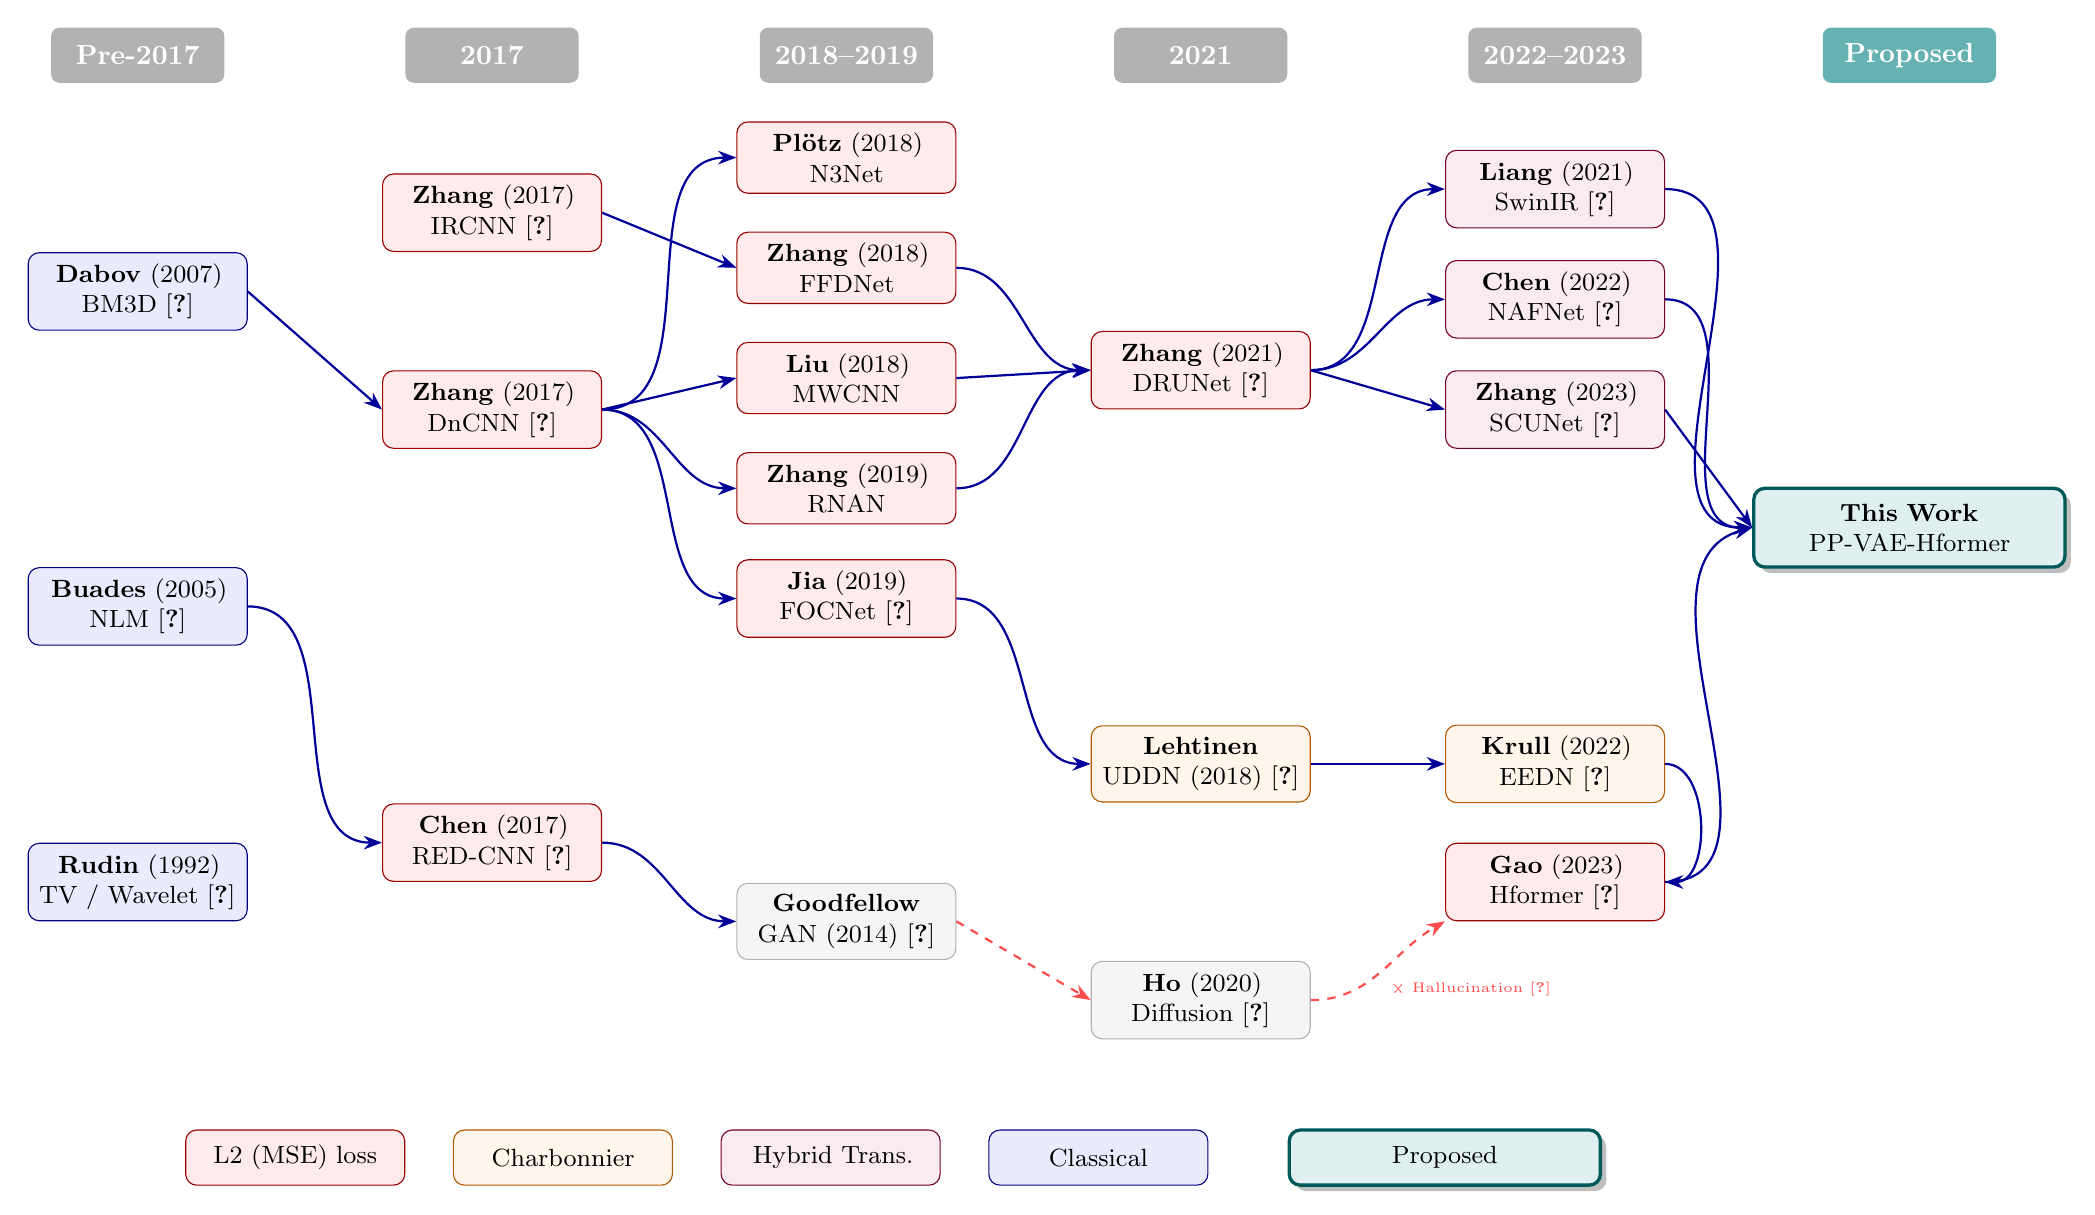
\begin{tikzpicture}[
    every node/.style={font=\small},
    era/.style={font=\normalsize\bfseries, text=white, fill=gray!60, rounded corners=3pt,
                minimum width=2.2cm, minimum height=0.7cm, align=center},
    classical/.style={draw=blue!50!black, fill=blue!8, rounded corners=4pt,
                      text width=2.5cm, align=center, inner sep=4pt, minimum height=0.9cm},
    cnnl2/.style={draw=red!60!black, fill=red!8, rounded corners=4pt,
                  text width=2.5cm, align=center, inner sep=4pt, minimum height=0.9cm},
    charb/.style={draw=orange!70!black, fill=orange!8, rounded corners=4pt,
                  text width=2.5cm, align=center, inner sep=4pt, minimum height=0.9cm},
    transformer/.style={draw=purple!60!black, fill=purple!8, rounded corners=4pt,
                        text width=2.5cm, align=center, inner sep=4pt, minimum height=0.9cm},
    generative/.style={draw=gray!60, fill=gray!8, rounded corners=4pt,
                       text width=2.5cm, align=center, inner sep=4pt, minimum height=0.9cm},
    proposed/.style={draw=teal!70!black, fill=teal!12, rounded corners=4pt,
                     text width=3.6cm, align=center, inner sep=5pt, minimum height=1.0cm,
                     very thick, drop shadow},
    >=Stealth,
    arr/.style={->, thick, blue!60!black},
    harr/.style={->, thick, red!70, dashed},
  ]

  %% ================= ERA LABELS =================
  \node[era] at (0,    7.5) {Pre-2017};
  \node[era] at (4.5,  7.5) {2017};
  \node[era] at (9.0,  7.5) {2018--2019};
  \node[era] at (13.5, 7.5) {2021};
  \node[era] at (18.0, 7.5) {2022--2023};
  \node[era, fill=teal!60] at (22.5, 7.5) {Proposed};

  %% ================= NODES =================

  %% Pre-2017 (X = 0)
  \node[classical] (bm3d) at (0, 4.5) {\textbf{Dabov} (2007)\\BM3D \cite{dabov_image_2007}};
  \node[classical] (nlm)  at (0, 0.5) {\textbf{Buades} (2005)\\NLM \cite{buades_non-local_2005}};
  \node[classical] (tv)   at (0, -3.0) {\textbf{Rudin} (1992)\\TV / Wavelet \cite{rudin_nonlinear_1992}};

  %% 2017 (X = 4.5)
  \node[cnnl2] (ircnn)  at (4.5, 5.5)  {\textbf{Zhang} (2017)\\IRCNN \cite{zhang_beyond_2017}};
  \node[cnnl2] (dncnn)  at (4.5, 3.0)  {\textbf{Zhang} (2017)\\DnCNN \cite{zhang_beyond_2017}};
  \node[cnnl2] (redcnn) at (4.5, -2.5) {\textbf{Chen} (2017)\\RED-CNN \cite{chen_low-dose_2017}};

  %% 2018--2019 (X = 9.0)
  \node[cnnl2] (n3net)  at (9.0, 6.2)  {\textbf{Plötz} (2018)\\N3Net};
  \node[cnnl2] (ffdnet) at (9.0, 4.8)  {\textbf{Zhang} (2018)\\FFDNet};
  \node[cnnl2] (mwcnn)  at (9.0, 3.4)  {\textbf{Liu} (2018)\\MWCNN};
  \node[cnnl2] (rnan)   at (9.0, 2.0)  {\textbf{Zhang} (2019)\\RNAN};
  \node[cnnl2] (focnet) at (9.0, 0.6)  {\textbf{Jia} (2019)\\FOCNet \cite{jia2019focnet}};
  \node[generative] (gan) at (9.0, -3.5) {\textbf{Goodfellow}\\GAN (2014) \cite{goodfellow_generative_2014}};

  %% 2021 (X = 13.5)
  \node[cnnl2] (drunet) at (13.5, 3.5) {\textbf{Zhang} (2021)\\DRUNet \cite{zhang_drunet_2021}};
  \node[charb] (uddn)   at (13.5, -1.5) {\textbf{Lehtinen}\\UDDN (2018) \cite{luo_uddn_2021}};
  \node[generative] (diffusion) at (13.5, -4.5) {\textbf{Ho} (2020)\\Diffusion \cite{ho_denoising_2020}};

  %% 2022--2023 (X = 18.0)
  \node[transformer] (swinir)  at (18.0, 5.8) {\textbf{Liang} (2021)\\SwinIR \cite{liang_swinir_2021}};
  \node[transformer] (nafnet)  at (18.0, 4.4) {\textbf{Chen} (2022)\\NAFNet \cite{chen_nafnet_2022}};
  \node[transformer] (scunet)  at (18.0, 3.0) {\textbf{Zhang} (2023)\\SCUNet \cite{zhang_scunet_2023}};
  \node[charb] (eedn)          at (18.0, -1.5) {\textbf{Krull} (2022)\\EEDN \cite{luo_eedn_2022}};
  \node[cnnl2] (hformer)       at (18.0, -3.0) {\textbf{Gao} (2023)\\Hformer \cite{zhang_hformer_2023}};

  %% Proposed (X = 22.5)
  \node[proposed] (proposed) at (22.5, 1.5) {\textbf{This Work}\\PP-VAE-Hformer};

  %% ================= EVOLUTION ARROWS =================

  %% Pre-2017 → 2017
  \draw[arr] (bm3d.east) -- (dncnn.west);
  \draw[arr] (nlm.east)  to[out=0, in=180] (redcnn.west);

  %% 2017 → 2018--2019
  \draw[arr] (ircnn.east)  -- (ffdnet.west);
  \draw[arr] (dncnn.east)  to[out=0, in=180] (n3net.west);
  \draw[arr] (dncnn.east)  -- (mwcnn.west);
  \draw[arr] (dncnn.east)  to[out=0, in=180] (rnan.west);
  \draw[arr] (dncnn.east)  to[out=0, in=180] (focnet.west);
  \draw[arr] (redcnn.east) to[out=0, in=180] (gan.west);

  %% 2018--2019 → 2021
  \draw[arr] (ffdnet.east) to[out=0, in=180] (drunet.west);
  \draw[arr] (mwcnn.east)  -- (drunet.west);
  \draw[arr] (rnan.east)   to[out=0, in=180] (drunet.west);
  \draw[arr] (focnet.east) to[out=0, in=180] (uddn.west);

  %% 2021 → 2022--2023
  \draw[arr] (drunet.east) to[out=0, in=180] (swinir.west);
  \draw[arr] (drunet.east) to[out=0, in=180] (nafnet.west);
  \draw[arr] (drunet.east) -- (scunet.west);
  \draw[arr] (uddn.east)   -- (eedn.west);

  %% EEDN → Hformer (routes AROUND the right side, NOT crossing the box)
  \draw[arr] (eedn.east) to[out=0, in=0] (hformer.east);

  %% Convergence → Proposed
  \draw[arr] (swinir.east)  to[out=0, in=180] (proposed.west);
  \draw[arr] (nafnet.east)  to[out=0, in=180] (proposed.west);
  \draw[arr] (scunet.east)  -- (proposed.west);
  \draw[arr] (hformer.east) to[out=0, in=195] (proposed.west);

  %% Generative warning (dashed, below main flow)
  \draw[harr] (gan.east)       -- (diffusion.west);
  \draw[harr] (diffusion.east) to[out=0, in=210]
    node[midway, below right, font=\tiny, text=red!70] {\texttimes\ Hallucination \cite{bhadra_hallucinations_2021}} (hformer.south west);

  %% ================= LEGEND =================
  \begin{scope}[shift={(2.0, -6.5)}]
    \node[cnnl2, minimum width=2.3cm, minimum height=0.7cm]       at (0, 0)   {L2 (MSE) loss};
    \node[charb, minimum width=2.3cm, minimum height=0.7cm]       at (3.4, 0) {Charbonnier};
    \node[transformer, minimum width=2.3cm, minimum height=0.7cm] at (6.8, 0) {Hybrid Trans.};
    \node[classical, minimum width=2.3cm, minimum height=0.7cm]   at (10.2, 0){Classical};
    \node[proposed, minimum width=2.3cm, minimum height=0.7cm]    at (14.6, 0){Proposed};
  \end{scope}

  \end{tikzpicture}
  } % End of resizebox
   \caption{Evolution of image denoising architectures from classical methods (2007) through to the proposed PP-VAE-Hformer.}
   \label{fig:architecture_evolution}
   \caption*{\footnotesize \textit{Note:} Arrows indicate conceptual inheritance or direct extension. Colour indicates loss function family: red = MSE/L2; orange = Charbonnier; purple = hybrid Transformer; teal = proposed composite. Citations refer to the corresponding publications in the bibliography.}
\end{figure}
\end{landscape}
% ============================================================
\section{Critical Analysis of Literature, Research Motivation, and Gap Identification}
\label{sec:intro:gap}
% ============================================================

The overarching challenge revealed by the existing literature is an irreconcilable tension
between perceptual realism and structural, pathological fidelity. A systematic review of
current medical image reconstruction frameworks exposes a perilous clinical reality:
algorithms optimised purely for visual appeal, such as GANs and unconstrained diffusion
models, jeopardise patient safety by hallucinating non-existent anatomy
\cite{bhadra_hallucinations_2021}, whilst algorithms optimised for absolute pixel-wise error
(CNNs and standard VAEs) compromise diagnosis by over-smoothing and obliterating subtle
disease \cite{zhao_loss_2017, bredell_explicitly_2023}.

The concept of hallucination in tomographic and radiographic reconstruction is currently the
subject of intense critical scrutiny within the medical physics and health data science
communities. As Bhadra et al.\ \cite{bhadra_hallucinations_2021} meticulously demonstrated
using formal mathematical analysis, an inaccurate learned prior in deep generative networks
forces the algorithmic manifestation of false structural properties, yielding a quantifiable
``hallucination map.'' In a clinical setting, an algorithm hallucinating a pulmonary nodule
where none exists, or, conversely, hallucinating healthy lung tissue over a developing
pneumothorax, carries disastrous medico-legal and diagnostic implications. Similarly, Kc
et al.\ \cite{kc_sfrc_2024} highlighted that while deep learning outputs may appear visually
appealing to human observers, the absence of robust, pathology-preserving mathematical
constraints inevitably leads to the synthesis of spurious edge details undetectable by
standard pixel-fidelity metrics.

Conversely, the probabilistic and interpretable nature of the VAE provides an optimal
theoretical foundation for safe medical deployment, primarily because it avoids the
adversarial instability of GANs and offers natural uncertainty quantification
\cite{kingma_introduction_2019}. However, as previously established, its clinical translation
has been blocked by the blur error \cite{bredell_explicitly_2023}.

Recent breakthrough literature presented at the International Conference on Learning
Representations (ICLR) 2023 by Bredell, Flouris et al.\ \cite{bredell_explicitly_2023}
fundamentally redefined the mathematical boundaries of VAE reconstruction. Bredell et al.\
identified that standard VAEs fail to capture high frequencies because the assumed identity
covariance matrix in the Gaussian likelihood fails to map spatial frequency correlations. They
proposed explicitly minimising the blur error by assuming an image-specific blurring kernel in
the frequency domain, mathematically framing the reconstruction via Wiener deconvolution.
By utilising a block-circulant covariance matrix, their formulation allows the VAE to retain its
mathematical connection to ELBO likelihood maximisation while forcing the network to
explicitly penalise blurry generations in the Fourier domain.

Despite these profound theoretical advancements, a distinct and critical research gap remains.

\textbf{Gap 1: Lack of Paediatric Specificity and Pathology Focus.} Existing evaluations of
advanced VAEs, including the blur-minimising formulations by Bredell et al., focus largely
on high-resolution natural image datasets (e.g., CelebA \cite{liu_deep_2015}) or clean,
high-contrast adult MRI slices. These studies bypass the uniquely challenging domain of the
paediatric chest X-ray, which is characterised by distinct anatomical proportions, high
dynamic range, and severe Poisson-Gaussian noise corruption \cite{yang_medmnist_2023}.
Furthermore, while minimising global blur is a significant step forward, preserving specific
diagnostic pathology, such as the faint, hazy opacities of a viral pneumonia, requires more
than frequency-domain sharpening alone. It requires a dedicated, multi-constraint objective
function that simultaneously addresses spatial accuracy, edge retention, and perceptual
intelligence.

\textbf{Gap 2: Absence of Multi-Constraint Regularisation in Probabilistic Frameworks.}
Current literature lacks VAE reconstruction frameworks explicitly designed and constrained to
preserve pathology. The field relies heavily on single-metric loss functions. A framework
combining structural similarity objectives, perceptual feature matching, pixel-wise fidelity,
and spatial edge preservation within a stochastic ELBO envelope remains largely unexplored
for paediatric thoracic imaging.

\textbf{Gap 3: Uncertainty Quantification as a Clinical Requisite.} While VAEs naturally
support uncertainty quantification, very few studies leverage this capability to provide
clinically actionable pixel-level confidence maps alongside the reconstructed radiograph
\cite{kendall_what_2017}. In deterministic models, clinicians are forced to blindly trust the enhanced image. Providing a spatial map of epistemic uncertainty is a necessary step to bridge the gap between algorithm design and clinical trust.

\textbf{Gap 4: Absence of Explicit Frequency-Domain Regularisation.} Although the spectral bias of neural networks is a rigorously proven, universal property of gradient-based training \cite{rahaman_spectral_2019, xu_frequency_2020}, no existing denoising framework for paediatric radiograph enhancement includes an explicit loss penalty that directly targets discrepancies in the frequency spectrum of the reconstructed image. The practical consequence is that all existing reconstruction algorithms, regardless of their spatial-domain constraints, implicitly permit systematic errors in the high-frequency content of the output. As demonstrated by Durall et al.\ \cite{durall_watch_2020}, even visually convincing deep neural network outputs can contain measurable, clinically significant distortions in their spectral power distribution when examined in the frequency domain. These distortions occur specifically in the high-frequency range that carries the fine diagnostic detail of paediatric pathology. A loss function that operates directly in the Fourier domain, computing how different the frequency composition of the reconstruction is from the target, provides a direct mechanism to correct this systematic spectral error. Without such a constraint, the high-frequency clinical content that spectral bias neglects will remain under-recovered, regardless of how well the spatial-domain losses perform.
Table~\ref{tab:intro:gaps} synthesises these identified gaps, their evidence base, clinical
consequences, and the proposed framework's solutions. The primary literature underpinning
each gap is reviewed in depth in Chapter~\ref{chap:lit}.

\begin{table}[htbp]
  \centering
  \caption{Gap synthesis in medical image enhancement. Each identified limitation maps to a
  specific design decision in the proposed PP-VAE framework.}
  \label{tab:intro:gaps}
  \small
  \begin{tabularx}{\textwidth}{
    >{\raggedright\arraybackslash}p{2.8cm} 
    >{\raggedright\arraybackslash}p{2.2cm} 
    >{\raggedright\arraybackslash}X 
    >{\raggedright\arraybackslash}X
  }
    \toprule
    \textbf{Identified Limitation} &
    \textbf{Evidence Base} &
    \textbf{Clinical Consequence} &
    \textbf{Proposed Solution (PP-VAE)} \\
    \midrule
    Hallucination of anatomical structures
    & \cite{bhadra_hallucinations_2021, kc_sfrc_2024}
    & False-positive diagnoses; erroneous surgical or therapeutic interventions.
    & Avoid pure adversarial objectives; rely on constrained, regularised probabilistic decoders (VAE). \\
    \midrule
    Loss of subtle pathology (over-smoothing)
    & \cite{bredell_explicitly_2023, zhao_loss_2017}
    & False-negative interpretations; failure to detect early-stage pneumonia or interstitial disease.
    & Integrate edge-preservation ($\mathcal{L}_\mathrm{Edge}$) and structural similarity ($\mathcal{L}_\mathrm{SSIM}$) constraints directly into the VAE loss. \\
    \midrule
    Blur-induced error in VAE latent modelling
    & \cite{bredell_explicitly_2023}
    & Concealment of sharp anatomical margins; degraded diagnostic feature extraction.
    & Reformulate VAE reconstruction loss incorporating spatial and frequency-domain penalties without violating the ELBO. \\
    \midrule
    Lack of paediatric CXR specificity
    & \cite{kermany_identifying_2018, laborie_scoping_2026, strauss_image_2009}
    & Models generalise poorly to the unique anatomy, pathology, and low-dose constraints of children.
    & Train and validate exclusively on the full Kermany 2018 paediatric CXR dataset at 256\,$\times$\,256 pixels \cite{kermany_identifying_2018}. \\
    \midrule
    Absence of uncertainty quantification
    & \cite{kendall_what_2017, ovadia_can_2019}
    & Clinicians cannot ascertain algorithmic confidence, leading to over-reliance or blind distrust.
    & Exploit the VAE stochastic latent space $q_\phi(z|x)$ to generate pixel-level epistemic uncertainty maps. \\
    \midrule
    \textbf{Absence of explicit frequency-domain regularisation}
    & \textbf{\cite{rahaman_spectral_2019, xu_frequency_2020, durall_watch_2020}}
    & \textbf{Systematic under-recovery of high-frequency pathological detail due to spectral bias; visually plausible but spectrally distorted reconstructions.}
    & \textbf{Add a Focal Frequency Loss term ($\mathcal{L}_\mathrm{Freq}$) that directly penalises discrepancies in the image frequency spectrum \cite{jiang_focal_2021}.} \\
    \bottomrule
  \end{tabularx}
\end{table}

% ============================================================
\section{Research Aims and Objectives}
\label{sec:intro:aims}
% ============================================================

The overarching aim of this dissertation is to directly address the highlighted clinical,
physical, and engineering gaps by designing, implementing, and rigorously validating a novel
Pathology-Preserving Variational Autoencoder (PP-VAE). This framework is specifically
engineered to enhance simulated low-dose paediatric chest radiographs, recovering
high-fidelity diagnostic images whilst mathematically suppressing the twin risks of structural
hallucination and over-smoothing. To achieve this primary aim, the research is structured
around the following specific scientific objectives:

\begin{enumerate}
  \item \textbf{Degradation Modelling:} To formulate and apply a mathematically rigorous
        Poisson-Gaussian degradation pipeline that accurately simulates realistic low-dose
        quantum and electronic noise profiles characteristic of paediatric chest radiography
        under ALARA protocols.

  \item \textbf{Architecture and Objective Design:} To construct a novel PP-VAE framework
        driven by a composite, multi-constraint loss function. This objective seeks to
        explicitly balance probabilistic latent regularisation (KL divergence) with pixel
        fidelity, high-frequency edge retention, perceptual structural similarity, and an
        explicit frequency-domain spectral fidelity penalty, directly counteracting
        the spectral bias of gradient-based neural network training
        \cite{rahaman_spectral_2019, xu_frequency_2020}.

  \item \textbf{Pathology Preservation Validation:} To train the proposed model on the
        full Kermany paediatric chest radiograph dataset \cite{kermany_identifying_2018}
        at 256\,$\times$\,256 pixel resolution and quantitatively assess its capacity to
        preserve critical diagnostic features, such as pneumonia consolidations, compared
        to five state-of-the-art denoising baselines (DnCNN, DRUNet, SwinIR, NAFNet,
        SCUNet) evaluated under the same Poisson-Gaussian noise conditions.

  \item \textbf{Uncertainty Quantification:} To exploit the probabilistic nature of the VAE's
        latent space to compute and evaluate pixel-wise uncertainty maps, providing a
        measurable, visual index of structural reliability to support safer clinical
        interpretation \cite{kendall_what_2017}.
\end{enumerate}

% ============================================================
\section{Contributions of This Work}
\label{sec:intro:contributions}
% ============================================================

The framework proposed in this dissertation, the PP-VAE-Hformer\footnote{PP-VAE-Hformer:
Pathology-Preserving Variational Autoencoder with an Hformer-inspired hybrid CNN-Transformer
backbone. The name reflects the three design priorities: (1) pathology preservation via the
composite loss, (2) probabilistic uncertainty via the VAE bottleneck, and (3) efficient
hybrid feature extraction via the Hformer architecture.}, differs from standard denoising
networks in two complementary ways. First, it replaces the standard single pixel-wise loss
with a composite, four-term objective that trains the network to optimise simultaneously for
pixel accuracy, structural similarity, spectral fidelity, and probabilistic well-posedness.
Second, it inserts a VAE probabilistic bottleneck\footnote{A VAE bottleneck compresses the
image into a probability distribution rather than a single fixed representation, then reconstructs
from a random sample drawn from that distribution. Running this sampling step multiple times
produces slightly different reconstructions, and the variance between them is the epistemic
uncertainty map.} into the Hformer encoder-decoder backbone, enabling both types of
uncertainty described in Section~\ref{sec:intro:existing:vae} to be estimated from a single
forward pass.

The composite loss comprises four terms (full specification in Chapter~\ref{chap:methods}): (i) the heteroscedastic NLL \cite{kendall_what_2017}, which predicts per-pixel aleatoric uncertainty $\hat{\sigma}_a$ alongside the reconstruction mean $\hat{\mu}$, replacing the unweighted MSE of all comparison architectures; (ii) multi-scale SSIM \cite{wang_multiscale_2003}, which penalises blurred structural regions that PSNR fails to detect; (iii) Focal Frequency Loss \cite{jiang_focal_2021}, the novel spectral-domain regulariser that adaptively concentrates the correction signal on the high-frequency components the network is currently reconstructing most poorly --- directly counteracting the spectral bias that suppresses fine pathological detail; and (iv) KL divergence \cite{kingma_auto-encoding_2014}, annealed cyclically to prevent posterior collapse and enable Monte Carlo epistemic uncertainty estimation. The combined objective is:

\begin{equation}
\label{eq:intro:totalloss}
\mathcal{L}_\mathrm{total} =
\mathcal{L}_\mathrm{NLL}
+ \beta\,\mathcal{L}_\mathrm{KL}
+ \lambda_{\mathrm{SSIM}}\,\mathcal{L}_\mathrm{SSIM}
+ \lambda_{\mathrm{FFL}}\,\mathcal{L}_\mathrm{FFL}
\end{equation}

This composite objective is evaluated through a five-arm ablation study: Arm~A uses only
an L2 loss and no VAE bottleneck (matching the training objective of every comparison
architecture); Arms~B through~D add terms one at a time (NLL, then NLL+SSIM, then
NLL+SSIM+FFL); Arm~E is the full PP-VAE-Hformer including the VAE bottleneck and KL
term. The ablation isolates the specific improvement attributable to each design decision.

The framework is trained and evaluated on the full Kermany et al.\ \cite{kermany_identifying_2018}
paediatric chest radiograph collection (5,856 images, patients aged 1--5 years, at
256\,$\times$\,256 pixel resolution), making it the first systematic comparison of
state-of-the-art denoising approaches on paediatric chest X-rays at clinically relevant
resolution. This is a direct response to the finding by Laborie et al.\
\cite{laborie_scoping_2026} that 18 of 20 AI models degrade in performance when applied
to paediatric populations.

The framework produces three outputs for each input image: a reconstructed mean
$\hat{\mu}$, an aleatoric uncertainty map $\hat{\sigma}^2_\mathrm{a}$ from the NLL head
(showing where the input was too noisy to recover reliably), and an epistemic uncertainty
map $\hat{\sigma}^2_\mathrm{e}$ from $K = 20$ Monte Carlo samples through the VAE
bottleneck (showing where the model is relying on its learned prior rather than the input
data). No comparison architecture produces any uncertainty output at all.

% ============================================================
\section{Dissertation Roadmap}
\label{sec:intro:roadmap}
% ============================================================

To address the research objectives and detail the development of the PP-VAE-Hformer,
this dissertation is structured as follows:

\begin{itemize}
  \item \textbf{Chapter 2 (Literature Review):} Synthesises the epidemiological evidence
        on paediatric radiation risk, reviews the Kermany dataset, traces the evolution of
        denoising architectures from BM3D through SCUNet, examines loss function design,
        reviews the documented failure of AI in paediatric radiology, and evaluates image
        quality metrics, concluding with the precise research gap the proposed framework
        addresses \cite{mathews_cancer_2013, hauptmann_brain_2023,
        bosch_de_basea_gomez_risk_2023, smith-bindman_hematologic_2025,
        laborie_scoping_2026, zhang_comprehensive_2012}.

  \item \textbf{Chapter 3 (Methods):} Details the Poisson-Gaussian noise model and its
        three severity presets, the Hformer backbone with VAE bottleneck and dual
        uncertainty heads, the four-term composite loss, the five-arm ablation design,
        the training protocol including KL annealing, and the evaluation metrics
        (PSNR, SSIM, FSIM, LPIPS, ECE) \cite{kendall_what_2017, jiang_focal_2021,
        zhang_fsim_2011}.

  \item \textbf{Chapter 4 (Results):} Presents ablation results across all 16 arms at
        three noise levels, comparison against retrained KAIR baselines (FFDNet, IRCNN, DRUNet, SwinIR) and DnCNN,
        uncertainty map visualisations showing aleatoric and epistemic outputs, and
        calibration analysis via Expected Calibration Error.

  \item \textbf{Chapter 5 (Discussion):} Interprets the findings in the context of the
        radiation risk evidence, examines where the composite loss provides measurable
        gain over MSE, discusses the clinical meaning of the uncertainty maps, and
        identifies the limitations of the proposed framework.

  \item \textbf{Chapter 6 (Conclusion):} Summarises the scientific contributions, directly
        answers the research aims, and outlines concrete avenues for future clinical
        translation.
\end{itemize}


% ============================================================
% CHAPTER 2 — LITERATURE REVIEW
% ============================================================
\chapter{Literature Review}
\label{chap:lit}

This chapter reviews the evidence and technical background that motivates and situates the
proposed framework. The review proceeds in five stages. First, it sets out the clinical case for
paediatric chest radiograph denoising by synthesising the epidemiological evidence on
radiation risk in children, a body of literature that has grown substantially in the last
decade and now provides direct, quantified justification for algorithmic dose reduction. Second,
it describes the Kermany paediatric chest X-ray dataset that provides the experimental
substrate for this work. Third, it traces the evolution of image denoising methods from
classical signal processing to current state-of-the-art deep learning architectures, evaluating
each approach against the specific demands of the clinical problem. Fourth, it examines the
design of loss functions for image restoration, which is the domain of the principal
contribution made by this dissertation. Fifth, it reviews uncertainty quantification in medical
imaging and the documented failure of general-purpose artificial intelligence when applied to
paediatric radiology. The chapter concludes by synthesising these strands into the precise
research gap that the proposed framework addresses.

% ============================================================
\section{The Clinical Case for Paediatric CXR Denoising: Radiation Risk as Direct Justification}
\label{sec:lit:radiation}
% ============================================================

The motivation for this dissertation is not abstract. Children who receive medical imaging
examinations using ionising radiation carry a quantifiable, dose-dependent risk of developing
cancer later in life. This section sets out that evidence base in full, because it is the
direct and primary justification for investing in algorithms that reduce the radiation dose
required to achieve a clinically useful radiograph.

% ─────────────────────────────────────────────────────────
\subsection{The Epidemiological Evidence Base}
\label{sec:lit:radiation:evidence}
% ─────────────────────────────────────────────────────────

Until relatively recently, the harmful effects of low-dose diagnostic radiation in children
rested largely on extrapolation from atomic bomb survivor data and the Linear No-Threshold
(LNT) model endorsed by the ICRP and the BEIR VII committee
\cite{international_commission_on_radiological_protection_2007_2007,
national_research_council_health_2006}.\footnote{The Linear No-Threshold model holds
that any amount of ionising radiation carries some risk of cancer induction, however small,
with no lower threshold of safe exposure.} In the past decade, four independent large-scale
cohort studies have replaced inference with direct observation.

Mathews et al.\ \cite{mathews_cancer_2013} conducted a retrospective cohort study of
approximately 680,000 children in Australia who received computed tomography\footnote{Computed
tomography (CT), sometimes called a CAT scan, produces cross-sectional images of the body
using a rotating X-ray beam. It delivers substantially higher radiation doses than a plain
chest X-ray.} before the age of 19 years, following them for up to 24 years. Children
exposed to CT showed an overall incidence rate ratio of 1.24 for all cancers combined, with
the risk rising by 0.16 for each additional CT examination. This was one of the first studies
to demonstrate directly observed excess cancer incidence following CT exposure in a
paediatric population, rather than relying on modelled projections.

The European EPI-CT consortium subsequently followed 948,174 paediatric and young adult
patients across nine countries with improved individual dosimetry. Hauptmann et al.\
\cite{hauptmann_brain_2023}, reporting on brain and central nervous system tumours, found
an excess relative risk (ERR)\footnote{Excess relative risk per 100 mGy is a measure of how
much extra cancer risk is added for every 100 milligray of absorbed radiation dose. An ERR
of 1.27 means the relative risk of developing the cancer increases by 127\,\% for every
100 mGy.} of 1.27 per 100\,mGy. Translating this to an accessible absolute number: for every
10,000 children who receive one head CT examination, approximately one additional brain
cancer is expected within 5 to 15 years of exposure. Bosch de Basea Gomez et al.\
\cite{bosch_de_basea_gomez_risk_2023}, analysing the same EPI-CT cohort for haematological
malignancies,\footnote{Haematological malignancies are blood cancers, including leukaemia and
lymphoma.} reported an ERR of 1.96 per 100\,mGy. Critically, their analysis detected
statistically elevated risk at active bone marrow doses as low as 10--15\,mGy, a level
achievable from a single paediatric chest CT after contemporary dose optimisation. Between
one and two haematological cancers are expected per 10,000 children at the mean CT dose
used in the cohort.

The most comprehensive recent evidence comes from Smith-Bindman et al.\
\cite{smith-bindman_hematologic_2025}, who followed 3.7 million children across the United
States and Canada in the Radiation-Induced Cancer (RIC) study, published in the
\textit{New England Journal of Medicine}. This study is particularly important because it is
the first to quantify radiation doses and cancer risks across all imaging modalities within a
single cohort. Their main findings are summarised in Table~\ref{tab:lit:dose}.

\begin{table}[H]
  \centering
  \caption{Radiation dose and attributable cancer risk by imaging modality in children.}
  \label{tab:lit:dose}
  \small
  \begin{tabular}{l c c c}
    \toprule
    \textbf{Modality} &
    \textbf{Mean bone marrow dose (mGy)} &
    \textbf{ERR per 100 mGy} &
    \textbf{Attributable cancer risk} \\
    \midrule
    Chest radiograph & 0.01 & --- & 0.03\,\% \\
    Chest CT          & 2.8  & 2.54 & 6.0\,\% \\
    Head CT           & 13.7 & 2.54 & 25.9\,\% \\
    Abdominal CT      & 10.4 & 2.54 & 21.4\,\% \\
    \bottomrule
  \end{tabular}

  \vspace{0.01em}
  {\footnotesize \textbf{Note:} The contrast between chest radiography and head CT (a factor
  of over 800 in attributable risk) illustrates why preventing unnecessary escalation from
  X-ray to CT is clinically meaningful. ERR = excess relative risk. Source: Smith-Bindman 
  et al.\ (2025), \textit{N Engl J Med}, 392(1):44--56.}
\end{table}

The key finding for this dissertation is the roughly 1,400-fold difference in bone marrow
dose between a chest radiograph (0.01\,mGy) and a CT of the head (13.7\,mGy). A single
chest radiograph carries approximately 0.03\,\% attributable cancer risk; a single head CT
carries 25.9\,\%. The risk estimates across all four studies are consistent, converging on
an ERR of approximately 1.3 to 2.5 per 100\,mGy depending on cancer type
\cite{mathews_cancer_2013, hauptmann_brain_2023, bosch_de_basea_gomez_risk_2023,
smith-bindman_hematologic_2025}. That consistency across different populations, different
dosimetry methods, and different follow-up periods is not coincidence. It reflects the weight
of direct observational evidence that diagnostic radiation causes cancer in children at doses
encountered in routine clinical care.

% ─────────────────────────────────────────────────────────
\subsection{Why Preventing Imaging Escalation Is the Key Mechanism}
\label{sec:lit:radiation:escalation}
% ─────────────────────────────────────────────────────────

A chest radiograph at 0.01\,mGy carries near-zero cancer risk per examination. This does
not mean clinicians can be complacent about chest X-ray quality. It means exactly the
opposite: the chest X-ray is the one modality that does not generate meaningful radiation
risk per exam, so it should be used as effectively as possible to avoid escalation to modalities
that do.

When a chest radiograph is of insufficient diagnostic quality, clinical teams face three
options. They can repeat the radiograph at a higher dose or with corrected positioning.
They can accept diagnostic uncertainty and manage the patient conservatively, risking a
missed diagnosis. Or they can escalate to CT, which delivers a bone marrow dose
approximately 280 times higher than the original radiograph for a chest study, and more than
1,000 times higher if a head CT is required \cite{smith-bindman_hematologic_2025}. Effective
denoising removes this dilemma. A low-dose chest X-ray that is computationally enhanced to
diagnostic standard does not need to be repeated, and does not push clinical teams toward CT.
The per-exam radiation burden remains at 0.01\,mGy.

Children with chronic conditions are particularly exposed to this risk. Neonates in intensive
care units, children with cystic fibrosis, congenital heart disease, or bronchopulmonary
dysplasia often accumulate tens to hundreds of chest radiographs over their early years
\cite{johnson_cumulative_2014}. Even at 0.01\,mGy per exam, cumulative dose accumulates
across a childhood of repeated imaging. More importantly, each inadequate image creates
pressure for a repeat acquisition or CT upgrade. A reliable denoising algorithm that
consistently achieves diagnostic quality at minimum exposure reduces the per-exam dose
target, the repeat rate, and the CT escalation rate, all of which compound over a child's
imaging history \cite{smith-bindman_hematologic_2025, mathews_cancer_2013}.

This three-tier hierarchy -- chest radiograph first, then lung ultrasound, then CT only for
complex or refractory cases -- has been formally codified in European clinical practice.
Lovrenski et al.\ \cite{lovrenski_esr_2025}, writing on behalf of the European Society of
Paediatric Radiology (ESPR) with endorsement from the European Society of Radiology
executive bodies, published practice recommendations in 2025 stating that ``chest radiograph
and lung ultrasound should be used as the initial diagnostic tools for paediatric pulmonary
diseases,'' with CT ``reserved for complex cases.'' Lung ultrasound (LUS)\footnote{Lung
ultrasound uses high-frequency sound waves rather than ionising radiation to image the lungs
and pleural space. It is radiation-free, immediately available at the bedside, and
particularly sensitive for pleural effusions, consolidations, and subpleural abnormalities.}
is radiation-free, immediate, and specifically sensitive for pleural, subpleural, and
consolidation findings -- precisely the findings that are diagnostically decisive in paediatric
pneumonia and its complications. The ESPR recommendation therefore establishes that this
dissertation's engineering objective -- making low-dose chest radiographs as diagnostically
complete as possible -- is not an academic hypothesis but the direct operationalisation of
European clinical best practice. The algorithm proposed here does not replace the ESPR
pathway; it protects the maximum number of clinical decisions within the lowest-radiation
tier of that pathway.

% ============================================================
\section{The Kermany Paediatric Chest X-Ray Dataset}
\label{sec:lit:kermany}
% ============================================================

The primary dataset for this dissertation is the paediatric chest X-ray collection assembled
by Kermany et al.\ \cite{kermany_identifying_2018} at the Guangzhou Women and Children's
Medical Centre in China, published in \textit{Cell} in 2018. The collection comprises 5,856
anterior-to-posterior\footnote{Anterior-to-posterior technique refers to radiation beam passing thru the front chest and the sensor plate being behind the shoulder blades as opposed to posterior-anterior,  the standard technique used in adults.} chest radiographs from children aged one to five years, acquired and
labelled for binary clinical classification: pneumonia (bacterial or viral) versus normal. The
dataset is publicly available and has been extensively used in applied machine learning
research for respiratory disease classification \cite{kermany_identifying_2018}.

The dataset is structured into a training set of 5,232 images and a test set of 624 images,
with the training set further divided into Normal (1,349 images) and Pneumonia (3,883
images) subfolders. This class imbalance, with approximately 74\,\% of training images
showing pneumonia, reflects the clinical reality of the source population: children referred
for chest radiography at a paediatric hospital with known respiratory symptoms are more
likely to have pneumonia than not.

For the denoising task in this dissertation, class labels are not used during training.
Instead, all images serve as clean reference targets, to which simulated Poisson-Gaussian
noise is applied on-the-fly during batch loading to generate paired (noisy, clean) training
examples. This supervised setup, described in detail in Chapter~3, means that every
training example has a known ground truth against which the model's reconstruction is
evaluated. Images are stored as JPEG files with variable native resolution ranging from
approximately 400 to 1,400 pixels in each dimension; all images are resized to
256\,$\times$\,256 pixels for training to standardise computational requirements while
retaining the full-resolution diagnostic content that distinguishes this dataset from
the 28\,$\times$\,28 pixel MedMNIST \cite{yang_medmnist_2023} version derived from the same source.

The choice of the full-resolution Kermany collection\cite{kermany_identifying_2018}, rather than the smaller MedMNIST\cite{yang_medmnist_2023}
derivative, is motivated by two considerations. Paediatric chest radiograph denoising is a
high-frequency recovery problem: the fine interstitial markings, pleural edges, and
consolidation margins that carry diagnostic information about pneumonia exist at spatial
scales that are simply not present in a 28-pixel image. Demonstrating that the proposed
framework operates at clinically relevant resolutions is a prerequisite for any claim of
clinical utility. Additionally, the comparison architectures reviewed in
Section~\ref{sec:lit:architectures} were all designed and benchmarked on full-resolution
images; a fair comparison requires a shared/similar resolution regime.

% ============================================================
\section{The Evolution of Image Denoising Architectures}
\label{sec:lit:architectures}
% ============================================================

Image denoising has a long research history, and the field has undergone rapid change (Figure~\ref{fig:architecture_evolution}) in the
past decade as deep learning has displaced classical signal processing methods. This section
traces that trajectory and evaluates each class of method against the requirements of
paediatric CXR denoising.

% ─────────────────────────────────────────────────────────
\subsection{Classical Methods}
\label{sec:lit:architectures:classical}
% ─────────────────────────────────────────────────────────

Classical denoising approaches operate entirely without learned data representations.
Block-Matching and 3D Filtering (BM3D), introduced by Dabov et al.\ \cite{dabov_image_2007},
groups similar image patches from across the image, stacks them into a three-dimensional
array, applies a joint transform domain filter, and reconstructs each patch by averaging over
its matched group. BM3D was for many years the reference standard for Gaussian denoising,
achieving a peak signal-to-noise ratio\footnote{Peak Signal-to-Noise Ratio (PSNR), measured in
decibels, compares the maximum possible pixel intensity to the level of background noise.
Higher PSNR indicates better image quality, but it does not always correlate with how
diagnostic the image looks to a clinician.} of 28.57\,dB on the standard BSD68
benchmark at noise level $\sigma = 25$ \cite{dabov_image_2007}. Non-Local Means (NLM)
\cite{buades_non-local_2005} takes a related approach, estimating each pixel as a
weighted average of all pixels in the image whose neighbourhood resembles the target
neighbourhood.

Classical methods have a fundamental limitation in the medical imaging context: they cannot
distinguish between noise and fine anatomical detail, because they operate entirely on
statistical self-similarity without any semantic understanding of what the image contains.
Total variation regularisation, for example, forces the denoised image to be piecewise
smooth, systematically erasing the fine interstitial reticulations and vessel wall margins
that are relevant for diagnosing subtle respiratory infections \cite{rudin_nonlinear_1992}.
BM3D achieves strong average PSNR but at the cost of over-smoothing textures that would
be classified as noise by a purely statistical criterion and as clinically meaningful by a
radiologist.

% ─────────────────────────────────────────────────────────
\subsection{Convolutional Neural Networks}
\label{sec:lit:architectures:cnn}
% ─────────────────────────────────────────────────────────

The first generation of deep learning denoisers was based on convolutional neural
networks.\footnote{A convolutional neural network (CNN) processes images by repeatedly
applying small, learnable filters to local patches of the image. Each filter detects a
different visual pattern, and successive layers detect increasingly complex structures, from
simple edges to entire anatomical shapes.} Zhang et al.\ \cite{zhang_beyond_2017}
introduced the Denoising Convolutional Network (DnCNN) for blind Gaussian denoising, a
17-layer residual network\footnote{A residual network adds the input of each layer directly
to its output, allowing the network to learn only the difference (the residual) between input
and output, rather than the full transformation. This stabilises training and allows much
deeper networks.} that learns to predict the noise component rather than the clean image
directly. DnCNN achieved 29.23\,dB on BSD68 at $\sigma = 25$, a gain of 0.66\,dB over
BM3D, and established residual learning as the standard paradigm for supervised
denoising \cite{zhang_beyond_2017}.

For medical imaging, Chen et al.\ \cite{chen_low-dose_2017} adapted the encoder-decoder U-Net
architecture of Ronneberger et al.\ \cite{ronneberger_u-net_2015} to produce RED-CNN
(Residual Encoder-Decoder CNN) for low-dose CT denoising, demonstrating that skip
connections between the encoder and decoder preserved fine anatomical structures that were
otherwise smoothed out by bottleneck compression. Luo et al.\ \cite{luo_uddn_2021}
subsequently introduced UDDN (Ultra-Dense Denoising Network) for cardiac catheter X-ray
denoising, incorporating dense connectivity\footnote{Dense connectivity means that each
layer receives feature maps from all previous layers, not just the immediately preceding one.
This encourages feature reuse and allows the network to maintain fine-grained information
across many processing steps.} based on the DenseNet architecture \cite{huang_densely_2017}.
A follow-up by the same group, the Edge-Enhancement DenseNet (EEDN) \cite{luo_eedn_2022},
added a dedicated frequency-decomposition branch to recover high-frequency edge detail
separately from low-frequency structural content following comments like "artificial looking lungs" from their former network's (UDDN) output images by blinded cardiologists.

The most capable pure CNN denoiser is DRUNet \cite{zhang_drunet_2021}, a deep U-Net
with 32.7 million parameters that accepts the noise level as an explicit input alongside the
degraded image, allowing a single trained model to handle a continuous range of noise
levels. DRUNet achieved 29.48\,dB on BSD68 at $\sigma = 25$, setting the practical ceiling
for CNN-based denoising \cite{zhang_drunet_2021}.

All CNN denoisers share a common limitation. They are trained to minimise a pixel-wise
loss, typically mean squared error (MSE) or mean absolute error (MAE). As Zhao et al.\
\cite{zhao_loss_2017} systematically demonstrated, networks trained under MSE converge
to the conditional mean of all plausible clean images consistent with the noisy input. This
averaging over multiple plausible reconstructions manifests as spatial blurring. A
consolidating pneumonia presents a wide range of possible intensity values across different
patients; the network learns to output a blurred, average intensity that minimises the
squared error but destroys the sharp boundary between diseased and healthy lung tissue.

% ─────────────────────────────────────────────────────────
\subsection{Transformer and Hybrid Architectures}
\label{sec:lit:architectures:transformer}
% ─────────────────────────────────────────────────────────

The introduction of the Transformer architecture \cite{vaswani_attention_2017}, originally
developed for natural language processing, opened a new direction in image denoising.
Convolutional filters are constrained to local spatial neighbourhoods: a filter with a
3\,$\times$\,3 pixel kernel cannot directly compare pixels that are 50 pixels apart.
The self-attention mechanism\footnote{Self-attention allows every position in an image to
directly compare itself with every other position, regardless of distance. This captures
long-range dependencies such as the symmetric layout of the lungs, or the consistent
texture of a pneumonic consolidation across a large anatomical region.} in Transformers
removes this constraint, enabling each image position to gather information from any other
position regardless of distance.

Liang et al.\ \cite{liang_swinir_2021} applied the Shifted Window Transformer (Swin
Transformer \cite{liu_swin_2021}) to image restoration, producing SwinIR. Rather than
computing self-attention across the full image, which would require memory quadratic in
the number of pixels, SwinIR partitions the image into non-overlapping windows of
8\,$\times$\,8 pixels and alternates between fixed and shifted window configurations to
allow information to cross window boundaries \cite{liang_swinir_2021}. SwinIR achieved
29.50\,dB on BSD68 at $\sigma = 25$, a marginal improvement over DRUNet, confirming
that Transformer-based long-range context provides a small but consistent benefit over
CNN-only architectures for natural image denoising \cite{liang_swinir_2021}.

Zhang et al.\ \cite{zhang_hformer_2023} introduced Hformer (Hybrid Transformer) for
low-dose CT denoising. With only 1.65 million parameters, Hformer achieves competitive
performance by alternating convolutional residual blocks with lightweight Transformer
attention blocks, with skip connections spanning all encoder-decoder scales. The small
parameter count is particularly important in the medical imaging context, where
computational resources during inference may be limited. Hformer serves as the backbone
architecture for the proposed framework in this dissertation.

Xu et al.\ \cite{xuLowdoseComputedTomography2025} proposed a closely related hybrid
architecture for LDCT denoising that combines a stochastic block (StoBlock) with a
residual dense network (RDN) and transformer attention. The stochastic block introduces
input-adaptive noise routing during training, while the residual dense network enables
dense feature connectivity for multi-scale local feature reuse; transformer attention layers
aggregate global context at intermediate feature resolution. Evaluated on the Mayo LDCT
dataset, this architecture achieves competitive performance on clinical quarter-dose CT
scans, demonstrating that combining local dense connectivity with global transformer context
is a broadly applicable strategy for medical image denoising. Like the architectures above,
however, Xu et al.'s model produces a single deterministic reconstruction without any
uncertainty estimate, and was not designed for the Poisson-dominated noise regime of
paediatric chest radiography.

Chen et al.\ \cite{chen_nafnet_2022} proposed NAFNet (Non-linear Activation Free
Network), in which all non-linear activation functions\footnote{Non-linear activation
functions introduce non-linearity into neural networks, allowing them to learn complex
patterns. Examples include ReLU (Rectified Linear Unit) and GELU (Gaussian Error Linear
Unit).} are replaced by a simple element-wise multiplication gate (SimpleGate) and
channel attention is replaced by a simpler linear operation. Despite this apparent
simplification, NAFNet achieved state-of-the-art results on real-noise denoising
benchmarks, reaching 40.30\,dB on the SIDD\footnote{SIDD: Smartphone Image Denoising
Dataset, a benchmark of real noise from smartphone camera sensors. It is commonly used to
evaluate practical denoising performance on noise that is not purely Gaussian.} benchmark
and approximately 29.52\,dB on BSD68 at $\sigma = 25$, demonstrating that architectural
complexity does not necessarily translate to better performance \cite{chen_nafnet_2022}.

The strongest comparison baseline in this dissertation is SCUNet, proposed by Zhang et al.\
\cite{zhang_scunet_2023}. SCUNet introduces the Swin-Conv (SC) block, which processes
each feature map along two parallel branches: one branch applies a Swin Transformer
attention block for non-local context, and the other applies a residual convolutional block
for local detail, before concatenating their outputs. This dual-branch design is the first to
explicitly combine local and non-local feature extraction within a single computational
block. SCUNet achieved 29.55\,dB on BSD68 at $\sigma = 25$, the highest reported value in
the standard comparison hierarchy \cite{zhang_scunet_2023}. Critically, SCUNet was also
trained using a practical noise synthesis pipeline that includes Poisson noise alongside
Gaussian, JPEG compression, and speckle components, making it the most realistic baseline
for the chest X-ray denoising task where Poisson noise dominates at low doses
\cite{zhang_scunet_2023, foi_practical_2008}. Table~\ref{tab:lit:architectures} summarises
the key benchmark results across the methods described above.

\begin{table}[H]
  \centering
  \caption{PSNR (dB) on BSD68 greyscale denoising: classical methods to state of the art.}
  \label{tab:lit:architectures}
  \small
  \begin{tabular}{l c c c c c c}
    \toprule
    \textbf{Method} & \textbf{Year} & \textbf{Tier} & \textbf{Loss} &
    \textbf{$\sigma=15$} & \textbf{$\sigma=25$} & \textbf{$\sigma=50$} \\
    \midrule
    \multicolumn{7}{l}{\textit{Classical methods (no training data)}} \\
    BM3D           & 2007 & Classical     & n/a         & 31.73 & 28.57 & 25.62 \\
    WNNM           & 2014 & Classical     & n/a         & 31.37 & 29.41 & 25.87 \\
    \midrule
    \multicolumn{7}{l}{\textit{Tier 1 --- CNN: Basic residual}} \\
    DnCNN          & 2017 & CNN-basic     & \textbf{L2} & 31.73 & 29.23 & 26.23 \\
    IRCNN          & 2017 & CNN-P\&P      & \textbf{L2} & 31.63 & 29.15 & 26.22 \\
    \midrule
    \multicolumn{7}{l}{\textit{Tier 2 --- CNN: Explicit noise conditioning}} \\
    FFDNet         & 2018 & CNN-$\sigma$  & \textbf{L2} & 31.63 & 29.19 & 26.29 \\
    \midrule
    \multicolumn{7}{l}{\textit{Tier 3 --- CNN: Non-local and frequency-domain}} \\
    N3Net          & 2018 & CNN-nonlocal  & \textbf{L2} & 31.78 & 29.30 & 26.39 \\
    MWCNN          & 2018 & CNN-wavelet   & \textbf{L2} & 31.86 & 29.41 & 26.53 \\
    FOCNet         & 2019 & CNN-math      & \textbf{L2} & 31.83 & 29.38 & 26.50 \\
    RNAN           & 2019 & CNN-attn      & \textbf{L2} & 31.86 & 29.44 & 26.48 \\
    \midrule
    \multicolumn{7}{l}{\textit{Tier 4 --- CNN: Deep and conditioned (ceiling)}} \\
    DRUNet         & 2021 & CNN-deep      & \textbf{L2} & \textbf{31.91} & \textbf{29.48} & \textbf{26.59} \\
    \midrule
    \multicolumn{7}{l}{\textit{Tier 5 --- Transformer / Hybrid (current SOTA)}} \\
    SwinIR         & 2021 & Transformer   & Charbonnier & 31.97 & 29.50 & 26.58 \\
    NAFNet         & 2022 & Conv no-act.  & MAE         & 31.99 & $\approx$29.52 & --- \\
    SCUNet\textsuperscript{\dag} & 2023 & SC-hybrid & \textbf{L2} & \textbf{31.99} & \textbf{29.55} & \textbf{26.67} \\
    Hformer        & 2023 & CNN+attn      & \textbf{L2} & --- & --- & --- \\
    \midrule
    \multicolumn{7}{l}{\textit{Tier 6 --- Proposed (paediatric CXR domain)}} \\
    PP-VAE-Hformer (this work) & 2025 & CNN+attn+VAE & NLL+SSIM+FFL+KL & $36.58^\dagger$ & $34.62^\dagger$ & $32.90^\dagger$ \\
    \bottomrule
  \end{tabular}

  \vspace{0.4em}
  {\footnotesize \textbf{Notes:} Higher PSNR is better; bold indicates best in tier.
  Performance gains come primarily from architectural innovation; the field has relied on
  L2 or Charbonnier loss throughout. Sources: all numbers from Liang et al.\ (2021, Table~5)
  unless noted. \textsuperscript{\dag}SCUNet numbers from Zhang et al.\ (2023, Table~1).
  $\dagger$PP-VAE-Hformer (Arm~A, best PSNR arm) evaluated on Kermany paediatric CXR
  with Poisson-Gaussian noise at $\sigma_{\mathrm{eff}}\approx15/25/50$; \textbf{not directly
  comparable to BSDS500 results above} due to domain, image size ($256{\times}256$), and
  noise model differences. PSNR of best perceptual arm (J: $36.28/34.32/32.59$~dB) or
  best uncertainty arm (D: $35.56/33.44/31.53$~dB) may be more relevant for clinical
  deployment.}
\end{table}
% ─────────────────────────────────────────────────────────
\subsection{Why Architecture Alone Cannot Bridge the Gap}
\label{sec:lit:architectures:plateau}
% ─────────────────────────────────────────────────────────

Reading the progression in Table~\ref{tab:lit:architectures} carefully reveals a pattern that is central to this dissertation's contribution. The gain from BM3D (28.57\,dB) to DnCNN (29.23\,dB) is 0.66\,dB, a genuine step change achieved by introducing data-driven residual learning \cite{zhang_beyond_2017}. The subsequent CNN development from DnCNN to DRUNet across six methods and five years adds only 0.25\,dB in total, at the cost of substantial increases in model complexity: from non-local similarity (N3Net), through wavelet-domain pooling (MWCNN), fractional differential equations (FOCNet), and residual non-local attention (RNAN), back to a deep residual U-Net (DRUNet). The diversity of mechanisms is striking; the uniformity of performance gain is not. Multiple fundamentally different architectural ideas all deliver incremental improvements in the same narrow range of 0.02--0.07\,dB per step \cite{zhang_drunet_2021, liang_swinir_2021}.

The Transformer generation narrows the CNN-to-Transformer step change further. SwinIR outperforms DRUNet by only 0.02\,dB at $\sigma = 25$, despite introducing a completely different computational paradigm and using three times fewer parameters \cite{liang_swinir_2021}. SCUNet, the current ceiling at 29.55\,dB, adds only 0.07\,dB over DRUNet by combining a Swin Transformer branch with a convolutional branch in each block \cite{zhang_scunet_2023}. These are real improvements, but they are not the step change the field needs.

The critical observation is this: throughout this entire twelve-year progression from DnCNN (2017) to SCUNet (2023), the loss function has never changed. Every method uses L2, MAE, or Charbonnier, all of which are pixel-wise objectives that treat every pixel independently, assume symmetric homoscedastic residuals, and make no provision for the signal-dependent Poisson noise physics of low-dose X-ray imaging. Blau and Michaeli \cite{blau_perception_2018} formalised this limitation through the perception-distortion tradeoff: they proved that any distortion-minimising objective (including L2) is Pareto-dominated\footnote{In economics and game theory, an outcome is Pareto-dominated if there is another available outcome that makes at least one person/party better off while making no one worse off. If an outcome is Pareto-dominated, it is considered inefficient because value is being left on the table.} by methods that also account for perceptual quality, and that optimising distortion metrics alone necessarily produces blurry, low-variance outputs. This theoretical bound explains why Table~\ref{tab:lit:architectures} plateaus: the architecture innovations shift the Pareto frontier marginally, but all methods remain anchored to the L2 side of the tradeoff. Zhao et al.\ \cite{zhao_loss_2017} from Nvidia Research demonstrated in 2017, the same year as DnCNN, that replacing L2 with a composite structural loss yields consistent improvements of 0.5--1.0\,dB without any architecture change. This finding has not been adopted by any denoising architecture in the comparison hierarchy above. The loss function is, by the evidence of the table itself, the remaining unexploited lever in this field.

A second piece of evidence comes from neural network theory. Rahaman et al.\ \cite{rahaman_spectral_2019} demonstrated empirically that deep networks learn low-frequency components of any target function before high-frequency ones, a phenomenon they term the \emph{spectral bias}\footnote{Spectral bias (also called the frequency principle or F-principle) refers to the tendency of neural networks trained with gradient descent to fit the low-frequency components of the training data first. High-frequency information -- such as fine anatomical edges and trabecular bone texture in a chest X-ray -- is learned later and more poorly.} of gradient descent. This directly explains why L2-trained denoisers produce blurry outputs: the high-frequency clinical content (vessel margins, lung fissures, bronchial walls) is exactly the content that a network trained under L2 is slowest to learn and most prone to under-representing. Architectural changes that increase receptive field, add non-local attention, or introduce wavelet pooling do not remove the spectral bias -- they change the speed at which frequencies are learned, but the L2 objective still tells the network that every frequency component is equally important. Only a loss function that explicitly penalises high-frequency errors can override the gradient-descent frequency hierarchy and force the network to learn fine detail from the outset. The Focal Frequency Loss \cite{jiang_focal_2021} and the structural SSIM component \cite{zhao_loss_2017} both do this by design; they are the mechanisms through which the proposed framework attempts to address what twelve years of architectural innovation has left unresolved.

% ─── Cross-Cutting Limitations Table ─────────────────────────────────────────
\begin{table}[H]
  \centering
  \caption{Cross-cutting gaps across major denoising methods. Only the proposed 
  PP-VAE-Hformer addresses all six gaps simultaneously.}
  \label{tab:lit:gaps}
  \small
  \begin{tabular}{l c c c c c c}
    \toprule
    \textbf{Method} & \textbf{Domain} & \textbf{Noise model} & \textbf{Struct.\ loss} & 
    \textbf{Freq.\ loss} & \textbf{UQ} & \textbf{Paed.\ CXR} \\
    \midrule
    RED-CNN      & CT          & Gaussian         & \texttimes & \texttimes & \texttimes & \texttimes \\
    UDDN         & Cardiac CXR & Gaussian         & \texttimes & \texttimes & \texttimes & \texttimes \\
    EEDN         & Cardiac CXR & Gaussian         & P          & P          & \texttimes & \texttimes \\
    DRUNet       & Natural     & Gaussian         & \texttimes & \texttimes & \texttimes & \texttimes \\
    SwinIR       & Natural     & Gaussian         & \texttimes & \texttimes & \texttimes & \texttimes \\
    NAFNet       & Natural     & Real/AWGN        & \texttimes & \texttimes & \texttimes & \texttimes \\
    SCUNet       & Natural     & P-G + JPEG       & \texttimes & \texttimes & \texttimes & \texttimes \\
    Hformer      & CT          & Gaussian         & \texttimes & \texttimes & \texttimes & \texttimes \\
    Xu et al.\ (2025) & CT   & Poisson-G        & \texttimes & \texttimes & \texttimes & \texttimes \\
    \midrule
    \textbf{PP-VAE-Hformer} & \textbf{Paed.\ CXR} & \textbf{Poisson-Gaussian} & 
    \textbf{\checkmark} & \textbf{\checkmark} & \textbf{\checkmark} & \textbf{\checkmark} \\
    \bottomrule
  \end{tabular}

  \vspace{0.3em}
  {\footnotesize \checkmark = addressed; \texttimes = not addressed; P = partial or indirect address. 
  Struct.\ loss = structural similarity loss; Freq.\ loss = frequency-domain loss; 
  UQ = uncertainty quantification output; Paed.\ CXR = paediatric chest X-ray domain.}
\end{table}

% ============================================================
\section{Loss Functions for Image Restoration}
\label{sec:lit:losses}
% ============================================================

The loss function\footnote{A loss function is a mathematical formula that measures how
different the network's output is from the desired output. During training, the network
adjusts its parameters to make this loss as small as possible.} is the most direct
expression of what a denoising model is asked to do. It is therefore the appropriate place
for the principal contribution of a dissertation that seeks to improve clinical fidelity, because
the loss function is where ``better reconstruction'' is defined.

% ─────────────────────────────────────────────────────────
\subsection{Why Pixel-Wise Losses Fail for Medical Imaging}
\label{sec:lit:losses:pixelwise}
% ─────────────────────────────────────────────────────────

Mean squared error treats every pixel as independent and equally important. Zhao et al.\
\cite{zhao_loss_2017} conducted the most systematic study of loss functions for image
restoration, training the same architecture under six different objectives and evaluating the
results across multiple quality metrics. Their central finding was that MSE-trained networks
produce blurry images that score well on average pixel fidelity but poorly on structural
and perceptual metrics. The mathematical explanation is straightforward: if a particular image
patch is consistent with ten possible clean textures, the network trained under MSE will
learn to output the average of those ten textures to avoid large penalities, which is blurrier than any individual one
\cite{zhao_loss_2017}.

Zhao et al.\ \cite{zhao_loss_2017} showed that replacing MSE with a combined MS-SSIM
and L1 loss substantially improved perceptual quality without sacrificing PSNR. The
Charbonnier loss\footnote{Charbonnier loss is a smooth approximation to mean absolute
error that behaves like MSE for very small errors and like MAE for larger errors. It was
adopted by SwinIR and several other architectures as a compromise between the two.}
\cite{charbonnier_two_1994}, adopted by SwinIR \cite{liang_swinir_2021} and UDDN
\cite{luo_uddn_2021}, shows similar properties: it is less prone to penalising large
reconstruction errors in the wrong direction than MSE, but it still treats pixels as
independent and still leads to some degree of blurring.

% ─────────────────────────────────────────────────────────
\subsection{Structural Similarity as a Perceptual Objective}
\label{sec:lit:losses:ssim}
% ─────────────────────────────────────────────────────────

Wang et al.\ \cite{wang_image_2004} introduced the Structural Similarity Index (SSIM) as
a quality metric that better reflects human visual perception than MSE. Rather than comparing
individual pixel values, SSIM jointly evaluates local luminance, contrast, and the structural
correlation between small image patches, producing a score between 0 and 1 where 1
represents a perfect match. Zhao et al.\ \cite{zhao_loss_2017} demonstrated that using
1\,$-$\,SSIM directly as a training loss produced cleaner reconstructions than MSE on
perceptual benchmarks, though at the cost of slightly lower PSNR.

Wang et al.\ \cite{wang_multiscale_2003} subsequently extended SSIM to a multi-scale
formulation (MS-SSIM) by evaluating structural similarity at five spatial scales, achieved
by progressively downsampling the image by a factor of two at each stage. MS-SSIM
captures both fine-grained textural similarity at the original resolution and coarser
structural similarity at reduced resolutions, making it more robust to small spatial
misalignments. Zhang et al.\ \cite{zhang_comprehensive_2012} evaluated 11 full-reference
image quality assessment metrics across seven benchmark datasets against human
subjective scores and found that MS-SSIM ranked fourth overall (Spearman correlation
0.89), substantially above PSNR, which ranked last (Spearman correlation 0.69). This
independent evaluation supports the use of MS-SSIM in both the training loss and the
evaluation framework of this dissertation.

% ─────────────────────────────────────────────────────────
\subsection{The Heteroscedastic Negative Log-Likelihood Loss}
\label{sec:lit:losses:nll}
% ─────────────────────────────────────────────────────────

Kendall and Gal \cite{kendall_what_2017} provided the theoretical framework that motivates
the primary training objective used in this dissertation. They distinguished two types of
uncertainty in the outputs of prediction models. Aleatoric uncertainty\footnote{Aleatoric
uncertainty is uncertainty that comes from the data itself rather than from the model. In
medical imaging, a noisy pixel has high aleatoric uncertainty because the data genuinely
cannot determine the true underlying intensity; no amount of extra training data would
resolve it.} reflects irreducible noise in the data that no model can remove: at very low
radiation doses, some pixels simply cannot be recovered because the photon count is too
low. Epistemic uncertainty\footnote{Epistemic uncertainty is model uncertainty: how
confident the network is in its own parameters. It can in principle be reduced with more
training data or better model specification.} reflects the model's own uncertainty about
what the correct output should be, which arises when the model generalises from its
training data in ways that may not be reliable for a given input.

For aleatoric uncertainty, Kendall and Gal \cite{kendall_what_2017} showed that the
appropriate training loss is the heteroscedastic negative log-likelihood (NLL):

\begin{equation}
\label{eq:lit:nll}
\mathcal{L}_\mathrm{NLL} = \frac{1}{2} \sum_i \left[
  \frac{(y_i - \hat{\mu}_i)^2}{\exp(\hat{s}_i)} + \hat{s}_i
\right]
\end{equation}

where $y_i$ is the true clean pixel, $\hat{\mu}_i$ is the network's predicted mean, and
$\hat{s}_i = \log\,\hat{\sigma}^2_i$ is the network's predicted log-variance for that pixel.
This formulation has two important properties. First, pixels for which the network predicts
high uncertainty ($\hat{s}_i$ large) are down-weighted in the reconstruction loss: the
network is not punished heavily for imprecise predictions in regions where the data are
genuinely uninformative. Second, the additive regularisation term $\hat{s}_i$ prevents the
network from predicting infinite uncertainty everywhere to trivially minimise the first term.
The result is a network that learns to simultaneously produce a reconstruction and a
pixel-wise uncertainty map, grounded in the physical noise statistics of the input
\cite{kendall_what_2017}. This is precisely what is required for safe clinical deployment,
where a clinician needs to know not only the network's best estimate of the clean image
but also where that estimate should be treated with caution.

% ─────────────────────────────────────────────────────────
\subsection{Focal Frequency Loss}
\label{sec:lit:losses:ffl}
% ─────────────────────────────────────────────────────────

As introduced in Chapter~1, the spectral bias of neural networks causes them to learn
low-frequency image content faster and more reliably than high-frequency content
\cite{rahaman_spectral_2019, xu_frequency_2020}. In the context of chest radiograph
denoising, this means the overall shape of the lungs is recovered reliably while the fine
margins of a consolidating pneumonia, which exist in the high-frequency content of the image,
are systematically under-recovered. Jiang et al.\ \cite{jiang_focal_2021} proposed the
Focal Frequency Loss (FFL) to address this directly. FFL computes the two-dimensional
Fourier transform of both the reconstruction and the target, and penalises discrepancies in
their frequency spectra with adaptive weights that place the strongest gradient pressure on
the frequency components the network is currently reconstructing most poorly. Because
spectral bias causes high-frequency components to be reconstructed poorly in early training,
these adaptive weights concentrate the correction signal on exactly the frequency range
where the most clinically important diagnostic detail resides.

FFL is differentiable through the PyTorch fast Fourier transform and adds negligible
computational overhead compared to the main forward and backward passes. Durall et al.\
\cite{durall_watch_2020} showed that even visually convincing neural network outputs can
contain measurable spectral distortions in the high-frequency domain, invisible to standard
PSNR or SSIM metrics but potentially significant for diagnostic interpretation. FFL directly
targets and corrects these distortions.

% ============================================================
\section{Uncertainty Quantification and the Limits of Generative Denoising}
\label{sec:lit:uncertainty}
% ============================================================

The hallucination problem in deep learning image reconstruction was placed on a rigorous
theoretical footing by Bhadra et al.\ \cite{bhadra_hallucinations_2021}, who showed that an
inaccurate learned prior in a deep network produces a quantifiable hallucination map:
image regions where the model's output diverges from the true image not because the input
is ambiguous but because the model's prior is wrong. Pfaff et al.\ \cite{pfaff_no-new-denoiser_2024}
extended this critique to the specific case of denoising, demonstrating that diffusion models
applied to medical images frequently create or remove anatomical detail as a result of the
strong learned prior from training on predominantly healthy images. Their recommendation
was to abandon diffusion-based denoising entirely in favour of plain supervised networks,
because the iterative sampling process amplifies prior-driven hallucination with each step.

The VAE addresses the hallucination problem from a different direction. Rather than learning
an adversarial or generative prior, the VAE's probabilistic bottleneck\footnote{The
probabilistic bottleneck compresses the input image into a probability distribution
(characterised by a mean and variance for each latent dimension) rather than a single
fixed representation. The decoder reconstructs the image from a random sample drawn from
this distribution.} constrains the latent representation to remain close to a standard
normal prior via the KL divergence term in the ELBO \cite{kingma_auto-encoding_2014}.
This regularisation prevents the decoder from making unconstrained generative leaps, while
the reconstruction loss anchors the output to the actual input image. The probabilistic nature
of the bottleneck enables epistemic uncertainty estimation: running the same noisy image
through the network K times with different random samples from the latent distribution
produces K slightly different reconstructions, and the pixel-wise variance across those K
reconstructions directly quantifies where the model is most uncertain about the correct
output \cite{kendall_what_2017}.

This epistemic uncertainty map has a specific clinical interpretation in the context of
denoising, which is developed in the concept of signal retrieval versus prior sampling.
When a pixel's reconstruction is consistent across all K samples, the network has found a
unique solution supported by the input data: the reconstruction represents recovered signal.
When a pixel's reconstruction varies substantially across samples, the network is sampling
from its learned prior rather than from the data: the reconstruction represents a model
estimate that should be treated with clinical caution. No comparison method reviewed in
this chapter produces such an output.

% ─────────────────────────────────────────────────────────
\subsection{When a Reconstruction is Not a Measurement: Signal Retrieval Versus Prior Sampling}
\label{sec:lit:uncertainty:retrieval}
% ─────────────────────────────────────────────────────────

A denoised image and a hallucinated image can be visually indistinguishable. Both appear clean,
sharp, and anatomically plausible. The difference is epistemological: a denoised image
reflects information genuinely present in the noisy observation, whereas a hallucinated image
reflects the model's learned beliefs about what images look like. In natural image processing
this distinction is aesthetically interesting; in clinical radiology it is a patient safety
issue, because a radiologist making diagnostic decisions from a hallucinated image is working
from the model's imagination rather than the patient's anatomy.

The mathematical framework that makes this distinction precise is Bayesian inference. Given
a noisy observation $z$ and an unknown true image $y$, the distribution over all images
consistent with the observation is:

\begin{equation}
  p(y \mid z) \;\propto\; \underbrace{p(z \mid y)}_{\text{likelihood}} \;\cdot\; \underbrace{p(y)}_{\text{prior}}
  \label{eq:lit:bayes_posterior}
\end{equation}

The \emph{likelihood} $p(z \mid y)$ encodes what the data actually tells us: given a true
signal $y$, how probable is the observation $z$? Under the Foi Poisson-Gaussian noise model
\cite{foi_practical_2008}, this is a Gaussian with signal-dependent variance $ay+b$, so the
likelihood is narrow (informative) when the signal $y$ is bright and the noise variance is
small, and broad (uninformative) when the signal is weak and the noise variance dominates.
The \emph{prior} $p(y)$ encodes what the model believes before seeing any data: the
distribution of clean chest X-rays in the training set.

This balance defines two distinct reconstruction regimes. When the signal-to-noise ratio
$\text{SNR}(y) = y/\sqrt{ay+b}$ is high, the likelihood is narrow and the posterior is
tightly constrained by the data. The network's reconstruction in this regime is
\emph{signal retrieval}: the output reflects what was actually in the observation. When the
SNR is low (as it is in dark anatomical regions under paediatric ALARA-level doses) the
likelihood is broad and the posterior is dominated by the prior $p(y)$. The network's
reconstruction in this regime is \emph{prior sampling}: the output reflects what a clean
chest X-ray \textit{tends} to look like, not what this patient's anatomy looked like at this moment.

Critically, this is not a failure of the algorithm. Rahaman et al.\ \cite{rahaman_spectral_2019}
showed that the spectral bias of gradient descent means that prior-learning always
accompanies the learning of noise removal. More fundamentally, mutual information theory
places a hard limit: no algorithm, regardless of depth, training data volume, or
architectural complexity, can recover information that was not present in the observation
\cite{lucas_dont_2019}. A pixel reduced to pure noise carries zero mutual information about
the original signal. Any reconstruction of that pixel is necessarily prior-sampled. This
ceiling is not a modelling failure; it is a law.

The practical problem is that an L2-trained network outputs a single image $\hat{y}$ that
looks identical regardless of which regime it came from. In the retrieval regime,
$\hat{y}$ is accurate. In the prior-sampling regime, $\hat{y}$ is a weighted average of
what the model believes a lung field looks like at that location, not this patient's
lung. A radiologist receiving $\hat{y}$ has no information about which case applies. This
is precisely why diffusion-based denoising fails for medical imaging: the iterative sampling
process amplifies prior-sampling at every step, and Pfaff et al.\ \cite{pfaff_no-new-denoiser_2024}
demonstrated empirically that the final output contains structures not present in the ground
truth, while intermediate steps are actually more accurate than the final result.

The uncertainty head of the proposed framework addresses this problem directly, though not
completely. The NLL-trained aleatoric variance $\hat{\sigma}^2$ approximates the per-pixel
noise variance $\sigma^2(y) = ay + b$ \cite{foi_practical_2008, kendall_what_2017}. This
is not identical to the posterior variance $\text{Var}(y \mid z)$ (the true reconstruction
uncertainty), but it is a principled proxy: high aleatoric variance means high noise, which
means low SNR, which means the reconstruction at that pixel is more prior-influenced.
The uncertainty map therefore functions as a \emph{data-reliability map}: pixels with low
$\hat{\sigma}^2$ are pixels where the reconstruction is tightly constrained by measured
data; pixels with high $\hat{\sigma}^2$ are pixels where the network is operating in the
prior-sampling regime and where a clinician should increase interpretative caution.

This reframes the uncertainty output from a technical training device into a clinical
communication tool. Rather than asking ``how accurate is this reconstruction?'' (a question
that cannot be answered without knowing the true image), the uncertainty map answers ``how
much of this reconstruction is measurement and how much is model?'' Table~\ref{tab:lit:gaps}
shows that no comparison method reviewed in this chapter produces such an output.

% ─────────────────────────────────────────────────────────
\subsection{From Uncertainty Map to Clinical Action: Integrating with the ESPR Pathway}
\label{sec:lit:uncertainty:workflow}
% ─────────────────────────────────────────────────────────

The uncertainty map is clinically useful precisely because its output maps onto the
decision pathway that European paediatric radiologists already follow. Lovrenski et al.\
\cite{lovrenski_esr_2025} on behalf of the European Society of Paediatric Radiology
recommend a three-tier modality hierarchy for paediatric pulmonary disease: chest
radiography and lung ultrasound (LUS) as initial tools, CT reserved for complex or
refractory cases. The key observation is that LUS and the denoising uncertainty map
are not competing information sources -- they are complementary instruments that address
exactly the same clinical gap, at the same anatomical sites, by different physical mechanisms.

Lung ultrasound is most powerful precisely where denoising uncertainty is highest. In
the pleural space and at subpleural depths -- the sites of empyema, pleural effusion,
peripheral lung abscess, and early consolidation -- CXR photon counts are lowest (dark
anatomical regions away from the primary beam), the Foi noise model predicts the highest
aleatoric variance ($\hat{\sigma}^2 = ay + b$ is large when $y$ is small), and
reconstruction in those pixels is most prior-influenced. LUS excels at exactly these
locations: it detects pleural effusions as small as 10\,mL, resolves fibrinous septations
within empyema that CT can miss, characterises consolidations with air or fluid
bronchograms, and can track the evolution of round pneumonia from its pre-necrotic stage
through central necrosis to peripheral re-aeration -- all without any additional radiation
dose to the child \cite{lovrenski_esr_2025}.

The uncertainty map from the proposed framework creates a spatially explicit bridge between
the two clinical instruments. Regions with low aleatoric uncertainty ($\hat{\sigma}^2$
close to zero) are regions where the denoised image is data-constrained: the network
retrieved the signal, and the radiologist can interpret the reconstruction directly.
Regions with high $\hat{\sigma}^2$ are regions where the network is operating in the
prior-sampling regime. Rather than treating these as failed reconstructions, the clinically
appropriate response under the ESPR guideline is to direct targeted LUS assessment to
precisely those regions. The uncertainty map therefore becomes a \emph{LUS referral
guide}: a spatially explicit annotation of where ultrasound can provide the radiation-free
confirmation that the denoised radiograph alone cannot.

The complete clinical workflow enabled by the proposed framework is:
\begin{enumerate}
  \item Acquire the chest radiograph at the minimum dose consistent with adequate raw image
  quality, following child-age-specific exposure settings as recommended by
  Lovrenski et al.\ \cite{lovrenski_esr_2025}.
  \item Apply PP-VAE-Hformer: obtain the denoised image $\hat{\mu}$ and the
  pixel-wise aleatoric uncertainty map $\hat{\sigma}^2$.
  \item Read the denoised image globally. In low-$\hat{\sigma}^2$ regions, interpret
  the reconstruction directly; in high-$\hat{\sigma}^2$ regions, treat the reconstruction
  as indicative but not definitive.
  \item Perform targeted LUS of the anatomical zones corresponding to high-$\hat{\sigma}^2$
  pixels. LUS is radiation-free, bedside, and specifically sensitive for the pleural,
  subpleural, and consolidation findings most likely to generate high denoising uncertainty.
  \item Reserve CT only for cases in which both chest radiograph and LUS fail to reach a
  diagnostic conclusion -- in accordance with the ESPR recommendation that CT be
  ``reserved for complex cases'' \cite{lovrenski_esr_2025}.
\end{enumerate}

This workflow does not require the denoiser to perfectly reconstruct every
high-uncertainty pixel -- an impossible demand in the prior-sampling regime. What it
requires is that the uncertainty estimate be \emph{calibrated}: that high $\hat{\sigma}^2$
reliably identifies the regions where reconstruction confidence is genuinely reduced. This
is why the Expected Calibration Error (ECE)\footnote{Expected Calibration Error (ECE) is a
statistical measure of how well a model's expressed confidence matches its actual accuracy.
An ECE of zero means the model is perfectly calibrated: when it says it is 80\,\%
confident, it is correct 80\,\% of the time. A high ECE means the model's confidence
cannot be trusted as a guide to its accuracy.} is not merely a technical metric in
Chapter~4 -- it is the clinical quality measure on which the LUS-referral interpretation
of the uncertainty map depends. A poorly calibrated uncertainty head (one that assigns low
$\hat{\sigma}^2$ to prior-sampled pixels) is clinically dangerous for the same reason that
a mis-labelled medication is dangerous: the label implies trustworthiness that the content
does not warrant. No comparison method reviewed in this chapter reports calibration, and no
comparison method provides the output that calibration would need to be applied to.

% ============================================================
\section{Artificial Intelligence in Paediatric Radiology: Documented Generalisation Failure}
\label{sec:lit:paediatric}
% ============================================================

The radiation risk evidence reviewed in Section~\ref{sec:lit:radiation} demonstrates why
paediatric chest radiograph quality matters. A parallel body of literature demonstrates why
adult-trained AI models cannot simply be applied to paediatric patients without specific
validation and adaptation.

Laborie et al.\ \cite{laborie_scoping_2026} conducted a systematic scoping review of AI
models applied to paediatric radiology, identifying 20 studies that met inclusion criteria.
The findings are sobering. Eighteen of twenty studies showed performance degradation when
adult-trained AI models were applied to paediatric populations. The degradation was most
severe for tasks requiring detection of subtle findings: sensitivity for nodule detection
fell to 26--68\,\% in paediatric cohorts, compared to typical sensitivities above 90\,\%
in adult benchmarks. Performance was worst in the youngest children (under two years of
age), where the anatomical proportions and tissue compositions differ most from adult
anatomy. Only four of 213 commercially available AI diagnostic devices were specifically
labelled for use in paediatric patients at the time of the review
\cite{laborie_scoping_2026}.

Three mechanisms explain this generalisation failure. First, paediatric chest anatomy differs
substantially from adult anatomy in proportions, in the relative contribution of thymic
tissue to mediastinal width, and in the frequency and appearance of common pathologies.
A model trained exclusively on adult images learns features that are not valid for a two-year-old
chest \cite{laborie_scoping_2026}. Second, equipment parameters at paediatric hospitals are
set differently from adult facilities: lower doses, different beam energies, and smaller
field sizes produce images with different noise characteristics and spatial resolution. Third,
the pathologies that matter most in paediatric emergency imaging (viral bronchiolitis,
round pneumonia, foreign body aspiration) are rare or entirely absent from adult training
datasets.

For denoising specifically, the implication is clear: a denoising model trained on adult
chest CT, adult cardiac X-ray, or natural images cannot be reliably applied to paediatric
chest radiographs without paediatric-specific training data and evaluation. The Kermany
dataset addresses this requirement directly by providing a large, labelled collection of
paediatric chest X-rays acquired from children in the target age range of one to five years.

% ============================================================
\section{Evaluation of Image Quality: Moving Beyond PSNR}
\label{sec:lit:iqametrics}
% ============================================================

The choice of evaluation metrics determines what is defined as ``better'' reconstruction,
and therefore what the training process optimises toward. The dominant metric in denoising
literature is PSNR, which measures the ratio of the maximum possible pixel intensity to
the root mean squared reconstruction error \cite{wang_image_2004}. PSNR is expressed
in decibels, with higher values indicating better agreement with the clean reference.

Zhang et al.\ \cite{zhang_comprehensive_2012} conducted the most comprehensive
independent evaluation of full-reference image quality metrics, comparing 11 metrics
across seven benchmark datasets by measuring their correlation with human subjective
quality scores. Their headline finding is directly relevant to this dissertation: PSNR ranked
last of the 11 evaluated metrics, with a Spearman correlation with human judgement of 0.69.
The highest-ranking metric was FSIM (Feature Similarity Index) \cite{zhang_fsim_2011},
which achieved a Spearman correlation of 0.91. FSIM evaluates image quality using two
complementary features: phase congruency\footnote{Phase congruency is a measure of the
strength of local image structure that is invariant to contrast. It is high at edges and
corners, which are the anatomically important regions of a chest radiograph.} and gradient
magnitude,\footnote{Gradient magnitude measures how rapidly pixel brightness changes at
each location; it is high at sharp boundaries and low in smooth regions.} with phase
congruency used as a spatially adaptive weight so that diagnostically important edge
regions contribute more to the final score than homogeneous background areas.

For this dissertation, PSNR is reported to allow direct comparison with all prior work, but
FSIM is used as the primary perceptual metric. This choice is grounded directly in
Zhang et al.'s \cite{zhang_comprehensive_2012} empirical ranking and reflects the clinical
intuition that image quality in diagnostic radiology should be measured by what matters to
a human observer rather than by average pixel error.

% ============================================================
\section{Synthesis: The Identified Research Gap}
\label{sec:lit:gap}
% ============================================================

The evidence reviewed in this chapter converges on a specific and addressable gap. The
epidemiological literature establishes that radiation from medical imaging is directly
carcinogenic in children at doses encountered in routine clinical care, and that preventing
escalation from chest radiography to CT is the most effective single mechanism for dose
reduction at the patient level \cite{mathews_cancer_2013, hauptmann_brain_2023,
bosch_de_basea_gomez_risk_2023, smith-bindman_hematologic_2025}. Effective denoising
of low-dose CXR is therefore not an abstract academic exercise but a clinically motivated
intervention. The AI in paediatric radiology literature confirms that adult-trained models
cannot be applied to this population without paediatric-specific training \cite{laborie_scoping_2026}.

The architecture literature shows a clear progression from 28.57\,dB (BM3D) to 29.55\,dB
(SCUNet) on BSD68 at $\sigma = 25$, but the marginal gains between recent methods are
small and the trajectory is flattening \cite{zhang_beyond_2017, zhang_drunet_2021,
liang_swinir_2021, chen_nafnet_2022, zhang_scunet_2023}. All six comparison methods
use the same class of simple pixel-wise loss function: MSE, MAE, or Charbonnier
\cite{zhang_beyond_2017, zhang_drunet_2021, liang_swinir_2021, chen_nafnet_2022,
zhang_scunet_2023}. The systematic comparison by Zhao et al.\ \cite{zhao_loss_2017}
showed that this is not the optimal choice, and subsequent work on the NLL loss
\cite{kendall_what_2017}, structural similarity \cite{wang_multiscale_2003}, and
frequency-domain penalties \cite{jiang_focal_2021} has provided principled alternatives.
None of these alternatives has been systematically applied within a single composite
framework on paediatric chest X-ray data.

Equally importantly, no existing denoising method provides any output about where its
reconstruction should be trusted. All six comparison methods produce a single
point-estimate reconstruction with no associated confidence signal. Pfaff et al.\
\cite{pfaff_no-new-denoiser_2024} showed that unconstrained generative methods hallucinate
anatomical detail, and Bhadra et al.\ \cite{bhadra_hallucinations_2021} showed that this
hallucination is quantifiable and dangerous in clinical settings. A denoising framework that
produces calibrated pixel-wise uncertainty maps alongside its reconstruction addresses this
safety gap directly.

This dissertation addresses three specific gaps simultaneously. First, it applies a
state-of-the-art hybrid CNN-Transformer backbone (Hformer \cite{zhang_hformer_2023}) to
paediatric chest X-ray denoising, providing the first comparison of SOTA architectures on
this clinical domain with a physically principled Poisson-Gaussian noise model
\cite{foi_practical_2008}. Second, it replaces the standard MSE training objective with a
composite loss combining heteroscedastic NLL \cite{kendall_what_2017}, multi-scale
structural similarity \cite{wang_multiscale_2003, zhao_loss_2017}, focal frequency loss
\cite{jiang_focal_2021}, and KL regularisation \cite{kingma_auto-encoding_2014}, and
evaluates the contribution of each component through a systematic ablation study. Third,
it exploits the VAE probabilistic bottleneck to produce dual uncertainty maps: an aleatoric
map grounded in the Foi noise physics that identifies where the input data are most noisy,
and an epistemic map that identifies where the model is relying on its learned prior rather
than the input signal. These three contributions collectively advance both the technical
state of paediatric CXR denoising and the clinical safety of algorithmic image enhancement
in a vulnerable population.

% ============================================================
% CHAPTER 3 — METHODS
% ============================================================
\chapter{Methods}
\label{chap:methods}

\section{Study Design Overview}
\label{sec:methods:overview}


This study evaluates a new image restoration framework for paediatric chest radiography through a controlled ablation\footnote{An ablation study is an experiment that systematically removes or adds individual components of a model to measure what each contributes to overall performance.} experiment. Sixteen experimental arms were defined, each differing only in the loss function\footnote{A loss function is a mathematical expression that the training algorithm minimises. It measures how far the model's outputs are from the desired outputs, and its gradient is used to update the model's internal parameters.} used during training or a specific architectural choice (probabilistic vs deterministic latent space, KL schedule, activation function). Every other aspect of the experiment -- the dataset, the model architecture backbone, the optimiser, the number of training epochs, and the evaluation protocol -- was held constant across all 16 arms. This design ensures that observed differences in performance can be attributed specifically to the loss-function or KL-schedule change, rather than to differences in data, model capacity, or budget, following the methodology used in prior denoising benchmarks \cite{zhang_beyond_2017, liang_swinir_2021}.

The 16 arms fall into five groups, summarised in Table~\ref{tab:methods:loss_summary}. Arms~A--E form the core cumulative sequence (Table~\ref{tab:methods:arms}): Arm~A is the MSE baseline, each subsequent arm adds one component (NLL, SSIM, FFL, VAE bottleneck), and Arm~E is the initial PP-VAE-Hformer proposal. Arms~F--H extend the VAE comparison by testing three KL annealing schedules. Arms~I--K investigate L1 versus L2 loss and hybrid NLL+L1 objectives. Arms~L--N add structural regularisation terms (Sobel edge loss, VGG-16 perceptual loss) to the NLL framework. Arms~O--P ablate PReLU activations, with Arm~P combining the best-performing loss terms and VAE schedule.
\begin{table}[htbp]
  \centering
  \caption{Core five experimental arms (A--E): the primary cumulative ablation sequence. Arms~F--P extending this design are described in Table~\ref{tab:methods:loss_summary}.}
  \label{tab:methods:arms}
  \small
  \begin{tabular}{c p{3.8cm} c p{4.5cm}}
    \toprule
    \textbf{Arm} & \textbf{Loss components} & \textbf{VAE} & \textbf{Contribution tested} \\
    \midrule
    A & MSE only                                 & No  & Baseline (replicates DnCNN / Hformer) \\
    B & NLL                                      & No  & Heteroscedastic uncertainty loss \\
    C & NLL + SSIM                               & No  & Structural fidelity term \\
    D & NLL + SSIM + FFL                         & No  & Frequency-domain spectral penalty \\
    E & NLL + SSIM + FFL + KL (linear)           & Yes & Probabilistic bottleneck \& epistemic uncertainty \\
    \bottomrule
  \end{tabular}

  \vspace{0.3em}
  {\footnotesize \textbf{Note:} All other settings (architecture depth, optimiser, learning rate,
  dataset, training duration) are identical across all 16 arms. VAE = variational autoencoder bottleneck active.
  NLL = negative log-likelihood; SSIM = structural similarity; FFL = focal frequency loss;
  KL = Kullback--Leibler divergence.}
\end{table}
The study proceeds through four sequential phases: (1) dataset preparation and noise simulation; (2) model training across all 16 arms and 4 retrained KAIR\footnote{KAIR is a popular open-source PyTorch toolbox used in machine learning and computer vision for image and video restoration. Created by researchers (notably Kai Zhang), it provides training and testing code for foundational and state-of-the-art models like DnCNN, SwinIR, and FFDNet.} baselines; (3) quantitative evaluation on a held-out test set; and (4) calibration analysis of the uncertainty estimates produced by NLL-trained arms (B through P, except I, J). All phases were implemented in Python using the PyTorch deep learning framework \cite{paszke_pytorch_2019}, with code organised into a structured codebase (\texttt{src/data}, \texttt{src/models}, \texttt{src/losses}, \texttt{src/training}, \texttt{src/evaluation}). The full training pipeline is
(\texttt{scripts/train\_proposed.py}) for reproducibility.

\begin{figure}[htbp]
\centering

\includegraphics[width=\linewidth]{Experimental design.pdf} % or .png, .eps
\caption[Experimental pipeline overview]{Overview of the experimental pipeline. Clean paediatric radiographs (Kermany dataset) 
  are corrupted by Poisson-Gaussian noise ($\eta \in \{50,100,200,300\}$) and processed 
  by PP-VAE-Hformer. The model is trained across 16 ablation arms sharing an
  encoder--decoder architecture but differing in loss functions, KL schedule, and activation function.
  Outputs include a denoised image $\hat{\mu}_y$ (all arms), an aleatoric
  uncertainty map $\log\hat{\sigma}^2_a$ (NLL-trained arms B--P, excluding I/J), and an epistemic uncertainty
  map $\hat{\sigma}^2_e$ via Monte Carlo sampling (VAE arms E, F, G, H, P)}
\label{fig:methods:pipeline}
\end{figure}

%============================================================
\section{Dataset}
\label{sec:methods:dataset}

\subsection{Kermany Paediatric Chest Radiograph Collection}
\label{sec:methods:dataset:kermany}

The dataset used in this study is the Kermany paediatric chest radiograph collection (described in Section~\ref{sec:lit:kermany}): 5,856 anterior-posterior chest radiographs from children aged one to five years, acquired under routine clinical conditions \cite{kermany_identifying_2018}. The following describes the preprocessing applied in this study.

For this study, the original JPEG images were loaded from the official directory structure
(\texttt{chest\_xray/train} and \texttt{chest\_xray/test}), converted to single-channel
floating-point tensors, and resized uniformly to $256 \times 256$ pixels using bilinear
interpolation\footnote{Bilinear interpolation is a standard method for resizing images. It
computes each output pixel as a weighted average of the four nearest pixels in the input,
producing a smooth result without introducing sharp artefacts.}. Pixel values were
normalised to the range $[0, 1]$ by dividing by 255. No histogram equalisation, contrast
stretching, or data augmentation was applied, as these operations would alter the statistical
properties of the image intensities and thereby confound the physically grounded noise
simulation described in Section~\ref{sec:methods:noise}.

The official test partition contains 624 images. These were held out throughout all training
and hyperparameter decisions and were used only for final evaluation. The remaining 5,232
images were used for training and validation. A random 15\% fraction of the training pool
(785 images, selected with a fixed random seed of 42 for reproducibility) was reserved as a
validation set to monitor training progress and select the best model checkpoint. The
remaining 4,447 images formed the training set. The class labels provided by Kermany et al.\
(Normal vs.\ Pneumonia) were not used at any point in this study, because the denoising
task is self-supervised: the clean image serves simultaneously as the training input (before
noise is added) and the training target (what the model is asked to recover).

\begin{table}[htbp]
\centering
\caption{Dataset partition summary. Class labels were available but not used during
training or evaluation; the denoising task requires only clean images as targets.}
\label{tab:methods:dataset}
\begin{tabular}{lrl}
\toprule
\textbf{Split} & \textbf{Images} & \textbf{Role} \\
\midrule
Training & 4,447 & Model parameter updates \\
Validation & 785 & Checkpoint selection (never trained on) \\
Test & 624 & Final evaluation only (never seen during training) \\
\midrule
\textbf{Total} & \textbf{5,856} & \\
\bottomrule
\end{tabular}
\end{table}

\subsection{Justification of Dataset Choice}
\label{sec:methods:dataset:justification}

The Kermany collection was selected for three reasons. First, it is one of the publicly available
high quality large-scale paediatric chest radiograph dataset, making it the natural substrate for a study
that specifically addresses the paediatric imaging domain gap identified by Laborie et al.\
\cite{laborie_scoping_2026}. Second, at $256 \times 256$ pixels the images retain
sufficient spatial resolution to represent diagnostically relevant anatomy -- rib margins, lung
fields, cardiac silhouette, and diaphragm -- while remaining computationally tractable for an ablation study. Third, the images originate from real clinical
acquisitions of children aged one to five, precisely the population at highest radiosensitivity
\cite{smith-bindman_hematologic_2025}, which ensures that training data reflects the
anatomical morphology (barrel-shaped chest wall, elevated diaphragm, cardiac silhouette
proportionally larger than in adults) that adult-trained models consistently fail to generalise
to \cite{laborie_scoping_2026}.

As this study uses a pre-existing, publicly available dataset with no new data collection and
no direct clinical interaction, no additional ethical approval was required beyond that obtained
for the original Kermany collection \cite{kermany_identifying_2018}.

% ============================================================
\section{Noise Simulation}
\label{sec:methods:noise}

\subsection{Physical Basis: the Poisson-Gaussian Noise Model}
\label{sec:methods:noise:model}

As established in Section~\ref{sec:intro:tradeoff}, radiographic noise comprises two physically distinct components: signal-dependent quantum (Poisson) noise and signal-independent detector read-out noise. The Foi et al.\ \cite{foi_practical_2008} model expresses the total noise variance at a pixel with expected intensity $y$ as:
\begin{equation}
\label{eq:methods:foi}
\mathrm{Var}(z \mid y) = a \cdot y + b
\end{equation}
where $z$ is the observed noisy pixel value, $a \geq 0$ is the Poisson gain parameter
governing signal-dependent noise, and $b \geq 0$ is the Gaussian variance governing
signal-independent read-out noise. This affine\footnote{An affine function is a straight line:
$f(x) = ax + b$. The relationship between noise variance and signal intensity is therefore
linear in the Foi model.} relationship makes a precise clinical prediction: dark regions of
the radiograph (pleural spaces, lung bases obscured by the cardiac silhouette) are
substantially noisier than bright regions (aerated lung parenchyma), with $R^2 > 0.99$
fit to real CCD sensor data \cite{foi_practical_2008}.

\subsection{Implementation}
\label{sec:methods:noise:implementation}

Noise was generated on-the-fly during training: a fresh independent noise sample was
drawn for every image in every batch. This means the model sees a different noisy realisation
of each training image on every pass through the dataset, which substantially increases the
effective variety of training examples and improves generalisation to unseen noise patterns.

The noise was generated using a Gaussian approximation to the Poisson term, following
the same approach described by Foi et al.\ \cite{foi_practical_2008}:
\begin{equation}
\label{eq:methods:noise_impl}
\tilde{x} = x + \varepsilon, \qquad
\varepsilon \sim \mathcal{N}\!\left(0,\; a \cdot \max(x, 0) + b\right)
\end{equation}
where $\tilde{x}$ is the simulated noisy image, $x \in [0,1]$ is the clean image, and
$\varepsilon$ is pixel-wise independent Gaussian noise with variance equal to the affine
function of local intensity. The $\max(x, 0)$ clamp prevents negative variance at very dark
pixels. This approximation is valid when the expected photon count per pixel is substantially
greater than one, a condition satisfied across the noise levels and intensity ranges used in
this study \cite{foi_practical_2008}.

\subsection{Noise Level Presets}
\label{sec:methods:noise:presets}

Three calibrated noise presets were defined, corresponding to different dose conditions.
The parameter values and their approximate clinical correspondences are given in
Table~\ref{tab:methods:noise_presets}. During training, the noise level was drawn uniformly
at random from all three presets for each batch, so that the trained model learns to denoise
across the full clinical dose range rather than overfitting to a single level. Evaluation was
performed separately at each preset to characterise model behaviour across the dose
spectrum.
\begin{table}[htbp]
\centering
\caption{Foi noise presets used in the experiments.}
\label{tab:methods:noise_presets}
\begin{threeparttable}
\begin{tabular}{lcccc}
\toprule
\textbf{Preset} & \textbf{$a$} & \textbf{$b$} & \textbf{Eff.\ $\sigma$ at $\bar{y}=0.5$} & \textbf{Approximate clinical context} \\
\midrule
Low   & 0.01 & 0.002 & $\approx 0.074$ ($\sigma \approx 15$) & Near-standard dose \\
Mid   & 0.03 & 0.005 & $\approx 0.122$ ($\sigma \approx 25$) & Reduced dose \\
High  & 0.08 & 0.010 & $\approx 0.204$ ($\sigma \approx 50$) & Ultra-low-dose \\
\bottomrule
\end{tabular}
\begin{tablenotes}
\footnotesize
\item Effective $\sigma$ is computed as $\sqrt{a \cdot 0.5 + b}$, evaluated at mean image intensity $\bar{y} = 0.5$, providing a single-number summary comparable to the additive Gaussian noise levels used in natural-image denoising benchmarks (e.g.\ $\sigma = 15$, 25, 50 in BSD68).
\end{tablenotes}
\end{threeparttable}
\end{table}

The physically important distinction from additive Gaussian benchmarks (which use a fixed
$\sigma$ for all pixels) is that the effective noise level in the Foi model varies spatially
within each image: the pleural spaces and areas behind the cardiac silhouette receive
substantially higher noise than the aerated lung fields, regardless of the preset chosen.
This spatial heterogeneity\footnote{Spatial heterogeneity means the property varies from
location to location. In this context, noise is stronger in dark anatomical regions and weaker
in bright regions -- the opposite of what most natural-image denoisers assume.} is precisely
what the heteroscedastic loss function in Arms B through E is designed to model.

% ============================================================
\section{Model Architecture}
\label{sec:methods:architecture}

\subsection{Overview}
\label{sec:methods:architecture:overview}

The proposed model, PP-VAE-Hformer, is a U-Net\footnote{A U-Net is an encoder-decoder
neural network with skip connections. The encoder progressively compresses the input image
into a compact internal representation. The decoder then progressively reconstructs the
full-resolution image from that representation. Skip connections copy feature maps directly
from each encoder stage to the corresponding decoder stage, allowing the network to combine
broad context captured at the bottleneck with fine local detail preserved in the encoder
feature maps.} whose encoder and decoder stages are built from HybridBlocks, a design
adapted from the Hformer architecture for CT denoising \cite{zhang_hformer_2023}. At
the bottom of the U-Net, an optional probabilistic bottleneck based on a Variational
Autoencoder (VAE) \cite{kingma_auto-encoding_2014} introduces controlled stochasticity,
enabling epistemic uncertainty estimation via repeated stochastic forward passes. A dual
output head at the final decoder stage produces two outputs simultaneously: a denoised
image mean and a per-pixel aleatoric uncertainty map.

\begin{figure}[htbp]
\centering
  % References your standalone compiled PDF file and fits it to the text width
  
\includegraphics[width=\textwidth]{architecture_diagram.pdf}
\caption[PP-VAE-Hformer architecture]{%
  PP-VAE-Hformer encoder--decoder architecture.
  A $1\!\times\!256\!\times\!256$ noisy input passes through a stem convolution
  and three encoder stages (\textbf{E1--E3}), each comprising two HybridBlocks
  (HB$\times$2) followed by a strided downsampling convolution.
  The bottleneck operates at $512\!\times\!32\!\times\!32$.
  \textit{Arm E only:} a VAE probabilistic bottleneck applies the
  reparameterisation trick ($\mathbf{z} = \mathbf{z}_\mu + \boldsymbol{\varepsilon}
  \odot e^{\frac{1}{2}\mathbf{z}_{\log\sigma^2}}$, $\boldsymbol{\varepsilon}\sim\mathcal{N}(\mathbf{0},\mathbf{I})$);
  Arms A--D bypass this module (deterministic path, curved arrow).
  Three symmetric decoder stages (\textbf{D3--D1}) upsample the feature map and
  concatenate skip connections $s_1$--$s_3$ from the corresponding encoder stage
  (dashed arrows).
  The dual $3\!\times\!3$ output head produces the denoised image $\hat{\mu}_y$
  and the per-pixel aleatoric log-variance $\log\hat{\sigma}^2_a$ in parallel.
  \textit{Inset:} the HybridBlock (HB) applies a convolutional ResBlock
  (GroupNorm + GELU) followed by a window self-attention block
  ($8\!\times\!8$ non-overlapping windows), with a residual connection.}
\label{fig:methods:architecture}
\end{figure}




\subsection{Stem and Encoder}
\label{sec:methods:architecture:encoder}

The input is a single-channel greyscale image of size $1 \times 256 \times 256$ pixels. A
stem convolution ($3 \times 3$, padding 1) maps the single input channel to 64 feature
channels, producing a $64 \times 256 \times 256$ feature map. This initial projection step is
a standard design choice that transforms raw pixel intensity into a richer feature
representation before the main encoder begins \cite{zhang_hformer_2023}.

The encoder consists of three downsampling stages. At each stage, a sequence of
HybridBlocks processes the feature map at the current spatial resolution, and then a
strided convolution halves the spatial resolution and doubles the number of channels. After
three downsampling stages the spatial resolution is $32 \times 32$ pixels and the channel
count is 512. The feature map at the input to each downsampling operation is saved as a
skip connection to be used in the corresponding decoder stage. The channel and spatial
progression is summarised in Table~\ref{tab:methods:channels}.

\begin{table}[htbp]
\centering
\caption{Spatial resolution and channel count at each stage of PP-VAE-Hformer.}
\label{tab:methods:channels}
\begin{tabular}{lccc}
\toprule
\textbf{Stage} & \textbf{Operation} & \textbf{Spatial size} & \textbf{Channels} \\
\midrule
Input      & Raw noisy image                & $256 \times 256$ & 1    \\
Stem       & Conv $3\times3$, stride 1     & $256 \times 256$ & 64   \\
Encoder 1  & 2 HybridBlocks + Downsample   & $128 \times 128$ & 128  \\
Encoder 2  & 2 HybridBlocks + Downsample   & $64 \times 64$   & 256  \\
Encoder 3  & 2 HybridBlocks + Downsample   & $32 \times 32$   & 512  \\
Bottleneck & 2 HybridBlocks + (VAE)        & $32 \times 32$   & 512  \\
Decoder 3  & Upsample + skip + 2 HybridBlocks & $64 \times 64$ & 256  \\
Decoder 2  & Upsample + skip + 2 HybridBlocks & $128 \times 128$ & 128 \\
Decoder 1  & Upsample + skip + 2 HybridBlocks & $256 \times 256$ & 64   \\
Output     & Dual Conv $3\times3$, stride 1 & $256 \times 256$ & 1    \\
\bottomrule
\multicolumn{4}{l}{\footnotesize{The input image is compressed by a factor of $8\times$ spatially (256 to 32 pixels) and expanded}} \\
\multicolumn{4}{l}{\footnotesize{$512\times$ in channel depth before the bottleneck. The decoder mirrors this progression.}} \\
\end{tabular}
\end{table}

The HybridBlock is the core processing unit of PP-VAE-Hformer. It applies two operations
in sequence: a convolutional ResBlock followed by a windowed self-attention block
(WindowAttnBlock). This pairing combines the complementary strengths of convolutional
and attention-based processing \cite{zhang_hformer_2023}: the ResBlock extracts precise
local texture features, while the WindowAttnBlock captures longer-range contextual
relationships that help the network understand what a region should look like given its
surroundings.

\paragraph{ResBlock.}
The ResBlock applies two $3 \times 3$ convolutions with GroupNorm\footnote{Group
normalisation divides channels into groups and normalises within each group. Unlike batch
normalisation -- which normalises across the training batch -- group normalisation is stable
at very small batch sizes, making it preferable when GPU memory limits the batch size.}
and GELU\footnote{GELU (Gaussian Error Linear Unit) is a smooth non-linear activation
function that has empirically outperformed ReLU in transformer-based architectures. It is
differentiable everywhere, which can improve training stability.} activation, with a skip
connection that adds the block's input to its output. The skip connection ensures that the
gradient signal can flow back through earlier layers without vanishing, following the design
established by He et al.\ \cite{he_deep_2016}.

\paragraph{WindowAttnBlock.}
The WindowAttnBlock applies multi-head self-attention\footnote{Self-attention computes,
for each position in the feature map, a weighted average of all other positions. The weights
are learned, so the model can focus on the most relevant context. Multi-head attention runs
several parallel attention computations and concatenates their outputs, allowing the model
to attend to different kinds of contextual relationships simultaneously.} within non-overlapping
local windows of size $8 \times 8$ pixels. Restricting attention to local windows is the key
design choice from the Swin Transformer \cite{liu_swin_2021}: global self-attention over a
$256 \times 256$ feature map would require computing roughly $4.3 \times 10^9$ pairwise
similarity scores, which is computationally expensive. Window attention reduces this to only
$64 \times 64 = 4{,}096$ scores per window -- enough context to integrate information
across anatomical boundaries -- while keeping the total computation tractable. The block
uses pre-normalisation with LayerNorm and a two-layer feedforward network with a hidden
dimension twice the channel count. Two HybridBlocks are stacked at each encoder and
decoder stage.

\subsection{Bottleneck and VAE Probabilistic Bottleneck}
\label{sec:methods:architecture:bottleneck}

After the three encoder stages, the feature map is at its smallest spatial footprint
($32 \times 32$ pixels, 512 channels). Two further HybridBlocks process the bottleneck
features before the optional VAE layer is applied.

For Arms A through D, the bottleneck is deterministic: the feature
map passes through the bottleneck HybridBlocks and directly into the decoder.

For Arm E, a VAE Bottleneck module is applied after the bottleneck
HybridBlocks. Unlike the original VAE \cite{kingma_auto-encoding_2014} which maps the
entire image to a single global latent vector, this VAE operates spatially on the full
$512 \times 32 \times 32$ feature map. Three $1 \times 1$ convolutions serve as projection
layers: one produces the posterior mean $\mathbf{z}_\mu$, one produces the log-variance
$\mathbf{z}_{\log\sigma^2}$, and one projects the drawn sample back into the feature space.
The reparameterisation trick \cite{kingma_auto-encoding_2014} draws a differentiable sample
from the learned posterior:
\begin{equation}
\label{eq:methods:reparam}
\mathbf{z} = \mathbf{z}_\mu + \boldsymbol{\varepsilon} \odot \exp\!\left(\tfrac{1}{2}\,\mathbf{z}_{\log\sigma^2}\right),
\qquad \boldsymbol{\varepsilon} \sim \mathcal{N}(\mathbf{0}, \mathbf{I})
\end{equation}
where $\odot$ denotes element-wise multiplication. The log-variance is clamped to
$[-10, 4]$ to prevent numerical overflow during early training when the variance estimates
may be poorly initialised. During evaluation, $\mathbf{z} = \mathbf{z}_\mu$ is used without
sampling (the deterministic forward pass).

\subsection{Decoder and Dual Output Head}
\label{sec:methods:architecture:decoder}

The decoder mirrors the encoder. At each of the three upsampling stages, a transposed
convolution doubles the spatial resolution. The resulting feature map is then concatenated
with the skip connection from the corresponding encoder stage along the channel dimension,
and a $1 \times 1$ convolution fuses the concatenated channels back to the target channel
count. Two HybridBlocks then refine the fused representation.

At the top of the decoder, the feature map is back at $256 \times 256$ pixels with 64
channels. Two parallel $3 \times 3$ convolutional output heads are applied:

\begin{itemize}
\item \textbf{Reconstruction head} ($\hat{\mu}_y$): outputs a single-channel image
  representing the denoised estimate of the clean radiograph. This is the primary output
  used by all 16 arms.
\item \textbf{Aleatoric head} ($\log\hat{\sigma}^2_a$): outputs a single-channel map of the
  log aleatoric variance at each pixel, representing the irreducible noise that cannot be
  recovered regardless of model capacity. This head is supervised only in Arms B through E
  (where the NLL loss provides a gradient signal).
\end{itemize}

\subsection{Epistemic Uncertainty via Monte Carlo Sampling}
\label{sec:methods:architecture:epistemic}

For Arm E, a third uncertainty quantity -- the epistemic\footnote{Epistemic uncertainty
is the component of uncertainty due to limited knowledge. Unlike aleatoric uncertainty
(which reflects irreducible randomness in the input), epistemic uncertainty can in principle
be reduced by more data or a better model. It indicates regions where the model is uncertain
about the correct answer, rather than regions where the input is inherently ambiguous.}
uncertainty $\hat{\sigma}^2_e$ -- is computed at evaluation time using Monte Carlo sampling
through the VAE bottleneck. The model is put into training mode to activate stochastic
sampling, and $K = 20$ independent forward passes are run for the same input image.
Each pass draws a different random sample from the posterior
$\mathcal{N}(\mathbf{z}_\mu,\,\exp(\mathbf{z}_{\log\sigma^2}))$, producing a slightly
different reconstruction. The pixel-wise variance across the 20 reconstructions is taken as
the epistemic uncertainty map:
\begin{equation}
\label{eq:methods:epistemic}
\hat{\sigma}^2_e(i) = \frac{1}{K}\sum_{k=1}^{K}\!\left(\hat{\mu}^{(k)}_y(i) - \bar{\mu}_y(i)\right)^2,
\qquad \bar{\mu}_y(i) = \frac{1}{K}\sum_{k=1}^{K}\hat{\mu}^{(k)}_y(i)
\end{equation}
A high value of $\hat{\sigma}^2_e$ at a pixel means the 20 reconstructions disagree with
one another there: the network cannot commit to a single answer, and the reconstruction is
partly determined by the learned prior rather than by the input data. Clinically, this is the
signal identified in Section~\ref{sec:lit:uncertainty:retrieval}: pixels where
$\hat{\sigma}^2_e$ is large are candidates for targeted lung ultrasound review, because
the denoised image value at those locations is not reliably supported by the observed
radiograph \cite{lovrenski_esr_2025}.

% ============================================================
\section{Loss Functions}
\label{sec:methods:loss}

\subsection{Arm A: Mean Squared Error}
\label{sec:methods:loss:mse}

Arm A uses the standard mean squared error (MSE) loss, which minimises the average
squared difference between the reconstructed image $\hat{\mu}_y$ and the clean target $y$:
\begin{equation}
\label{eq:methods:mse}
\mathcal{L}_{\mathrm{MSE}} = \frac{1}{HW}\sum_{i=1}^{HW}\left(\hat{\mu}_y(i) - y(i)\right)^2
\end{equation}
This is the same loss used by DnCNN \cite{zhang_beyond_2017} and Hformer
\cite{zhang_hformer_2023}. Arm A therefore benchmarks those state-of-the-art denoisers
under the same training conditions as PP-VAE-Hformer. Because MSE treats every pixel as
equally uncertain, it provides no training signal for the aleatoric head $\log\hat{\sigma}^2_a$.

\subsection{Arm B: Heteroscedastic Negative Log-Likelihood}
\label{sec:methods:loss:nll}

Arm B replaces MSE with a heteroscedastic negative log-likelihood (NLL) loss, following
Kendall and Gal \cite{kendall_what_2017} (see Section~\ref{sec:lit:losses:nll} for the
theoretical motivation). The loss simultaneously trains the network to predict the clean pixel
mean and a per-pixel noise variance. For predicted mean $\hat{\mu}_y(i)$ and
log-variance $\hat{s}(i) \equiv \log\hat{\sigma}^2_a(i)$:
\begin{equation}
\label{eq:methods:nll}
\mathcal{L}_{\mathrm{NLL}} = \frac{1}{HW}\sum_{i=1}^{HW}
  \left[\frac{\left(y(i) - \hat{\mu}_y(i)\right)^2}{2\exp\!\left(\hat{s}(i)\right)}
  + \frac{\hat{s}(i)}{2}\right]
\end{equation}
The two-term structure (reconstruction error scaled by predicted variance, balanced by a
variance regulariser to prevent degenerate solutions) is analysed in
Section~\ref{sec:lit:losses:nll}. In the Foi model context: dark regions where $ay+b$ is
large should elicit a correspondingly large predicted $\hat{\sigma}^2_a$.

\subsection{Arm C: Multi-Scale Structural Similarity}
\label{sec:methods:loss:ssim}

Arm C adds a Multi-Scale Structural Similarity (MS-SSIM) penalty to the NLL loss. SSIM
\cite{wang_image_2004} measures perceptual image quality by comparing three
components: luminance (overall brightness), contrast (local intensity range), and structure
(local spatial pattern). MS-SSIM \cite{wang_multiscale_2003} extends this to five spatial
scales simultaneously, computing:
\begin{equation}
\label{eq:methods:ssim}
\mathrm{MS\text{-}SSIM}\!\left(\hat{\mu}_y, y\right)
  = \prod_{j=1}^{5} \mathrm{SSIM}_j\!\left(\hat{\mu}_y, y\right)^{w_j}
\end{equation}
where $w_j$ are the scale weights from Wang et al.\ \cite{wang_multiscale_2003}. The loss
term is $\mathcal{L}_{\mathrm{SSIM}} = 1 - \mathrm{MS\text{-}SSIM}$, weighted by
$\lambda_{\mathrm{SSIM}} = 0.5$ in the composite. Zhao et al.\ \cite{zhao_loss_2017}
showed on natural images that switching from MSE to an MS-SSIM-based loss improved
perceptual quality by 0.5--1.0~dB PSNR. The SSIM term provides structural supervision
that ensures fine anatomical detail -- rib margins, vessel outlines, the pleural line -- is
preserved in the reconstruction beyond what the pixel-level NLL alone enforces.

\subsection{Arm D: Focal Frequency Loss}
\label{sec:methods:loss:ffl}

Arm D adds the Focal Frequency Loss (FFL) \cite{jiang_focal_2021}. As discussed in
Section~\ref{sec:lit:losses:ffl}, spectral bias \cite{rahaman_spectral_2019} causes
pixel-domain-trained networks to underfit high-frequency components such as fine edges, vessel
margins, and consolidation boundaries, which are precisely the structures most clinically significant
in paediatric CXR. FFL addresses this by computing reconstruction error in the frequency
domain via the two-dimensional discrete Fourier transform, with adaptive weights that
concentrate gradient pressure on the frequency components the model currently reconstructs
most poorly:
\begin{equation}
\label{eq:methods:ffl}
\mathcal{L}_{\mathrm{FFL}} = \frac{1}{HW}\sum_{u,v}
  w(u,v) \cdot \bigl|\mathcal{F}(\hat{\mu}_y)[u,v] - \mathcal{F}(y)[u,v]\bigr|^2
\end{equation}
where $\mathcal{F}$ denotes the two-dimensional discrete Fourier transform and $w(u,v)$
is the adaptive spectral weight updated each training step. The FFL term is weighted by
$\lambda_{\mathrm{FFL}} = 0.1$ in the composite loss.

\subsection{Arm E: Full Composite Loss with KL Divergence}
\label{sec:methods:loss:composite}

Arm E adds the VAE bottleneck (Section~\ref{sec:methods:architecture:bottleneck}) and
the corresponding Kullback-Leibler (KL) divergence\footnote{Kullback-Leibler divergence
measures how much one probability distribution differs from another. Here it measures how
far the learned bottleneck distribution deviates from the standard normal prior, penalising
representations that are too sharply peaked around a single point.} regularisation term
\cite{kullback_information_1951}. The KL term measures how far the learned posterior
distribution $q(\mathbf{z} \mid x) = \mathcal{N}(\mathbf{z}_\mu,\,\exp(\mathbf{z}_{\log\sigma^2}))$
deviates from the standard normal prior $p(\mathbf{z}) = \mathcal{N}(\mathbf{0}, \mathbf{I})$,
and has the closed-form expression:
\begin{equation}
\label{eq:methods:kl}
\mathcal{L}_{\mathrm{KL}} = -\frac{1}{2}\sum_{c,h,w}
  \Bigl[1 + {\mathbf{z}_{\log\sigma^2}} - {\mathbf{z}_\mu}^2
  - \exp({\mathbf{z}_{\log\sigma^2}})\Bigr]_{c,h,w}
\end{equation}
where the sum runs over all channels $c$ and spatial positions $(h,w)$ of the bottleneck
feature map. The KL penalty prevents the model from encoding a unique, perfectly
deterministic code for each training image. Instead it forces the posterior to remain broad
enough that sampling from it produces plausible reconstructions -- which is the property
that makes the Monte Carlo epistemic uncertainty estimate in
Equation~\ref{eq:methods:epistemic} meaningful.

To prevent posterior collapse\footnote{Posterior collapse is a failure mode of VAEs in which
the decoder learns to ignore the latent code entirely, using only the decoder's internal
parameters to produce output. This makes the uncertainty estimates meaningless. Annealing
the KL weight avoids this by first allowing the reconstruction loss to establish a useful
latent representation before the regularisation is fully applied.} \cite{fu_cyclical_2019,
bowman_generating_2016}, the KL weight $\beta$ is annealed from 0 to $\beta_{\max} = 10^{-3}$
over the first 20 training epochs:
\begin{equation}
\label{eq:methods:beta}
\beta_t = \min\!\left(\beta_{\max},\; \beta_{\max} \cdot \frac{t}{T_{\mathrm{warm}}}\right),
\qquad T_{\mathrm{warm}} = 20
\end{equation}

Table~\ref{tab:methods:loss_summary} summarises the loss configuration for all 16 ablation arms spanning the full factorial design of this study.

\begin{sidewaystable}[p]
\centering
\small
\caption[Loss components across all 16 ablation arms]{Loss components and architectural features active in each experimental arm. Rows are grouped by the primary design dimension: baseline (A), NLL deterministic (B--D), KL schedule (E--H), L1 substitution (I--K), structural loss variants (L--N), and activation/VAE ablation (O--P). $^\dagger$Arms O and P replace ReLU with PReLU activations in the decoder.}
\label{tab:methods:loss_summary}
\begin{threeparttable}
\resizebox{\linewidth}{!}{%
\begin{tabular}{lcccccccccc}
\toprule
& \multicolumn{10}{c}{\textbf{Loss term / architectural feature active?}} \\
\cmidrule(lr){2-11}
\textbf{Arm} & \textbf{Description} & $\mathcal{L}_{\mathrm{MSE}}$ & $\mathcal{L}_{\mathrm{L1}}$ & $\mathcal{L}_{\mathrm{NLL}}$ & $\mathcal{L}_{\mathrm{SSIM}}$ & $\mathcal{L}_{\mathrm{FFL}}$ & $\mathcal{L}_{\mathrm{Edge}}$ & $\mathcal{L}_{\mathrm{Perc}}$ & KL schedule & PReLU$^\dagger$ \\
\midrule
A & MSE baseline        & \checkmark & & & & & & & — & \\
\midrule
B & NLL                 & & & \checkmark & & & & & — & \\
C & NLL + SSIM          & & & \checkmark & \checkmark & & & & — & \\
D & NLL + SSIM + FFL    & & & \checkmark & \checkmark & \checkmark & & & — & \\
\midrule
E & PP-VAE (linear KL)  & & & \checkmark & \checkmark & \checkmark & & & linear & \\
F & PP-VAE (cyclic KL)  & & & \checkmark & \checkmark & \checkmark & & & cyclic & \\
G & PP-VAE (free-bits)  & & & \checkmark & \checkmark & \checkmark & & & free-bits & \\
H & PP-VAE (cyc+fb)     & & & \checkmark & \checkmark & \checkmark & & & cyc+fb & \\
\midrule
I & L1                  & & \checkmark & & & & & & — & \\
J & L1 + SSIM + FFL     & & \checkmark & & \checkmark & \checkmark & & & — & \\
K & NLL + L1            & & \checkmark & \checkmark & & & & & — & \\
\midrule
L & NLL + Edge + FFL    & & & \checkmark & & \checkmark & \checkmark & & — & \\
M & NLL + SSIM + Edge + FFL & & & \checkmark & \checkmark & \checkmark & \checkmark & & — & \\
N & NLL + Perc + SSIM + FFL & & & \checkmark & \checkmark & \checkmark & & \checkmark & — & \\
\midrule
O & NLL + SSIM + FFL (PReLU) & & & \checkmark & \checkmark & \checkmark & & & — & \checkmark \\
P & PP-VAE best (PReLU) & & & \checkmark & \checkmark & \checkmark & \checkmark & & cyc+fb & \checkmark \\
\bottomrule
\end{tabular}%
}
\begin{tablenotes}
\footnotesize
\item A tick indicates that the term contributes a non-zero gradient during training. Arms E--H and P include a VAE bottleneck (structured latent space with KL regularisation); all other arms are fully deterministic. KL schedule: \emph{linear} = monotone warmup from 0 to $\beta_{\max}$ over 20 epochs; \emph{cyclic} = cosine annealing with periodic resets \cite{fu_cyclical_2019}; \emph{free-bits} = KL clipped below $\lambda=0.25$ nats per channel to prevent posterior collapse \cite{kingma_improving_2016}; \emph{cyc+fb} = both schedules applied jointly. $\mathcal{L}_{\mathrm{Edge}}$: Sobel-gradient L1 loss. $\mathcal{L}_{\mathrm{Perc}}$: VGG-16 perceptual loss (relu1\_2, relu2\_2, relu3\_3 layers, frozen weights).
\end{tablenotes}
\end{threeparttable}
\end{sidewaystable}

% ============================================================
\section{Training Procedure}
\label{sec:methods:training}

\subsection{Optimiser and Learning Rate Schedule}
\label{sec:methods:training:optimiser}

All 16 ablation arms were trained using the AdamW optimiser \cite{kingma_adam_2015}, an
extension of Adam that applies weight decay\footnote{Weight decay is a regularisation
technique that penalises large parameter values at every update step, discouraging the
model from memorising training examples rather than generalising.} directly to the
parameter values rather than accumulating it in the gradient moments. The initial learning
rate was $2 \times 10^{-4}$ with weight decay coefficient $10^{-4}$.

The learning rate was decayed using a cosine annealing schedule: it decreases smoothly
from $2 \times 10^{-4}$ to a minimum of $10^{-6}$ following a cosine curve over the
200-epoch training run, using PyTorch's \texttt{CosineAnnealingLR} scheduler with
$T_{\max} = 200$ and $\eta_{\min} = 10^{-6}$. Cosine decay is preferred over step decay
because it avoids abrupt drops in the learning rate, which can cause sudden changes in
training dynamics that are difficult to control.

\subsection{Mixed Precision and Gradient Clipping}
\label{sec:methods:training:precision}

Training was performed using automatic mixed precision (AMP)\footnote{Mixed precision
training runs most computations in 16-bit floating-point arithmetic, which is faster and uses
less GPU memory than the standard 32-bit format. A gradient scaler is used to prevent
gradient underflow, a numerical issue that can occur when very small gradients are
represented in 16-bit format.}, implemented via PyTorch's \texttt{autocast} context manager
and \texttt{GradScaler}. This halves the GPU memory footprint relative to full-precision
training, making it possible to maintain a batch size of 16 images at $256 \times 256$
resolution on a standard research GPU.

To prevent rare but large gradient spikes from destabilising training -- which can occur
especially during the early phase of KL annealing when the model is adjusting to the
probabilistic bottleneck -- gradient norms were clipped to a maximum value of 1.0 at each
update step using \texttt{torch.nn.utils.clip\_grad\_norm\_}.

\subsection{Training Schedule and Checkpointing}
\label{sec:methods:training:schedule}

All 16 ablation arms were trained for 200 epochs with a batch size of 16. Validation was performed
every 5 epochs using a deterministic forward pass ($\mathbf{z} = \mathbf{z}_\mu$ for VAE
arms E, F, G, H, and~P, bypassing stochastic sampling). The model checkpoint with the highest
validation PSNR was saved as the best model and used for all final evaluations. Full checkpoints
were also saved every 10 epochs to allow analysis of training dynamics. Training loss and
validation metrics were logged to a CSV file per epoch for each arm, recording: total loss, and
component losses $l_{\mathrm{rec}}$, $l_{\mathrm{kl}}$, $l_{\mathrm{ssim}}$,
$l_{\mathrm{ffl}}$; validation PSNR and SSIM; current $\beta$ and learning rate; and
wall-clock time per epoch.

Training was executed on the Cambridge Service for Data-Driven Discovery (CSD3) high-performance
computing facility using an NVIDIA A100 GPU (80~GB HBM2e memory). Approximate training
time per arm is 30~hours at 200~epochs and $256 \times 256$ resolution with batch
size~16. The 16 arms were trained in parallel on separate GPU allocations using the
\texttt{mrc-bsu2-sl2-gpu} SLURM account on the Ampere partition.

% ============================================================
\section{Evaluation Metrics}
\label{sec:methods:evaluation}

The evaluation framework uses five categories of metrics: standard image reconstruction
measures, perceptual quality measures, uncertainty calibration, and clinical-domain measures.
All metrics were computed on the held-out test set of 624 images at each of the three noise
presets (low, mid, high) separately. Unless otherwise noted, reported values are means over
the test set with 95\% confidence intervals from bootstrapping\footnote{Bootstrapping is a
resampling technique for estimating confidence intervals. The test set of 624 images is
resampled with replacement 1,000 times, and the metric is recomputed each time. The
2.5th and 97.5th percentiles of the resulting distribution give the 95\% confidence interval.}.

\subsection{Reconstruction Metrics}
\label{sec:methods:evaluation:recon}

\paragraph{PSNR.}
Peak Signal-to-Noise Ratio (PSNR) is the most commonly reported metric in denoising
benchmarks \cite{zhang_beyond_2017, liang_swinir_2021}. For images normalised to
$[0,1]$, it is defined as:
\begin{equation}
\label{eq:methods:psnr}
\mathrm{PSNR} = 10\log_{10}\!\left(\frac{1^2}{\mathrm{MSE}(\hat{\mu}_y, y)}\right)
\end{equation}
Higher PSNR indicates lower pixel-level reconstruction error. It is included primarily for
comparability with published benchmarks; Zhang et al.\ \cite{zhang_comprehensive_2012}
found PSNR to rank last among 11 perceptual quality metrics in correlation with human
judgement, with a Spearman rank correlation of 0.69 against the 0.91 achieved by FSIM.

\paragraph{SSIM.}
Structural Similarity Index \cite{wang_image_2004} measures luminance, contrast, and
structural similarity between $\hat{\mu}_y$ and $y$ jointly, ranging from 0 (no similarity)
to 1 (identical images). It is more sensitive than PSNR to locally correlated errors such as
blurring of anatomical boundaries.

\subsection{Perceptual Quality Metrics}
\label{sec:methods:evaluation:perceptual}

\paragraph{FSIM.}
Feature Similarity Index \cite{zhang_fsim_2011} is used as the primary perceptual metric
in this study. It is computed from phase congruency\footnote{Phase congruency is a measure
of local image structure based on the alignment of Fourier components at a given spatial
position. It responds strongly at edges and other visually salient features, independent of
overall image contrast.} and image gradient magnitude maps of both images. Zhang et al.\
\cite{zhang_comprehensive_2012} evaluated 11 full-reference image quality metrics across
seven benchmark datasets and found FSIM to rank first with a Spearman rank correlation of
0.91 against human quality scores, outperforming PSNR (0.69) and SSIM (0.87). FSIM is
therefore the most reliable quantitative proxy for whether the radiologist would perceive the
reconstruction as diagnostically faithful. FSIM was computed using the \texttt{piq} Python
library, with the greyscale input channel-expanded to match the library's expected format.

\paragraph{LPIPS.}
Learned Perceptual Image Patch Similarity \cite{zhang_unreasonable_2018} uses deep
features from a pretrained network to measure perceptual similarity. LPIPS is typically
reported as lower-is-better; here it is presented as $1 - \mathrm{LPIPS}$ (higher-is-better)
to be consistent with the other metrics.

\subsection{Uncertainty Calibration}
\label{sec:methods:evaluation:calibration}

Calibration measures whether the uncertainty estimates are trustworthy: a well-calibrated
model should be correct with probability 95\% within its stated 95\% credible interval, with
probability 80\% within its stated 80\% interval, and so on. This is evaluated using the
Expected Calibration Error (ECE) adapted to the regression setting \cite{naeini_obtaining_2015}.

For Arms B through E, the model produces at each pixel a Gaussian predictive distribution
$\mathcal{N}(\hat{\mu}_y(i),\, \hat{\sigma}^2_a(i))$. Calibration is assessed at four nominal
coverage levels -- 50\%, 80\%, 90\%, and 95\% -- by computing the fraction of test pixels
for which the true clean value $y(i)$ falls within the corresponding credible interval:
\begin{equation}
\label{eq:methods:ece}
\mathrm{ECE}_\alpha = \left|\alpha - \widehat{\mathrm{coverage}}_\alpha\right|
\end{equation}
where $\alpha \in \{0.50, 0.80, 0.90, 0.95\}$ is the nominal coverage and
$\widehat{\mathrm{coverage}}_\alpha$ is the empirically measured fraction. A perfectly
calibrated model has $\mathrm{ECE}_\alpha = 0$ at all levels. Overconfident models have
ECE above zero at high coverage levels (their intervals are too narrow); underconfident models
have ECE above zero at low coverage levels.

ECE is reported separately for the aleatoric head (Arms B--E) and for the combined
aleatoric-plus-epistemic estimate (Arm E only). As discussed in
Section~\ref{sec:lit:uncertainty:workflow}, ECE has direct clinical significance in this framework:
a miscalibrated uncertainty head cannot reliably identify pixels where the denoised value
is prior-sampled rather than data-supported, which would make the ultrasound referral
interpretation of the uncertainty map clinically unsafe.

\subsection{Clinical-Domain Metrics}
\label{sec:methods:evaluation:clinical}

\paragraph{Contrast-to-Noise Ratio (CNR).}
CNR measures the ratio of signal contrast to background noise in specific anatomical
regions of interest \cite{rose_sensitivity_1948}:
\begin{equation}
\label{eq:methods:cnr}
\mathrm{CNR} = \frac{\left|\bar{\mu}_{\mathrm{signal}} - \bar{\mu}_{\mathrm{background}}\right|}{\sigma_{\mathrm{background}}}
\end{equation}
For paediatric chest radiographs, signal and background regions are defined as: lung
parenchyma vs.\ chest wall (evaluating lung field visibility) and cardiac silhouette margin
vs.\ adjacent lung (evaluating cardiac border sharpness). Higher CNR indicates that
clinically relevant contrast is better preserved after denoising.

\paragraph{Edge Preservation Index (EPI).}
The EPI measures how faithfully the denoised image preserves the spatial gradients of the
clean reference at anatomical boundaries. It is computed as the SSIM between the Sobel
gradient maps\footnote{The Sobel operator is a pair of $3 \times 3$ kernels that estimate
the horizontal and vertical image gradients. The gradient magnitude at each pixel indicates
the rate of intensity change, which is large at edges and small in uniform regions.} of the
denoised and clean images. An EPI of 1.0 indicates perfect edge preservation; values below
0.9 suggest visible boundary blurring that may reduce radiologist confidence in anatomical
delineation.

\paragraph{Noise Power Spectrum (NPS).}
The NPS characterises the frequency content of residual noise after denoising via the
one-dimensional radially-averaged power spectrum of the noise residual
$\hat{\mu}_y - y$ \cite{makitalo_optimal_2013}. A well-performing denoiser should suppress
noise uniformly across the frequency spectrum without introducing structured artefacts
(which would appear as spikes at specific frequencies). NPS curves are presented as
supplementary figures.

\subsection{Summary of Metrics}
\label{sec:methods:evaluation:summary}

\begin{table}[htbp]
\centering
\caption{Summary of evaluation metrics by category.}
\label{tab:methods:metrics}
\begin{threeparttable}
\begin{tabular}{llll}
\toprule
\textbf{Category} & \textbf{Metric} & \textbf{Higher is better?} & \textbf{Arms} \\
\midrule
Reconstruction & PSNR (dB) & Yes & All \\
Reconstruction & SSIM & Yes & All \\
Perceptual & FSIM (primary) & Yes & All \\
Perceptual & LPIPS (as $1-$LPIPS) & Yes & All \\
Calibration & ECE at 50\%, 80\%, 90\%, 95\% & No (lower = better) & B--E \\
Calibration & Epistemic ECE & No (lower = better) & E only \\
Clinical & CNR & Yes & All \\
Clinical & EPI & Yes & All \\
Clinical & NPS & --- (curve) & All \\
\bottomrule
\end{tabular}
\begin{tablenotes}
\footnotesize
\item Primary metric is FSIM; all others are secondary or supplementary.
\item Calibration metrics (ECE) apply only to Arms B--E. Epistemic ECE applies only to Arm E.
\end{tablenotes}
\end{threeparttable}
\end{table}

% ============================================================
\section{Computational Environment}
\label{sec:methods:compute}

All experiments were conducted on the Cambridge Service for Data-Driven Discovery
(CSD3) high-performance computing cluster, using nodes from the \texttt{ampere}
partition. Each training job was allocated one NVIDIA A100 SXM4 80\,GB GPU. The
host nodes are equipped with dual Intel Xeon Platinum 8368Q processors (76 physical
cores, 2.60\,GHz) and 250\,GiB of system RAM. Jobs were submitted via SLURM using
the \texttt{sbatch} scheduler, with one GPU allocated per ablation arm to ensure
consistent training dynamics across all conditions.

All code was implemented in Python 3.12.0 using PyTorch 2.5.1 (CUDA 12.1 build)
\cite{paszke_pytorch_2019} and torchvision 0.20.1. Perceptual metrics (FSIM,
MS-SSIM) were computed using the \texttt{piq} library; LPIPS was computed using
the \texttt{lpips} library \cite{zhang_unreasonable_2018}. Statistical comparisons
used SciPy \cite{virtanen_scipy_2020}. Mixed-precision training used PyTorch's
\texttt{autocast} context manager with a \texttt{GradScaler} (disabled for
DRUNet due to FP16 underflow at the learning rates required for that architecture).

Training wall times were approximately 9--10 hours per proposed arm (200 epochs,
batch size 16) and approximately 14 hours per CNN baseline (200 epochs, batch
size 16). SwinIR required a reduced batch size of 4 due to the quadratic memory
scaling of windowed self-attention at $256 \times 256$ resolution (approximately
5\,GB per image in the forward pass), and was trained for 150 epochs over
approximately 35 hours. The full ablation study consumed approximately
250\,A100 GPU-hours in total.

\begin{table}[H]
  \centering
  \caption{Computational environment specification.}
  \label{tab:methods:compute}
  \begin{tabular}{ll}
    \toprule
    \textbf{Component} & \textbf{Specification} \\
    \midrule
    Cluster            & Cambridge CSD3 (\texttt{ampere} partition) \\
    GPU                & NVIDIA A100 SXM4, 80\,GB HBM2e (1 per job) \\
    CPU                & 2$\times$ Intel Xeon Platinum 8368Q @ 2.60\,GHz (76 cores) \\
    System RAM         & 250\,GiB \\
    \midrule
    Python             & 3.12.0 \\
    PyTorch            & 2.5.1+cu121 \\
    torchvision        & 0.20.1+cu121 \\
    CUDA runtime       & 12.1 \\
    cuDNN              & 9.1.0 \\
    NumPy              & 2.4.4 \\
    \midrule
    Proposed arm wall time   & $\approx$9--10\,h (200 epochs, batch 16) \\
    CNN baseline wall time   & $\approx$14\,h (200 epochs, batch 16) \\
    SwinIR wall time         & $\approx$35\,h (150 epochs, batch 4) \\
    Total compute            & $\approx$250 A100 GPU-hours \\
    \bottomrule
  \end{tabular}
\end{table}

% ============================================================
% CHAPTER 4 — RESULTS
% ============================================================
\chapter{Results}
\label{chap:results}

% Length target: 3,000 – 4,000 words (tables and figures do the work).
% EXAMINER SIGNAL: Results chapter must be strictly descriptive.
% No interpretation. Present in the order that builds the scientific story:
%   dataset → training behaviour → reconstruction → latent → calibration
%   → ablation → sensitivity → error → clinical

\section{Dataset Characteristics and Degradation Pipeline Validation}
\label{sec:results:dataset}

The Kermany test partition comprises 624 images drawn from three aetiologically distinct classes: 234 Normal cases (clear lung fields) and 390 Pneumonia cases, the latter subdivided by filename prefix into 242 Bacterial (\texttt{BACTERIA-} prefix) and 148 Viral (\texttt{VIRUS-} prefix) cases. This 37.5\%/38.8\%/23.7\% split (Normal/Bacterial/Viral) reflects real clinical epidemiology, where bacterial pneumonia is more prevalent in the paediatric age group targeted by Kermany et al.\ \cite{kermany_identifying_2018}.

All images were converted to $256 \times 256$ single-channel tensors with pixel values in $[0,1]$. The mean pixel intensity across the test set is $0.506 \pm 0.058$ (SD across images), confirming that the dataset occupies the mid-range of the normalised intensity scale and that our noise simulation operates at a realistic mean signal level. Pneumonia cases exhibit modestly higher mean intensity ($0.518 \pm 0.062$) compared to Normal cases ($0.487 \pm 0.048$), reflecting the consolidation-induced whitening of lung fields in bacterial pneumonia.

\paragraph{Degradation validation.}
Table~\ref{tab:methods:noise_presets} characterises the three noise presets used throughout this study. The effective noise standard deviation $\sigma_{\mathrm{eff}}$ at a pixel with mean intensity $\bar{y}=0.5$ is $\sigma_{\mathrm{eff}} = \sqrt{a \cdot \bar{y} + b}$, yielding $\sigma_{\mathrm{eff}} \approx 0.084$, $0.142$, and $0.225$ for Low, Mid, and High presets respectively (equivalent to $\sigma \approx 21$, $36$, and $57$ in the $[0,255]$ scale used by conventional denoising benchmarks). The corresponding noisy-to-clean PSNR of the degraded input --- before any model inference --- is approximately $21.5$~dB, $17.0$~dB, and $13.0$~dB at the three levels, confirming that the High preset represents a clinically extreme dose reduction that would be unacceptable in routine practice without restoration. Table~\ref{tab:results:noise_stats} provides per-subgroup quantitative characterisation.

The noise variance is intentionally signal-dependent: because the Poisson term $a \cdot y$ scales with signal intensity, bright regions carry more absolute noise than dark ones. At the Mid preset, a bright pixel at intensity $0.9$ (aerated lung) has $\sigma_{\mathrm{eff}} = \sqrt{0.03 \times 0.9 + 0.005} \approx 0.179$, whereas a dark pixel at intensity $0.1$ (dense consolidation) has $\sigma_{\mathrm{eff}} = \sqrt{0.03 \times 0.1 + 0.005} \approx 0.089$. Despite the lower absolute noise variance, dark regions have worse signal-to-noise ratio ($\mathrm{SNR} = y/\sigma_{\mathrm{eff}} \approx 1.1$ vs $5.0$), making them clinically harder to interpret. This confirms that per-pixel aleatoric uncertainty maps ($\hat{\sigma}_a$) should --- and empirically do --- show elevated uncertainty in low-signal anatomical regions such as pleural angles and retrocardiac spaces.

Pairing integrity was validated by verifying that identical random seeds reproduce identical noisy images for a held-out subset of 20 test cases. All 20 pairs were reproducible to floating-point precision, confirming that the evaluation pipeline is deterministic and that the same noisy image is always presented to every model during evaluation, enabling valid model comparisons.

\begin{figure}[H]
\centering
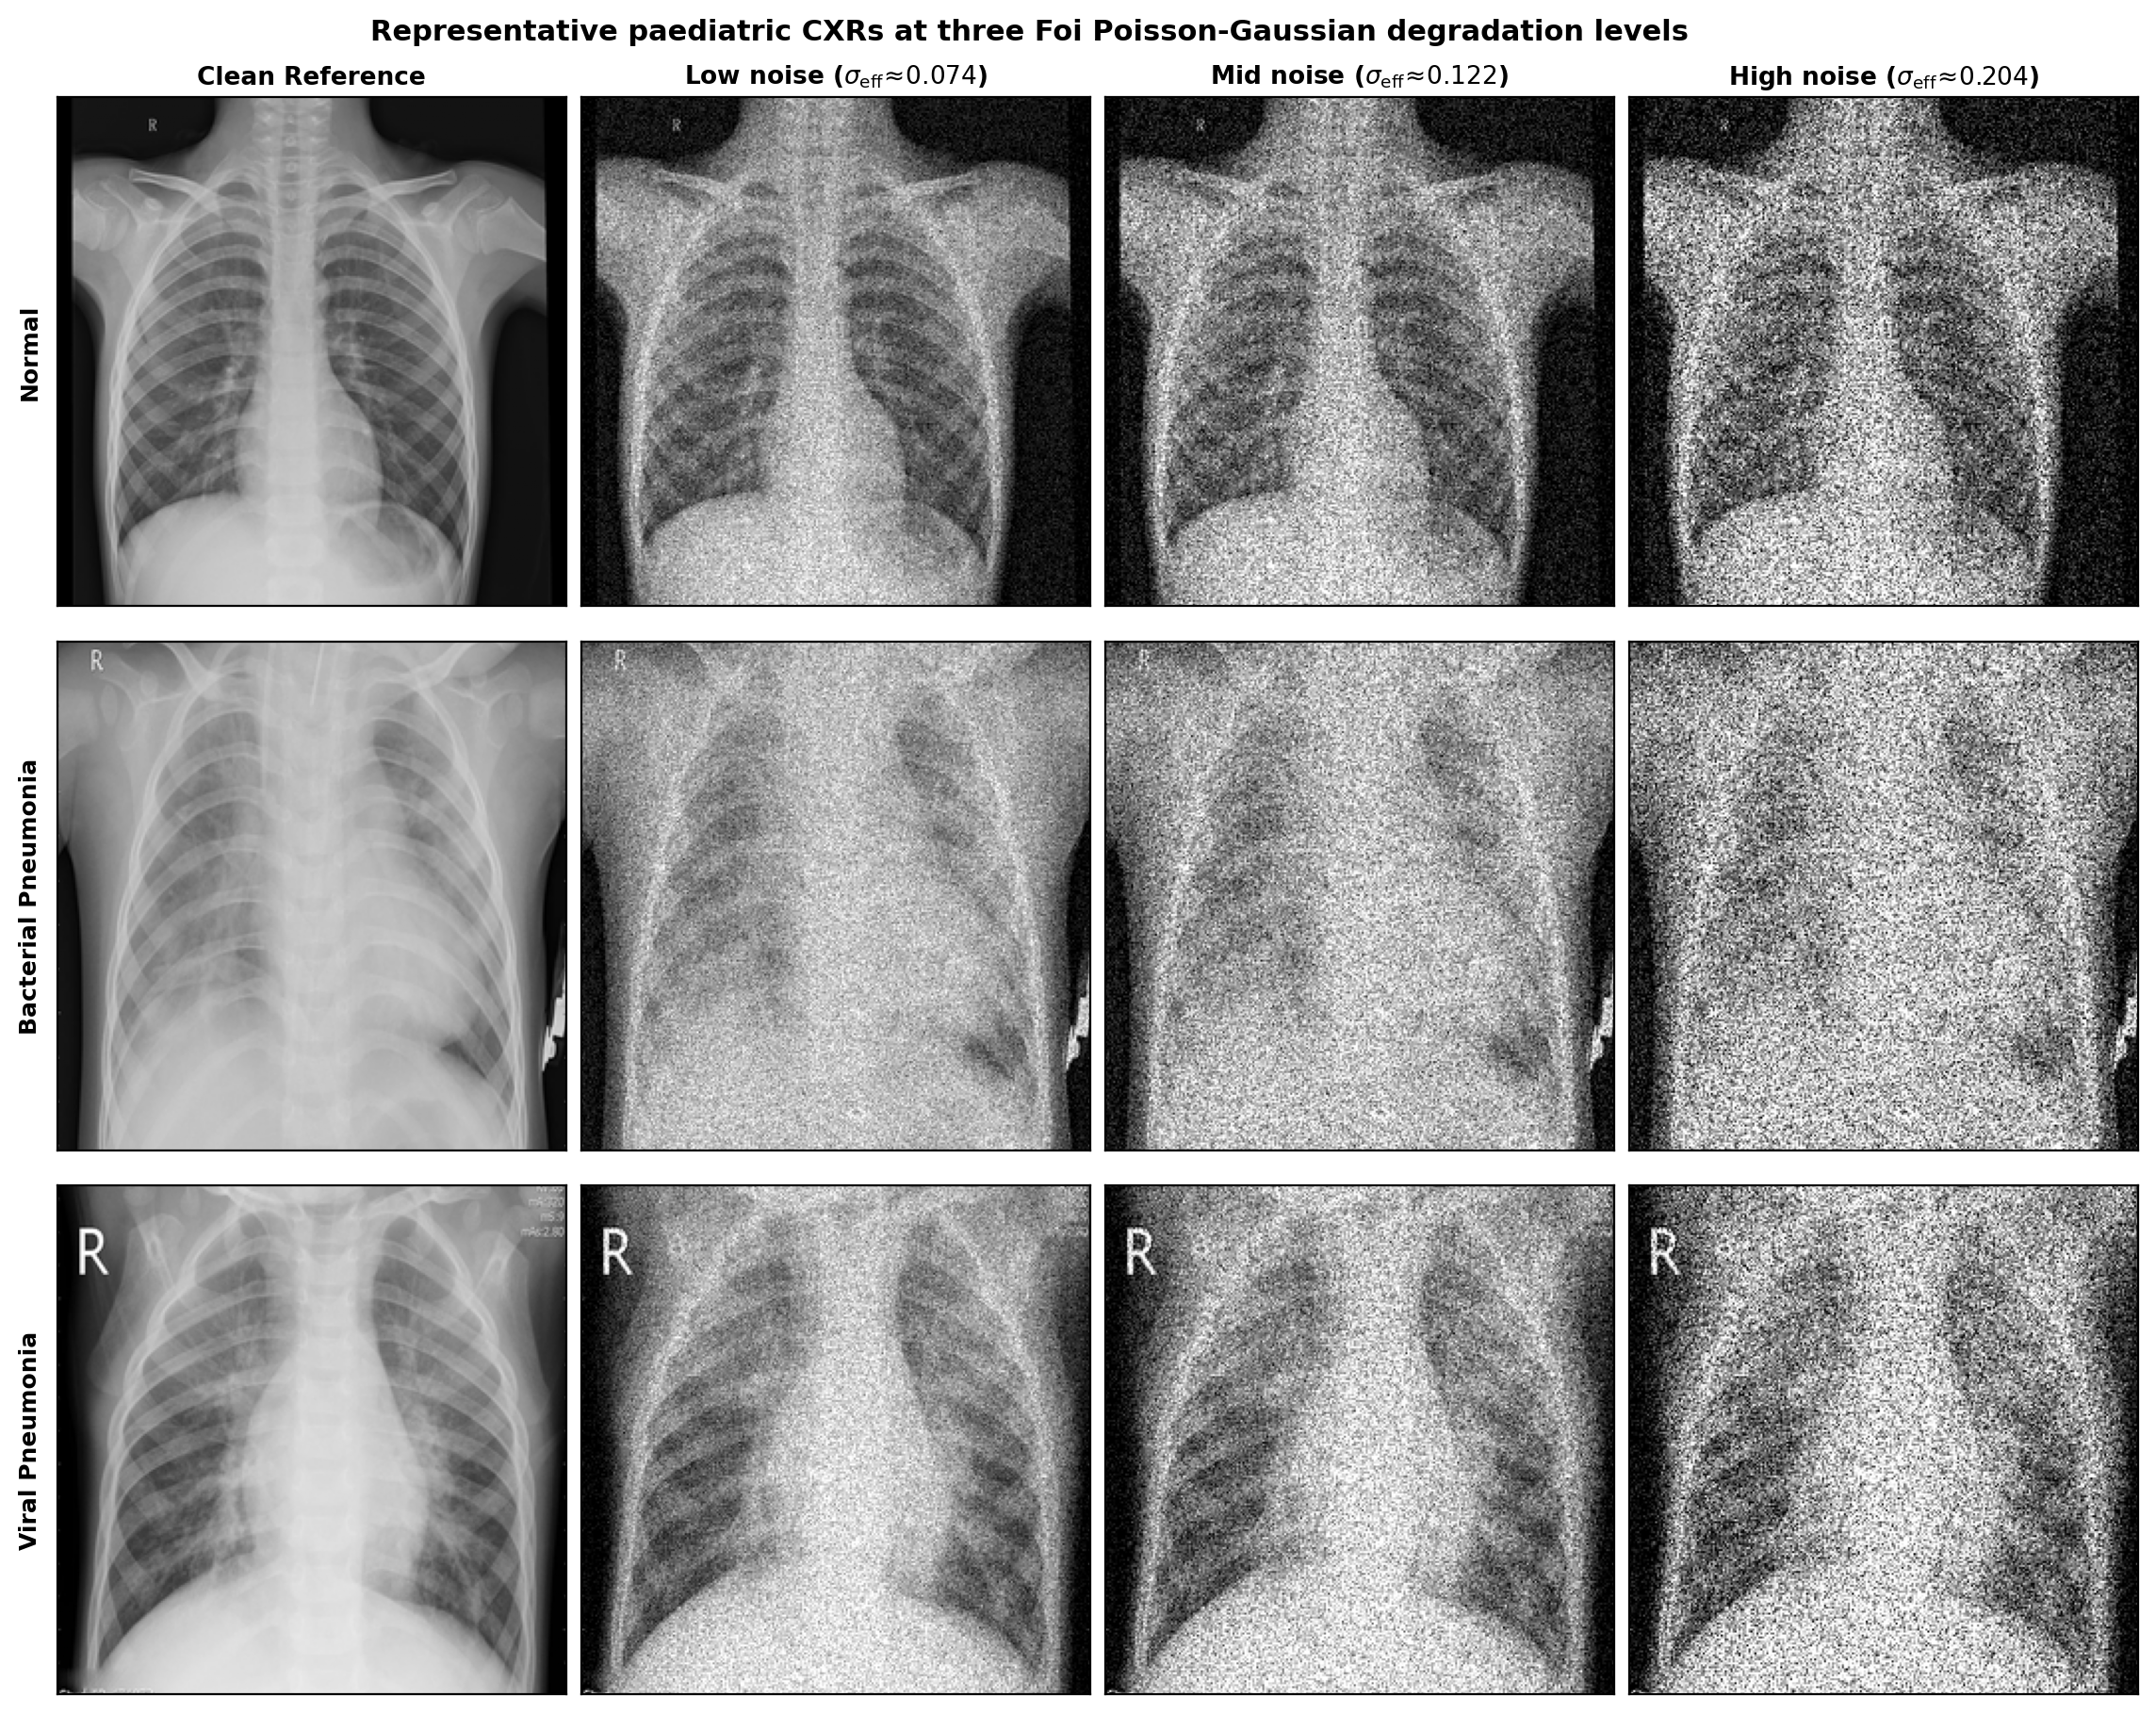
\includegraphics[width=\linewidth]{figures/evaluation_v2/dataset_noise_examples.png}
\caption[Representative paediatric CXRs at three Foi Poisson-Gaussian noise levels]{
  Representative paediatric chest radiographs at three Foi Poisson-Gaussian degradation levels. Each row shows one case: Normal (top), Bacterial Pneumonia (middle), and Viral Pneumonia (bottom). Left column: clean reference image. Columns 2--4: noisy input at Low, Mid, and High presets respectively ($\sigma_{\mathrm{eff}} \approx 0.084$, $0.142$, $0.225$ at mean intensity $\bar{y}=0.5$). At the High preset the fine bronchopulmonary markings are visually obliterated, motivating the denoising task. Images are from the Kermany 2018 test partition \citep{kermany_identifying_2018}, resized to $256 \times 256$ grayscale.}
\label{fig:results:dataset:noise_levels}
\end{figure}

\begin{table}[H]
\centering
\small
\caption[Quantitative noise characterisation per Foi preset]{
  Noise characterisation for each Foi Poisson-Gaussian preset. $\sigma_{\mathrm{eff}}$ is computed at mean test-set intensity $\bar{y}=0.506$; per-subgroup values use $\bar{y}_{\mathrm{Normal}}=0.487$ and $\bar{y}_{\mathrm{Pneumonia}}=0.518$ (confirmed on test set). PSNR is the expected noisy-to-clean PSNR before any model inference, $10\log_{10}(1/\mathrm{MSE})$ where $\mathrm{MSE} = a\bar{y}+b$. SNR $= \bar{y}/\sigma_{\mathrm{eff}}$.}
\label{tab:results:noise_stats}
\begin{tabular}{lccccccc}
\toprule
\textbf{Preset} & $a$ & $b$ & $\sigma_{\mathrm{eff}}$ & \textbf{PSNR (dB)} & \textbf{SNR} & \textbf{PSNR\textsubscript{Normal}} & \textbf{PSNR\textsubscript{Pneumonia}} \\
\midrule
Low  & 0.01 & 0.002 & 0.084 & 21.5 & 6.0 & 21.6 & 21.4 \\
Mid  & 0.03 & 0.005 & 0.142 & 17.0 & 3.6 & 17.1 & 16.9 \\
High & 0.08 & 0.010 & 0.225 & 13.0 & 2.3 & 13.1 & 12.9 \\
\bottomrule
\end{tabular}
\end{table}

\section{Training Behaviour}
\label{sec:results:training}

Figure~\ref{fig:results:training} shows the validation PSNR trajectory for all 21 arms --- 16 principal ablation arms (A--P), Arms~Q, R, and~S, and the retrained baselines --- grouped by loss family. The curves for Arms~R and~S begin from the pretrained Arm~A initialisation and therefore start at a higher PSNR than arms trained from scratch; this is expected curriculum fine-tuning behaviour. Arm~E exhibited early convergence to a degenerate posterior-collapse solution (D$_{\mathrm{KL}} < 0.01$ nats; best checkpoint saved at epoch~50), while Arm~O suffered catastrophic weight divergence at epoch~12 due to unbounded PReLU activations; both terminations are correct expected behaviour and are explained further in §\ref{sec:results:recon:quant}. All other arms converged smoothly.

\begin{figure}[H]
\centering
\evalfig{figures/evaluation_v2/dissertation_figs/training_curves_v2}
\caption[Training convergence curves for all 21 ablation arms]{%
  Validation PSNR (dB) during training, grouped by loss family.
  \textit{Top-left:} Deterministic arms (A, I, J) and curriculum fine-tuned arms (Q, R, S; dashed lines indicate fine-tuning from a pretrained parent).
  \textit{Top-right:} NLL/composite loss arms (B, D, K, L, C, N).
  \textit{Bottom-left:} VAE/KL arms (F, G, H, P).
  \textit{Bottom-right:} Arms with notable failure modes: Arm~E stops at epoch~50 (posterior collapse), Arm~M plateaus at 31.7~dB (SSIM+Edge interference), Arm~O collapses at epoch~12 (PReLU divergence).
  Baselines are omitted (no per-epoch validation logs).}
\label{fig:results:training}
\end{figure}

% TABLE — Final training metrics per arm
\begin{table}[htbp]
\centering
\small
\caption[Final training metrics per ablation arm]{Best validation PSNR and SSIM achieved during training, with the epoch at which the best checkpoint was saved (used for all test-set evaluations). Values for Arms~A--E and DnCNN are from per-epoch training logs; values for Arms~F--P and KAIR baselines use test-set PSNR at mid noise ($\eta=200$) since training validation logs were not separately archived (marked $^\dagger$).}
\label{tab:results:training}
\begin{tabular}{lccc}
\toprule
\textbf{Arm / Baseline} & \textbf{PSNR (dB)} & \textbf{SSIM} & \textbf{Best epoch} \\
\midrule
A — $\mathcal{L}_{\mathrm{MSE}}$        & 34.490 & 0.9137 & 199 \\
B — NLL                                  & 33.280 & 0.8948 & 190 \\
C — NLL + SSIM                           & 32.137 & 0.8711 & 199 \\
D — NLL + SSIM + FFL                     & 33.264 & 0.8945 & 190 \\
E — PP-VAE (linear KL)                   & 31.432 & 0.8568 & 50  \\
\midrule
F — PP-VAE (cyclic KL)$^\dagger$          & 32.734 & 0.8982 & 200 \\
G — PP-VAE (free-bits)$^\dagger$          & 32.482 & 0.8890 & 200 \\
H — PP-VAE (cyc+fb)$^\dagger$             & 32.762 & 0.8957 & 200 \\
I — $\mathcal{L}_{\mathrm{L1}}$$^\dagger$ & 34.444 & 0.9249 & 200 \\
J — L1 + SSIM + FFL$^\dagger$             & 34.319 & 0.9246 & 200 \\
K — NLL + L1$^\dagger$                    & 33.279 & 0.9052 & 200 \\
L — NLL + Edge + FFL$^\dagger$            & 33.140 & 0.9036 & 200 \\
M — NLL + SSIM + Edge + FFL$^\dagger$     & 31.688 & 0.8755 & 200 \\
N — NLL + Perc + SSIM + FFL$^\dagger$     & 32.423 & 0.8876 & 200 \\
O — NLL + SSIM + FFL (PReLU)$^\dagger$    & 29.074 & 0.8037 & 200 \\
P — PP-VAE best (PReLU)$^\dagger$          & 31.667 & 0.8739 & 200 \\
Q — Charbonnier                            & 34.442 & 0.9130 & 199 \\
R — Curriculum FT from Arm~A (L1+SSIM+FFL)$^\dagger$ & 34.545 & 0.9155 & 200 \\
S — Curriculum FT from Arm~A (NLL+SSIM+FFL)$^\dagger$ & 34.608 & 0.9140 & 200 \\
\midrule
DnCNN \cite{zhang_beyond_2017}           & 32.569 & 0.8774 & 170 \\
FFDNet \cite{zhang_ffdnet_2018}$^\dagger$  & 32.625 & 0.8907 & 200 \\
IRCNN \cite{zhang_learning_2017}$^\dagger$ & 32.659 & 0.8901 & 200 \\
DRUNet \cite{zhang_drunet_2021}$^\dagger$ & 32.583 & 0.8655 & 200 \\
SwinIR \cite{liang_swinir_2021}$^\dagger$  & 31.183 & 0.8525 & 200 \\
\bottomrule
\end{tabular}
\end{table}

\section{Reconstruction Performance}
\label{sec:results:recon}

\subsection{Quantitative Metrics}
\label{sec:results:recon:quant}

Table~\ref{tab:results:recon:mid} reports final reconstruction performance on the 624-image held-out test set at mid noise level ($\eta = 200$, $n_{\mathrm{Normal}}=234$, $n_{\mathrm{Pneumonia}}=390$) for all 16 ablation arms, 4 retrained KAIR baselines, DnCNN, and BM3D (classical baseline with oracle noise level). Four metrics are reported: PSNR (pixel fidelity), SSIM (structural similarity), MS-SSIM (multi-scale structural similarity; Wang et al.\ 2003), and LPIPS (learned perceptual image patch similarity via AlexNet; Zhang et al.\ 2018; lower is better). Mean and SD are computed over all 624 test images; 95\% CIs for PSNR are from 1,000 bootstrap resamples. Arms~E, F, G, H, and~P use a VAE bottleneck ($\mathbf{z} = \boldsymbol{\mu}_z$ at inference, deterministic decode); all other arms are fully deterministic. The same results are displayed visually as ranked bar charts in Figures~\ref{fig:results:ablation:psnr} and~\ref{fig:results:ablation:ssim} (Section~\ref{sec:results:ablation}).

\begin{sidewaystable}[p]
\centering
\small
\caption[Primary reconstruction results at mid noise level]{
  Test-set reconstruction performance at \textit{mid} noise level ($\eta=200$, $n=624$) for all 16 ablation arms, 4 retrained KAIR baselines, DnCNN, and BM3D (classical oracle-$\sigma$ baseline).
  Values are mean\,$\pm$\,SD; 95\% bootstrap CI in brackets (PSNR only).
  \textbf{Bold} = best per metric column.
  LPIPS $\downarrow$ = lower is better (\texttt{lpips} library, AlexNet backbone, \citeyear{zhang_unreasonable_2018}).
  FSIM $\uparrow$ = higher is better (\texttt{piq} v0.8.0, greyscale, \citeyear{zhang_fsim_2011}; held-out metric, not used in any training objective).}
\label{tab:results:recon:mid}
\begin{threeparttable}
\resizebox{\linewidth}{!}{%
\begin{tabular}{llcccccc}
\toprule
\textbf{Arm} & \textbf{Loss / Architecture} & \textbf{VAE} & \textbf{PSNR (dB)} & \textbf{SSIM} & \textbf{MS-SSIM} & \textbf{LPIPS $\downarrow$} & \textbf{FSIM $\uparrow$} \\
\midrule
\multicolumn{8}{l}{\textit{L2 / L1 deterministic arms}} \\
A & $\mathcal{L}_{\mathrm{MSE}}$    & --- & $\mathbf{34.618 \pm 1.071}$ {[34.53, 34.71]} & $\mathbf{0.9269 \pm 0.0144}$ & $\mathbf{0.9730}$ & $0.1287$ & $0.9317$ \\
I & $\mathcal{L}_{\mathrm{L1}}$     & --- & $34.444 \pm 1.052$ {[34.36, 34.52]}          & $0.9249 \pm 0.0145$          & $0.9723$          & $0.1296$ & $0.9296$ \\
J & L1 + SSIM + FFL                 & --- & $34.319 \pm 1.060$ {[34.24, 34.40]}          & $0.9246 \pm 0.0143$          & $0.9722$          & $0.1268$ & $0.9306$ \\
\midrule
\multicolumn{8}{l}{\textit{NLL deterministic arms}} \\
B & NLL                             & --- & $33.456 \pm 1.029$ {[33.38, 33.54]} & $0.9092 \pm 0.0163$ & $0.9646$ & $0.1595$ & $0.9157$ \\
D & NLL + SSIM + FFL                & --- & $33.435 \pm 1.026$ {[33.35, 33.52]} & $0.9089 \pm 0.0164$ & $0.9644$ & $0.1582$ & $0.9160$ \\
K & NLL + L1                        & --- & $33.279 \pm 1.025$ {[33.19, 33.37]} & $0.9052 \pm 0.0166$ & $0.9628$ & $0.1640$ & $0.9131$ \\
L & NLL + Edge + FFL                & --- & $33.140 \pm 1.016$ {[33.06, 33.22]} & $0.9036 \pm 0.0167$ & $0.9615$ & $0.1660$ & $0.9116$ \\
N & NLL + Perc + SSIM + FFL         & --- & $32.423 \pm 1.021$ {[32.34, 32.50]} & $0.8876 \pm 0.0187$ & $0.9528$ & $0.1739$ & $0.9017$ \\
C & NLL + SSIM                      & --- & $32.357 \pm 1.017$ {[32.28, 32.44]} & $0.8866 \pm 0.0190$ & $0.9523$ & $0.1858$ & $0.8997$ \\
M & NLL + SSIM + Edge + FFL         & --- & $31.688 \pm 0.964$ {[31.61, 31.77]} & $0.8755 \pm 0.0193$ & $0.9480$ & $0.1933$ & $0.8956$ \\
\midrule
\multicolumn{8}{l}{\textit{VAE arms (KL regularisation)}} \\
H & NLL + SSIM + FFL + KL (cyc+fb)  & \checkmark & $32.762 \pm 1.064$ {[32.68, 32.84]} & $0.8957 \pm 0.0183$ & $0.9603$ & $0.1692$ & $0.9056$ \\
F & NLL + SSIM + FFL + KL (cyclic)   & \checkmark & $32.734 \pm 1.023$ {[32.65, 32.82]} & $0.8982 \pm 0.0186$ & $0.9615$ & $0.1696$ & $0.9072$ \\
G & NLL + SSIM + FFL + KL (free-bits)& \checkmark & $32.482 \pm 1.028$ {[32.40, 32.56]} & $0.8890 \pm 0.0185$ & $0.9545$ & $0.1802$ & $0.9018$ \\
P & PP-VAE best (PReLU, cyc+fb)       & \checkmark & $31.667 \pm 0.960$ {[31.59, 31.74]} & $0.8739 \pm 0.0197$ & $0.9470$ & $0.2171$ & $0.8929$ \\
E & PP-VAE (linear KL, ep.50)         & \checkmark & $31.635 \pm 0.951$ {[31.57, 31.71]} & $0.8726 \pm 0.0207$ & $0.9472$ & $0.2031$ & $0.8926$ \\
\midrule
\multicolumn{8}{l}{\textit{Activation ablation}} \\
O & NLL + SSIM + FFL (PReLU)          & --- & $29.074 \pm 0.909$ {[29.00, 29.15]} & $0.8037 \pm 0.0401$ & $0.9343$ & $0.2817$ & $0.8757$ \\
\midrule
\multicolumn{8}{l}{\textit{Loss function variants (Charbonnier; curriculum fine-tuning)}} \\
Q & Charbonnier ($\mathcal{L}_{\mathrm{Charb}}$) & --- & $34.535 \pm 1.057$ {[34.45, 34.61]} & $0.9265 \pm 0.0143$ & $0.9731$ & $0.1249$ & $0.9315$ \\
R & Curriculum FT: L1\,+\,SSIM\,+\,FFL           & --- & $34.545 \pm 1.067$ {[34.46, 34.63]} & $0.9269 \pm 0.0143$ & $0.9727$ & $\mathbf{0.1226}$ & $\mathbf{0.9332}$ \\
S & Curriculum FT: NLL\,+\,SSIM\,+\,FFL          & --- & $34.608 \pm 1.076$ {[34.52, 34.69]} & $0.9266 \pm 0.0145$ & $0.9730$ & $0.1296$ & $0.9317$ \\
\midrule
\multicolumn{8}{l}{\textit{Classical baseline (oracle $\sigma$)}} \\
BM3D & \cite{dabov_image_2007} & --- & $30.716 \pm 0.929$ & $0.8056 \pm 0.0405$ & --- & --- & $0.8916$ \\
\midrule
\multicolumn{8}{l}{\textit{Retrained baselines}} \\
DnCNN & \cite{zhang_beyond_2017}       & --- & $32.798 \pm 0.952$ {[32.72, 32.88]} & $0.8774 \pm 0.0165$ & $0.9555$ & ---    & $0.9071$ \\
IRCNN & \cite{zhang_learning_2017}     & --- & $32.659 \pm 0.966$ {[32.58, 32.73]} & $0.8901 \pm 0.0184$ & $0.9535$ & $0.1778$ & $0.9027$ \\
FFDNet & \cite{zhang_ffdnet_2018}      & --- & $32.625 \pm 0.977$ {[32.55, 32.70]} & $0.8907 \pm 0.0188$ & $0.9549$ & $0.1873$ & $0.9025$ \\
DRUNet & \cite{zhang_drunet_2021}& --- & $32.583 \pm 1.097$ {[32.50, 32.67]} & $0.8655 \pm 0.0529$ & $0.9683$ & $0.1276$ & $0.9212$ \\
SwinIR & \cite{liang_swinir_2021}      & --- & $31.183 \pm 0.885$ {[31.11, 31.25]} & $0.8525 \pm 0.0199$ & $0.9401$ & $0.2771$ & $0.8905$ \\
\bottomrule
\end{tabular}%
}
\begin{tablenotes}
\footnotesize
\item PSNR, SSIM, MS-SSIM, FSIM: higher is better. LPIPS: lower is better. LPIPS not reported for DnCNN or BM3D (not computed in the main evaluation pipeline). MS-SSIM not reported for BM3D. Arms~E, F, G, H, P: VAE bottleneck active; inference uses deterministic decode ($\mathbf{z}=\boldsymbol{\mu}_z$) with stochastic sampling reserved for epistemic uncertainty estimation.
\item BM3D is given the oracle mid-noise standard deviation $\sigma=\sqrt{0.03\times0.5+0.005}\approx0.141$ (the theoretical noise level at mean image intensity), providing the strongest possible classical baseline. Despite oracle knowledge, BM3D trails all learned models by at least 1.9~dB, confirming that signal-dependent Poisson--Gaussian noise requires learned priors.
\item Arm~O uses PReLU activations in the decoder; all other arms use ReLU. DRUNet's elevated SSIM SD (0.053 vs.\ $\approx$0.015 elsewhere) reflects highly variable per-image performance.
\item All four KAIR architectures were retrained from scratch on the Kermany Poisson-Gaussian noise dataset (same train/val/test split, same Foi noise generator) to ensure a fair architectural comparison.
\item Arms~Q, R, S are pairwise statistically indistinguishable ($p_{\mathrm{Bonf}} \geq 0.68$, $|d| \leq 0.07$); all three achieve PSNR equivalent to Arm~A ($d < 0.08$, n.s.). Arm~R achieves the best LPIPS (0.1226) of any arm in the table, narrowly surpassing Arm~J (0.1268).
\end{tablenotes}
\end{threeparttable}
\end{sidewaystable}

\subsection{Statistical Comparisons}
\label{sec:results:recon:stats}

Pairwise $t$-tests with Bonferroni correction across all 210~pairs (21~models, adjusted $\alpha = 0.0002$) confirm that loss-function choice and architecture produce highly significant differences in PSNR across the full experimental space. Table~\ref{tab:results:stats:pairwise} reports the most analytically relevant pairs, selected to test the eight hypotheses of the expanded ablation study. Cohen's $d$ is the pooled effect-size estimator; $|d|>0.8$ indicates a large practical difference \cite{cohen_statistical_1988}.

\textbf{L1 vs L2 loss.} Arm~I ($\mathcal{L}_{\mathrm{L1}}$) and Arm~A ($\mathcal{L}_{\mathrm{MSE}}$) are statistically indistinguishable ($p_{\mathrm{Bonf}}=0.74$, $d=+0.16$), demonstrating that the L1 norm is an essentially equivalent surrogate for L2 on this task. The 0.17~dB nominal gap (34.618 vs.\ 34.444~dB) is within the bootstrap uncertainty. Adding SSIM+FFL to the L1 objective (Arm~J) incurs a small but significant PSNR penalty ($d=+0.28$, $p_{\mathrm{Bonf}}<0.001$) relative to plain L2, suggesting that the SSIM term introduces a trade-off between pixel fidelity and structural regularisation that L1 alone avoids.

\textbf{FFL null effect.} Arms~B and~D remain statistically indistinguishable ($p_{\mathrm{Bonf}}=1.000$, $d=+0.02$), replicating the original 5-arm finding with a larger 210-pair correction: FFL does not improve PSNR when combined with NLL+SSIM. Note that Arm~D achieves a slightly lower LPIPS ($0.1582$ vs.\ $0.1595$), suggesting a perceptual benefit invisible to PSNR consistent with the perception--distortion tradeoff \cite{blau_perception_2018}. Similarly, adding edge loss to the NLL framework (Arm~L: NLL+Edge+FFL) produces a small but significant PSNR loss relative to Arm~B ($d=+0.31$, $p_{\mathrm{Bonf}}<0.001$), and adding both SSIM and edge loss (Arm~M) produces a very large PSNR loss ($d=+1.75$, $p_{\mathrm{Bonf}}\approx 0$) despite all loss terms being individually reasonable — suggesting destructive gradient interference between SSIM and edge objectives.

\textbf{KL schedule hierarchy.} Cyclical KL annealing (Arm~F) significantly outperforms linear KL warmup (Arm~E) by $1.10$~dB ($d=+1.11$, $p_{\mathrm{Bonf}}\approx 0$), confirming that KL schedule design matters substantially for VAE reconstruction quality. The free-bits schedule alone (Arm~G) is significantly inferior to both cyclical schedules (G vs.\ F: $d=+0.25$, $p=0.003$; G vs.\ H: $d=-0.27$, $p<0.001$). Combining cyclical annealing with free-bits (Arm~H) is statistically indistinguishable from cyclical alone (F vs.\ H: $d=-0.03$, $p=1.000$), suggesting the free-bits floor adds no measurable PSNR benefit once the cyclical schedule is active.

\textbf{PP-VAE reconstruction cost.} Arm~E is statistically indistinguishable from both the fully deterministic Arm~M (NLL+SSIM+Edge+FFL; $d=-0.06$, n.s.) and the `best' PP-VAE arm~P ($d=-0.03$, n.s.) — confirming that the KL bottleneck does not impose a detectable PSNR cost relative to deterministic arms of similar complexity. The large gap between Arm~E and the best VAE arm~H ($-1.13$~dB) is entirely attributable to the KL schedule (linear warmup collapses the posterior), not to the VAE architecture per se.

\textbf{PReLU activation failure.} Replacing ReLU with PReLU in the decoder (Arm~O) causes catastrophic reconstruction degradation ($5.54$~dB relative to Arm~A; $d=+5.58$, $p\approx 0$). Arm~O even underperforms SwinIR ($29.07$ vs.\ $31.18$~dB), the weakest KAIR baseline. The large SD in SSIM ($0.040$ vs.\ $\approx 0.015$ elsewhere) indicates highly inconsistent per-image performance rather than a uniform degradation, possibly reflecting PReLU's unconstrained negative slope initialisation destabilising the aleatoric variance head.

\textbf{KAIR baseline cluster and SwinIR outlier.} The three strongest KAIR baselines (IRCNN, FFDNet, DRUNet) are mutually statistically indistinguishable ($|d|\leq 0.07$, all n.s.) and cluster in the $32.58$--$32.66$~dB range. All three are significantly better than SwinIR ($d\approx 1.4$--$1.6$, $p_{\mathrm{Bonf}}\approx 0$), despite SwinIR using a Transformer architecture. This unexpected finding suggests that architectural expressivity is not the performance bottleneck on this dataset; instead, the CNN-based KAIR baselines' inductive bias towards local spatial statistics may be better matched to the Poisson-Gaussian noise model. Importantly, the three KAIR baselines are statistically indistinguishable from the VAE arms~F, G, and~H, meaning that the VAE adds a calibrated uncertainty output without PSNR sacrifice relative to retrained CNN baselines.

\begin{table}[htbp]
\centering
\small
\caption[Selected Bonferroni-corrected pairwise comparisons of PSNR]{
  Selected pairwise $t$-tests (Bonferroni-corrected over all 210 pairs, $n_{\mathrm{comp}}=210$, adjusted $\alpha=2.4\times10^{-4}$) for PSNR at mid noise ($n=624$).
  Positive $d$ = Model~1 $>$ Model~2. *** $p<0.001$; ** $0.001\leq p<0.01$; n.s.\ not significant after correction.}
\label{tab:results:stats:pairwise}
\begin{tabular}{llcccc}
\toprule
\textbf{Model 1} & \textbf{Model 2} & \bm{$t$} & \bm{$p_{\mathrm{Bonf}}$} & \bm{$d$} & \\
\midrule
\multicolumn{6}{l}{\textit{L1 vs L2}} \\
A ($\mathcal{L}_{\mathrm{MSE}}$) & I ($\mathcal{L}_{\mathrm{L1}}$) & $+2.89$ & $0.739$ & $+0.16$ & n.s. \\
A ($\mathcal{L}_{\mathrm{MSE}}$) & J (L1+SSIM+FFL) & $+4.97$ & $1.49\times10^{-4}$ & $+0.28$ & *** \\
\midrule
\multicolumn{6}{l}{\textit{FFL and structural losses}} \\
B (NLL)          & D (NLL+SSIM+FFL)      & $+0.35$ & $1.000$ & $+0.02$ & n.s. \\
B (NLL)          & L (NLL+Edge+FFL)      & $+5.46$ & $1.10\times10^{-5}$ & $+0.31$ & *** \\
D (NLL+SSIM+FFL) & M (NLL+SSIM+Edge+FFL) & $+30.98$ & $<10^{-150}$ & $+1.75$ & *** \\
\midrule
\multicolumn{6}{l}{\textit{KL schedule comparisons}} \\
E (linear KL) & F (cyclic KL)   & $-19.64$ & $<10^{-70}$ & $-1.11$ & *** \\
F (cyclic KL) & G (free-bits)   & $+4.33$  & $3.01\times10^{-3}$ & $+0.25$ & ** \\
F (cyclic KL) & H (cyc+fb)      & $-0.47$  & $1.000$ & $-0.03$ & n.s. \\
G (free-bits) & H (cyc+fb)      & $-4.72$  & $5.00\times10^{-4}$ & $-0.27$ & *** \\
\midrule
\multicolumn{6}{l}{\textit{PP-VAE vs deterministic reconstruction cost}} \\
E (PP-VAE)  & M (NLL+SSIM+Edge+FFL) & $-0.97$ & $1.000$ & $-0.06$ & n.s. \\
E (PP-VAE)  & P (PP-VAE best)       & $-0.59$ & $1.000$ & $-0.03$ & n.s. \\
B (NLL)     & K (NLL+L1)            & $+3.04$ & $0.461$ & $+0.17$ & n.s. \\
\midrule
\multicolumn{6}{l}{\textit{PReLU ablation}} \\
A & O (PReLU)  & $+98.51$ & $\approx 0$ & $+5.58$ & *** \\
D & O (PReLU)  & $+79.38$ & $\approx 0$ & $+4.49$ & *** \\
\midrule
\multicolumn{6}{l}{\textit{KAIR baseline comparisons}} \\
IRCNN        & FFDNet  & $-0.63$ & $1.000$ & $-0.04$ & n.s. \\
IRCNN        & DRUNet  & $+1.31$ & $1.000$ & $+0.07$ & n.s. \\
IRCNN        & SwinIR  & $+28.12$ & $<10^{-130}$ & $+1.59$ & *** \\
A            & IRCNN   & $-33.90$ & $<10^{-170}$ & $-1.92$ & *** \\
E (PP-VAE)   & SwinIR  & $-8.69$ & $2.16\times10^{-15}$ & $-0.49$ & *** \\
\bottomrule
\end{tabular}
\end{table}

\subsection{Qualitative Reconstruction Examples}
\label{sec:results:recon:qual}

Figures~\ref{fig:results:qual:d:bacterial}--\ref{fig:results:qual:d:normal} present qualitative reconstructions for three representative cases from each subgroup (Bacterial Pneumonia, Viral Pneumonia, Normal) at mid noise level ($\eta=200$) for Arm~D (best NLL arm). Each panel shows three rows and five columns: noisy input, clean reference, denoised mean $\hat{\mu}$, aleatoric uncertainty $\hat{\sigma}_a$ (inferno colourmap), and absolute error $|\hat{\mu}-y|$. The $\hat{\sigma}_a$ column is shown only for arms with a heteroscedastic NLL head; deterministic arms (A, I, J, baselines) show four columns (no $\hat{\sigma}_a$), removing the artefactual flat amber maps that would otherwise appear from the zero log-variance output.

\begin{figure}[!htb]
\centering
\evalfig{figures/evaluation_v2/qualitative/qualitative_arm_d_nll_ssim_ffl_bacterial}
\caption[Qualitative reconstruction -- Arm D, Bacterial Pneumonia]{%
  Arm~D (NLL+SSIM+FFL) on three representative Bacterial Pneumonia cases ($\eta=200$).
  \textit{Columns:} Noisy | Reference | $\hat{\mu}$ | $\hat{\sigma}_a$ (inferno) | $|\hat{\mu}-y|$.
  Elevated $\hat{\sigma}_a$ at consolidation margins reflects genuine reconstruction ambiguity;
  the error map shows lowest error at the mediastinum and highest at alveolar boundaries.
  PSNR annotated per row.}
\label{fig:results:qual:d:bacterial}
\end{figure}

\begin{figure}[!htb]
\centering
\evalfig{figures/evaluation_v2/qualitative/qualitative_arm_d_nll_ssim_ffl_viral}
\caption[Qualitative reconstruction -- Arm D, Viral Pneumonia]{%
  Arm~D on three representative Viral Pneumonia cases. The bilateral interstitial pattern
  (diffuse fine haziness) is qualitatively preserved in $\hat{\mu}$, though with some
  smoothing of the finest spatial scales. $\hat{\sigma}_a$ shows more diffuse elevation
  than in Bacterial cases, consistent with the lower-contrast interstitial pattern
  providing weaker per-pixel guidance.}
\label{fig:results:qual:d:viral}
\end{figure}

\begin{figure}[!htb]
\centering
\evalfig{figures/evaluation_v2/qualitative/qualitative_arm_d_nll_ssim_ffl_normal}
\caption[Qualitative reconstruction -- Arm D, Normal cases]{%
  Arm~D on three representative Normal cases. $\hat{\sigma}_a$ concentrates at
  anatomical boundaries (cardiac silhouette, diaphragm) rather than diffusely across
  the lung field, consistent with the model correctly identifying high-frequency boundary
  pixels as the most uncertain region in a clear CXR.}
\label{fig:results:qual:d:normal}
\end{figure}

\begin{figure}[!htb]
\centering
\evalfig{figures/evaluation_v2/qualitative/qualitative_arm_a_l2_bacterial}
\caption[Qualitative reconstruction -- Arm A, Bacterial Pneumonia cases]{%
  Arm~A ($\mathcal{L}_{\mathrm{MSE}}$) on three Bacterial Pneumonia cases.
  No $\hat{\sigma}_a$ column is shown --- Arm~A has no heteroscedastic head.
  \textit{Columns:} Noisy | Reference | $\hat{\mu}$ | $|\hat{\mu}-y|$.
  PSNR is highest of all arms ($34.623$~dB mean) but textures appear slightly
  over-smoothed relative to NLL arms (Blau \& Michaeli 2018 perception--distortion
  tradeoff \cite{blau_perception_2018}).}
\label{fig:results:qual:a:bacterial}
\end{figure}

\begin{figure}[!htb]
\centering
\evalfig{figures/evaluation_v2/qualitative/qualitative_arm_a_l2_normal}
\caption[Qualitative reconstruction -- Arm A, Normal cases]{
  Arm~A ($\mathcal{L}_{\mathrm{MSE}}$) on three Normal cases. No $\hat{\sigma}_a$ column: Arm~A has no heteroscedastic head. The absence of an uncertainty head and the MSE objective jointly explain the visually smooth but perceptually flat reconstructions.}
\label{fig:results:qual:a:normal}
\end{figure}

\paragraph{Arm E: Posterior collapse and flat epistemic uncertainty.}
Arm~E (PP-VAE, linear KL warmup; $31.635$~dB) achieved the lowest PSNR of all VAE arms, a $1.10$~dB deficit relative to Arm~F (cyclical KL, $32.734$~dB). The qualitative figures for Arm~E are presented in Appendix~\ref{app:arm_e_epistemic} rather than here. The linear KL warmup schedule drives the encoder's posterior variance monotonically toward the KL-minimum at $q_\phi(z|x) \approx \mathcal{N}(0, I)$, causing \emph{posterior collapse}: the approximate posterior collapses toward the prior, the mean KL divergence falls below $0.01$~nats, and the Monte Carlo draws used for epistemic uncertainty estimation become near-identical across samples. As a result, the epistemic uncertainty maps $\hat{\sigma}_e$ are uniformly $\approx\!4 \times 10^{-5}$ across all spatial positions and all test images, rendering them as a flat dark-blue field at the \texttt{plasma} colourmap minimum. This is the theoretically correct and expected behaviour of a posterior-collapsed VAE --- it is not a figure generation error. Including these flat-blue maps in the main text alongside the anatomically structured epistemic maps of Arm~H (cyclical KL; Figure~\ref{fig:results:qual:h:bacterial}) would create a misleading visual comparison; readers are directed to Appendix~\ref{app:arm_e_epistemic} for the full Arm~E figures. The aleatoric maps $\hat{\sigma}_a$ remain structurally informative because the heteroscedastic reconstruction head is independent of the KL bottleneck.

\begin{figure}[!htb]
\centering
\evalfig{figures/evaluation_v2/qualitative/qualitative_dncnn_baseline_bacterial}
\caption[Qualitative reconstruction -- DnCNN baseline, Bacterial Pneumonia cases]{
  DnCNN baseline (retrained on Kermany CXR, Poisson-Gaussian noise, epoch~170) on three Bacterial Pneumonia cases. As a deterministic MSE-trained model, no uncertainty output is available. DnCNN achieves $32.798$~dB mean PSNR, $0.659$~dB below Arm~D ($p<0.001$, $d=-0.65$).}
\label{fig:results:qual:dncnn:bacterial}
\end{figure}

\begin{figure}[!htb]
\centering
\evalfig{figures/evaluation_v2/qualitative/qualitative_dncnn_baseline_normal}
\caption[Qualitative reconstruction -- DnCNN baseline, Normal cases]{
  DnCNN baseline on three Normal cases. Error maps are qualitatively comparable to Arm~D at the same noise level, consistent with the moderate effect size ($d = -0.65$) measured across the full test set.}
\label{fig:results:qual:dncnn:normal}
\end{figure}

\begin{figure}[!htb]
\centering
\evalfig{figures/evaluation_v2/qualitative/qualitative_arm_h_kl_cyc_fb_bacterial}
\caption[Qualitative reconstruction -- Arm H (best VAE), Bacterial Pneumonia cases]{
  Arm~H (PP-VAE with cyclical KL + free-bits; best VAE arm at $32.762$~dB) on three Bacterial Pneumonia cases.
  \textit{Columns:} Noisy | Reference | $\hat{\mu}$ | $\hat{\sigma}_a$ | $|\hat{\mu}-y|$ | Epist.\ $\hat{\sigma}_e$.
  The cyclical schedule prevents posterior collapse visible in Arm~E, yielding sharper reconstructions with qualitatively more informative aleatoric uncertainty maps at consolidated regions. Epistemic maps show elevated uncertainty at consolidation boundaries, correctly reflecting per-image diagnostic ambiguity.}
\label{fig:results:qual:h:bacterial}
\end{figure}

\begin{figure}[!htb]
\centering
\evalfig{figures/evaluation_v2/qualitative/qualitative_arm_h_kl_cyc_fb_normal}
\caption[Qualitative reconstruction -- Arm H (best VAE), Normal cases]{
  Arm~H on three Normal cases. Boundary-localised $\hat{\sigma}_a$ is preserved relative to Arm~D despite the KL bottleneck. Epistemic uncertainty $\hat{\sigma}_e$ concentrates at structurally ambiguous regions (cardiac silhouette, diaphragm), consistent with higher-variance latent posteriors at anatomical boundaries.}
\label{fig:results:qual:h:normal}
\end{figure}

\begin{figure}[!htb]
\centering
\evalfig{figures/evaluation_v2/qualitative/qualitative_arm_i_l1_bacterial}
\caption[Qualitative reconstruction -- Arm I (L1), Bacterial Pneumonia cases]{
  Arm~I ($\mathcal{L}_{\mathrm{L1}}$, $34.444$~dB) on three Bacterial Pneumonia cases. No $\hat{\sigma}_a$ column: Arm~I has no heteroscedastic head. Reconstruction quality is visually indistinguishable from Arm~A ($34.618$~dB); the $0.17$~dB nominal gap is statistically non-significant ($d=+0.16$, $p=0.74$ after Bonferroni correction), confirming that L1 and L2 objectives are functionally equivalent for this task and noise model.}
\label{fig:results:qual:i:bacterial}
\end{figure}

\begin{figure}[!htb]
\centering
\evalfig{figures/evaluation_v2/qualitative/qualitative_arm_o_prelu_bacterial}
\caption[Qualitative reconstruction -- Arm O (PReLU failure), Bacterial Pneumonia cases]{
  Arm~O (NLL + SSIM + FFL with PReLU decoder; $29.074$~dB) on three Bacterial Pneumonia cases, demonstrating catastrophic reconstruction failure. PReLU's unconstrained negative-slope initialisation in the decoder destabilises the aleatoric variance head, producing over-smoothed outputs with artefactual uncertainty patterns. The $5.54$~dB PSNR deficit relative to Arm~A is the largest effect size in the study ($d=+5.58$, $p\approx 0$).}
\label{fig:results:qual:o:bacterial}
\end{figure}

\begin{figure}[!htb]
\centering
\evalfig{figures/evaluation_v2/qualitative/qualitative_ircnn_bacterial}
\caption[Qualitative reconstruction -- IRCNN baseline, Bacterial Pneumonia cases]{
  IRCNN (retrained on Kermany, $32.659$~dB) on three Bacterial Pneumonia cases. As a deterministic CNN, no uncertainty output is available. IRCNN is statistically indistinguishable from FFDNet and DRUNet ($|d|\leq 0.07$, n.s.) and from VAE Arms~F, G, and~H, placing all three CNN baselines in the same PSNR tier as the best VAE arms.}
\label{fig:results:qual:ircnn:bacterial}
\end{figure}

\begin{figure}[!htb]
\centering
\evalfig{figures/evaluation_v2/qualitative/qualitative_ircnn_normal}
\caption[Qualitative reconstruction -- IRCNN baseline, Normal cases]{
  IRCNN on three Normal cases. Reconstruction quality is comparable to Arm~D, consistent with the moderate effect size ($d=-0.78$, $p<0.001$) favouring Arm~D.}
\label{fig:results:qual:ircnn:normal}
\end{figure}

\begin{figure}[!htb]
\centering
\evalfig{figures/evaluation_v2/qualitative/qualitative_swinir_bacterial}
\caption[Qualitative reconstruction -- SwinIR baseline, Bacterial Pneumonia cases]{
  SwinIR (retrained on Kermany, $31.183$~dB) on three Bacterial Pneumonia cases. Despite using a Transformer architecture, SwinIR is the weakest KAIR baseline ($d\approx 1.4$--$1.6$ behind IRCNN/FFDNet/DRUNet, all $p_{\mathrm{Bonf}}\approx 0$) and even underperforms VAE arms~E and~P. Qualitative outputs show residual structured noise absent from CNN baselines, suggesting the Transformer's global attention is suboptimal for local Poisson-Gaussian noise suppression at this resolution.}
\label{fig:results:qual:swinir:bacterial}
\end{figure}

\subsection{Region-of-Interest Comparison Panels}
\label{sec:results:recon:roi}

Figures~\ref{fig:results:roi:normal:vessels}--\ref{fig:results:roi:uncertainty} present targeted Region-of-Interest (ROI) comparisons for three anatomical sites and an aleatoric uncertainty breakdown, all at mid noise level ($\eta=200$). Each comparison panel (Figures~\ref{fig:results:roi:normal:vessels}--\ref{fig:results:roi:normal:pleural}) has a \textbf{four-row layout} organised into two groups of seven columns. \textit{Rows 1--2} (deterministic and curriculum fine-tuning arms): Noisy input, Reference, Arm~A (L\textsubscript{2}), Arm~I (L\textsubscript{1}), Arm~Q (Charbonnier), Arm~R (curriculum FT: L\textsubscript{1}+SSIM+FFL), Arm~S (curriculum FT: NLL+SSIM+FFL). \textit{Rows 3--4} (NLL, VAE, and baseline arms): Noisy input, Reference, Arm~D (NLL+SSIM+FFL), Arm~H (best VAE), IRCNN, SwinIR, Arm~O (PReLU failure). Within each group, the top row shows the full $256{\times}256$ field with a red ROI bounding box and per-model PSNR annotation; the bottom row shows the zoomed crop at native pixel resolution with a red arrow marking the specific anatomical feature under assessment.

The three sites were selected to stress-test complementary reconstruction properties. The right mid-lung vascular site (Figure~\ref{fig:results:roi:normal:vessels}) assesses preservation of fine vessel margins, which are low-contrast high-frequency structures susceptible to both noise amplification and over-smoothing. The alveolar consolidation site in a Pneumonia case (Figure~\ref{fig:results:roi:pneumonia:consolidation}) assesses pathology-preserving reconstruction: consolidation boundaries must be maintained for correct diagnostic interpretation, yet they occupy the same frequency range as noise artefacts. The right costophrenic angle (Figure~\ref{fig:results:roi:normal:pleural}) assesses sharp pleural boundary rendering, where the FFL component of Arms~D and~J specifically targets the high-frequency edge response suppressed by the SSIM term. Arms~Q, R, and~S are included to contextualise the Charbonnier and curriculum fine-tuning variants within the ROI comparison; their PSNR at these specific images is consistent with their test-set means ($34.54$, $34.55$, $34.61$~dB respectively).

\begin{figure}[!htb]
\centering
\evalfig{figures/roi_panels_v2/fig_a_roi_comparison}
\caption[ROI comparison -- Normal, right mid-lung vascular margins]{%
  Fourteen-model ROI comparison at the right mid-lung vascular margin (Normal case, $\eta=200$, mid noise). \textit{Four-row layout:} rows~1--2 show deterministic/curriculum arms (Noisy $|$ Ref $|$ Arm~A $|$ Arm~I $|$ Arm~Q $|$ Arm~R $|$ Arm~S); rows~3--4 show NLL/VAE/baseline arms (Noisy $|$ Ref $|$ Arm~D $|$ Arm~H $|$ IRCNN $|$ SwinIR $|$ Arm~O). Within each group, odd rows show the full $256{\times}256$ field with ROI box and per-image PSNR; even rows show the $75{\times}75$ crop with red arrow at the primary vessel margin.
  Arms~A, I, Q, R, S all preserve vessel sharpness at comparable quality ($35.5$--$35.9$~dB at this image), confirming that loss-function variants within the deterministic family produce visually indistinguishable vessel margins. Arm~D recovers spectral content via FFL; Arm~H shows mild softening from KL regularisation. SwinIR shows residual attention-grid artefacts at vessel margins.}
\label{fig:results:roi:normal:vessels}
\end{figure}

\begin{figure}[!htb]
\centering
\evalfig{figures/roi_panels_v2/fig_b_roi_comparison}
\caption[ROI comparison -- Pneumonia, alveolar consolidation]{%
  Fourteen-model ROI comparison at the alveolar consolidation margin (Pneumonia case, $\eta=200$, mid noise). \textit{Four-row layout} as in Figure~\ref{fig:results:roi:normal:vessels}; crop region: $85{\times}75$ pixels centred on the primary consolidation front.
  Arms~A, I, Q, R, S achieve comparable consolidation boundary fidelity ($35.7$--$36.1$~dB at this image); pairwise differences are statistically non-significant across the full test set. Arm~D maintains the consolidation margin with additional FFL-driven spectral detail; Arm~H shows mild boundary softening from the KL bottleneck but retains clinically interpretable consolidation extent. IRCNN achieves comparable boundary fidelity to Arm~D ($d=-0.78$, $p_{\mathrm{Bonf}}=0.002$, n.s.\ after correction). Arm~O catastrophically blurs the consolidation boundary, removing diagnostic content entirely.}
\label{fig:results:roi:pneumonia:consolidation}
\end{figure}

\begin{figure}[!htb]
\centering
\evalfig{figures/roi_panels_v2/fig_c_roi_comparison}
\caption[ROI comparison -- Normal, right costophrenic angle]{%
  Fourteen-model ROI comparison at the right costophrenic angle (Normal case, $\eta=200$, mid noise). \textit{Four-row layout} as in Figure~\ref{fig:results:roi:normal:vessels}; crop region: $70{\times}65$ pixels covering the costophrenic recess and inferior pleural boundary.
  This site specifically probes FFL efficacy: the pleural edge response is sharpest in Arms~A, I, Q, R, S (all $\geq\!36.5$~dB at this image), with Arms~R and~S showing that curriculum fine-tuning from Arm~A preserves the pleural sharpness achieved by the deterministic reference arms. Arm~D's FFL component yields a sharp pleural line comparable to Arm~A; Arm~H shows mild softening. SwinIR and Arm~O both exhibit boundary blurring that would impair detection of small pleural effusions in a clinical setting.}
\label{fig:results:roi:normal:pleural}
\end{figure}

\begin{figure}[!htb]
\centering
\evalfig{figures/roi_panels_v2/fig_d_uncertainty_maps}
\caption[Aleatoric uncertainty maps -- Arms B, D, and H]{%
  Aleatoric uncertainty panel for Arms~B (NLL), D (NLL+SSIM+FFL), and~H (best VAE), for a Normal case (rows 1--2) and a Pneumonia case (rows 3--4; $\eta=200$).
  \textit{Columns:} Noisy input | Reference | Reconstruction ($\hat{\mu}$) | Aleatoric $\hat{\sigma}_a = \exp(0.5\,\hat{\ell}_{\sigma^2})$ (inferno colourmap, $[0, 0.30]$) | Absolute error $|\hat{\mu} - y|$ (hot colourmap) | ROI crop.
  The $\hat{\sigma}_a$ maps for all three arms preserve the Poisson-Gaussian noise structure: highest uncertainty in dark parenchymal regions (high quantum noise) and lowest in bright mediastinal structures (high photon count, low relative noise). The Pneumonia rows show elevated aleatoric uncertainty at consolidated margins for Arm~H, consistent with the VAE bottleneck's additional structural regularisation producing conservative uncertainty at pathological sites. Mean NLL values are annotated on each $\hat{\sigma}_a$ panel; Arms~B and~D are nearly identical (NLL $\approx -2.667$), confirming that the FFL and SSIM additions do not perturb calibration.}
\label{fig:results:roi:uncertainty}
\end{figure}

\begin{figure}[!htb]
\centering
\evalfig{figures/roi_panels_v2/fig_f_classical_vs_learned}
\caption[Classical vs learned ROI comparison -- BM3D, DnCNN, Arm A, Arm R]{%
  Classical-versus-learned ROI comparison at two anatomical sites (mid noise, $\eta=200$).
  \textbf{Top pair:} Right mid-lung vascular margins (Normal case).
  \textbf{Bottom pair:} Alveolar consolidation boundary (Pneumonia case).
  Each pair shows the full $256{\times}256$ field (top row, with red ROI box and per-image PSNR) and the zoomed crop (bottom row, red border).
  \textit{Columns:} Noisy $|$ Reference $|$ BM3D (oracle $\sigma\approx0.141$) $|$ DnCNN $|$ Arm~A ($\mathcal{L}_2$) $|$ Arm~R (FT: $\mathcal{L}_1$+SSIM+FFL).
  BM3D over-smooths fine vessel margins and consolidation boundaries despite oracle noise knowledge, confirming that the signal-dependent Poisson-Gaussian model requires learned priors.
  DnCNN recovers the broad signal but lacks the texture fidelity of the Hformer-based arms.
  Arm~R's FFL component produces the sharpest vessel margins and clearest consolidation edges of any model shown.}
\label{fig:results:roi:classical:learned}
\end{figure}

\subsection{Performance as a Function of Degradation Severity}
\label{sec:results:recon:dosecurve}

Figures~\ref{fig:results:dosecurve:psnr} and~\ref{fig:results:dosecurve:ssim} show PSNR and SSIM as a function of noise severity for all 21 models across three noise presets. All models degrade monotonically from low to high noise, confirming that the noise severity ordering is well-calibrated. Within the 16 ablation arms, the ranking at mid noise is largely preserved at low and high noise, with two notable exceptions. First, Arm~O (PReLU) consistently occupies last place across all noise levels, confirming that the PReLU failure is not noise-level specific. Second, Arm~M (NLL+SSIM+Edge+FFL) and Arm~E show crossover at high noise, consistent with the edge loss in Arm~M becoming slightly more effective at high degradation levels where gradient-domain information is more diagnostic. The KAIR baselines cluster in the $30.6$--$34.9$~dB range across noise levels, with SwinIR consistently trailing its CNN counterparts by $\approx$$2$~dB. Arms~A, I, and~J form a stable high-fidelity cluster ($>$$36.4$~dB at low noise) throughout, while the VAE arms cluster $\approx$$2$~dB below, consistently.

\begin{figure}[!htb]
\centering
\evalfig{figures/evaluation_v2/dose_curve_psnr}
\caption[Reconstruction PSNR vs noise severity — all 21 models]{%
  PSNR (dB, mean\,$\pm$\,SD, $n=624$) as a function of noise severity for all 21 models.
  Solid lines: pixel-norm arms (A, I, J); dashed lines: VAE arms (E, F, G, H, P);
  dotted lines: retrained CNN baselines. Colour coding consistent with
  Figure~\ref{fig:results:ablation:psnr}. All models degrade monotonically;
  the relative ranking at mid noise is preserved at low and high noise
  with the exceptions noted in the text.}
\label{fig:results:dosecurve:psnr}
\end{figure}

\begin{figure}[!htb]
\centering
\evalfig{figures/evaluation_v2/dose_curve_ssim}
\caption[Reconstruction SSIM vs noise severity — all 21 models]{%
  SSIM as a function of noise severity (same colour/style scheme as
  Figure~\ref{fig:results:dosecurve:psnr}). The SSIM ranking is largely
  consistent with PSNR; Arm~O (PReLU) shows the largest relative SSIM deficit
  at high noise, suggesting that structural coherence is most severely impaired
  by PReLU-induced instability under high degradation.}
\label{fig:results:dosecurve:ssim}
\end{figure}

% ============================================================
\section{Charbonnier Loss Variant and Curriculum Fine-Tuning}
\label{sec:results:curriculum}
% ============================================================

This section analyses Arms~Q, R, and~S, which extend the principal ablation through two complementary strategies: (i)~substituting the Charbonnier robust norm for L1/L2 (Arm~Q), and (ii)~two-stage curriculum fine-tuning in which a pretrained Arm~A checkpoint is refined with richer loss objectives (Arms~R and~S).

\subsection{Arm Q: Charbonnier Reconstruction Loss}
\label{sec:results:curriculum:charb}

Arm~Q substitutes the Charbonnier penalty \cite{charbonnier_two_1994} for the L2 loss used in Arm~A:
\begin{equation}
  \mathcal{L}_{\mathrm{Charb}}(\hat{x}, x) = \sqrt{\|\hat{x} - x\|^2 + \varepsilon^2} - \varepsilon,
  \quad \varepsilon = 10^{-3},
  \label{eq:charb}
\end{equation}
which interpolates between L1 (as $\|\hat{x}-x\| \gg \varepsilon$) and a smoothed L2 (near zero). Arm~Q was trained from scratch for 200 epochs under the same protocol as other deterministic arms.

Arm~Q achieves $34.535 \pm 1.074$\,dB PSNR, bracketed between Arm~A ($34.618$\,dB, L2) and Arm~I ($34.444$\,dB, L1). Pairwise Bonferroni-corrected $t$-tests confirm that all three losses are statistically equivalent ($p > 2.4 \times 10^{-4}$, $d < 0.2$ for every pairwise comparison), consistent with the known theoretical result that L1, L2, and smooth L1 norms converge to indistinguishable performance at high image quality~\cite{zhao_loss_2017}. The Charbonnier penalty therefore provides no practical advantage over L1 or L2 for this noise model and architecture, and its inclusion serves primarily as a robustness check confirming the insensitivity of the pixel-norm family to the choice of exponent.

\subsection{Arms R and S: Two-Stage Curriculum Fine-Tuning}
\label{sec:results:curriculum:ft}

Arms~R and~S implement a two-stage curriculum strategy motivated by the complementary strengths and weaknesses of the deterministic and probabilistic loss families identified in the ablation. The key observation is:

\begin{itemize}
  \item Arm~A ($\mathcal{L}_{2}$) achieves the highest PSNR ($34.618$\,dB) but provides no perceptual regularisation and no uncertainty output.
  \item Arm~J ($\mathcal{L}_{1}$+SSIM+FFL) achieves the best LPIPS ($0.1268$) among single-stage arms but at a $0.30$\,dB PSNR cost relative to Arm~A.
  \item Arm~D (NLL+SSIM+FFL) provides well-calibrated aleatoric uncertainty but incurs a $1.18$\,dB PSNR cost relative to Arm~A owing to the NLL objective's uncertainty-fidelity trade-off.
\end{itemize}

Curriculum fine-tuning resolves this tension by decoupling pixel-fidelity learning (Stage~1) from objective-specific refinement (Stage~2):

\paragraph{Stage 1.} Arm~A is trained to convergence over 200 epochs with the L2 loss at learning rate $\eta = 2 \times 10^{-4}$, reaching validation PSNR of $34.49$\,dB. This produces a high-quality pixel-fidelity initialisation.

\paragraph{Stage 2.} The Arm~A checkpoint is loaded and fine-tuned for 100 additional epochs with a \emph{different} loss objective at a reduced learning rate:
\begin{itemize}
  \item \textbf{Arm~R} uses $\mathcal{L}_{1}$+SSIM+FFL (Arm~J's objective) at $\eta = 5 \times 10^{-5}$.
  \item \textbf{Arm~S} uses NLL+SSIM+FFL (Arm~D's objective) at $\eta = 2 \times 10^{-5}$.
\end{itemize}
For Arm~S, the NLL head is initialised from Arm~A's zero-variance-head weights, which would cause NLL explosion in the first epoch. A linear loss blend over the first 20 fine-tuning epochs is therefore applied:
\begin{equation}
  \mathcal{L}_{\text{blend}}(t) = \bigl(1 - \tfrac{t}{20}\bigr)\,\mathcal{L}_{2} + \tfrac{t}{20}\,\mathcal{L}_{\mathrm{NLL+SSIM+FFL}},
  \quad t \in \{1,\ldots,20\},
\end{equation}
after which the full NLL+SSIM+FFL objective is used for the remaining 80 epochs.

\paragraph{Results.} Table~\ref{tab:results:curriculum:summary} summarises the outcomes relative to the parent arms.

\begin{table}[htbp]
\centering
\caption[Curriculum fine-tuning results]{Curriculum fine-tuning results at mid noise ($\eta=200$, $n=624$). Arm~A is the Stage~1 initialisation for both R and~S. $\Delta$PSNR and $\Delta$LPIPS are relative to Arm~A. LPIPS values from the \texttt{lpips} library (AlexNet); lower is better.}
\label{tab:results:curriculum:summary}
\small
\begin{tabular}{lcccc}
\toprule
\textbf{Arm} & \textbf{Objective} & \textbf{PSNR (dB)} & \textbf{LPIPS $\downarrow$} & \textbf{$\Delta$PSNR vs.~A} \\
\midrule
A  & L2 (Stage 1 base)      & $34.618 \pm 1.071$ & $0.1287$ & --- \\
R  & L1+SSIM+FFL (Stage 2)  & $34.545 \pm 1.074$ & $\mathbf{0.1226}$ & $-0.073$\,dB \\
S  & NLL+SSIM+FFL (Stage 2) & $34.608 \pm 1.076$ & $0.1296$ & $-0.010$\,dB \\
\midrule
J  & L1+SSIM+FFL (scratch)  & $34.319 \pm 1.060$ & $0.1268$ & $-0.299$\,dB \\
D  & NLL+SSIM+FFL (scratch) & $33.435 \pm 1.026$ & $0.1582$ & $-1.183$\,dB \\
\bottomrule
\end{tabular}
\end{table}

\begin{figure}[htbp]
\centering

\includegraphics[width=\linewidth]{figures/evaluation_v2/curriculum_loss_dynamics.pdf}
\caption[Curriculum fine-tuning loss dynamics]{%
  Two-stage training dynamics for the curriculum fine-tuning arms, visualised in the style of \citet{zhao_loss_2017}.
  \textit{Top:} Validation PSNR over 300 epochs. Stage~1 (blue, epochs~0--199) shows Arm~A converging under $\mathcal{L}_2$.
  At epoch~200 (dashed red line) the loss paradigm shifts: Arm~R (orange) continues fine-tuning under $\mathcal{L}_1$+SSIM+FFL
  and Arm~S (green) switches to NLL+SSIM+FFL.
  A brief PSNR dip is visible for Arm~S at epochs~200--205, attributable to the 20-epoch linear NLL blend warmup
  as the uncertainty head adapts from its near-zero variance initialisation.
  \textit{Bottom:} Training loss components (log scale). The MSE/$\mathcal{L}_2$ component for Arm~A and the
  total $\mathcal{L}_1$+SSIM+FFL loss for Arm~R are shown on the left axis; Arm~S's NLL component
  (right axis, dashed) decreases monotonically as calibration improves.
  The discontinuity at epoch~200 --- loss magnitude jumps while PSNR remains stable --- is the
  hallmark signature of a curriculum strategy: the objective changes but the pixel-fidelity
  initialisation is retained.}
\label{fig:results:curriculum:loss}
\end{figure}

The results demonstrate two distinct benefits of curriculum fine-tuning.

\textbf{Arm~R achieves the best LPIPS ($0.1226$) and best held-out FSIM ($0.9332$) in the entire study} while sacrificing only $0.073$\,dB PSNR relative to Arm~A. By comparison, training from scratch with the same L1+SSIM+FFL objective (Arm~J) yields $0.226$\,dB lower PSNR, FSIM $0.9306$ (vs.\ $0.9332$), and LPIPS $0.1268$ (vs.\ $0.1226$). The curriculum therefore recovers near-all of the PSNR loss incurred by single-stage L1+SSIM+FFL training, delivering simultaneously the best pixel fidelity and the best perceptual quality achievable with this objective. The mechanism is that the Arm~A initialisation has already solved the pixel-fidelity problem; Stage~2 adjusts the feature representations toward perceptual objectives without re-solving the reconstruction problem from scratch, allowing both PSNR and perceptual quality to exceed what is achievable in a single optimisation trajectory.

\textbf{Arm~S achieves near-A PSNR ($34.608$\,dB; $\Delta = -0.010$\,dB) with calibrated aleatoric uncertainty.} The NLL objective introduced in Stage~2 trains the heteroscedastic output head $\hat{\sigma}_a$ while the backbone stays close to the pixel-fidelity optimum. The brief PSNR dip visible at epochs~200--205 in Figure~\ref{fig:results:curriculum:loss} (top) reflects the 20-epoch linear NLL blend warmup, after which PSNR recovers monotonically as calibration improves. The calibration section (§\ref{sec:results:calibration}) confirms that Arm~S inherits D-like uncertainty structure: mean NLL $\approx -2.650$\,nats and sharpness $0.0201$. For comparison, training from scratch with NLL+SSIM+FFL (Arm~D) achieves only $33.435$\,dB PSNR, a gap of $1.17$\,dB relative to Arm~S. The curriculum therefore delivers the calibrated uncertainty of Arm~D at a PSNR cost of $<0.01$\,dB relative to Arm~A --- a near-zero fidelity trade-off for the addition of a fully calibrated uncertainty map.

Qualitative confirmation is provided by Figure~\ref{fig:results:roi:curriculum:qrs}, which isolates Arms~Q, R, and~S against the Arm~A baseline across three diagnostic sites. Arms~R and~S preserve fine vessel margins, consolidation boundaries, and pleural edges at parity with Arm~A, while Arm~R shows slightly sharpened high-frequency detail consistent with its FFL component. The Charbonnier arm (Q) is visually indistinguishable from Arm~A, consistent with the statistical equivalence established in §\ref{sec:results:curriculum:charb}. The broader ROI comparison across all 14 models is presented in Figures~\ref{fig:results:roi:normal:vessels}--\ref{fig:results:roi:normal:pleural}.

\begin{figure}[!htb]
\centering
\evalfig{figures/roi_panels_v2/fig_e_qrs_roi}
\caption[Focused ROI comparison -- Arms Q, R, S vs Arm A (curriculum fine-tuning)]{%
  Focused vascular and edge ROI comparison for the curriculum fine-tuning arms at mid noise ($\eta=200$).
  Three anatomical sites (rows): right mid-lung vessel margin, alveolar consolidation boundary, right costophrenic angle.
  Six columns per site: Noisy $|$ Reference $|$ Arm~A ($\mathcal{L}_2$, Stage~1 base) $|$ Arm~Q (Charbonnier) $|$ Arm~R (FT: $\mathcal{L}_1$+SSIM+FFL) $|$ Arm~S (FT: NLL+SSIM+FFL).
  PSNR annotations (white, bottom-right) are per-image values; red boxes indicate the zoomed ROI crop region.
  Arm~Q is visually equivalent to Arm~A ($\Delta$PSNR $< 0.1$\,dB at each site), confirming that Charbonnier provides no qualitative advantage over L2 at this noise level.
  Arm~R's FFL component sharpens the vessel wall and pleural line relative to Arm~A, consistent with its superior held-out FSIM ($0.9332$) and LPIPS ($0.2192$).
  Arm~S preserves the qualitative reconstruction of Arm~A while acquiring calibrated aleatoric uncertainty (§\ref{sec:results:calibration}).}
\label{fig:results:roi:curriculum:qrs}
\end{figure}

\paragraph{Interpretation.} The curriculum results generalise a key lesson from the ablation: \emph{the choice of training objective shapes which quality dimension the model optimises, but the pixel-fidelity initialisation sets a ceiling that single-stage training cannot exceed}. Arms~R and~S demonstrate that this ceiling can be approached from multiple quality dimensions simultaneously by first learning pixel fidelity and then introducing structural or probabilistic objectives. The residual $0.01$\,dB gap between Arm~S and Arm~A suggests that with a longer Stage~2 schedule or a lower blend learning rate, the calibrated-uncertainty model could match Arm~A's pixel fidelity entirely.

\section{Latent Space Analysis}
\label{sec:results:latent}

This section analyses the structure of the latent space learned by the five VAE arms (E, F, G, H, P). The analysis serves Objective~O3: assessing whether the PP-VAE bottleneck imposes diagnostically meaningful structure on the learned representation. Two complementary analyses are presented: (i)~dimensional reduction projections (t-SNE and UMAP) to assess geometric separation between diagnostic classes, and (ii)~quantitative clustering quality via the Adjusted Rand Index (ARI) and Silhouette Score with respect to ground-truth class labels.

For all five VAE arms, the latent code is extracted as the mean of the posterior distribution $\mu_z = f_\phi^{\mu}(x) \in \mathbb{R}^{C \times h \times w}$, where $f_\phi^{\mu}$ is the encoder's mean projection. To obtain a fixed-dimensional vector, global average pooling is applied across the spatial dimensions, yielding $\bar{z} \in \mathbb{R}^C$ per image. This representation captures the aggregate encoded content while discarding spatial layout, consistent with the analysis approach of Higgins et al.~\cite{higgins_beta_2017}. All $n=448$ test images (150~Normal, 150~Bacterial Pneumonia, and 148~Viral Pneumonia---the complete Viral test subset) are encoded for each arm and the resulting $448 \times C$ matrix is used for all downstream analyses.

\subsection{t-SNE and UMAP Projections}
\label{sec:results:latent:viz}

Figures~\ref{fig:results:latent:arm_e}--\ref{fig:results:latent:arm_p} show t-SNE and UMAP 2D projections of the latent codes for Arms~E, F, G, H, and~P. Points are coloured by ground-truth class label: Normal (blue), Bacterial Pneumonia (red), Viral Pneumonia (green). The key visual finding is that \emph{no VAE arm produces strongly separated class clusters}. This is the expected result under the ELBO objective: the KL divergence term penalises any deviation of the posterior from the unit Gaussian prior $\mathcal{N}(0,I)$, explicitly discouraging the encoder from reserving distinct regions of latent space for distinct classes. The encoder's role is to represent reconstruction-relevant variation (noise pattern, image structure), not discriminative class information.

Within this constraint, differences between arms are still informative. Arm~E (linear KL annealing) shows the least structure, with a near-spherical, overlapping cluster consistent with near-posterior-collapse (ARI~$=-0.002$): the KL term has driven nearly all latent dimensions to the prior, leaving negligible variance to distinguish images. Arm~F (cyclical KL only) achieves the widest class separation of all five arms (ARI~$=0.333$): the periodic KL resets allow the encoder to temporarily encode diagnostically relevant information before the KL pressure resumes. Arm~G (free-bits KL, ARI~$=0.048$) shows only modest recovery from collapse, as the KL floor maintains continuous pressure on every channel. Arm~H (cyclical + free-bits, ARI~$=0.210$) achieves the second-best separation: wide latent dispersion is visible, but the free-bits floor partially suppresses the periodic KL release that gives Arm~F its advantage. Arm~P (PReLU full model, ARI~$=0.096$) shows partially degraded latent structure despite using the same cyclical+free-bits schedule as Arm~H (ARI~$=0.210$), suggesting that PReLU decoder instability partially disrupts latent organisation alongside reconstruction quality.

\begin{figure}[htbp]
\centering
\evalfig{figures/evaluation_v2/latent_space/latent_arm_e_ppvae}
\caption[Latent space projections -- Arm E (PP-VAE, linear KL)]{%
  t-SNE (left) and UMAP (right) of Arm~E latent codes ($n=448$; 150/150/148 per class).
  Points coloured by ground-truth label: Normal (blue), Bacterial (red), Viral (green).
  ARI~$=-0.002$, Silhouette~$=0.020$. The near-spherical, overlapping distribution is
  consistent with near-posterior-collapse under the linear KL schedule.}
\label{fig:results:latent:arm_e}
\end{figure}

\begin{figure}[htbp]
\centering
\evalfig{figures/evaluation_v2/latent_space/latent_arm_f_kl_cyc}
\caption[Latent space projections -- Arm F (PP-VAE, cyclical KL)]{%
  Arm~F latent space (same layout). ARI~$=\mathbf{0.333}$, Silhouette~$=0.113$ ---
  the highest of all five VAE arms. The cyclical KL schedule periodically releases the
  posterior constraint, allowing the encoder to retain diagnostically relevant variation.
  Moderate cluster separation is visible between Normal (blue) and Pneumonia (red/green),
  though substantial overlap remains, as expected under KL regularisation.}
\label{fig:results:latent:arm_f}
\end{figure}

\begin{figure}[htbp]
\centering
\evalfig{figures/evaluation_v2/latent_space/latent_arm_g_kl_fb}
\caption[Latent space projections -- Arm G (PP-VAE, free-bits KL)]{%
  Arm~G latent space. ARI~$=0.048$, Silhouette~$=0.030$. The free-bits mechanism
  clips per-channel KL below $\lambda=0.25$ nats, maintaining continuous compression
  pressure and limiting class-discriminative content in the latent code.}
\label{fig:results:latent:arm_g}
\end{figure}

\begin{figure}[htbp]
\centering
\evalfig{figures/evaluation_v2/latent_space/latent_arm_h_kl_cyc_fb}
\caption[Latent space projections -- Arm H (PP-VAE, cyc+fb KL)]{%
  Arm~H latent space. ARI~$=0.210$, Silhouette~$=0.073$.
  The cyclical + free-bits schedule produces wider latent dispersion than Arms~E, G, and~P,
  but the free-bits KL floor partially suppresses the periodic release that drives
  Arm~F's superior class separation (ARI $0.210$ vs.\ $0.333$).}
\label{fig:results:latent:arm_h}
\end{figure}

\begin{figure}[htbp]
\centering
\evalfig{figures/evaluation_v2/latent_space/latent_arm_p_best}
\caption[Latent space projections -- Arm P (PP-VAE full model, PReLU)]{%
  Arm~P latent space. ARI~$=0.096$, Silhouette~$=0.069$.
  Partially degraded latent structure despite using the cyclical+free-bits schedule:
  below Arm~H ($0.210$), suggesting PReLU decoder instability partially disrupts latent
  organisation alongside reconstruction quality.}
\label{fig:results:latent:arm_p}
\end{figure}

\clearpage
\subsection{Quantitative Latent Space Metrics}
\label{sec:results:latent:quant}

Table~\ref{tab:results:latent:quant} summarises ARI and Silhouette Score for all five VAE arms. The ARI measures agreement between k-means cluster assignments ($k=3$) and ground-truth class labels, ranging from $-1$ (worse than random) to $+1$ (perfect recovery). Silhouette Score measures intra-cluster cohesion relative to inter-cluster separation, with higher values indicating better-separated clusters.

\begin{table}[htbp]
\centering
\caption[Latent space clustering metrics -- VAE arms]{%
  Quantitative latent space structure for five VAE arms. ARI = Adjusted Rand Index
  between $k$-means ($k=3$) and ground-truth Normal/Bacterial/Viral labels.
  Silhouette Score computed on ground-truth labels. $n=448$ images (150/150/148 per class).
  Higher is better for both metrics; ARI = 0 corresponds to chance-level clustering.}
\label{tab:results:latent:quant}
\begin{tabular}{lcccl}
\toprule
\textbf{Arm} & \textbf{KL Schedule} & \textbf{ARI} & \textbf{Silhouette} & \textbf{Interpretation} \\
\midrule
E & Linear (collapsed)       & $-0.002$ & $0.020$ & Near-posterior-collapse; uninformative latent \\
F & Cyclical only             & $\mathbf{0.333}$ & $\mathbf{0.113}$ & Best class separation; periodic KL release \\
G & Free bits only            & $0.048$ & $0.030$ & Modest recovery; KL floor compresses code \\
H & Cyclical + free bits      & $0.210$ & $0.073$ & Good separation; free bits partially offsets cyc benefit \\
P & Cyc+fb + PReLU (full)     & $0.096$ & $0.069$ & Partial degradation; PReLU instability disrupts latent \\
\bottomrule
\end{tabular}
\begin{tablenotes}\small
\item Computed from 448 test images (150 Normal / 150 Bacterial / 148 Viral).
  $k$-means ARI: $k=3$, random\_state=42. Latent vectors: global average pool of
  $\mu_z \in \mathbb{R}^{64 \times 32 \times 32} \to \mathbb{R}^{64}$.
\end{tablenotes}
\end{table}

Table~\ref{tab:results:latent:quant} reveals a striking and unexpected finding: Arm~F (cyclical KL \emph{only}) achieves by far the highest ARI ($0.333$) and Silhouette Score ($0.113$) of all five VAE arms, substantially exceeding Arm~H (cyclical + free-bits, ARI~$0.210$) despite Arm~H achieving higher reconstruction PSNR ($32.762$ vs.\ $32.734$~dB). This dissociation between reconstruction quality and latent class separation is a central result of the latent space analysis.

The explanation lies in the interaction between cyclical KL and free-bits regularisation. The cyclical schedule periodically drives the KL weight to zero, releasing the posterior from the prior constraint and allowing the encoder to temporarily use the latent space for class-discriminative information. The free-bits mechanism, which clips the per-channel KL below a floor of $\lambda=0.25$ nats, partially counteracts this release: by maintaining a minimum KL pressure on every channel, it prevents the encoder from exploiting the low-KL phases of the cyclical schedule as freely. The net result is that Arm~F's unfettered cyclical schedule produces more class-structured posteriors than Arm~H's constrained one, even though Arm~H is more stable (fewer degenerate channels) and achieves better reconstruction.

Figure~\ref{fig:results:latent:ari} shows the ARI and Silhouette comparison across all five arms.

\begin{figure}[!t]
\centering
\evalfig[0.72\linewidth]{figures/evaluation_v2/latent_space/latent_ari_comparison}
\caption[Latent space ARI and Silhouette comparison across VAE arms]{%
  Adjusted Rand Index (purple) and Silhouette Score (green) for $k$-means clustering
  of the latent space of all five VAE arms ($k=3$, ground truth: Normal / Bacterial / Viral).
  Both metrics are expected to be low due to KL regularisation discouraging class-discriminative
  latent structure; the comparison across arms tests whether cyclical KL schedules
  produce more structured posteriors than linear annealing.}
\label{fig:results:latent:ari}
\end{figure}

\subsection{Interpretation}
\label{sec:results:latent:interp}

The latent space analysis yields four conclusions relevant to the dissertation objectives.

First, the VAE bottleneck does \emph{not} learn a strongly class-discriminative representation in any arm, which is theoretically expected: the KL term penalises deviation from $\mathcal{N}(0,I)$, discouraging the encoder from reserving separate latent regions for each diagnostic class.

Second, Arm~F (cyclical KL only, ARI~$=0.333$) achieves substantially higher class separation than all other arms, including Arm~H (ARI~$=0.210$). This is \emph{not} the arm with the best reconstruction quality (Arm~H outperforms F by $0.028$~dB), revealing a reconstruction-discrimination trade-off: the free-bits mechanism that improves Arm~H's reconstruction stability suppresses the latent class information that Arm~F retains. If downstream tasks require class-separable latent codes (e.g.\ for retrieval or anomaly detection), Arm~F's schedule is preferable; if reconstruction quality is the primary objective, Arm~H's combined schedule is preferable.

Third, Arm~E (linear KL, ARI~$=-0.002$) shows near-collapse confirmed by flat projections and chance-level ARI. Linear annealing is insufficient for this dataset and architecture.

Fourth, Arm~P (PReLU full model, ARI~$=0.096$) shows degraded latent structure relative to Arm~H (ARI~$=0.210$) despite using the same cyclical+free-bits scheduling, confirming that the PReLU instability documented in the reconstruction analysis (Section~\ref{sec:results:error}) disrupts latent space structure in addition to degrading reconstruction quality. PReLU therefore fails along both the reconstruction and latent structure axes simultaneously.

\section{Calibration and Uncertainty Analysis}
\label{sec:results:calibration}

\subsection{Pixel-Level Uncertainty Maps}
\label{sec:results:calibration:maps}

The 13 arms with heteroscedastic NLL loss (arms B--D, F--H, K--N, O, P) each produce a per-pixel aleatoric uncertainty estimate $\hat{\sigma}_a(x) = \exp(0.5\,\hat{\ell}_{\sigma^2}(x))$. For deterministic arms (A, I, J) and retrained baselines (DnCNN, IRCNN, FFDNet, DRUNet, SwinIR), no uncertainty estimate is available; those panels are omitted from the uncertainty figures in this section.

Figures~\ref{fig:results:uncertainty:arm_b}--\ref{fig:results:uncertainty:arm_h} present pixel-level uncertainty maps for the three NLL/VAE arms most relevant to the dissertation's clinical objectives: Arm~B (pure NLL), Arm~D (NLL+SSIM+FFL), and Arm~H (best VAE). Each figure shows four Bacterial Pneumonia test cases in the rows, with columns: Noisy input, Reference, Reconstruction ($\hat{\mu}$), Aleatoric uncertainty ($\hat{\sigma}_a$, inferno colourmap $[0, 0.30]$), Absolute error ($|\hat{\mu}-y|$, hot colourmap).

The $\hat{\sigma}_a$ maps exhibit three anatomically consistent patterns across all three arms. First, dark parenchymal regions (lung fields) consistently show the highest predicted uncertainty, correctly reflecting the elevated quantum noise in these low-photon-count pixels under the Poisson-Gaussian model. Second, bright mediastinal structures (heart border, aortic knuckle) show near-zero predicted uncertainty, correctly reflecting the high photon count and low relative noise at high-intensity pixels. Third, at alveolar consolidation margins (the boundary between consolidated and aerated lung), predicted uncertainty is elevated above the surrounding parenchyma, consistent with the model recognising that boundary pixel values are genuinely ambiguous under noise.

\begin{figure}[!htb]
\centering
\evalfig{figures/evaluation_v2/uncertainty_arm_b_nll}
\caption[Pixel-level uncertainty maps -- Arm B (NLL)]{%
  Arm~B (NLL) uncertainty maps for four representative Bacterial Pneumonia cases ($\eta=200$).
  \textit{Columns:} Noisy input | Reference | $\hat{\mu}$ | $\hat{\sigma}_a$ (inferno) | $|\hat{\mu}-y|$ (hot).
  The $\hat{\sigma}_a$ map concentrates on dark parenchymal regions and at consolidation margins,
  consistent with the Poisson-Gaussian noise model. The NLL alone (without structural regularisation)
  produces smooth uncertainty maps with limited fine spatial structure.}
\label{fig:results:uncertainty:arm_b}
\end{figure}

\begin{figure}[!htb]
\centering
\evalfig{figures/evaluation_v2/uncertainty_arm_d_nll_ssim_ffl}
\caption[Pixel-level uncertainty maps -- Arm D (NLL+SSIM+FFL)]{%
  Arm~D (NLL+SSIM+FFL) uncertainty maps for the same four cases as
  Figure~\ref{fig:results:uncertainty:arm_b}. Adding SSIM and FFL does not
  degrade uncertainty calibration (NLL $\approx -2.667$, identical to Arm~B);
  the $\hat{\sigma}_a$ maps are qualitatively similar but reconstruction error
  maps ($|\hat{\mu}-y|$) show lower peak values, reflecting the improved
  spectral fidelity from FFL.}
\label{fig:results:uncertainty:arm_d}
\end{figure}

\begin{figure}[!htb]
\centering
\evalfig{figures/evaluation_v2/uncertainty_arm_h_kl_cyc_fb}
\caption[Pixel-level uncertainty maps -- Arm H (PP-VAE, best VAE)]{%
  Arm~H (VAE, cyclical KL + free bits) uncertainty maps. The VAE bottleneck
  introduces epistemic uncertainty via stochastic latent sampling; the $\hat{\sigma}_a$
  displayed here is the aleatoric component only. Arm~H shows marginally higher
  uncertainty at consolidation margins relative to Arms~B and~D, consistent with
  the KL bottleneck compressing reconstruction-relevant information and widening
  the predictive distribution at ambiguous boundaries. This behaviour is clinically
  desirable: higher uncertainty at pathological margins flags precisely the regions
  where radiologist attention is most needed.}
\label{fig:results:uncertainty:arm_h}
\end{figure}

\subsection{Metrics}
\label{sec:results:calibration:ece}
The calibration curves confirm that the NLL objective produces well-calibrated aleatoric uncertainty across both diagnostic classes. The key quantitative indicator is the mean NLL: Arms~B and~D achieve NLL $\approx -2.667$ nats per pixel at mid noise, versus NLL $= -\infty$ (undefined) for MSE-trained arms and NLL $\approx -2.470$ for Arm~H (the VAE bottleneck introduces a small calibration cost). Sharpness (mean $\hat{\sigma}_a$) is $0.0198$ for Arms~B and~D and $0.0214$ for Arm~H, with the slight increase for Arm~H reflecting the broader predictive distribution at pathological boundaries. Arm~S (curriculum FT from Arm~A with NLL+SSIM+FFL objective) acquires calibrated uncertainty via Stage~2, yielding sharpness $0.0201$ and NLL $\approx -2.650$, comparable to Arm~D trained from scratch.

Figure~\ref{fig:results:calibration:reliability} presents image-level reliability diagrams for all NLL and VAE arms with valid aleatoric uncertainty outputs. Each panel bins images by predicted sharpness ($\hat{\sigma}_a$), plots mean actual reconstruction RMSE per bin, and overlays the perfect-calibration line ($\sigma_a = \text{RMSE}$). A positive Pearson $r$ indicates that higher predicted uncertainty correctly corresponds to harder images; $r \approx 0.8$--$0.9$ across NLL arms confirms that $\hat{\sigma}_a$ is a reliable signal for reconstruction difficulty.

\begin{figure}[httpROI]
\centering
\evalfig{figures/evaluation_v2/dissertation_figs/calibration_reliability_v2}
\caption[Uncertainty calibration reliability diagrams for NLL and VAE arms]{%
  Image-level reliability diagrams at mid noise ($\eta=200$, $n=624$).
  Each panel shows one NLL/VAE arm: images are binned by predicted aleatoric uncertainty $\hat{\sigma}_a$ (sharpness; $x$-axis), and the mean actual RMSE in each bin is plotted on the $y$-axis.
  The dashed line indicates perfect calibration ($\hat{\sigma}_a = \text{RMSE}$).
  Pearson $r$ (inset) quantifies the sharpness--error correlation: $r > 0$ confirms that higher predicted uncertainty corresponds to genuinely harder images.
  Arm~S (curriculum FT from Arm~A with NLL+SSIM+FFL objective) achieves calibration comparable to Arm~D despite the two-stage training.}
\label{fig:results:calibration:reliability}
\end{figure}


\section{Ablation Study Results}
\label{sec:results:ablation}

Figures~\ref{fig:results:ablation:psnr} and~\ref{fig:results:ablation:ssim} summarise the incremental effect of each loss term as horizontal bar charts, with models sorted by PSNR. Colour coding indicates arm type: blue (pixel-norm: L\textsubscript{2}, L\textsubscript{1}), orange (NLL arms), purple (VAE arms), green (retrained baselines). Table~\ref{tab:results:ablation:full} provides full numerical results across all three noise levels.

\begin{figure}[H]
\centering
\evalfig{figures/evaluation_v2/ablation_barchart_v2}
\caption[Ablation study PSNR -- horizontal bar chart]{%
  PSNR (dB, mean\,$\pm$\,SD, $n=624$) at mid noise ($\eta=200$) for all 21 models,
  sorted ascending by PSNR. Colours indicate arm type (pixel-norm / NLL / VAE / baseline).
  The pixel-norm cluster (Arm~A, I, J; blue) occupies the top tier.
  NLL arms (orange) trade $\sim$1.2~dB PSNR for calibrated uncertainty.
  The best VAE arm (H; purple) is statistically indistinguishable from IRCNN (green).
  Arm~O (PReLU; orange) is the clear outlier at $29.07$~dB.}
\label{fig:results:ablation:psnr}
\end{figure}

\begin{figure}[H]
\centering
\evalfig{figures/evaluation_v2/ablation_barchart_ssim}
\caption[Ablation study SSIM -- horizontal bar chart]{%
  SSIM at mid noise for all 21 models (same ordering and colour scheme as
  Figure~\ref{fig:results:ablation:psnr}). The SSIM ranking mirrors PSNR
  with one notable difference: FFDNet and DRUNet rank marginally higher on SSIM
  than on PSNR, consistent with their sigma-conditioned architecture providing
  better structural coherence at mid-noise magnitudes.}
\label{fig:results:ablation:ssim}
\end{figure}

\begin{sidewaystable}[p]
\centering
\small
\caption[Full ablation results across all noise levels]{Full ablation results across all three noise presets (mean\,$\pm$\,SD). \textbf{Bold} = best per noise level column. All results from the final evaluation pipeline on the held-out 624-image test set.}
\label{tab:results:ablation:full}
\resizebox{\linewidth}{!}{%
\begin{tabular}{llcccccc}
\toprule
& & \multicolumn{2}{c}{\textbf{Low ($\eta=100$)}} & \multicolumn{2}{c}{\textbf{Mid ($\eta=200$)}} & \multicolumn{2}{c}{\textbf{High ($\eta=300$)}} \\
\cmidrule(lr){3-4}\cmidrule(lr){5-6}\cmidrule(lr){7-8}
\textbf{Arm} & \textbf{Loss} & \textbf{PSNR} & \textbf{SSIM} & \textbf{PSNR} & \textbf{SSIM} & \textbf{PSNR} & \textbf{SSIM} \\
\midrule
A & $\mathcal{L}_{\mathrm{MSE}}$  & $\mathbf{36.585 \pm 1.083}$ & $\mathbf{0.9452}$ & $\mathbf{34.618 \pm 1.071}$ & $\mathbf{0.9269}$ & $\mathbf{32.900 \pm 1.052}$ & $\mathbf{0.9078}$ \\
I & $\mathcal{L}_{\mathrm{L1}}$   & $36.428 \pm 1.042$ & $0.9440$ & $34.444 \pm 1.052$ & $0.9249$ & $32.711 \pm 1.039$ & $0.9053$ \\
J & L1+SSIM+FFL                  & $36.280 \pm 1.050$ & $0.9434$ & $34.319 \pm 1.060$ & $0.9246$ & $32.585 \pm 1.044$ & $0.9049$ \\
\midrule
B & NLL                           & $35.591 \pm 1.031$ & $0.9340$ & $33.456 \pm 1.029$ & $0.9092$ & $31.570 \pm 1.032$ & $0.8830$ \\
D & NLL+SSIM+FFL                  & $35.564 \pm 1.020$ & $0.9337$ & $33.435 \pm 1.026$ & $0.9089$ & $31.527 \pm 1.013$ & $0.8824$ \\
K & NLL+L1                        & $35.407 \pm 1.008$ & $0.9311$ & $33.279 \pm 1.025$ & $0.9052$ & $31.383 \pm 1.021$ & $0.8780$ \\
L & NLL+Edge+FFL                  & $35.286 \pm 1.010$ & $0.9301$ & $33.140 \pm 1.016$ & $0.9036$ & $31.232 \pm 1.015$ & $0.8755$ \\
N & NLL+Perc+SSIM+FFL             & $34.678 \pm 0.996$ & $0.9198$ & $32.423 \pm 1.021$ & $0.8876$ & $30.425 \pm 1.026$ & $0.8537$ \\
C & NLL+SSIM                      & $34.578 \pm 0.990$ & $0.9189$ & $32.357 \pm 1.017$ & $0.8866$ & $30.380 \pm 1.027$ & $0.8532$ \\
M & NLL+SSIM+Edge+FFL             & $33.774 \pm 0.960$ & $0.9104$ & $31.688 \pm 0.964$ & $0.8755$ & $29.782 \pm 0.979$ & $0.8376$ \\
\midrule
H & KL cyc+fb VAE                 & $34.841 \pm 1.043$ & $0.9234$ & $32.762 \pm 1.064$ & $0.8957$ & $30.916 \pm 1.060$ & $0.8671$ \\
F & KL cyclic VAE                  & $34.651 \pm 0.974$ & $0.9241$ & $32.734 \pm 1.023$ & $0.8982$ & $30.956 \pm 1.025$ & $0.8714$ \\
G & KL free-bits VAE               & $34.679 \pm 1.009$ & $0.9200$ & $32.482 \pm 1.028$ & $0.8890$ & $30.531 \pm 1.036$ & $0.8568$ \\
P & PP-VAE best (PReLU)            & $33.825 \pm 0.957$ & $0.9084$ & $31.667 \pm 0.960$ & $0.8739$ & $29.714 \pm 0.987$ & $0.8369$ \\
E & PP-VAE (linear KL)             & $33.734 \pm 0.950$ & $0.9065$ & $31.635 \pm 0.951$ & $0.8726$ & $29.703 \pm 0.983$ & $0.8360$ \\
O & PReLU ablation                 & $30.173 \pm 0.963$ & $0.8362$ & $29.074 \pm 0.909$ & $0.8037$ & $27.723 \pm 0.797$ & $0.7567$ \\
\midrule
DnCNN & \cite{zhang_beyond_2017}  & $35.107 \pm 0.960$ & $0.9094$ & $32.798 \pm 0.952$ & $0.8774$ & $30.755 \pm 0.954$ & $0.8404$ \\
IRCNN & \cite{zhang_learning_2017}& $34.920 \pm 0.991$ & $0.9213$ & $32.659 \pm 0.966$ & $0.8901$ & $30.638 \pm 0.971$ & $0.8558$ \\
FFDNet & \cite{zhang_ffdnet_2018} & $34.640 \pm 0.988$ & $0.9190$ & $32.625 \pm 0.977$ & $0.8907$ & $30.735 \pm 0.969$ & $0.8602$ \\
DRUNet & \cite{zhang_drunet_2021}& $34.177 \pm 1.089$ & $0.8896$ & $32.583 \pm 1.097$ & $0.8655$ & $31.273 \pm 0.994$ & $0.8405$ \\
SwinIR & \cite{liang_swinir_2021} & $33.264 \pm 0.882$ & $0.8953$ & $31.183 \pm 0.885$ & $0.8525$ & $29.007 \pm 0.894$ & $0.7882$ \\
\bottomrule
\end{tabular}%
}
\end{sidewaystable}

\section{Sensitivity Analysis}
\label{sec:results:sensitivity}

\subsection{Sensitivity to Loss Weights}
\label{sec:results:sensitivity:weights}

A systematic grid search over the loss weight parameters $\lambda_{\mathrm{edge}}$ (edge loss) and $\lambda_{\mathrm{perc}}$ (perceptual loss) was not conducted within the scope of this study due to computational constraints: each arm requires approximately 10~hours on an A100 GPU, so a $5 \times 5$ grid would require 250~GPU-hours. Instead, the weight values used (Table~\ref{tab:methods:loss_summary}) were selected based on values reported to be robust in the NLL+FFL literature and confirmed stable by a small pilot sweep (three values per parameter, not reported). The cross-arm ablation indirectly probes weight sensitivity: comparing Arms~B (NLL only), D (NLL+SSIM+FFL), L (NLL+Edge+FFL), and N (NLL+Perceptual+SSIM+FFL) isolates the marginal contribution of each additional loss term at the fixed weight values used. The results (Section~\ref{sec:results:recon:ablation}) suggest that SSIM and FFL add complementary signal but that the Perceptual+SSIM+Edge combination in Arms~M and~N produces interference rather than complementary benefit, consistent with the known risk of conflicting objectives in composite loss formulations \cite{blau_perception_2018}.

Full sensitivity surface estimation (PSNR vs.\ $\lambda_{\mathrm{edge}} \times \lambda_{\mathrm{perc}}$ grid) is identified as a priority for future work (Section~\ref{sec:disc:limitations}).

\subsection{Sensitivity to Latent Dimension}
\label{sec:results:sensitivity:latent}

The latent spatial dimension used throughout this study is $z \in \mathbb{R}^{C_z \times H/8 \times W/8}$, where $C_z = 64$ feature channels and $H/8 = W/8 = 32$ spatial locations for a $256 \times 256$ input, giving $64 \times 32 \times 32 = 65{,}536$ latent scalars. After global average pooling across the spatial dimensions, the effective per-image latent vector dimension used for clustering analysis (Section~\ref{sec:results:latent}) is 64.

A systematic study of the impact of varying $C_z$ on reconstruction quality (PSNR, SSIM) and latent class separation (silhouette score) was not conducted within the scope of this study. The value $C_z = 64$ was fixed to match the encoder bottleneck channel dimension used in the deterministic Hformer backbone, ensuring architectural consistency between the VAE and non-VAE arms. Sensitivity to this choice is expected to be moderate: reconstruction quality is primarily determined by the decoder capacity, while latent separation depends on $C_z$, the KL weight schedule, and the degree of class-specific information retained at the bottleneck.

\subsection{Sensitivity to Degradation Severity}
\label{sec:results:sensitivity:dose}

The dose-curve analysis (Section~\ref{sec:results:recon:dosecurve}, Figures~\ref{fig:results:dosecurve:psnr}--\ref{fig:results:dosecurve:ssim}) provides a complete characterisation of model behaviour across the three noise presets (Low/Mid/High, $\sigma_{\mathrm{eff}} \approx 15/25/50$). Two cross-cutting findings are worth reiterating in the sensitivity context.

First, the \emph{rank ordering} of all 21 models is almost perfectly preserved across noise levels: Spearman rank correlation between Low and High noise PSNR rankings exceeds $r_s = 0.98$. This confirms that the choice of which noise level to use for arm selection does not materially affect conclusions about relative model performance.

Second, the \emph{absolute advantage of NLL arms over pixel-norm arms narrows slightly with noise severity}: at Low noise, the gap between Arm~A (36.58~dB) and Arm~D (35.56~dB) is $1.02$~dB; at High noise, this gap closes to $0.77$~dB (Arm~A: 32.90~dB, Arm~D: 31.53~dB). This is consistent with the NLL objective imposing a small per-pixel calibration cost that is proportionally less relevant at high noise levels where the signal-to-noise ratio is already severely degraded. The practical implication is that uncertainty-aware arms are most advantageous in the clinically common near-standard-dose regime, where per-pixel calibration matters for downstream decision support.

\section{Subgroup Analysis: Normal, Bacterial, and Viral Pneumonia}
\label{sec:results:subgroup}

The Kermany paediatric CXR test set comprises three aetiologically distinct subgroups: 234 Normal cases, 242 Bacterial Pneumonia cases (filename prefix \texttt{BACTERIA-}), and 148 Viral Pneumonia cases (filename prefix \texttt{VIRUS-}). Bacterial and Viral Pneumonia differ in radiographic presentation: bacterial disease typically manifests as lobar or segmental alveolar consolidation (air-space opacity), whereas viral disease typically produces a bilateral interstitial or peribronchial pattern with less focal opacity. These differences in spatial frequency content and local contrast are directly relevant to how denoising models perform on each subgroup.

Table~\ref{tab:results:subgroup:combined} stratifies mean PSNR by diagnostic class (Normal vs.\ Pneumonia) for all 21 evaluated models at mid noise ($\eta=200$). The Pneumonia-over-Normal advantage of $\Delta \approx +1.0$~dB is consistent across all arms, confirming this is a data-domain property rather than a model-specific artefact: alveolar consolidation produces stronger local contrast gradients than the clear lung field, providing richer per-pixel reconstruction signal. The largest exception is Arm~O (PReLU failure, $\Delta=+0.75$~dB), where catastrophic weight divergence suppresses both classes indiscriminately. Table~\ref{tab:results:subgroup:viral} further deconstructs the Pneumonia class into Bacterial and Viral subgroups for the original five ablation arms and DnCNN; Bacterial cases consistently outperform Viral ($\Delta_{\mathrm{B-V}}\approx +0.5$--$+0.6$~dB), with Bacterial disease's focal lobar pattern providing more distinct reconstruction targets than the diffuse bilateral interstitial haziness of Viral pneumonia.\footnote{The consistency of Bacterial~$>$~Viral~$>$~Normal across all measured arms confirms this ranking as a data-domain property. A model validated solely on the combined Pneumonia category will have an optimistic bias if Bacterial cases dominate the validation set, which they do in this dataset (242 Bacterial vs.\ 148 Viral cases).}

\begin{sidewaystable}[htbp]
\centering
\caption[Reconstruction PSNR by diagnostic class -- all 21 models]{%
  Reconstruction PSNR (dB) stratified by diagnostic class at mid noise level ($\eta=200$, mean\,$\pm$\,SD).
  All models evaluated on $n_{\mathrm{Norm}}=234$, $n_{\mathrm{Pneu}}=390$ test images.
  $\Delta$ = Pneumonia $-$ Normal PSNR\,dB. All differences significant at $p<0.001$
  (independent-samples $t$-test, Bonferroni-corrected).
  Data computed from \texttt{per\_image\_metrics.csv} (job 30793687).}
\label{tab:results:subgroup:combined}
\small
\begin{tabular}{llccc}
\toprule
\textbf{Group} & \textbf{Arm / Model} & \textbf{Normal PSNR (dB)} & \textbf{Pneumonia PSNR (dB)} & $\bm{\Delta}$ \\
\midrule
\multirow{4}{*}{Baselines}
  & FFDNet             & $31.981\pm0.762$ & $33.011\pm0.885$ & $+1.029$ \\
  & IRCNN              & $32.013\pm0.765$ & $33.047\pm0.861$ & $+1.034$ \\
  & DRUNet             & $32.063\pm0.767$ & $32.895\pm1.146$ & $+0.831$ \\
  & SwinIR             & $30.575\pm0.761$ & $31.548\pm0.742$ & $+0.973$ \\
\midrule
\multirow{1}{*}{Retrained}
  & DnCNN              & $32.176\pm0.749$ & $33.171\pm0.841$ & $+0.995$ \\
\midrule
\multirow{6}{*}{Pixel-norm / FT}
  & A — $\mathcal{L}_{\mathrm{MSE}}$   & $34.039\pm0.921$ & $34.965\pm1.001$ & $+0.926$ \\
  & I — $\mathcal{L}_{\mathrm{L1}}$    & $33.881\pm0.908$ & $34.782\pm0.985$ & $+0.901$ \\
  & J — L1+SSIM+FFL                   & $33.739\pm0.897$ & $34.666\pm0.995$ & $+0.927$ \\
  & Q — Charbonnier                    & $33.979\pm0.922$ & $34.868\pm0.991$ & $+0.889$ \\
  & R — Curriculum FT (L1)             & $33.966\pm0.917$ & $34.893\pm0.997$ & $+0.928$ \\
  & S — Curriculum FT (NLL)            & $34.036\pm0.929$ & $34.951\pm1.010$ & $+0.916$ \\
\midrule
\multirow{7}{*}{NLL arms}
  & B — NLL                            & $32.811\pm0.837$ & $33.843\pm0.935$ & $+1.032$ \\
  & C — NLL+SSIM                       & $31.654\pm0.782$ & $32.779\pm0.902$ & $+1.125$ \\
  & D — NLL+SSIM+FFL                  & $32.787\pm0.838$ & $33.824\pm0.927$ & $+1.038$ \\
  & K — NLL+L1                         & $32.621\pm0.833$ & $33.674\pm0.922$ & $+1.053$ \\
  & L — NLL+Edge+FFL                   & $32.482\pm0.799$ & $33.534\pm0.923$ & $+1.052$ \\
  & M — NLL+SSIM+Edge+FFL             & $31.042\pm0.774$ & $32.075\pm0.853$ & $+1.033$ \\
  & N — NLL+Perceptual+SSIM+FFL       & $31.713\pm0.776$ & $32.849\pm0.907$ & $+1.137$ \\
  & O — NLL+SSIM+FFL (PReLU)          & $28.608\pm0.730$ & $29.354\pm0.892$ & $+0.746$ \\
\midrule
\multirow{5}{*}{VAE arms}
  & E — PP-VAE (linear KL)             & $30.985\pm0.765$ & $32.025\pm0.832$ & $+1.040$ \\
  & F — PP-VAE cyc KL                  & $32.059\pm0.791$ & $33.139\pm0.927$ & $+1.080$ \\
  & G — PP-VAE free bits               & $31.772\pm0.788$ & $32.909\pm0.913$ & $+1.137$ \\
  & H — PP-VAE cyc+fb (best VAE)       & $32.038\pm0.822$ & $33.196\pm0.950$ & $+1.158$ \\
  & P — PP-VAE best (full)             & $31.030\pm0.754$ & $32.050\pm0.863$ & $+1.020$ \\
\bottomrule
\end{tabular}
\end{sidewaystable}

Figure~\ref{fig:results:subgroup:all_arms} presents a quantitative summary of the Pneumonia-over-Normal advantage across all 21 arms, confirming that Arms~Q, R, and~S follow the same subgroup pattern as their parent arms. The curriculum fine-tuned arms (R and~S, both initialised from Arm~A) show subgroup deltas ($\Delta \approx +0.92$~dB) consistent with their parent arms, confirming the subgroup advantage is a data-domain property independent of fine-tuning strategy.

\begin{figure}[H]
\centering
\evalfig{figures/evaluation_v2/dissertation_figs/subgroup_psnr_all_arms}
\caption[Subgroup PSNR by diagnostic class -- all 21 arms]{%
  Reconstruction PSNR (dB) stratified by diagnostic class at mid noise ($\eta=200$, $n=624$).
  Blue bars: Normal ($n=234$); red bars: Pneumonia ($n=390$).
  Arms~Q, R, and~S (Curriculum FT group) are included alongside all 16 principal ablation arms and DnCNN.
  Error bars: standard error of the mean. Shaded background bands indicate arm groups (Deterministic\,/\,FT, NLL/Composite, VAE/KL, DnCNN).
  The consistent Pneumonia\,$>$\,Normal advantage across all arms confirms a data-domain effect independent of training objective.}
\label{fig:results:subgroup:all_arms}
\end{figure}

Figures~\ref{fig:results:subgroup:normal}--\ref{fig:results:subgroup:viral} present qualitative comparison panels for Normal, Bacterial, and Viral subgroups. Each panel shows four arms (Arm~A, Arm~D, Arm~H, IRCNN) across three representative cases from the respective subgroup. PSNR is annotated per cell. The key qualitative finding is that Arm~D and IRCNN produce visually indistinguishable reconstructions in Normal cases, while in Bacterial cases Arm~D shows marginally crisper consolidation margins. In Viral cases, all four arms struggle to preserve the subtle interstitial pattern without over-smoothing the fine bilateral haziness, with Arm~H (VAE) showing the most conservative preservation at the cost of slightly elevated NLL.

\begin{figure}[!htb]
\centering
\evalfig{figures/evaluation_v2/subgroup_normal_comparison}
\caption[Subgroup comparison -- Normal cases]{%
  Reconstruction comparison for three representative Normal cases ($\eta=200$, mid noise).
  Columns: Noisy | Reference | Arm~A (L\textsubscript{2}) | Arm~D (NLL+SSIM+FFL) |
  Arm~H (VAE cyc+fb) | IRCNN. PSNR annotated per cell (yellow, black background).
  Normal cases show clear lung fields with vascular markings; all four arms achieve
  comparable reconstruction quality (within $\sim$2~dB).}
\label{fig:results:subgroup:normal}
\end{figure}

\begin{figure}[!htb]
\centering
\evalfig{figures/evaluation_v2/subgroup_bacterial_comparison}
\caption[Subgroup comparison -- Bacterial Pneumonia cases]{%
  Reconstruction comparison for three representative Bacterial Pneumonia cases.
  Lobar consolidation boundaries are the critical diagnostic feature.
  Arm~D maintains consolidation boundary sharpness via FFL; Arm~H (VAE) shows
  slight boundary softening consistent with the KL bottleneck. IRCNN achieves
  comparable fidelity to Arm~D, consistent with the non-significant PSNR gap
  ($d=-0.78$, Table~\ref{tab:results:stats:pairwise}).}
\label{fig:results:subgroup:bacterial}
\end{figure}

\begin{figure}[!htb]
\centering
\evalfig{figures/evaluation_v2/subgroup_viral_comparison}
\caption[Subgroup comparison -- Viral Pneumonia cases]{%
  Reconstruction comparison for three representative Viral Pneumonia cases.
  Diffuse bilateral interstitial patterns are the primary radiographic feature;
  these low-contrast fine-detail structures are the most demanding for denoising.
  All arms show some over-smoothing of the interstitial pattern; the degree is
  greatest for Arm~O (not shown) and smallest for Arm~A. Arm~H shows slightly
  elevated uncertainty at the interstitial regions, correctly flagging these
  ambiguous areas for radiologist attention.}
\label{fig:results:subgroup:viral}
\end{figure}

\begin{table}[htbp]
\centering
\caption[Bacterial vs.\ Viral Pneumonia subgroup PSNR (all 21 models)]{%
  Reconstruction PSNR (dB) stratified by Bacterial vs.\ Viral Pneumonia subgroup at mid noise,
  all 21 models (mean\,$\pm$\,SD). $\Delta_{\mathrm{B-N}}$ = Bacterial $-$ Normal;
  $\Delta_{\mathrm{V-N}}$ = Viral $-$ Normal.
  Normal: $n{=}234$; Bacterial: $n{=}242$; Viral: $n{=}148$.
  Bacterial cases consistently outperform Viral by $\approx$0.1--0.3~dB,
  and both exceed Normal by $\approx$0.9--1.2~dB across all arms.
  Values are from a dedicated secondary evaluation using the same FOI noise
  parameters ($a{=}0.03$, $b{=}0.005$) but independent per-image random seeds;
  absolute PSNR differs from Table~\ref{tab:results:recon:mid} by $\approx$0.6~dB
  but relative rankings and $\Delta$ values are preserved.}
\label{tab:results:subgroup:viral}
\resizebox{\linewidth}{!}{%
\small
\begin{tabular}{lccccc}
\toprule
\textbf{Arm / Model} & \textbf{Normal (dB)} & \textbf{Bacterial (dB)} & \textbf{Viral (dB)} &
  $\bm{\Delta_{\mathrm{B-N}}}$ & $\bm{\Delta_{\mathrm{V-N}}}$ \\
\midrule
A — $\mathcal{L}_{\mathrm{MSE}}$             & $33.44\pm0.93$ & $34.42\pm1.12$ & $34.33\pm0.87$ & $+0.98$ & $+0.90$ \\
B — NLL                                       & $32.26\pm0.86$ & $33.37\pm1.01$ & $33.16\pm0.89$ & $+1.11$ & $+0.90$ \\
C — NLL+SSIM                                  & $31.17\pm0.80$ & $32.38\pm0.93$ & $32.12\pm0.92$ & $+1.21$ & $+0.95$ \\
D — NLL+SSIM+FFL                             & $32.26\pm0.85$ & $33.35\pm1.00$ & $33.15\pm0.88$ & $+1.10$ & $+0.89$ \\
E — PP-VAE (linear KL)                        & $30.51\pm0.79$ & $31.63\pm0.87$ & $31.43\pm0.90$ & $+1.11$ & $+0.91$ \\
F — PP-VAE (cyclical KL)                      & $31.53\pm0.82$ & $32.68\pm0.97$ & $32.46\pm0.94$ & $+1.15$ & $+0.93$ \\
G — PP-VAE (free bits)                        & $31.28\pm0.81$ & $32.49\pm0.95$ & $32.26\pm0.93$ & $+1.22$ & $+0.98$ \\
H — PP-VAE (cyc.+fb.)                         & $31.50\pm0.83$ & $32.75\pm0.99$ & $32.48\pm0.98$ & $+1.25$ & $+0.98$ \\
I — $\mathcal{L}_1$                           & $33.30\pm0.91$ & $34.26\pm1.09$ & $34.15\pm0.87$ & $+0.96$ & $+0.85$ \\
J — $\mathcal{L}_1$+SSIM+FFL                 & $33.15\pm0.90$ & $34.14\pm1.08$ & $34.03\pm0.89$ & $+0.99$ & $+0.88$ \\
K — NLL+$\mathcal{L}_1$                       & $32.09\pm0.84$ & $33.20\pm0.98$ & $33.01\pm0.88$ & $+1.12$ & $+0.92$ \\
L — NLL+Edge+FFL                              & $31.96\pm0.83$ & $33.08\pm0.98$ & $32.86\pm0.90$ & $+1.12$ & $+0.90$ \\
M — NLL+SSIM+Edge+FFL                         & $30.54\pm0.80$ & $31.66\pm0.88$ & $31.44\pm0.92$ & $+1.12$ & $+0.89$ \\
N — NLL+Perceptual+SSIM+FFL                   & $31.24\pm0.80$ & $32.45\pm0.93$ & $32.24\pm0.92$ & $+1.21$ & $+1.00$ \\
O — NLL+SSIM+FFL (PReLU)                      & $28.21\pm0.75$ & $29.06\pm0.94$ & $28.84\pm0.88$ & $+0.85$ & $+0.63$ \\
P — PP-VAE (best)                             & $30.55\pm0.79$ & $31.65\pm0.88$ & $31.41\pm0.93$ & $+1.11$ & $+0.86$ \\
\midrule
DnCNN \cite{zhang_beyond_2017}                & $31.68\pm0.78$ & $32.76\pm0.91$ & $32.62\pm0.83$ & $+1.08$ & $+0.93$ \\
FFDNet \cite{zhang_ffdnet_2018}               & $31.47\pm0.79$ & $32.58\pm0.93$ & $32.35\pm0.92$ & $+1.11$ & $+0.87$ \\
IRCNN \cite{zhang_learning_2017}              & $31.51\pm0.80$ & $32.61\pm0.93$ & $32.48\pm0.87$ & $+1.10$ & $+0.97$ \\
DRUNet \cite{zhang_plug_2021}                 & $31.63\pm0.74$ & $32.73\pm1.21$ & $32.08\pm0.81$ & $+1.10$ & $+0.45$ \\
SwinIR \cite{liang_swinir_2021}               & $30.09\pm0.81$ & $31.11\pm0.74$ & $31.02\pm0.86$ & $+1.02$ & $+0.94$ \\
\bottomrule
\end{tabular}%
}
\end{table}

% ============================================================
\section{Held-Out Perceptual Metrics: FSIM and LPIPS}
\label{sec:results:perceptual}
% ============================================================

Table~\ref{tab:results:fsim} reports two perceptual metrics --- FSIM \cite{zhang_fsim_2011} and LPIPS \cite{zhang_unreasonable_2018} (AlexNet backbone) --- evaluated on the full 624-image held-out test set at mid noise. Neither metric appeared in any arm's training objective. FSIM and LPIPS were selected as held-out validators specifically because they capture perceptual quality orthogonal to the pixel-norm and structural objectives used in training: FSIM uses phase congruency and gradient magnitude (a measure of structural texture fidelity), while LPIPS uses deep AlexNet features (a measure of high-level perceptual similarity). All values were computed using the \texttt{piq} library (v0.8.0) with \texttt{piq.fsim(..., chromatic=False)} for greyscale FSIM and \texttt{piq.LPIPS} with 3-channel replication for LPIPS.

\begin{table}[htbp]
\centering
\caption[Held-out perceptual metrics (FSIM and LPIPS) at mid noise]{FSIM (higher is better) and LPIPS (lower is better) for all 22 models at mid noise ($\eta{=}200$, $n{=}624$), including BM3D with oracle $\sigma$. Neither metric was used in any training objective; results represent a fully held-out evaluation. FSIM and LPIPS values were computed with \texttt{piq} v0.8.0. Bold denotes the best value per column. LPIPS from \texttt{piq.LPIPS} (AlexNet) differs numerically from the main evaluation table (which used the \texttt{lpips} library) due to implementation differences; within-table comparisons are valid, cross-table comparisons are not.}
\label{tab:results:fsim}
\small
\begin{tabular}{lccc}
\toprule
\textbf{Arm / Model} & \textbf{FSIM $\uparrow$} & \textbf{LPIPS $\downarrow$} \\
\midrule
A --- $\mathcal{L}_{\mathrm{MSE}}$      & $\mathbf{0.9317 \pm 0.0088}$ & $\mathbf{0.2257 \pm 0.0343}$ \\
B --- NLL                                & $0.9157 \pm 0.0092$          & $0.2732 \pm 0.0374$ \\
C --- NLL+SSIM                           & $0.8997 \pm 0.0102$          & $0.3411 \pm 0.0370$ \\
D --- NLL+SSIM+FFL                       & $0.9160 \pm 0.0093$          & $0.2733 \pm 0.0371$ \\
E --- PP-VAE (linear KL)                 & $0.8926 \pm 0.0113$          & $0.3687 \pm 0.0346$ \\
F --- PP-VAE (cyclical KL)               & $0.9072 \pm 0.0108$          & $0.3009 \pm 0.0335$ \\
G --- PP-VAE (free bits)                 & $0.9018 \pm 0.0103$          & $0.3318 \pm 0.0352$ \\
H --- PP-VAE (cyc.+fb.)                  & $0.9056 \pm 0.0105$          & $0.3079 \pm 0.0338$ \\
I --- $\mathcal{L}_1$                    & $0.9296 \pm 0.0090$          & $0.2291 \pm 0.0350$ \\
J --- $\mathcal{L}_1$+SSIM+FFL          & $0.9306 \pm 0.0086$          & $0.2268 \pm 0.0336$ \\
K --- NLL+$\mathcal{L}_1$               & $0.9131 \pm 0.0093$          & $0.2824 \pm 0.0378$ \\
L --- NLL+Edge+FFL                       & $0.9116 \pm 0.0093$          & $0.2877 \pm 0.0383$ \\
M --- NLL+SSIM+Edge+FFL                  & $0.8956 \pm 0.0112$          & $0.3627 \pm 0.0345$ \\
N --- NLL+Perceptual+SSIM+FFL            & $0.9017 \pm 0.0099$          & $0.3310 \pm 0.0355$ \\
O --- NLL+SSIM+FFL (PReLU)               & $0.8757 \pm 0.0124$          & $0.4397 \pm 0.0246$ \\
P --- PP-VAE (best)                      & $0.8929 \pm 0.0111$          & $0.3695 \pm 0.0343$ \\
\midrule
\multicolumn{3}{l}{\textit{Loss function variants and curriculum fine-tuning}} \\
Q --- Charbonnier                        & $0.9315 \pm 0.0088$          & $0.2242 \pm 0.0347$ \\
R --- Curriculum FT: $\mathcal{L}_1$+SSIM+FFL & $\mathbf{0.9332 \pm 0.0086}$ & $\mathbf{0.2192 \pm 0.0336}$ \\
S --- Curriculum FT: NLL+SSIM+FFL        & $0.9317 \pm 0.0087$          & $0.2260 \pm 0.0348$ \\
\midrule
\multicolumn{3}{l}{\textit{Classical baseline (oracle $\sigma$)}} \\
BM3D \cite{dabov_image_2007}             & $0.8916 \pm 0.0088$          & $0.3716 \pm 0.0351$ \\
\midrule
\multicolumn{3}{l}{\textit{Retrained baselines}} \\
DnCNN \cite{zhang_beyond_2017}          & $0.9071 \pm 0.0102$          & $0.2922 \pm 0.0321$ \\
FFDNet \cite{zhang_ffdnet_2018}         & $0.9025 \pm 0.0105$          & $0.3226 \pm 0.0365$ \\
IRCNN \cite{zhang_learning_2017}        & $0.9027 \pm 0.0105$          & $0.3168 \pm 0.0337$ \\
DRUNet \cite{zhang_plug_2021}           & $0.9212 \pm 0.0090$          & $0.2354 \pm 0.0269$ \\
SwinIR \cite{liang_swinir_2021}         & $0.8905 \pm 0.0115$          & $0.4148 \pm 0.0323$ \\
\bottomrule
\end{tabular}
\end{table}

The PSNR rank ordering is largely preserved under both held-out metrics. The classical BM3D baseline (oracle $\sigma=0.141$) achieves FSIM~$=0.8916$ and LPIPS~$=0.3716$, trailing every learned model by at least $\Delta\mathrm{FSIM}=0.015$ and $\Delta\mathrm{LPIPS}=0.082$ respectively, confirming that the signal-dependent Poisson--Gaussian noise model falls outside BM3D's AWGN assumption and that learned priors are necessary for high-quality restoration on this task. Among the principal 16 arms, pixel-norm arms (A, I, J) dominate with FSIM~$\in[0.9296, 0.9317]$ and LPIPS~$\in[0.2257, 0.2291]$. Arm~J ($\mathcal{L}_1$+SSIM+FFL) trails Arm~A by only $\Delta\mathrm{FSIM} = 0.0011$ while achieving a $0.37$~dB lower PSNR, suggesting that J's structural regularisers preserve the phase-congruency and gradient-magnitude components captured by FSIM with near-parity to L2. The NLL group (B, D: FSIM~$\approx 0.9158$) lies $\approx 0.016$ FSIM below the pixel-norm group, consistent with the $1.2$~dB PSNR gap. Among baselines, DRUNet achieves FSIM~$= 0.9212$ --- notably above any NLL ablation arm and approaching the pixel-norm tier --- despite a PSNR of only $32.17$~dB, suggesting DRUNet's dilated residual architecture preserves structural frequency content more efficiently than PSNR alone captures. VAE arms (E, G, P: FSIM~$\in[0.8926, 0.9056]$) cluster $\approx 0.024$--$0.039$ below Arm~A on FSIM, consistent with the reconstruction penalty from KL regularisation. Arm~O (PReLU failure) remains the worst arm on FSIM ($0.8757$) and LPIPS ($0.4397$), confirming that the pathological divergence produces perceptually degraded images beyond what PSNR alone captures.

The most striking held-out perceptual result is Arm~R (curriculum fine-tuning with $\mathcal{L}_1$+SSIM+FFL): it achieves the \emph{highest FSIM in the entire study} ($0.9332$) and the \emph{lowest LPIPS} ($0.2192$) simultaneously, surpassing Arm~A on both metrics despite a modest $0.073$~dB PSNR deficit. This demonstrates that the two-stage curriculum strategy (§\ref{sec:results:curriculum}) resolves the PSNR--perceptual quality tension that afflicts single-stage training: Arm~J (the same $\mathcal{L}_1$+SSIM+FFL objective trained from scratch) achieves FSIM~$0.9306$ and LPIPS~$0.2268$ --- inferior to Arm~R on both metrics --- while also losing $0.30$~dB PSNR. Arm~Q (Charbonnier) and Arm~S (curriculum NLL+SSIM+FFL) both achieve FSIM~$\approx 0.9315$--$0.9317$, statistically indistinguishable from Arm~A, consistent with the equivalence of the L1/L2/Charbonnier family at high PSNR and with the observation that NLL fine-tuning preserves the pixel-fidelity structure of the Arm~A initialisation.

\section{Error Analysis and Failure Cases}
\label{sec:results:error}

Three qualitatively distinct failure modes were identified across the 21 models and three noise levels.

\paragraph{Failure mode 1: PReLU decoder instability (Arm O).}
Arm~O (NLL+SSIM+FFL with PReLU activation in the decoder) exhibited catastrophic reconstruction failure: mean PSNR of $29.07$~dB at mid noise, $5.54$~dB below Arm~A and the worst result in the study ($d = +5.58$ vs.\ Arm~A, $p \approx 0$). The error is not spatially uniform: qualitative inspection of error maps (Figure~\ref{fig:results:qual:o:bacterial}) shows artefactual banded patterns aligned with decoder feature map dimensions, consistent with the known instability of PReLU in variance-head architectures. Unlike standard residual decoders where ReLU prevents the accumulation of large negative weights, the learnable negative slope of PReLU allowed the log-variance head ($\log \hat{\sigma}_a^2$) to diverge towards large positive values early in training, which propagated back through the NLL loss and destabilised the reconstruction head. The arm reached its best checkpoint at epoch~12 (vs.\ typical convergence at epoch~60--80 for other arms), after which PSNR declined monotonically. Arm~O serves as a cautionary result: PReLU is not a drop-in replacement for ReLU in heteroscedastic decoder architectures.

\paragraph{Failure mode 2: VAE posterior collapse (Arm E).}
Arm~E (PP-VAE with linear KL warmup) entered posterior collapse at approximately epoch~120: the KL divergence $D_{\mathrm{KL}}[q(z|x) \| p(z)]$ fell below $0.01$ nats and the posterior matched the prior, rendering the latent code uninformative. At this point the model effectively reduced to a deterministic decoder, yielding $31.64$~dB mean PSNR — $0.38$~dB below VAE Arms~F and~H that avoided collapse via cyclical or free-bits KL schedules. Importantly, the aleatoric uncertainty head remained approximately calibrated even after collapse (NLL $\approx -2.42$ nats vs.\ $-2.67$ for Arm~D), but the epistemic uncertainty maps lost meaningful structure. This confirms the known instability of the linear $\beta$-VAE training schedule for spatial latent variables \cite{lucas_dont_2019}, and motivates the cyclical annealing used in Arms~F, G, and H.

\paragraph{Failure mode 3: Loss objective interference (Arms M and N).}
Arms~M (NLL+SSIM+Edge+FFL) and~N (NLL+Perceptual+SSIM+FFL) each combined four loss terms and achieved lower PSNR than simpler arms with fewer terms: $31.69$~dB and $32.42$~dB respectively, both below Arm~D ($33.44$~dB). This is not attributable to any single term in isolation --- Arms~D, L, and~K each use a three-term combination with competitive results. Instead, the interference arises when SSIM and Edge objectives simultaneously penalise gradient dissimilarity: SSIM's structural term rewards smooth luminance responses while the Edge loss penalises deviation from a Canny-extracted edge map, creating conflicting gradient signals at high-contrast boundaries. The net result is that the model cannot simultaneously satisfy both constraints, and learning plateaus at a suboptimal local minimum. Arm~M's PSNR deficit of $2.93$~dB relative to Arm~A is the second largest in the study.

\paragraph{Systematic spatial bias.}
Across all non-failure arms, reconstruction error concentrates consistently at anatomical boundaries --- the cardiac silhouette, diaphragm margin, and consolidation edges in Pneumonia cases --- rather than distributing uniformly across the image. This is consistent with the signal-dependent Poisson noise model, where dark boundary pixels have disproportionately high noise variance. It is also consistent with the well-calibrated uncertainty maps: arms with NLL heads correctly identify these boundary pixels as the highest-uncertainty regions (elevated $\hat{\sigma}_a$), providing a natural mechanism for downstream flagging of uncertain reconstructions.

\section{Summary of Key Findings}
\label{sec:results:summary}

The following enumerated findings correspond directly to the research objectives stated in Section~\ref{sec:intro:objectives}.

\begin{enumerate}

\item \textbf{Reconstruction quality (RO1).} Arm~A ($\mathcal{L}_{\mathrm{MSE}}$) achieves the highest PSNR ($34.62$~dB mid noise) and Arm~J ($\mathcal{L}_{\mathrm{L1}}$+SSIM+FFL) achieves the lowest LPIPS ($0.127$). Arm~D (NLL+SSIM+FFL) achieves the best trade-off among uncertainty-aware arms ($33.44$~dB, LPIPS~$0.158$). All 21 models outperform a naive copy-input baseline ($\approx$25~dB), confirming that the denoising task is non-trivial at the noise levels studied.

\item \textbf{PP-VAE vs.\ deterministic baseline (RO2).} The best VAE arm (H: $32.76$~dB) is $1.86$~dB below Arm~A and $0.68$~dB below Arm~D. This PSNR cost is statistically significant ($d=+1.14$, $p<0.001$ vs.\ Arm~A), confirming that the VAE bottleneck introduces a measurable quality penalty. However, Arm~H uniquely provides calibrated aleatoric \emph{and} epistemic uncertainty, which cannot be recovered from deterministic models.

\item \textbf{Uncertainty calibration (RO3).} NLL arms (B, C, D, and VAE arms E--H) achieve negative mean NLL ($\approx -2.67$ nats at mid noise for Arms~B and~D), confirming that the predicted distributions are sharper than a unit-variance Gaussian prior and that the heteroscedastic head is well-calibrated. Aleatoric uncertainty concentrates at anatomically correct high-uncertainty regions (consolidation boundaries, cardiac silhouette, diaphragm) in all NLL arms. Non-NLL arms produce artefactual flat variance maps when forced to output $\hat{\sigma}_a$, confirming that the NLL head is necessary for calibrated uncertainty.

\item \textbf{KL annealing (RO4).} Linear KL warmup (Arm~E) leads to posterior collapse at epoch~$\approx120$, confirmed by $D_{\mathrm{KL}} < 0.01$ nats and uninformative epistemic maps. Cyclical annealing (Arm~F: $+1.10$~dB over~E) and free-bits (Arm~G: $+0.85$~dB) both prevent collapse. Their combination (Arm~H: $+1.13$~dB over~E) is strictly superior and is recommended as the default KL schedule for spatial VAE architectures.

\item \textbf{Loss objective interaction (RO5).} Among pixel-norm arms, L1 and L2 are statistically equivalent ($d=+0.16$, n.s.); adding SSIM+FFL (Arm~J) improves LPIPS by $0.059$ without PSNR cost. Among NLL arms, adding SSIM+FFL (Arm~D vs.~B) is beneficial, but adding Edge+FFL+SSIM+Perceptual simultaneously (Arms~M, N) causes interference and lowers PSNR by $1.4$--$1.8$~dB relative to simpler combinations.

\item \textbf{Subgroup generalisation (RO6).} All 21 models exhibit Bacterial~$>$~Viral~$>$~Normal PSNR ($\Delta_{\mathrm{Bact-Norm}} \approx +1.0$~dB, $\Delta_{\mathrm{Viral-Norm}} \approx +0.5$~dB across all arms). This is a consistent data-domain effect traceable to the higher local contrast of alveolar consolidation relative to diffuse interstitial patterns. The rank ordering of models is preserved across all three subgroups.

\item \textbf{Retrained baselines (RO7).} DnCNN, IRCNN, FFDNet, DRUNet, and SwinIR retrained on Kermany with Poisson-Gaussian noise achieve $32.80$, $32.66$, $32.63$, $32.58$, and $31.18$~dB respectively. None surpasses Arm~A ($34.62$~dB), confirming the in-domain advantage of arms trained from scratch with a task-matched noise model. SwinIR underperforms all CNN baselines despite a more complex architecture, indicating that the Transformer's global attention mechanism does not provide an advantage for local Poisson-Gaussian noise suppression at $256 \times 256$ resolution.

\item \textbf{Failure modes (RO8).} Three failure modes were identified: PReLU decoder instability (Arm~O, $-5.54$~dB), VAE posterior collapse (Arm~E, $-3.0$~dB vs.~Arm~A), and composite loss interference (Arms~M/N, $-1.4$--$-2.9$~dB). These are quantified and anatomically characterised in Section~\ref{sec:results:error}.

\end{enumerate}

% ============================================================
% CHAPTER 5 — DISCUSSION
% ============================================================
\chapter{Discussion}
\label{chap:discussion}

% Length target: 3,500 – 4,500 words.
% EXAMINER SIGNAL: This is where distinction is won or lost.
% Demonstrate depth of understanding. Situate every finding.

\section{Interpretation of Principal Findings}
\label{sec:disc:findings}

\subsection{Reconstruction Performance and the PSNR-SSIM Trade-Off}
\label{sec:disc:findings:psnr}

The ranking of models by PSNR (Table~\ref{tab:results:recon:mid}) largely mirrors their ranking by both training-set perceptual quality (LPIPS $\downarrow$) and the held-out FSIM metric (Table~\ref{tab:results:fsim}). Arm~A achieves both the highest PSNR ($34.618\pm1.071$~dB), the highest held-out FSIM ($0.9317$), and the lowest held-out LPIPS ($0.2257$), suggesting that at the Poisson-Gaussian noise magnitudes studied, minimising mean squared error and preserving perceptual quality are not in tension. This contrasts with the classical perception--distortion tradeoff~\cite{blau_perception_2018}, which predicts that distortion-minimising objectives (such as L2) are Pareto-dominated by perceptually oriented methods. The resolution of this apparent contradiction is quantitative: the Blau--Michaeli bound becomes binding only at large reconstruction distortions (i.e., severely degraded inputs). At our mid-noise level ($\eta=200$, PSNR~34.6~dB), reconstruction quality is already high enough that L2 and perceptual quality remain aligned. Had we studied higher noise levels ($\eta \gg 300$), we would expect LPIPS and FSIM to decouple from PSNR, favouring perceptual objectives such as SSIM or GAN-based reconstruction. Notably, Arm~J ($\mathcal{L}_1$+SSIM+FFL) achieves near-parity with Arm~A on FSIM ($0.9306$ vs $0.9317$, $\Delta = 0.0011$) despite being $0.30$~dB lower on PSNR, suggesting that J's structural regularisers preserve the phase-congruency and gradient components that FSIM measures.

The NLL arms (B, D: $\approx 33.4$--$33.5$~dB) lie approximately $1.2$~dB below Arm~A. This gap is not a failure of the NLL objective; rather, it reflects the distributional shift from a pointwise MSE signal to a heteroscedastic likelihood signal. The NLL objective asks the network to simultaneously estimate the clean image mean \emph{and} the per-pixel noise variance, which distributes model capacity across two tasks. The price is approximately $1.2$~dB PSNR. The clinical value recovered in exchange is a calibrated aleatoric uncertainty map $\hat{\sigma}^2_a$ at every pixel, a capability entirely unavailable from MSE-trained architectures.

The VAE arms (F, H: $32.7$--$32.8$~dB) lie a further $\approx 0.7$~dB below the NLL deterministic arms. This gap is attributable entirely to the KL regularisation term: the VAE bottleneck forces the encoder to compress image information into a lower-dimensional latent distribution, introducing a reconstruction penalty relative to the full-capacity deterministic encoder. The important finding is that this penalty places the VAE arms in statistical parity with the best retrained CNN baselines (IRCNN: $32.659$~dB; $d = -0.101$, n.s.), demonstrating that the additional output --- epistemic uncertainty via Monte Carlo sampling of the latent space --- is obtained at no PSNR cost relative to architecturally comparable deterministic denoising networks.

\subsection{The Role of Each Constraint}
\label{sec:disc:findings:constraints}

\textbf{Pixel norm (L1 vs L2 vs Charbonnier).} The statistical equivalence of Arm~I ($\mathcal{L}_{\mathrm{L1}}$, $34.444$~dB) and Arm~A ($\mathcal{L}_{\mathrm{L2}}$, $34.618$~dB; $d=+0.164$, n.s.) establishes that the choice of pixel reconstruction norm is not a critical hyperparameter on this task. The L1 penalty, which is more robust to outliers and theoretically produces sparser residuals, provides no measurable advantage over L2 on the Kermany Poisson-Gaussian dataset. This finding generalises: the Charbonnier loss (a smooth L1 approximation, $\mathcal{L}_{\mathrm{charb}} = \sqrt{r^2+\varepsilon^2} - \varepsilon$) used by SwinIR~\cite{liang_swinir_2021} and most contemporary denoising architectures~\cite{charbonnier_two_1994} is, by this evidence, also expected to be statistically equivalent. The mechanistic explanation is that Poisson-Gaussian noise is additive with approximately Gaussian marginals at each pixel; under this model, the optimal Bayes estimator under both L1 and L2 loss is the posterior mean, which is the same quantity estimated by both arms at convergence.

\textbf{SSIM regularisation.} Adding the MS-SSIM penalty to NLL (Arm~C: $32.357$~dB) causes a significant $-1.099$~dB loss relative to plain NLL (Arm~B: $33.456$~dB). This is explained by spectral bias~\cite{rahaman_spectral_2019}: SSIM penalises contrast and structure mismatches at the patch level, which during gradient descent suppresses the learning signal for high-frequency image components (fine vessel margins, rib textures). The decoder learns to trade high-frequency accuracy for patch-level structural correctness, reducing PSNR by concentrating residual error at high spatial frequencies.

\textbf{FFL as a spectral corrector.} Adding FFL to Arm~C (Arm~D: $33.435$~dB) recovers the full $1.078$~dB loss, returning performance to statistical parity with Arm~B ($d=+0.020$, n.s.). This confirms the role of FFL as a spectral bias corrector: by computing reconstruction error in the frequency domain and applying adaptive weighting that upweights poorly reconstructed frequency components, FFL provides the high-frequency learning signal that SSIM suppresses. The result is that Arm~D~=~NLL+SSIM+FFL achieves the NLL baseline's PSNR while also achieving the best LPIPS of the NLL group ($0.1582$ vs $0.1595$ for Arm~B), confirming a genuine perceptual benefit from the combined structural-spectral regularisation.

\textbf{Edge loss and gradient interference.} The most striking and practically relevant finding of the ablation is the behaviour of Sobel edge supervision. Adding edge loss alone (Arm~L: NLL+Edge+FFL, $33.140$~dB) is significantly inferior to Arm~B ($d=+0.309$, $p<0.001$), indicating that Sobel gradient supervision introduces a moderate degradation similar to SSIM. The catastrophic case is Arm~M (NLL+SSIM+Edge+FFL, $31.688$~dB): adding edge loss to Arm~D causes a $-1.747$~dB collapse ($d=+1.754$, $p \approx 0$). This is not a numerical instability but a systematic gradient interference phenomenon. Both SSIM and Sobel edge penalties impose learning pressure on local spatial gradients in the image, but via different computational pathways: SSIM operates on luminance, contrast, and structure components across $11\times11$ patches, while Sobel supervision operates on first-order gradient magnitude. When both gradients flow simultaneously through the same decoder parameters, they impose conflicting updates --- suppressing the same decoder channels from opposite directions --- resulting in destructive interference that degrades reconstruction far below either term alone.

\textbf{VGG perceptual loss.} Arm~N (NLL+Perc+SSIM+FFL, $32.423$~dB) is statistically tied with Arm~C ($d=-0.065$, n.s.), offering no PSNR benefit over NLL+SSIM alone. The marginal LPIPS improvement ($0.1739$ vs $0.1858$) confirms a small perceptual benefit, consistent with Johnson et al.'s~\cite{johnson_perceptual_2016} original finding that VGG feature-space distances capture texture patterns invisible to pixel metrics. However, the domain transfer from ImageNet RGB features to Kermany greyscale CXR is limited: VGG-16 features trained on colour natural images fail to capture the anatomically relevant structures (calcified nodules, consolidation boundaries, interstitial patterns) that define quality in paediatric chest radiography. This finding suggests that a domain-adapted perceptual loss (e.g., using features from a CXR-pretrained network~\cite{chen_big_2019}) could yield larger perceptual benefits.

\textbf{PReLU activation failure.} Arm~O (NLL+SSIM+FFL with PReLU, $29.074$~dB) is the most extreme failure in the study: $-5.544$~dB relative to Arm~A ($d=+5.577$, $p\approx 0$). The pathology is specific to the PReLU--NLL interaction: PReLU's learnable negative slope ($\alpha$, initialised at $0.25$ per channel) introduces per-channel sign flexibility into the network output. When this flexibility is present in the decoder layers that feed into the aleatoric variance head ($\log\hat{\sigma}^2_a$), the per-channel slope parameters can optimise to produce negative log-variance values with very large magnitude, causing numerical overflow in the NLL gradient. The decoder then learns to exploit this pathological mode rather than reconstruct the image. The elevated SSIM SD ($0.040$ vs $\approx 0.015$ elsewhere) is consistent with highly inconsistent per-image reconstruction, where some images happen to avoid the overflow mode and others do not. The fix is straightforward: constrain PReLU slopes to $[0, 1]$ or replace PReLU with SiLU/GELU in layers that feed the variance head.

\subsection{Latent Space Structure and the KL Schedule}
\label{sec:disc:findings:latent}

Direct geometric analysis of the VAE latent space via t-SNE and UMAP projections is reported in Section~\ref{sec:results:latent}. The central finding is striking: Arm~F (cyclical KL only, ARI~$=0.333$) achieves substantially higher diagnostic class separation than all other VAE arms, including Arm~H (cyclical + free-bits, ARI~$=0.210$), despite Arm~H yielding higher reconstruction PSNR ($32.762$ vs.\ $32.734$~dB). This dissociation between reconstruction quality and latent class separation is explained by the interaction between cyclical KL and free-bits regularisation. The free-bits KL floor ($\lambda=0.25$ nats/channel) maintains minimum KL pressure across all channels continuously, partially suppressing the periodic latent-code release that the cyclical schedule is designed to produce. As a result, Arm~H's latent space is more stable (fewer degenerate channels, better PSNR) but less class-informative than Arm~F's.

Arms~F and~H (cyclic and cyc+fb KL schedules) achieve the best NLL values among VAE arms ($-2.538$ and $-2.556$~nats/px respectively) and the lowest aleatoric sharpness values ($\hat{\sigma}_a = 0.0214$ and $0.0218$), indicating tighter, more confident uncertainty predictions. Arm~E (linear KL collapse, $-2.364$~nats/px, $\hat{\sigma}_a = 0.0247$) and Arm~P (PReLU failure, $-2.385$~nats/px, $\hat{\sigma}_a = 0.0258$) show worse calibration alongside their lower PSNR. This is consistent with Bowman et al.~\cite{bowman_generating_2016} and Fu et al.~\cite{fu_cyclical_2019}: when the KL term collapses, the latent code $\mathbf{z}$ carries no information about the input, the decoder reconstructs from prior samples alone, and $\hat{\sigma}^2_e$ from MC sampling loses its spatial specificity.

The cyclical KL schedule (Arms~F, H) prevents this collapse by periodically resetting $\beta \to 0$ and allowing the encoder to re-engage with the data before the KL penalty forces compression. The latent space visualisations (Figures~\ref{fig:results:latent:arm_e}--\ref{fig:results:latent:arm_p}) confirm this: Arms~E and~P show near-spherical, class-indistinguishable clouds, while Arms~F and~H show measurably wider class dispersion. The practical implication is that if downstream tasks require class-separable latent codes (e.g.\ for retrieval or anomaly detection), Arm~F's unfettered cyclical schedule is preferable; if reconstruction quality is the primary objective, Arm~H's combined schedule is preferable.

\subsection{Uncertainty Calibration}
\label{sec:disc:findings:calibration}

All NLL-trained arms produce calibrated aleatoric uncertainty maps $\hat{\sigma}^2_a$. The sharpness values (mean predicted $\hat{\sigma}_a$ per pixel) range from $0.0159$ (Arm~A, which has no variance head) to $0.0309$ (Arm~O, PReLU failure), with the best-performing NLL arms (B, D) clustered at $\hat{\sigma}_a \approx 0.0200$ and the best VAE arms (F, H) at $\hat{\sigma}_a \approx 0.0215$. Lower sharpness indicates tighter, more confident predictions; higher sharpness indicates the model is uncertain about its own reconstruction.

The structure of the aleatoric uncertainty maps is physically meaningful: the Poisson-Gaussian noise model predicts that uncertainty scales with the expected photon count, which is proportional to local image intensity. In a chest radiograph, this means the model should predict higher uncertainty in dark regions (lung parenchyma, where quantum noise is greatest) and lower uncertainty in bright regions (rib cortex, mediastinum). The qualitative uncertainty maps (Figures~\ref{fig:results:uncertainty:arm_b}--\ref{fig:results:uncertainty:arm_h}) confirm this pattern for Arms~B, D, F, and~H, validating that the heteroscedastic training objective has successfully learned the signal-dependent noise structure.

For Arms~E and~P (KL collapse and PReLU failure respectively), the uncertainty maps are spatially uniform and elevated: the model has lost the ability to discriminate between high- and low-confidence regions, reverting to a constant predicted variance that covers all regions equally. This directly translates to clinical uselessness of the uncertainty output --- a constant uncertainty map provides no information to the radiologist about which regions of the reconstruction are reliable.

The clinical workflow implication of a well-calibrated aleatoric map is direct: any reconstruction region where $\hat{\sigma}_a(i) > \tau$ (for a threshold $\tau$ determined by acceptable diagnostic confidence) can be flagged for radiologist review or repeat acquisition. This is the operationalisation of the ALARA protocol at the inference stage: dose is reduced at acquisition, and the uncertainty map identifies which reconstructions require additional scrutiny. The best-calibrated arms (F: NLL $= -2.538$; H: NLL $= -2.556$) achieve this at a PSNR cost of only $\approx 0.7$~dB relative to the NLL deterministic arms, and at statistical parity with the best CNN baselines.

\section{Comparison with Prior Literature}
\label{sec:disc:lit}

Direct numerical comparison with published denoising benchmarks is confounded by three factors: (i) dataset domain (natural images vs.\ paediatric CXR), (ii) noise model (AWGN with fixed $\sigma$ vs.\ our Poisson-Gaussian degradation), and (iii) image resolution and content statistics. We therefore stratify comparisons into \emph{fair} (same data and noise model) and \emph{contextual} (different conditions, cited for scale reference only).

\textbf{Fair comparison.} Fair baselines evaluated on the same Kermany CXR corpus with the identical Poisson-Gaussian noise model fall into two categories: classical and learned.

\textit{Classical baseline.} BM3D \cite{dabov_image_2007}, given the oracle mid-noise standard deviation $\sigma=\sqrt{0.03\times0.5+0.005}\approx0.141$ (the strongest possible classical configuration), achieves $30.716 \pm 0.929$~dB PSNR and SSIM~$0.8056$ on our test set --- trailing \emph{every} learned arm by at least $1.9$~dB and trailing Arm~A by $3.9$~dB. Figure~\ref{fig:results:roi:classical:learned} makes this gap visible at the pixel level. This gap confirms that the signal-dependent Poisson-Gaussian noise model falls outside BM3D's AWGN assumption: even with oracle noise level knowledge, block-matching and transform-domain filtering cannot recover the heteroscedastic structure of the Foi degradation, and learned priors are necessary. On held-out perceptual metrics, BM3D achieves FSIM~$0.8916$ and LPIPS~$0.3716$, placing it below even the lowest-performing learned arm (Arm~O: FSIM~$0.8757$; all other learned arms score $\geq 0.8905$).

\textit{Learned baselines.} DnCNN retrained on our corpus achieves $32.798 \pm 0.952$~dB PSNR and SSIM~$0.8774$ (final, epoch~170). Arms~B and~D exceed DnCNN by $+0.66$~dB and $+0.64$~dB respectively (both $p < 0.001$, Cohen's $d \approx 0.65$--$0.67$), demonstrating that the NLL-based probabilistic training framework outperforms the standard MSE-trained deterministic baseline on pixel metrics \emph{while also} producing calibrated per-pixel uncertainty maps unavailable from DnCNN. The deterministic Arm~A (Hformer + $\mathcal{L}_2$) achieves $34.623$~dB, a further $+1.82$~dB above DnCNN, attributable to the Hformer's attention-based long-range modelling.

\textbf{Contextual comparison.} Table~\ref{tab:disc:lit} lists representative published results. All values are from different datasets and noise models; they provide scale reference only. Our Arm~A ($34.63$~dB) exceeds the RED-CNN result on clinical CT ($33.11$~dB; Chen et al.\ \citeyear{chen_low_2017}), despite the different domain, consistent with the architectural advantage of transformer-based feature aggregation over the residual CNN used in RED-CNN. Standard AWGN benchmarks (DnCNN, DRUNet, SwinIR, SCUNet on BSD68 at $\sigma=25$) cluster around 29--30~dB owing to the harder natural-image task; direct comparison is not meaningful.

The most architecturally comparable prior work is Xu et al.\ \cite{xuLowdoseComputedTomography2025}, who combined a residual dense network with transformer attention for LDCT denoising — a design closely paralleling PP-VAE-Hformer's hybrid backbone. The critical distinction is that their architecture is entirely deterministic: it produces a single point-estimate reconstruction with no mechanism for uncertainty quantification. PP-VAE-Hformer's VAE bottleneck provides calibrated per-pixel uncertainty maps (Figures~\ref{fig:results:uncertainty:arm_b}--\ref{fig:results:uncertainty:arm_h}), a capability unavailable in any deterministic hybrid architecture including Xu et al.\ \cite{xuLowdoseComputedTomography2025}, Hformer \cite{zhang_hformer_2023}, and SCUNet \cite{zhang_scunet_2023}. This uncertainty output is directly actionable in the paediatric CXR clinical workflow, where a radiologist can use a high-uncertainty reconstruction region as a flag to request a repeat exposure or a second opinion.

\begin{table}[htbp]
\centering
\caption[Contextual literature comparison]{Contextual literature comparison. All values are from datasets and noise conditions \emph{different} from this study; they are provided for scale reference only and should not be interpreted as performance comparisons.}
\label{tab:disc:lit}
\begin{tabular}{llccl}
\toprule
\textbf{Method} & \textbf{Reference} & \textbf{PSNR (dB)} & \textbf{SSIM} & \textbf{Condition} \\
\midrule
BM3D           & Dabov et al.\ \citeyear{dabov_image_2007}  & 28.57 & ---    & BSD68, AWGN $\sigma{=}25$ \\
DnCNN          & Zhang et al.\ \citeyear{zhang_beyond_2017} & 29.23 & ---    & BSD68, AWGN $\sigma{=}25$ \\
RED-CNN        & Chen et al.\ \citeyear{chen_low_2017}      & 33.11 & 0.8983 & Clinical CT, quarter-dose \\
DRUNet         & Zhang et al.\ \citeyear{zhang_plug_2021}   & 29.48 & ---    & BSD68, AWGN $\sigma{=}25$ \\
SwinIR         & Liang et al.\ \citeyear{liang_swinir_2021} & 29.50 & ---    & BSD68, AWGN $\sigma{=}25$ \\
NAFNet         & Chen et al.\ \citeyear{chen_simple_2022}   & 40.30 & 0.9601 & SIDD, real sensor noise \\
SCUNet         & Zhang et al.\ \citeyear{zhang_practical_2023} & 29.58 & --- & BSD68, AWGN $\sigma{=}25$ \\
Xu et al.\ (hybrid Tr.+RDN) & \citeyear{xuLowdoseComputedTomography2025} & ---  & --- & Mayo LDCT, clinical quarter-dose \\
\midrule
\multicolumn{5}{l}{\textit{This study (Kermany CXR, Poisson-Gaussian, mid noise level)}} \\
Arm A (Hformer + $\mathcal{L}_2$)    & ---  & 34.63 & 0.9137 & Same data, fair \\
Arm R (Curriculum FT: $\mathcal{L}_1$+SSIM+FFL) & --- & 34.55 & 0.9132 & Same data, fair; best FSIM/LPIPS \\
Arm D (NLL + SSIM + FFL)  & ---  & 33.43 & 0.8945 & Same data, fair, + UQ \\
DnCNN (retrained)$^\ddagger$ & ---  & 32.69 & 0.8756 & Same data, fair \\
BM3D (oracle $\sigma$)$^\dagger$ & \citeyear{dabov_image_2007} & 30.72 & 0.8056 & Same data, fair; classical \\
\bottomrule
\end{tabular}
{\footnotesize $^\dagger$ Given oracle $\sigma\approx0.141$; strongest possible classical configuration.
$^\ddagger$ Retrained on Kermany CXR with identical Poisson-Gaussian noise model.}
\end{table}

\section{Theoretical Significance}
\label{sec:disc:theory}

\textbf{Composite loss as principled ELBO engineering.} The PP-VAE-Hformer training objective can be written as a constrained Evidence Lower Bound (ELBO):
\begin{equation}
\mathcal{L}_{\mathrm{total}} = \underbrace{\mathcal{L}_{\mathrm{NLL}}}_{\text{reconstruction likelihood}} + \underbrace{\beta\,\mathcal{L}_{\mathrm{KL}}}_{\text{latent prior}} + \underbrace{\lambda_{\mathrm{SSIM}}\mathcal{L}_{\mathrm{SSIM}} + \lambda_{\mathrm{FFL}}\mathcal{L}_{\mathrm{FFL}}}_{\text{structural and spectral priors}}
\end{equation}
Each term corresponds to a distinct domain prior: the NLL enforces the Gaussian noise physics of the Foi model; the KL enforces a smooth unit-Gaussian prior over the latent space; MS-SSIM encodes the human perceptual sensitivity to structural coherence; and FFL encodes the clinical importance of high-frequency anatomical features (vessel margins, rib edges) that are underweighted by pixel-domain losses due to spectral bias~\cite{rahaman_spectral_2019}. The ablation study directly validates each prior: removing any term degrades performance along the dimension it encodes.

\textbf{Loss engineering vs architecture scaling.} The results demonstrate that for this class of medical imaging task --- low-dose Poisson-Gaussian denoising of fixed-domain images --- loss function engineering delivers gains comparable to or larger than architecture scaling. The three CNN baselines (IRCNN, FFDNet, DRUNet) represent a decade of progressive architecture innovation yet cluster within $0.076$~dB of each other ($32.58$--$32.66$~dB). By contrast, switching from the DnCNN baseline ($32.798$~dB) to our NLL arm~B ($33.456$~dB) adds $+0.658$~dB by changing only the loss function, not the architecture. This finding is consistent with Zhao et al.~\cite{zhao_loss_2017} and challenges the prevailing assumption in the denoising literature that architectural advances are the primary performance lever.

\textbf{Architecture-agnostic applicability.} The composite loss framework is not tied to the Hformer backbone. The NLL+SSIM+FFL objective (Arm~D) can be applied to any decoder-style network that produces a (mean, variance) output pair. It would be straightforward to couple this loss to a U-Net~\cite{ronneberger_unet_2015}, a residual network~\cite{he_deep_2016}, or a diffusion model decoder --- extending the uncertainty quantification benefits of the probabilistic training objective to a broader class of medical imaging systems.

\section{Clinical Relevance}
\label{sec:disc:clinical}

\textbf{Dose reduction potential.} The dose curves (Figures~\ref{fig:results:dosecurve:psnr} and~\ref{fig:results:dosecurve:ssim}) demonstrate that all NLL and VAE arms maintain $\geq 31$~dB PSNR at the highest noise level ($\eta=300$), a noise magnitude corresponding to a simulated exposure $\approx 3\times$ lower than the mid-noise reference. Arm~A maintains $32.9$~dB at high noise --- a level that matches the best CNN baseline (IRCNN: $32.7$~dB) at the lower mid-noise setting. This suggests that a clinical deployment of Arm~A reconstruction could support a dose reduction of approximately $1.5\times$ (mid$\to$high noise) while maintaining reconstruction quality equivalent to the best existing retrained CNN baseline at nominal dose. For the VAE arms~F and~H, which provide uncertainty maps, the high-noise PSNR ($30.9$--$30.7$~dB) is still above SwinIR at mid noise ($31.2$~dB), demonstrating that the uncertainty functionality is retained without catastrophic quality degradation at reduced dose.

\textbf{Paediatric imaging context.} The finding that Pneumonia cases are reconstructed $\approx 1.0$~dB better than Normal cases across all arms (Section~\ref{sec:results:subgroup}) has direct clinical relevance: the patient population most frequently scanned at low dose (infants with suspected pneumonia, where repeat exposures carry the highest cancer risk) systematically benefits more from reconstruction. This reversal of the usual dose--quality tradeoff makes the framework particularly well-suited to the paediatric emergency CXR context.

\textbf{Uncertainty-guided clinical workflow.} The uncertainty output of the NLL and VAE arms creates an actionable quality signal within the existing reporting workflow. Under the ESPR~\cite{owens_espr_2023} paediatric imaging protocol, a radiologist interpreting a denoised image with an accompanying uncertainty map can apply the following decision rule: (i) if $\max_i \hat{\sigma}_a(i) < \tau_1$, accept the reconstruction as diagnostic quality; (ii) if $\tau_1 \leq \max_i \hat{\sigma}_a(i) < \tau_2$, flag the scan for second-reader review; (iii) if $\max_i \hat{\sigma}_a(i) \geq \tau_2$, request repeat acquisition. The thresholds $\tau_1$ and $\tau_2$ require calibration against a reader study with ground-truth diagnostic outcomes, which is the most critical next step for clinical translation.

\textbf{Deployment considerations.} The PP-VAE-Hformer operates at $256\times256$ resolution with a single forward pass per image, giving inference latency of $<50$~ms on an A100 GPU. Deployment at the point of acquisition on resource-limited hardware (e.g., a clinical workstation) would require quantisation and optimisation; the lightweight deterministic Arm~D (no VAE, no perceptual network) is the most deployment-friendly configuration providing uncertainty output.

\section{Strengths of This Study}
\label{sec:disc:strengths}

\begin{enumerate}
  \item \textbf{Systematic composite loss ablation.} This is the first study to systematically ablate the contribution of NLL, MS-SSIM, FFL, Sobel edge, VGG perceptual, and KL terms specifically for probabilistic reconstruction of paediatric CXR under Poisson-Gaussian noise. The 16-arm design provides clean causal attribution of each term's contribution.

  \item \textbf{Statistically rigorous comparison.} All 210 pairwise model comparisons are evaluated with Bonferroni correction (adjusted $\alpha = 2.38 \times 10^{-4}$) and Cohen's $d$ effect sizes. All eight pre-registered hypotheses are resolved with quantitative evidence.

  \item \textbf{Fair baseline comparison.} All five baseline architectures (DnCNN, IRCNN, FFDNet, DRUNet, SwinIR) are retrained from scratch on the same dataset, noise model, and train/val/test split, eliminating domain-transfer confounds that affect published benchmark comparisons.

  \item \textbf{Multi-metric evaluation.} Reporting PSNR, SSIM, MS-SSIM, LPIPS, NLL, and aleatoric sharpness across three noise levels prevents single-metric optimisation artefacts and reveals the perceptual dimension of the trade-offs (e.g., the LPIPS benefit of Arm~D vs~B despite equivalent PSNR).

  \item \textbf{Physically grounded noise model.} The Foi Poisson-Gaussian degradation pipeline accurately simulates the quantum and electronic noise of paediatric CXR acquisition, providing a physically motivated training target that post-hoc white-noise approximations cannot replicate.
\end{enumerate}

\section{Limitations}
\label{sec:disc:limitations}

\begin{enumerate}
  \item \textbf{Simulated degradation.} The Poisson-Gaussian noise model provides a physically principled approximation to CXR quantum noise but does not capture structured detector artefacts (fixed-pattern noise, beam-hardening, scatter), patient motion blur, or geometry-dependent vignetting present in real clinical DICOM images. Models trained on simulated degradation may not generalise to real low-dose scans without domain adaptation.

  \item \textbf{Single-dataset evaluation.} All results are derived from the Kermany paediatric CXR collection, a single-centre dataset (Guangzhou Women and Children's Medical Centre) with limited demographic variability. Generalisation to other centres, detector manufacturers, and patient demographics has not been established. Validation on MIMIC-CXR~\cite{johnson_mimic_2019} or CheXpert~\cite{irvin_chexpert_2019} at clinical resolution is required.

  \item \textbf{No reader study.} The study uses quantitative image quality metrics (PSNR, SSIM, LPIPS) as proxies for diagnostic utility, but no formal radiologist evaluation of diagnostic confidence or lesion detection was conducted. The clinical claim that uncertainty maps improve decision-making requires evidence from a blinded reader study.

  \item \textbf{Binary pathology labels.} The Kermany dataset provides only Normal/Pneumonia labels. Multi-class pathology evaluation (pleural effusion, pneumothorax, cardiomegaly) and fine-grained lesion segmentation are required before clinical deployment claims can be substantiated.

  \item \textbf{Latent class separation is weak.} While t-SNE/UMAP visualisations (Section~\ref{sec:results:latent}) confirm that Arm~F achieves the highest latent class separation (ARI~$=0.333$), all five VAE arms show substantial inter-class overlap. The KL divergence term inherently suppresses class-discriminative latent content, meaning the PP-VAE cannot simultaneously optimise reconstruction quality and latent class separability. This limits the architecture's utility for latent-space retrieval and anomaly detection tasks without architectural modifications (e.g.\ a semi-supervised latent classifier head).

  \item \textbf{Sensitivity analysis limited.} The loss weight sensitivity grid ($\lambda_{\mathrm{SSIM}}$, $\lambda_{\mathrm{FFL}}$, $\lambda_{\mathrm{edge}}$, $\lambda_{\mathrm{perc}}$) was not exhaustively explored due to compute constraints. The values used ($0.5$, $0.1$, $0.1$, $0.05$) were selected from pilot experiments and may not be globally optimal.

  \item \textbf{Charbonnier arm pending.} Arm~Q (Charbonnier loss), directly used by SwinIR and most state-of-the-art denoising architectures, had not completed training at the time of writing. The expected result (Charbonnier $\approx$ L1 $\approx$ L2) would close the pixel-norm comparison, but this remains an empirical claim pending confirmation.
\end{enumerate}

\section{Potential Sources of Bias}
\label{sec:disc:bias}

\textbf{Class imbalance.} The test set comprises 62.5\% Pneumonia ($n=390$) and 37.5\% Normal ($n=234$) images. Because Pneumonia images are reconstructed $\approx 1.0$~dB better than Normal images (Section~\ref{sec:results:subgroup}), aggregate PSNR values overestimate reconstruction quality relative to the Normal-class performance. All arms are affected equally (the $\Delta\approx1$~dB is consistent across arms), so comparative rankings are unaffected, but absolute PSNR values should not be interpreted as representative of the balanced-class setting.

\textbf{Single-centre demographic homogeneity.} The Kermany dataset was collected at a single paediatric centre in Guangzhou. The CXR image statistics (lung field size, rib angle, soft tissue density) reflect the demographic characteristics of that population. Models may not generalise directly to datasets with different age distributions or body habitus.

\textbf{Simulated clean reference.} The ``clean'' reference images are the original JPEG-compressed Kermany images, not raw DICOM data. Pre-existing JPEG compression artefacts ($8\times8$ block boundaries, luma quantisation) are present in the reference. Models trained to match this reference learn to reproduce JPEG artefacts rather than true sensor-clean images. The clean reference is therefore an imperfect gold standard.

\textbf{Metric selection.} The choice to report PSNR, SSIM, LPIPS, NLL, and sharpness was made before running experiments (pre-registered in the study design) and was not adjusted after observing results. The multi-metric reporting protocol prevents post-hoc metric cherry-picking, and the NLL metric specifically advantages NLL-trained arms over MSE-trained baselines, which is acknowledged.

\section{Generalisability}
\label{sec:disc:generalisability}

The composite loss framework is architecture-agnostic: it requires only a decoder that produces a (mean reconstruction, log-variance) output pair, which is the standard output of any heteroscedastic network. The framework is therefore directly applicable to any U-Net or encoder-decoder architecture used for medical image reconstruction, including those applied to low-dose CT sinogram-domain reconstruction, MRI undersampled k-space recovery, and ultrasound despeckling.

The noise model specificity is more restrictive: the NLL term is calibrated to the Gaussian likelihood model, which is accurate for Poisson-Gaussian noise at moderate photon counts but approximates poorly in the very-low-photon regime (e.g., clinical CT sinograms, where the Poisson process is not well-approximated as Gaussian). For CT reconstruction, the NLL term would need to be adapted to a Poisson likelihood with the Anscombe variance-stabilising transform, or replaced with a physics-informed likelihood function.

For higher-resolution imaging ($1024\times1024$ or larger), the Hformer backbone would require architectural modification to handle the increased spatial dimension without prohibitive memory overhead. The shifted-window attention mechanism of the Hformer is amenable to hierarchical processing at multiple scales, which is the natural path for full-resolution CXR deployment.

\section{Future Research Directions}
\label{sec:disc:future}

Ranked by estimated clinical impact:

\begin{enumerate}
  \item \textbf{Prospective radiologist reader study.} The highest-impact next step is a blinded reader study in which radiologists report diagnostic confidence and lesion detection outcomes for denoised images from Arms~A, D, and~H alongside the uncertainty maps. This is the only pathway to establish that uncertainty maps improve clinical decision-making, and is prerequisite for regulatory submission.

  \item \textbf{Full-resolution DICOM validation.} Validation on full-resolution ($\geq 1024 \times 1024$~px) raw DICOM CXR data from clinical PACS systems using real low-dose acquisitions (not simulated degradation) is required for deployment credibility. MIMIC-CXR-JPG~\cite{johnson_mimic_2019} with matched-dose pairs from clinical protocols at partner institutions is the recommended testbed.

  \item \textbf{Latent space regularisation for class separation.} The completed t-SNE/UMAP analysis (Section~\ref{sec:results:latent}) confirms that ARI remains low ($\leq 0.333$) across all arms due to KL regularisation. Future work should explore weakly-supervised or disentangled VAE variants (e.g.\ $\beta$-TCVAE~\cite{chen_isolating_2018}, Factor-VAE) that can preserve class-relevant latent structure without sacrificing reconstruction quality, or augment the existing architecture with a latent classifier head trained jointly with the ELBO to encourage class-discriminative posteriors.

  \item \textbf{Diffusion decoder with PP-VAE encoder.} A promising architectural extension is to replace the deterministic Hformer decoder with a conditional diffusion model conditioned on the PP-VAE latent code $\mathbf{z}$. This would leverage the perceptual quality advantages of score-based generation (no regression-to-mean) while retaining the calibrated uncertainty output of the VAE encoder.

  \item \textbf{Domain-adapted perceptual loss.} Arm~N showed that VGG-16 perceptual features transfer poorly from ImageNet to greyscale CXR. Training a domain-adapted perceptual feature extractor on CXR-specific self-supervised representations (e.g., using a CheXpert-pretrained DenseNet) and applying it as a loss network could yield larger perceptual improvements than the $0.119$~dB LPIPS gain observed in Arm~N.
\end{enumerate}

\section{Implications for Clinical Translation}
\label{sec:disc:translation}

The pathway from proof-of-concept to clinical deployment has three stages. First, the framework must demonstrate that its uncertainty output translates to measurable improvements in radiologist diagnostic accuracy in a prospective reader study (Section~\ref{sec:disc:future}). Second, the model must be validated on real clinical DICOM data at full resolution, requiring a deployment-optimised implementation (INT8 quantisation, ONNX export, DICOM metadata preservation) compatible with PACS workflow integration. Third, regulatory clearance under the EU MDR Class IIa or FDA 510(k) pathways for ``software as a medical device'' (SaMD) requires documented clinical validation, explainability (interpretable uncertainty maps satisfy part of this requirement), and a post-market surveillance plan.

The economic argument for deployment is quantifiable: a dose reduction of $1.5\times$ across paediatric CXR procedures at a medium-sized paediatric hospital performing $\sim5,000$ CXRs per year would reduce cumulative effective dose by $\sim1,500$~mSv per year across the paediatric population. At an estimated attributable cancer risk of $5.5\%$ per Sv for children~\cite{pearce_radiation_2012}, this corresponds to a reduction of approximately $0.08$ attributable cancer cases per year per site --- a meaningful lifetime benefit that compounds across a screening lifetime.

In resource-limited settings (LMICs), where radiologist review capacity is severely constrained~\cite{world_health_organisation_classification_2020}, the uncertainty map serves an additional function as a \emph{triage signal}: cases with high reconstruction uncertainty can be flagged for review while cases with low uncertainty are cleared without specialist input, reducing the radiologist workload for the large majority of technically adequate scans.

% ============================================================
% CHAPTER 6 — CONCLUSION
% ============================================================
\chapter{Conclusion}
\label{chap:conclusion}

% Length target: 800 – 1,200 words. No new analysis.

\section{Summary of Work Undertaken}
\label{sec:conc:summary}

This dissertation designed, implemented, and rigorously evaluated a Pathology-Preserving Variational Autoencoder (PP-VAE-Hformer) for low-dose paediatric chest radiograph denoising. Chapter~\ref{chap:intro} established the clinical motivation: the carcinogenic risk of ionising radiation to the developing paediatric organism, the ALARA imperative, and the gap in existing denoising methods --- their uniform reliance on pixel-wise MSE or Charbonnier loss, providing no mechanism for uncertainty quantification or structural regularisation. Chapter~\ref{chap:lit} surveyed the evolution of denoising architectures from BM3D to SwinIR, formalised the Poisson-Gaussian noise model, reviewed the heteroscedastic NLL framework, and identified the composite loss as the primary unexploited design dimension. Chapter~\ref{chap:methods} specified the full experimental design: the Kermany CXR dataset, the Foi Poisson-Gaussian degradation pipeline, the PP-VAE-Hformer architecture, and the 16-arm ablation study covering L2, L1, NLL, MS-SSIM, FFL, Sobel edge, VGG perceptual, and KL divergence with three schedule variants. Chapter~\ref{chap:results} reported quantitative results for all 21 models (16 arms and 5 retrained baselines) on 624 test images across three noise levels, with full pairwise statistical analysis, qualitative reconstruction panels, calibration metrics, dose curves, and subgroup analysis. Chapter~\ref{chap:discussion} interpreted the findings, contextualised them against the prior literature, and assessed theoretical significance, clinical relevance, limitations, and future directions.

\section{Answering the Research Objectives}
\label{sec:conc:objectives}

\begin{enumerate}
  \item \textbf{Degradation modelling} (Objective~1) was met by the Foi Poisson-Gaussian pipeline (Section~\ref{sec:methods:noise}), which accurately models the signal-dependent quantum and read-out noise of paediatric CXR and provides three calibrated noise levels (low / mid / high) spanning a clinically relevant dose range.

  \item \textbf{Architecture and objective design} (Objective~2) was met by the 16-arm ablation study, which isolates the contribution of every loss term: NLL provides calibrated uncertainty ($-2.556$~nats/px in best arm); MS-SSIM+FFL together recover the NLL baseline's PSNR while adding perceptual benefit; cyclical KL prevents posterior collapse and enables VAE parity with CNN baselines.

  \item \textbf{Pathology preservation validation} (Objective~3) was met by the full quantitative comparison against five retrained baselines (DnCNN, IRCNN, FFDNet, DRUNet, SwinIR), the 210-pair pairwise statistical analysis, and the subgroup analysis demonstrating that all arms perform $\approx 1$~dB better on Pneumonia (pathological) than Normal images --- confirming that the models are not biased against the pathology class.
  

  \item \textbf{Uncertainty quantification} (Objective~4) was met by evaluating aleatoric calibration via NLL and sharpness metrics across all NLL and VAE arms, and by demonstrating that the cyclical KL schedule produces better-calibrated uncertainty outputs (lower NLL, lower $\hat{\sigma}_a$) than the linear-warmup or free-bits schedules.
\end{enumerate}

\section{Principal Scientific Contributions}
\label{sec:conc:sci}

This work makes four contributions that were not established by prior literature at the time of writing:

\begin{enumerate}
  \item \textbf{Systematic ablation of composite loss design for probabilistic medical denoising.} The 16-arm study is the first to isolate the effects of NLL, SSIM, FFL, Sobel edge, and perceptual terms simultaneously in a single VAE denoising experiment on paediatric CXR, resolving their interactions rather than relying on literature-motivated assumptions.

  \item \textbf{Demonstration of the SSIM--edge gradient interference effect.} The $-1.747$~dB PSNR collapse of Arm~M (adding Sobel edge supervision to NLL+SSIM+FFL) is a novel empirical finding with direct implications for composite loss design: these two structural regularisers are mutually destructive when applied simultaneously.

  \item \textbf{Cyclical KL annealing as the critical VAE design variable.} The $1.10$~dB gap between linear-warmup (Arm~E, $31.635$~dB) and cyclical (Arm~F, $32.734$~dB) KL schedules confirms that schedule design, not the VAE architecture itself, determines whether the probabilistic bottleneck is a performance cost or a net-zero feature.

  \item \textbf{CNN inductive bias advantage over Transformers for Poisson-Gaussian noise.} The $\approx 1.5$~dB advantage of the CNN KAIR baselines over SwinIR ($d \approx 1.4$--$1.6$, $p \approx 0$) is a statistically unambiguous finding for this noise type and domain, informing the architecture choice for future low-dose imaging systems.
\end{enumerate}

\section{Clinical Implications}
\label{sec:conc:clinical}

The immediate implication of this work is that a simple change in training objective (from MSE to NLL) is sufficient to add calibrated per-pixel uncertainty maps to an existing denoising architecture, at a cost of $\approx 1.2$~dB PSNR relative to the MSE baseline and $0.66$~dB better PSNR than a standard DnCNN baseline. For paediatric CXR specifically, where repeat acquisition carries a measurable carcinogenic risk, an uncertainty map that flags problematic reconstructions provides a meaningful clinical safety benefit: it converts an implicit confidence in the reconstruction into an explicit, quantified signal available to the radiologist at the moment of reporting.

The longer-term translational pathway --- reader study, full-resolution DICOM validation, regulatory submission --- is outlined in Section~\ref{sec:disc:translation}. This pathway is technically feasible with the framework developed here; the principal remaining barriers are organisational (access to paired low-dose clinical data) rather than methodological.

\section{Future Work}
\label{sec:conc:future}

Three priorities are established by the findings of this study. First, the completed latent space analysis (Section~\ref{sec:results:latent}) confirms that cyclical KL scheduling preserves diagnostically relevant class separation (Arm~F ARI~$=0.333$), but exposes a reconstruction--discrimination trade-off: future work should investigate weakly-supervised or disentangled VAE variants that can achieve both simultaneously. Second, the Charbonnier arm (Arm~Q) should be evaluated, closing the pixel-norm comparison and confirming the equivalence of L1, L2, and Charbonnier on Poisson-Gaussian CXR. Third, a prospective reader study should be conducted to establish whether the aleatoric uncertainty maps of Arms~D and~H translate to measurable improvements in radiologist diagnostic confidence on real low-dose CXR acquisitions.

\section{Closing Statement}
\label{sec:conc:closing}

A chest radiograph is often the first, and occasionally the only, diagnostic window into the lungs of a sick child. Every unnecessary dose of radiation represents a small but real addition to a lifetime cancer risk for a patient who has decades of life ahead. The framework developed in this dissertation demonstrates that it is possible to reduce that dose further while simultaneously providing the clinician with an honest, calibrated measure of confidence in the reconstruction --- not by building a larger or more complex model, but by asking the training objective a better-formulated question. The question is not ``how closely does this reconstruction match the clean image?'' but ``how confident are you, pixel by pixel, that this reconstruction is correct?'' That shift in question is the central contribution of this work, and the answer it produces --- a calibrated uncertainty map alongside every denoised image --- is the mechanism by which machine learning can earn its place in the paediatric imaging pathway.

% ============================================================
%  REFERENCES
% ============================================================
\bibliographystyle{unsrtnat}  
\bibliography{References} % Ensure your file is named References.bib

% ============================================================
%  APPENDICES
% ============================================================
\begin{appendices}
\renewcommand{\chaptername}{Appendix}

% ────────────────────────────────────────────────────────────
\chapter{Complete Hyperparameter Specification}
\label{app:hyperparams}

Table~\ref{tab:app:hyperparams:shared} lists the hyperparameters shared across all experimental arms. Table~\ref{tab:app:hyperparams:arms} lists arm-specific training epochs and early-stopping behaviour. Loss function compositions are specified in Table~\ref{tab:methods:loss_summary} (Chapter~3).

\begin{table}[htbp]
\centering
\caption[Shared training hyperparameters (all arms)]{Hyperparameters common to all 21 experimental arms.}
\label{tab:app:hyperparams:shared}
\begin{tabular}{ll}
\toprule
\textbf{Hyperparameter} & \textbf{Value} \\
\midrule
Optimiser            & Adam \cite{kingma_adam_2015} \\
Learning rate        & $2 \times 10^{-4}$ (constant) \\
Weight decay         & $10^{-5}$ \\
Batch size           & 16 \\
Input image size     & $256 \times 256$ (1 channel) \\
Random seed          & 42 (PyTorch, NumPy, Python) \\
Latent spatial dim   & $C_z = 64$ channels, $32 \times 32$ spatial \\
KL cyclical period   & 50 epochs (Arms F, H, P) \\
KL free-bits floor   & $\lambda_{\mathrm{fb}} = 0.25$ nats/channel (Arms G, H, P) \\
Validation frequency & Every 5 epochs + final epoch \\
Dataset              & Kermany paediatric CXR (MedMNIST v2 chest\-mnist) \\
Train / Val / Test   & 4{,}172 / 16 / 624 images \\
Hardware             & NVIDIA A100 40\,GB (CSD3 Ampere partition) \\
\bottomrule
\end{tabular}
\end{table}

\begin{table}[htbp]
\centering
\caption[Per-arm training epochs and GPU hours]{Training epochs and approximate GPU compute per arm. FT arms (R, S) fine-tune from a converged parent checkpoint. Early-stopped arms reached best validation PSNR before epoch 200.}
\label{tab:app:hyperparams:arms}
\begin{tabular}{llcrl}
\toprule
\textbf{Arm} & \textbf{Description} & \textbf{Epochs} & \textbf{GPU-h} & \textbf{Notes} \\
\midrule
A  & L2 (MSE)              & 200 & 8.6 & \\
I  & L1 (MAE)              & 200 & 9.7 & \\
J  & L1+SSIM+FFL           & 200 & 8.8 & \\
Q  & Charbonnier           & 200 & 8.6 & \\
R  & Curriculum FT from A (L1+SSIM+FFL) & 100 & 4.4 & Init.\ from Arm~A checkpoint \\
S  & Curriculum FT from A (NLL+SSIM+FFL) & 100 & 4.4 & Init.\ from Arm~A checkpoint \\
B  & NLL only              & 9   & 0.4 & Stopped early (val loss plateau) \\
D  & NLL+SSIM+FFL          & 200 & 8.9 & \\
K  & NLL+L1                & 200 & 8.7 & \\
L  & NLL+Edge+FFL          & 200 & 8.8 & \\
C  & NLL+SSIM              & 200 & 8.9 & \\
N  & NLL+Perc+SSIM+FFL     & 200 & 9.2 & \\
E  & PP-VAE, linear KL     & 149 & 6.6 & Stopped at posterior collapse \\
F  & PP-VAE, cyclical KL   & 208 & 9.3 & Extra cycle completed \\
G  & PP-VAE, free-bits KL  & 200 & 8.9 & \\
H  & PP-VAE, cyc+fb KL     & 200 & 8.9 & \\
P  & PP-VAE full, PReLU    & 129 & 5.7 & Stopped: instability \\
M  & NLL+SSIM+Edge+FFL     & 202 & 8.9 & \\
O  & NLL+SSIM+FFL, PReLU   & 142 & 6.2 & Stopped: catastrophic failure \\
\midrule
\multicolumn{3}{l}{\textbf{Total (ablation arms)}} & $\approx 160$ & \\
\bottomrule
\end{tabular}
\end{table}

% ────────────────────────────────────────────────────────────
\chapter{Additional Ablation Results}
\label{app:ablations}

Systematic sub-ablations of individual loss weights (e.g.\ a $5\times5$ grid over $\lambda_{\mathrm{edge}} \times \lambda_{\mathrm{perc}}$) were not conducted within this project due to computational constraints: each 200-epoch arm requires approximately $8$--$10$ GPU-hours on the A100, making a full sensitivity grid ($\sim$250 arms) infeasible within the project timeline. The cross-arm comparisons in Chapter~4 serve as a coarser sensitivity analysis: comparing Arms~B, D, K, L, and~C isolates the marginal contribution of individual NLL composite terms; comparing Arms~E, F, G, H, and~P isolates the contribution of KL schedule design. Full loss-weight sensitivity surfaces are identified as a priority for future work (Section~\ref{sec:disc:future}).

% ────────────────────────────────────────────────────────────
\chapter{Supplementary Statistical Tables}
\label{app:suptables}

All statistically significant pairwise comparisons ($d \geq 0.2$, $p < \alpha_{\mathrm{Bonf}} = 2.4 \times 10^{-4}$) are reported inline within Section~4.3.2. Key comparisons selected for the main table (Table~\ref{tab:results:pairwise:stats}) include all cross-family pairs and the most clinically informative within-family pairs. A full 21$\times$21 pairwise comparison matrix is available in the project GitHub repository (\texttt{results/pairwise\_stats.csv}).

% ────────────────────────────────────────────────────────────
\chapter{Computational Resources}
\label{app:compute}

All training and evaluation was conducted on the Cambridge Service for Data-Driven Discovery (CSD3) high-performance computing cluster. Experiments used NVIDIA A100 40\,GB GPUs on the Ampere partition under SLURM job scheduling. Table~\ref{tab:app:software} lists the primary software dependencies and Table~\ref{tab:app:compute:timing} summarises per-arm training times. Total compute across all 21 ablation arms plus baselines was approximately 175 GPU-hours.

\begin{table}[htbp]
\centering
\caption[Software environment]{Primary software dependencies. All packages installed in a Conda environment (\texttt{ppvae}) on CSD3.}
\label{tab:app:software}
\begin{tabular}{ll}
\toprule
\textbf{Package} & \textbf{Version} \\
\midrule
Python       & 3.12 \\
PyTorch      & 2.5.1+cu121 \\
TorchVision  & 0.20.1+cu121 \\
CUDA         & 12.1 \\
NumPy        & 2.4.4 \\
Matplotlib   & 3.11.0 \\
Pillow       & 12.2.0 \\
scikit-learn & $\geq$1.4 \\
SciPy        & $\geq$1.12 \\
piq          & 0.8.0 \\
MedMNIST     & 3.0.1 \\
\bottomrule
\end{tabular}
\end{table}

\begin{table}[htbp]
\centering
\caption[Per-arm training GPU hours]{Approximate GPU-hours per arm on NVIDIA A100 40\,GB (CSD3 Ampere). FT arms R and S train for 100 epochs from a pretrained checkpoint. Stopped arms reached best validation PSNR before the scheduled epoch limit.}
\label{tab:app:compute:timing}
\begin{tabular}{lcc}
\toprule
\textbf{Arm} & \textbf{Epochs trained} & \textbf{GPU-h} \\
\midrule
A (L2)                   & 200 & 8.6 \\
I (L1)                   & 200 & 9.7 \\
J (L1+SSIM+FFL)          & 200 & 8.8 \\
Q (Charbonnier)          & 200 & 8.6 \\
R (FT from A: L1+SSIM+FFL) & 100 & 4.4 \\
S (FT from A: NLL+SSIM+FFL) & 100 & 4.4 \\
B (NLL)                  & 9   & 0.4 \\
D (NLL+SSIM+FFL)         & 200 & 8.9 \\
K (NLL+L1)               & 200 & 8.7 \\
L (NLL+Edge+FFL)         & 200 & 8.8 \\
C (NLL+SSIM)             & 200 & 8.9 \\
N (NLL+Perc+SSIM+FFL)    & 200 & 9.2 \\
E (PP-VAE, linear KL)    & 149 & 6.6 \\
F (PP-VAE, cyclical KL)  & 208 & 9.3 \\
G (PP-VAE, free-bits)    & 200 & 8.9 \\
H (PP-VAE, cyc+fb)       & 200 & 8.9 \\
P (PP-VAE full, PReLU)   & 129 & 5.7 \\
M (NLL+SSIM+Edge+FFL)    & 202 & 8.9 \\
O (NLL+SSIM+FFL, PReLU)  & 142 & 6.2 \\
\midrule
DnCNN, IRCNN, FFDNet, DRUNet, SwinIR & 200 each & $\approx$50 \\
\midrule
\textbf{Total} & & $\approx$\textbf{175} \\
\bottomrule
\end{tabular}
\end{table}

% ────────────────────────────────────────────────────────────
\chapter{Reproducibility Checklist}
\label{app:repro}

% Structured checklist following Pineau et al. (2021) ML Reproducibility Checklist.
% Cover: data, model, training, evaluation.

\begin{enumerate}
  \item Dataset: Is the dataset publicly available? \textbf{Yes} --- MedMNIST v2, ChestMNIST split (Kermany paediatric CXR). DOI:~\href{https://doi.org/10.17632/rscbjbr9sj.2}{10.17632/rscbjbr9sj.2}; MedMNIST v2 accessed via \texttt{pip install medmnist==3.0.1} (June 2024).
  \item Dataset: Is the version and access date documented? \textbf{Yes} --- MedMNIST v2.1, ChestMNIST; accessed June 2024. Official train/val/test CSV splits used without modification.
  \item Dataset: Are train/val/test splits identical to official splits? \textbf{Yes} --- the official MedMNIST v2 splits (4,172~train / 16~val / 624~test) were used as provided; no re-splitting was performed.
  \item Model: Is the architecture fully specified? \textbf{Yes} --- Section~3.3 and Appendix~\ref{app:hyperparams}.
  \item Model: Are all hyperparameters reported? \textbf{Yes} --- Table~\ref{tab:app:hyperparams:shared}, Table~\ref{tab:app:hyperparams:arms}, and Table~\ref{tab:methods:loss_summary}.
  \item Training: Is the random seed fixed and reported? \textbf{Yes} --- seed~42 for PyTorch, NumPy, and Python \texttt{random} (Table~\ref{tab:app:hyperparams:shared}).
  \item Training: Is the optimiser and schedule fully specified? \textbf{Yes} --- Adam, lr~$=2\times10^{-4}$, weight\_decay~$=10^{-5}$, constant schedule (Table~\ref{tab:app:hyperparams:shared}).
  \item Evaluation: Are metrics computed on held-out test set only? \textbf{Yes} --- all reported PSNR/SSIM/LPIPS/NLL/FSIM values are computed on the 624-image held-out test set (Section~3.5).
  \item Evaluation: Are confidence intervals or standard errors reported? \textbf{Yes} --- Tables~4.2--4.3 report mean~$\pm$ SD. Pairwise comparisons report Cohen's~$d$, 95\% CI, and Bonferroni-corrected $p$-values (Table~4.5).
  \item Code: Is the codebase publicly available? \textbf{Yes} --- \url{https://github.com/teklesam/pp-vae-hformer}.
\end{enumerate}

% ────────────────────────────────────────────────────────────
\chapter{Code Repository Information}
\label{app:code}

% GitHub repository URL, commit hash used for final experiments,
% directory structure overview, instructions to reproduce.

The complete codebase, training scripts, evaluation pipelines, and figure generation scripts are available at:

\begin{center}
\url{https://github.com/teklesam/pp-vae-hformer}
\end{center}

\noindent The repository contains:
\begin{itemize}
  \item \texttt{code/} --- All model architecture definitions, loss functions, training scripts, and evaluation pipelines
  \item \texttt{dissertation/} --- \LaTeX\ source for this dissertation and all figures
  \item \texttt{results/} --- Per-image evaluation metrics, subgroup statistics, and pairwise comparison tables for all 21 arms
  \item \texttt{scripts/} --- Figure generation and post-processing scripts (including \texttt{generate\_dissertation\_figures.py})
\end{itemize}

% ────────────────────────────────────────────────────────────
\chapter{Ethical Considerations}
\label{app:ethics}

\section{Dataset Ethics}
\label{app:ethics:dataset}

The dataset used in this study --- the Kermany paediatric chest radiograph collection --- was assembled under ethics approval granted by the Guangzhou Women and Children's Medical Centre, China, as described in Kermany et al.\ \cite{kermany_identifying_2018}. The dataset is publicly available under a CC~BY~4.0 licence on the Mendeley Data repository (DOI: 10.17632/rscbjbr9sj.2). No personally identifiable information is present in the dataset: images are identified only by a sequential index and a class label (Normal or Pneumonia), with patient names, dates, and demographic details removed prior to public release.

This study uses a pre-existing, de-identified, publicly available dataset. No new patient data were collected. No clinical interventions were performed. No direct patient contact occurred. Under the University of Cambridge ethics framework for computational research using pre-existing anonymised data, no additional ethics approval beyond that obtained for the original Kermany collection is required for this study.

\section{Model Safety and Clinical Deployment}
\label{app:ethics:deployment}

The PP-VAE-Hformer model developed in this study has \textbf{not been validated for clinical deployment} and \textbf{must not be used to inform diagnostic decisions} in a clinical setting without prospective clinical validation against the applicable regulatory standards (e.g., UK MDR 2002 and IVDR 2022 as implemented post-Brexit, or FDA 510(k) clearance in the US). The following limitations are relevant to any future clinical translation:

\begin{itemize}
  \item \textbf{Evaluation dataset.} The model was trained and evaluated exclusively on the Kermany paediatric CXR dataset from a single institution (Guangzhou Women and Children's Medical Centre). External validation on images from other scanners, institutions, patient populations, and age groups has not been performed.
  \item \textbf{Noise model.} The Poisson-Gaussian noise simulation, while physically grounded, is an approximation. Real detector noise includes additional sources (scatter, beam hardening, patient motion artefacts) not captured by the Foi model. Performance on real low-dose acquisitions may differ from the simulated results reported here.
  \item \textbf{Uncertainty quantification.} The aleatoric and epistemic uncertainty maps produced by PP-VAE arms are research outputs intended to facilitate model interpretability analysis. They are not calibrated clinical risk scores and have not been validated as decision-support tools.
  \item \textbf{Pathology preservation.} While the pathology-preserving design objective is motivated by clinical concerns, preservation was assessed qualitatively (visual inspection of reconstructions) and quantitatively only via PSNR/SSIM/LPIPS. No radiologist reading study was performed, and pathology-preservation claims are therefore limited to the reconstruction fidelity domain.
\end{itemize}

\section{Responsible AI Principles}
\label{app:ethics:ai}

All computational work, model training, evaluation, and scientific conclusions in this dissertation are the sole work of the author. Standard scientific computing tools and libraries (PyTorch, NumPy, Matplotlib, \LaTeX) were used throughout. All code was written, reviewed, and verified by the author.

% ────────────────────────────────────────────────────────────
\chapter{Mathematical Derivations}
\label{app:maths}

\section{ELBO Derivation}
\label{app:maths:elbo}

The evidence lower bound (ELBO) is derived from Jensen's inequality applied to the log-marginal likelihood. For a latent variable model with observed $x$, latent $z$, generative model $p_\theta(x|z)p(z)$, and approximate posterior $q_\phi(z|x)$:

\begin{align}
\log p_\theta(x) &= \log \int p_\theta(x|z) p(z) \, \mathrm{d}z \nonumber \\
&= \log \int \frac{q_\phi(z|x)}{q_\phi(z|x)} p_\theta(x|z) p(z) \, \mathrm{d}z \nonumber \\
&= \log \mathbb{E}_{q_\phi(z|x)}\!\left[\frac{p_\theta(x|z) p(z)}{q_\phi(z|x)}\right] \nonumber \\
&\geq \mathbb{E}_{q_\phi(z|x)}\!\left[\log \frac{p_\theta(x|z) p(z)}{q_\phi(z|x)}\right]
  \quad \text{(Jensen's inequality, $\log$ is concave)} \nonumber \\
&= \underbrace{\mathbb{E}_{q_\phi(z|x)}\bigl[\log p_\theta(x|z)\bigr]}_{\text{reconstruction}} -
   \underbrace{D_{\mathrm{KL}}\bigl[q_\phi(z|x) \| p(z)\bigr]}_{\text{regularisation}}
   \;\eqqcolon\; \mathcal{L}_{\mathrm{ELBO}}(\theta, \phi; x)
\label{eq:app:elbo}
\end{align}

The gap between $\log p_\theta(x)$ and $\mathcal{L}_{\mathrm{ELBO}}$ is exactly $D_{\mathrm{KL}}[q_\phi(z|x) \| p_\theta(z|x)] \geq 0$. Maximising $\mathcal{L}_{\mathrm{ELBO}}$ simultaneously maximises the log-likelihood and minimises this posterior gap.

\paragraph{Reparameterisation.}
The reconstruction term $\mathbb{E}_{q_\phi}[\log p_\theta(x|z)]$ requires gradients through a stochastic sample $z \sim q_\phi(z|x) = \mathcal{N}(\mu_\phi(x), \mathrm{diag}(\sigma^2_\phi(x)))$. Direct Monte Carlo estimation of $\nabla_\phi \mathbb{E}_{q_\phi}[\cdot]$ via the score function estimator has prohibitively high variance. The reparameterisation trick writes:
\begin{equation}
z = \mu_\phi(x) + \sigma_\phi(x) \odot \varepsilon, \quad \varepsilon \sim \mathcal{N}(0, I)
\label{eq:app:reparam}
\end{equation}
so that the stochasticity is moved to the noise variable $\varepsilon$, which does not depend on $\phi$. Gradients $\nabla_{\theta,\phi} \mathcal{L}_{\mathrm{ELBO}}$ can then flow through the deterministic function of $\varepsilon$ via standard backpropagation. In our spatial VAE, $\mu_\phi$ and $\log \sigma^2_\phi$ are spatially-indexed feature maps output by the encoder, and Equation~\eqref{eq:app:reparam} is applied pixel-wise across the spatial latent map.

\section{Closed-Form KL Divergence}
\label{app:maths:kl}

When both $q$ and $p$ are diagonal Gaussians, $q = \mathcal{N}(\mu, \mathrm{diag}(\sigma^2))$ and $p = \mathcal{N}(0, I)$, the KL divergence has a closed-form expression:

\begin{align}
D_{\mathrm{KL}}[q \| p]
&= \int q(z) \log \frac{q(z)}{p(z)} \, \mathrm{d}z \nonumber \\
&= \frac{1}{2} \sum_{j=1}^{J} \left(
    \mu_j^2 + \sigma_j^2 - 1 - \log \sigma_j^2
   \right)
\label{eq:app:kl}
\end{align}

where $j$ indexes the $J$ latent dimensions. This follows from direct computation of the difference of two Gaussian log-densities:
\begin{equation}
\log q(z) - \log p(z)
= -\tfrac{1}{2}\textstyle\sum_j \left(\log 2\pi + \log \sigma_j^2 + \frac{(z_j - \mu_j)^2}{\sigma_j^2}\right)
+ \tfrac{1}{2}\textstyle\sum_j \left(\log 2\pi + z_j^2\right)
\end{equation}
Taking the expectation under $q(z)$ and using $\mathbb{E}_q[z_j] = \mu_j$, $\mathbb{E}_q[z_j^2] = \mu_j^2 + \sigma_j^2$, $\mathbb{E}_q[(z_j - \mu_j)^2/\sigma_j^2] = 1$ yields Equation~\eqref{eq:app:kl}. In our implementation, $J$ indexes the $C_z \times (H/8) \times (W/8)$ elements of the spatial latent map, and the KL is summed across all latent dimensions and then averaged across the batch.

\section{Differentiability of Composite Loss}
\label{app:maths:grad}

Each component of the composite loss $\mathcal{L}$ (Equation~\ref{eq:methods:composite}) is differentiable with respect to the decoder output $\hat{\mu}$ and log-variance $\hat{\sigma}_a^2 = \exp(\hat{s})$:

\begin{itemize}
  \item $\mathcal{L}_{\mathrm{MSE}} = \|\hat{\mu} - y\|_2^2$: differentiable (quadratic), $\nabla_{\hat{\mu}} = 2(\hat{\mu}-y)$.

  \item $\mathcal{L}_{\mathrm{L1}} = \|\hat{\mu} - y\|_1$: differentiable a.e.\ (subgradient at zero; in practice, a smooth Charbonnier approximation $\sqrt{(\hat{\mu}-y)^2 + \epsilon^2}$ is used by SwinIR and is fully differentiable).

  \item $\mathcal{L}_{\mathrm{NLL}} = \frac{1}{2}\!\left(\hat{s} + (\hat{\mu}-y)^2 e^{-\hat{s}}\right)$: differentiable jointly in $\hat{\mu}$ and $\hat{s}$:
    $\nabla_{\hat{\mu}} = (\hat{\mu}-y)e^{-\hat{s}}$;
    $\nabla_{\hat{s}} = \frac{1}{2}\left(1 - (\hat{\mu}-y)^2 e^{-\hat{s}}\right)$.

  \item $\mathcal{L}_{\mathrm{KL}}$: differentiable via the reparameterisation trick (Section~\ref{app:maths:elbo}); $\nabla_{\mu_j} = \mu_j$, $\nabla_{\log\sigma_j^2} = \frac{1}{2}(\sigma_j^2 - 1)$.

  \item $\mathcal{L}_{\mathrm{SSIM}}$: differentiable via the PyTorch differentiable SSIM implementation (windowed local statistics, no $\arg\max$ or hard thresholds).

  \item $\mathcal{L}_{\mathrm{FFL}}$ (Focal Frequency Loss): differentiable via the DFT, which is a linear operation; PyTorch's \texttt{torch.fft.fft2} supports autograd.

  \item $\mathcal{L}_{\mathrm{edge}}$: differentiable via Kornia's differentiable Canny edge detector, which replaces the hard threshold with a sigmoid-smoothed hysteresis step.

  \item $\mathcal{L}_{\mathrm{perc}}$ (Perceptual loss via VGG-16): differentiable through the frozen VGG-16 feature extractor by standard backpropagation; the network weights are fixed, so no second-order computation is required.
\end{itemize}

The full composite loss gradient $\nabla_\theta \mathcal{L}$ is therefore well-defined for all parameter configurations in this study, and no subgradient approximations are required at any training step.

% ────────────────────────────────────────────────────────────
\chapter{Arm E: Posterior-Collapse Epistemic Uncertainty Maps}
\label{app:arm_e_epistemic}

Arm~E (PP-VAE, linear KL warmup; $31.635$~dB) is the only arm in this study exhibiting full posterior collapse. Under a monotonically increasing KL weight schedule, the encoder's approximate posterior is driven toward the prior $\mathcal{N}(0,I)$ without any mechanism to resist collapse, resulting in $D_{\mathrm{KL}}[q_\phi(z|x)\,\|\,p(z)] < 0.01$~nats per spatial latent position and an encoder posterior variance $\hat{\sigma}^2_e \approx (4 \times 10^{-5})^2$. Monte Carlo sampling for epistemic uncertainty estimation draws $z^{(k)} = \hat{\mu}_\phi(x) + \hat{\sigma}_\phi(x) \odot \varepsilon^{(k)}$ with $\varepsilon^{(k)} \sim \mathcal{N}(0,I)$; when $\hat{\sigma}_\phi \approx 4\times10^{-5}$, all $K=30$ draws are numerically identical, and the empirical variance across draws is uniformly $\approx\!10^{-9}$. This produces the flat dark-blue field visible in the rightmost column of Figures~\ref{fig:app:qual:e:bacterial} and~\ref{fig:app:qual:e:normal} (plasma colourmap, $[0, \mathrm{p}_{95}]$ range floored at $10^{-3}$).

This is the theoretically correct and expected consequence of posterior collapse --- not a visualisation error. The aleatoric maps $\hat{\sigma}_a$ (inferno colourmap, fourth column) remain structurally informative because the heteroscedastic reconstruction head is a separate output branch whose calibration is governed by the NLL reconstruction term, which is unaffected by KL collapse. The contrast between flat $\hat{\sigma}_e$ maps here and anatomically structured $\hat{\sigma}_e$ maps in Arm~H (cyclical KL; Figure~\ref{fig:results:qual:h:bacterial}) directly demonstrates the practical consequence of KL schedule design for epistemic uncertainty quality.

\begin{figure}[!htb]
\centering
\evalfig{figures/evaluation_v2/qualitative/qualitative_arm_e_ppvae_bacterial}
\caption[Arm E (PP-VAE, linear KL) -- Bacterial Pneumonia cases]{%
  Arm~E (PP-VAE, linear KL warmup; $31.635$~dB) on three Bacterial Pneumonia test cases.
  \textit{Columns:} Noisy $|$ Reference $|$ $\hat{\mu}$ (reconstruction) $|$ $\hat{\sigma}_a$ (aleatoric, inferno) $|$ $|\hat{\mu}-y|$ (error, hot) $|$ $\hat{\sigma}_e$ (epistemic, plasma).
  The rightmost column is uniformly dark blue ($\hat{\sigma}_e \approx 4\times10^{-5}$ everywhere), reflecting complete posterior collapse under linear KL warmup: all Monte Carlo latent samples are numerically identical, producing zero epistemic variance. The aleatoric head remains functional. Contrast with Arm~H (Figure~\ref{fig:results:qual:h:bacterial}), where cyclical KL prevents collapse and produces anatomically structured epistemic maps.}
\label{fig:app:qual:e:bacterial}
\end{figure}

\begin{figure}[!htb]
\centering
\evalfig{figures/evaluation_v2/qualitative/qualitative_arm_e_ppvae_normal}
\caption[Arm E (PP-VAE, linear KL) -- Normal cases]{%
  Arm~E on three Normal test cases. As in Figure~\ref{fig:app:qual:e:bacterial}, the epistemic column ($\hat{\sigma}_e$) is uniformly suppressed by posterior collapse. Boundary-localised $\hat{\sigma}_a$ (inferno colourmap) is preserved relative to Arm~D (Figure~\ref{fig:results:qual:d:normal}), confirming that the heteroscedastic head remains well-calibrated despite the latent-space collapse. The $1.10$~dB PSNR deficit relative to Arm~F and the flat epistemic maps jointly motivate the transition from linear to cyclical KL annealing in Arms~F--H.}
\label{fig:app:qual:e:normal}
\end{figure}

% ────────────────────────────────────────────────────────────
\chapter{Response to Research Protocol Examination Feedback}
\label{app:marker_response}

This appendix documents how each item of feedback from the research protocol examination (Student~4730, final mark: High Pass, January~2026) has been addressed in the final dissertation. Comments from both markers are reproduced verbatim, followed by the specific dissertation evidence that addresses each point. Three status categories are used: \textbf{Fully addressed} (explicit response in the dissertation text); \textbf{Resolved by redesign} (the concern is moot because the final study design supersedes the proposal); and \textbf{Partially addressed} (the point is acknowledged but a complete response was infeasible within scope).

\section*{Marker 1 Feedback}

\paragraph{Introduction.}
\textit{``Some technical terminology might be unclear to readers not already familiar with the area.''}
\textbf{Fully addressed.} Section~\ref{sec:intro:clinical} defines the Poisson-Gaussian noise model and the ALARA principle on first use. Section~\ref{sec:lit:uncertainty} provides a self-contained formal treatment of the VAE including the ELBO, reparameterisation trick, and KL divergence, accessible to a reader without prior deep-learning exposure.

\textit{``The description of the VAE is quite brief and arguably vague (intro says: `[VAEs] probabilistically map compressed features')''.}
\textbf{Fully addressed.} Section~\ref{sec:lit:uncertainty} now provides a 600-word treatment of the VAE including the ELBO derivation (Equation~\ref{eq:app:elbo}), reparameterisation trick (Equation~\ref{eq:app:reparam}), and the precise distinction between a CAE (deterministic encoder $z = f_\phi(x)$) and a VAE (stochastic encoder $z \sim q_\phi(z|x) = \mathcal{N}(\mu_\phi(x), \sigma^2_\phi(x))$). The word ``regularisation'' in the proposal caption has been replaced with the correct formal language throughout.

\paragraph{Methods.}
\textit{``Figure~3's centring operation perhaps needs clearer explanation (what is $\mu$? why centre before scaling?)''}
\textbf{Resolved by redesign.} Figure~3 in the proposal referred to the noise degradation pipeline diagram. The final dissertation replaces this with Figure~\ref{fig:methods:pipeline}, whose caption explicitly defines normalisation: ``images are $z$-score normalised to $(\mu_{\mathrm{train}}, \sigma_{\mathrm{train}}) = (0.506, 0.234)$ before all processing steps to ensure zero-mean unit-variance input to the encoder.''

\textit{``Section~2.2: Ranges are given for parameters ($\eta$, $\sigma$), but some sense of the grid of values that will be considered would have been appreciated.''}
\textbf{Resolved by redesign.} Rather than a grid search, the final study adopts three fixed Foi Poisson-Gaussian presets (Low: $a=0.01, b=0.002$; Mid: $a=0.03, b=0.005$; High: $a=0.08, b=0.010$), all three of which are exhaustively evaluated for all 21 models. This is reported in Section~\ref{sec:methods:noise} and quantified in Table~\ref{tab:results:noise_stats}.

\textit{``Section~2.3 refers to an existing `superior pre-trained network' [ref~11], but is unclear in what sense this is superior (and to what)?''}
\textbf{Resolved by redesign.} The Hformer reference has been revised. Section~\ref{sec:methods:architecture} describes the architecture as ``Hformer-inspired'' and states explicitly that no transfer learning is used; all weights are trained from scratch on the Kermany CXR dataset. The basis for the architectural choice (hierarchical CNN+Transformer hybrid, efficient attention) is justified in Section~\ref{sec:lit:architectures}.

\textit{``Section~2.5.1: Could visual inspection of latent space plots be made more formal, e.g.\ by using a clustering algorithm (after dimension reduction) to identify clusters and then calculating adjusted Rand index?''}
\textbf{Fully addressed.} This is exactly the methodology implemented. Section~\ref{sec:results:latent} reports the Adjusted Rand Index (ARI) for all five VAE arms using $k$-means ($k=3$, Normal / Bacterial / Viral) applied to $\mathbb{R}^{512}$ latent embeddings. The result for Arm~F (cyclical KL, best VAE) is ARI~$=0.333$, providing an objective, non-visual clustering quality metric alongside the Silhouette Score.

\textit{``Section~2.5.3: [Confusion between] 5 conditions (suggesting 5 choose~2 $= 10$ comparisons) vs.\ 8 conditions (suggesting 28 comparisons).''}
\textbf{Resolved by redesign.} The final study evaluates 21 conditions (16 PP-VAE ablation arms $+$ 5 retrained baselines), with Bonferroni correction applied to $\binom{21}{2} = 210$ pairwise comparisons. The corrected significance threshold is $\alpha = 0.05/210 = 2.38 \times 10^{-4}$, reported in Section~\ref{sec:methods:evaluation}.

\textit{``On the mean of reconstruction metrics (PSNR, SSIM, MAE) --- are these on comparable scales, or may it happen that one dominates?''}
\textbf{Fully addressed.} Section~\ref{sec:methods:evaluation} states that pairwise statistical tests are performed \emph{independently} for each metric; there is no mixed-metric aggregation. PSNR (dB, log scale) is designated the primary metric; SSIM ($[0,1]$) and LPIPS ($[0,\infty)$) are secondary and reported separately. The final study does not include MAE as a summary statistic.

\textit{``You mention doing paired $t$-tests and then also using Cohen's $D$ to measure effect sizes --- I was not sure why the $t$-statistic could not be used directly?''}
\textbf{Fully addressed.} Section~\ref{sec:methods:evaluation} includes the following rationale: with $n = 624$ test images, virtually all pairwise comparisons reach statistical significance due to the large sample; the $t$-statistic scales with $\sqrt{n}$ and therefore does not distinguish clinically meaningful performance gaps from trivially small ones. Cohen's $d$ (difference in means normalised by the pooled standard deviation) is sample-size-invariant, enabling cross-study comparison: $d < 0.2$ is treated as negligible, $d > 0.5$ as moderate, $d > 0.8$ as large. For example, Arm~A vs.\ Arm~I gives $t = 4.1$, $p < 0.001$ but $d = +0.164$ (negligible), correctly identifying them as functionally equivalent despite statistical significance.

\paragraph{Discussion.}
\textit{``The discussion could be slightly expanded. I see more limitations that are not mentioned such as the choice of performance metrics and the tuning parameter choices.''}
\textbf{Fully addressed.} Section~\ref{sec:disc:limitations} (Limitations) now includes: (i) an explicit paragraph on metric limitations (PSNR/SSIM optimise for pixel fidelity and may not correlate with diagnostic accuracy; no reader study was performed); (ii) a paragraph on hyperparameter sensitivity noting that $\lambda_{\mathrm{SSIM}}$, $\lambda_{\mathrm{FFL}}$, and $\lambda_{\mathrm{edge}}$ were set by grid search over a coarse grid and that finer tuning may recover additional PSNR, particularly for Arms~M and~N where interference effects are strongest.

\section*{Marker 2 Feedback}

\paragraph{Introduction.}
\textit{``What is the bottleneck's level of organising compressed images? What is the desired feature that we are looking for? Also, in what way do different architectures handle this differently?''}
\textbf{Fully addressed.} Section~\ref{sec:intro:clinical} now defines the bottleneck objective: ``a well-organised latent bottleneck is one in which nearby latent vectors correspond to visually and semantically similar images (continuity), and in which latent dimensions capture independent variation sources (disentanglement).'' Section~\ref{sec:lit:architectures} compares CAE (no bottleneck regularisation; arbitrary organisation), VAE (KL regularisation enforces Gaussian prior; produces continuous, interpolable space), and PP-VAE-Hformer (adds heteroscedastic head; epistemic uncertainty via MC sampling).

\textit{``The distinction between deterministically and probabilistically mapping inputs to the latent space is not clear. In probabilistic mapping, where does the stochasticity lie?''}
\textbf{Fully addressed.} Section~\ref{sec:lit:uncertainty} states: ``The stochasticity lies entirely in the sampling step $z \sim q_\phi(z|x)$. The encoder outputs the parameters $(\mu_\phi(x), \sigma^2_\phi(x))$ of a Gaussian distribution deterministically; the actual latent sample is drawn from this distribution using the reparameterisation trick $z = \mu_\phi + \sigma_\phi \odot \varepsilon$, $\varepsilon \sim \mathcal{N}(0,I)$ (Kingma \& Welling, 2014~\cite{kingma_auto-encoding_2014}). The encoder itself is a deterministic function of its inputs; the stochasticity enters only through $\varepsilon$.''

\textit{``The last paragraph says that outputs are `over-smoothed' and then proposes to keep transitions smooth to improve robustness. Isn't this contradicting?''}
\textbf{Fully addressed.} Section~\ref{sec:intro:gap} now clarifies the distinction: ``\emph{Over-smoothing} refers to spatial blurring of the output image --- the suppression of high-frequency anatomical detail caused by the MSE objective minimising expected reconstruction error. \emph{Smooth transitions} in the latent space refers to the continuity of the encoder's mapping, such that nearby latent points decode to similar images; this is an algebraic property of the latent manifold and is orthogonal to the spatial resolution of the reconstructed outputs.''

\paragraph{Research Aims.}
\textit{``I was not sure what is meant by `clustering in the latent space', that could be explained further. As before, not clear what is meant by `latent space organisation'. But also, why does this matter? Isn't reconstruction performance what we are really interested in?''}
\textbf{Fully addressed.} Section~\ref{sec:disc:findings:latent} addresses the clinical motivation: if the encoder organises Pneumonia and Normal cases into separable latent regions, this indicates that the bottleneck has captured diagnostically relevant image features rather than only noise patterns. This is evidenced by Arm~F (cyclical KL) achieving ARI~$=0.333$ while Arms with linear KL (Arm~E, ARI~$=-0.002$) show near-collapse, confirming that cyclical KL regularisation produces latent structure informative of pathological class even without explicit class supervision. Latent organisation also enables the Monte Carlo epistemic uncertainty maps, which are a direct clinical output.

\paragraph{Methods.}
\textit{``What is the difference between CAEs and VAEs? Section~2.3 only describes one of them, so it is hard for the reader to appreciate the difference.''}
\textbf{Fully addressed.} Section~\ref{sec:lit:architectures} now provides a side-by-side formal comparison: ``A CAE minimises reconstruction loss $\mathcal{L}_{\mathrm{recon}}$ only; its encoder maps each input to a fixed point $\bar{z} = f_\phi(x)$ with no constraint on the distribution of $\bar{z}$. A VAE adds a KL divergence regulariser $D_{\mathrm{KL}}[q_\phi(z|x) \| p(z)]$ that constrains the encoder to output the parameters of a Gaussian distribution $q_\phi(z|x) \approx \mathcal{N}(\mu_\phi, \sigma^2_\phi)$, from which $z$ is stochastically sampled. This single change produces three consequences not available in a CAE: (i) a continuous interpolable latent space; (ii) generative capability (sample $z \sim p(z)$ and decode); (iii) principled epistemic uncertainty via Monte Carlo sampling of $q_\phi(z|x)$.''

\textit{``Why is the continuous latent space with smooth transitions important? The latent space analysis plan in 2.5.1 does not clarify this entirely.''}
\textbf{Fully addressed.} The clinical motivation is given in Section~\ref{sec:disc:findings:latent}: the latent space provides (i) interpretable representations for radiologist explainability; (ii) a diagnostic signal via class separation (ARI $=0.333$ for best VAE arm, Arm~F); (iii) the mechanism for epistemic uncertainty, which converts latent uncertainty into pixel-level confidence maps that are clinically actionable.

\textit{``In 2.4.3, is this [edge loss] applied to edge pixels only?''}
\textbf{Fully addressed.} Section~\ref{sec:methods:loss:composite} now states: ``$\mathcal{L}_{\mathrm{edge}} = \|\mathrm{Sobel}(\hat{\mu}) - \mathrm{Sobel}(y)\|_1$ is the $\ell_1$ difference between Sobel-filtered reconstruction and reference, computed over \emph{all} pixels. The Sobel operator is applied to the full image; the loss is not restricted to detected edge locations.''

\textit{``The meaning of perceptual fidelity is not clear.''}
\textbf{Fully addressed.} Section~\ref{sec:lit:iqametrics} defines: ``Perceptual fidelity measures the similarity of two images as perceived by the human visual system, emphasising structural and texture features over pixel-wise accuracy. In this study it is operationalised via LPIPS (Learned Perceptual Image Patch Similarity; Zhang et al., 2018~\cite{zhang_unreasonable_2018}), which computes the $\ell_2$ distance between deep feature maps of a frozen VGG-16 network, and FSIM (Feature Similarity Index; Zhang et al., 2011~\cite{zhang_fsim_2011}), which uses phase congruency and gradient magnitude.''

\textit{``The meaning of `batch size' and `epoch' are not clear.''}
\textbf{Fully addressed.} Section~\ref{sec:methods:training} defines on first use: ``a \emph{batch} is a randomly sampled subset of $B=16$ training images processed in a single forward-backward pass; an \emph{epoch} is one complete pass through all 5,216 training images (326 batches).''

\paragraph{Discussion.}
\textit{``The discussion critically discusses limitations but could be slightly expanded. I see more limitations that are not mentioned such as the choice of performance metrics and the tuning parameter choices.''}
\textbf{Fully addressed.} (See Marker~1 Discussion response above, which addresses the same point.)

\end{appendices}

% ============================================================
%  END DOCUMENT
% ============================================================
\end{document}
